\documentclass[12pt]{report} 

% Preambulo
% Revisión: permite cortar las URL largas de la bibliografía también en los guiones
\PassOptionsToPackage{hyphens}{url}
\usepackage[utf8]{inputenc}
\usepackage[T1]{fontenc}
\usepackage[spanish,es-tabla]{babel}

\decimalpoint

\usepackage[a4paper]{geometry} % Tamaño del papel
\usepackage{graphicx}               % Para incluir imágenes
\usepackage{subcaption}
\usepackage{amsmath}                % Para el manejo de matemáticas
\usepackage{amsthm}
\usepackage{multirow}					% Combinar columnas
\usepackage{url}					% Dar formato a urls				
\usepackage{array}					% Para ajustar el texto en la celda
\usepackage[table]{xcolor}
\usepackage{hhline}					% Líneas horizontales que no tapan las celdas de color
\usepackage{longtable}				% Tablas que se dividen entre páginas (tablas de riesgos)
% Colores pastel de los niveles de riesgo (matriz y tablas de riesgos); el medio es el mismo amarillo de los diagramas
\definecolor{riskLow}{RGB}{212,237,218}
\definecolor{riskMedium}{RGB}{249,232,160}
\definecolor{riskHigh}{RGB}{248,203,173}
\definecolor{riskVeryHigh}{RGB}{240,160,160}
% Celda que ocupa las 5 columnas de la derecha en las tablas de riesgos (análisis de riesgos)
\newcommand{\riskSpan}[1]{\multicolumn{5}{p{\dimexpr 0.79\textwidth+8\tabcolsep+4\arrayrulewidth\relax}|}{#1}}
\usepackage{float}
\usepackage{booktabs}
\usepackage{comment} 
\usepackage{hyperref}
\usepackage{enumitem}
\usepackage{amssymb}		% Simbolos matematicos
\usepackage{fancyhdr}  % Para encabezados personalizados
\usepackage{algorithm}
\usepackage{algpseudocode}
\usepackage{verbatim}
\usepackage[edges]{forest}
\usepackage{tabularx}
\usepackage{tikz}
\usetikzlibrary{positioning, arrows.meta, shadows}

% Estilo de los diagramas de flujo (colores del diseño original en Mermaid)
\definecolor{boxFill}{RGB}{249,232,160}
\definecolor{boxBorder}{RGB}{225,202,114}
\definecolor{boxText}{RGB}{40,37,61}
\definecolor{labelFill}{RGB}{214,214,214}
\tikzset{
	flowchart/.style={node distance=2.2cm, font=\sffamily},
	flowbox/.style={draw=boxBorder, fill=boxFill, text=boxText, line width=0.8pt,
		rounded corners=3pt, drop shadow={opacity=0.18, shadow xshift=0.6pt, shadow yshift=-0.8pt},
		minimum width=2.6cm, minimum height=1cm, inner xsep=8pt},
	flowarrow/.style={-{Stealth[length=7pt, width=6pt]}, line width=1pt, rounded corners=12pt},
	flowlabel/.style={font=\sffamily\small, fill=labelFill, text=boxText,
		inner sep=2.5pt, rounded corners=0pt},
}

% Revisión: pies de figura y tabla más angostos que el texto (no aplica a las subfiguras)
\usepackage{caption}
\captionsetup{margin=0.075\textwidth}
\captionsetup[sub]{margin=0pt}
% Revisión: ninguna figura o tabla aparece antes de su primera referencia (flafter) ni fuera de la
% sección, subsección o subsubsección en la que se cita (placeins)
\usepackage{flafter}
\usepackage[section]{placeins}
\usepackage{etoolbox}
\pretocmd{\subsection}{\FloatBarrier}{}{}
\pretocmd{\subsubsection}{\FloatBarrier}{}{}

% Listas compactas dentro de tablas: sin sangría, sin renglón vacío arriba y sin ancla de hyperref
% (el ancla empuja la lista un renglón hacia abajo). Solo se activa en las especificaciones de casos de uso
\newif\ifcompactTableLists
\makeatletter
\AtBeginEnvironment{tabular}{\ifcompactTableLists\setlist[itemize,enumerate]{nosep, wide, labelindent=0pt,
	before={\@minipagetrue\let\refstepcounter\stepcounter}}\fi}
\makeatother

% Algoritmo que no flota y puede partirse entre páginas (mismo estilo "ruled" del paquete algorithm).
% Se arma en una caja; si no cabe en lo que queda de la página se corta con \vsplit, la parte de abajo
% se cierra con una línea y la página siguiente empieza con "Algorithm N (continuación)".
\makeatletter
\newsavebox\algorithmBox
\newdimen\algorithmRoom
\newif\ifalgorithmStarted
\newenvironment{breakablealgorithm}
	{\par\addvspace{\medskipamount}%
	\refstepcounter{algorithm}%
	\setbox\algorithmBox\vbox\bgroup
		\hsize\linewidth\@parboxrestore
		\hrule height.8pt depth0pt\kern2pt%
		\renewcommand{\caption}[2][\relax]{%
			{\raggedright\textbf{\fname@algorithm~\thealgorithm} ##2\par}%
			\ifx\relax##1\relax
				\addcontentsline{loa}{algorithm}{\protect\numberline{\thealgorithm}##2}%
			\else
				\addcontentsline{loa}{algorithm}{\protect\numberline{\thealgorithm}##1}%
			\fi
			\kern2pt\hrule\kern2pt}%
	}
	{\par\egroup
	\algorithmStartedfalse
	\begingroup
		\splittopskip=\ht\strutbox \splitmaxdepth=\maxdepth \vbadness=10000
		\breakablealgorithm@loop
	\endgroup
	\par\addvspace{\medskipamount}}
% Espacio que queda en la página, reservando la línea de cierre
\def\breakablealgorithm@room{%
	\ifdim\pagegoal=\maxdimen \algorithmRoom=\textheight \else
		\algorithmRoom=\pagegoal \advance\algorithmRoom by -\pagetotal \fi
	\advance\algorithmRoom by -\baselineskip}
\def\breakablealgorithm@loop{%
	\breakablealgorithm@room
	\dimen@=\ht\algorithmBox \advance\dimen@ by \dp\algorithmBox
	\ifdim\dimen@>\algorithmRoom
		\ifdim\algorithmRoom<4\baselineskip
			% No cabe ni el inicio: se pasa todo a la página siguiente
			\newpage
			\ifalgorithmStarted\breakablealgorithm@header\fi
		\else
			\setbox\z@=\vsplit\algorithmBox to \algorithmRoom
			\setbox\z@=\vbox{\unvbox\z@}%
			\box\z@ \nointerlineskip\kern2pt\hrule
			\algorithmStartedtrue
			\newpage
			\breakablealgorithm@header
		\fi
		\expandafter\breakablealgorithm@loop
	\else
		\box\algorithmBox \nointerlineskip\kern2pt\hrule
	\fi}
\def\breakablealgorithm@header{%
	\hrule height.8pt depth0pt\kern2pt
	{\raggedright\textbf{\fname@algorithm~\thealgorithm} (continuación)\par}%
	\kern2pt\hrule\kern2pt}
\makeatother

% \bstctlcite de IEEEtran (la clase report no lo define): pasa opciones de control a IEEEtran.bst
\makeatletter
\def\bstctlcite{\@ifnextchar[{\@bstctlcite}{\@bstctlcite[@auxout]}}
\def\@bstctlcite[#1]#2{\@bsphack
	\@for\@citeb:=#2\do{%
		\edef\@citeb{\expandafter\@firstofone\@citeb}%
		\if@filesw\immediate\write\csname #1\endcsname{\string\citation{\@citeb}}\fi}%
	\@esphack}
\makeatother

\newtheorem{definition}{Definición}
\setlength{\parskip}{10pt}

% Pendientes visibles en el PDF: \TODO{texto}
\newcommand{\TODO}[1]{\par\noindent\fcolorbox{orange!70!black}{yellow!25}{\parbox{\dimexpr\linewidth-2\fboxsep-2\fboxrule\relax}{\textbf{TODO:} #1}}\par}
% Revisión: tercera pasada de TeX solo en los párrafos que de otro modo se salen del margen
\setlength{\emergencystretch}{3em}

% Configurar encabezados
\pagestyle{fancy}
\fancyhf{}
\fancyhead[LE,RO]{\small\leftmark}    % Muestra el capítulo en lugar de la sección
\fancyhead[RE,LO]{\small\thepage}      % Número de página
\setlength{\headheight}{13.6pt}

\setcounter{secnumdepth}{4}
\setcounter{tocdepth}{4}

%%% Botones - BTN - Buttons
\newcounter{BTNcounter}
\newcommand{\NewBTN}[2]{%
	\refstepcounter{BTNcounter}%
	\expandafter\gdef\csname BTNtext@#1\endcsname{#2}%
	\hypertarget{#1}{}%  Define el destino del enlace
\label{#1}%
	\textcolor{black}{BTN\theBTNcounter~\csname BTNtext@#1\endcsname}%
}
\newcommand{\BTN}[1]{\hyperlink{#1}{\textcolor{black}{BTN\ref{#1}~\csname BTNtext@#1\endcsname}}}

\newcounter{SLDcounter}
\newcommand{\NewSLD}[2]{%
	\refstepcounter{SLDcounter}%
	\expandafter\gdef\csname SLDtext@#1\endcsname{#2}%
	\hypertarget{#1}{}%  Define el destino del enlace
	\label{#1}%
	\textcolor{black}{SLD\theSLDcounter~\csname SLDtext@#1\endcsname}%
}
\newcommand{\SLD}[1]{\hyperlink{#1}{\textcolor{black}{SLD\ref{#1}~\csname SLDtext@#1\endcsname}}}

%%% Inputs - IN 
\newcounter{INcounter}
\newcommand{\NewIN}[2]{%
	\refstepcounter{INcounter}%
	\expandafter\gdef\csname INtext@#1\endcsname{#2}%
	\hypertarget{#1}{}%  Define el destino del enlace
\label{#1}%
	\textcolor{black}{IN\theINcounter~\csname INtext@#1\endcsname}%
}
\newcommand{\IN}[1]{\hyperlink{#1}{\textcolor{black}{IN\ref{#1}~\csname INtext@#1\endcsname}}}

%%% Outputs - OUT 
\newcounter{OUTcounter}
\newcommand{\NewOUT}[2]{%
	\refstepcounter{OUTcounter}%
	\expandafter\gdef\csname OUTtext@#1\endcsname{#2}%
	\hypertarget{#1}{}%  Define el destino del enlace
\label{#1}%
	\textcolor{black}{OUT\theOUTcounter~\csname OUTtext@#1\endcsname}%
}
\newcommand{\OUT}[1]{\hyperlink{#1}{\textcolor{black}{OUT\ref{#1}~\csname OUTtext@#1\endcsname}}}

%%% Messages - MSG
\newcounter{MSGcounter}
\newcommand{\NewMSG}[2]{%
	\refstepcounter{MSGcounter}%
	\expandafter\gdef\csname MSGtext@#1\endcsname{#2}%
	\hypertarget{#1}{}%  Define el destino del enlace
	\label{#1}%
	\textcolor{black}{MSG\theMSGcounter~\csname MSGtext@#1\endcsname}%
}
\newcommand{\MSG}[1]{\hyperlink{#1}{\textcolor{black}{MSG\ref{#1}~\csname MSGtext@#1\endcsname}}}

%%% User Interface - UI
\newcounter{UIcounter}
\newcommand{\NewUI}[2]{%
	\refstepcounter{UIcounter}%
	\expandafter\gdef\csname UItext@#1\endcsname{#2}%
	\hypertarget{#1}{}%  Define el destino del enlace
\label{#1}%
	\textcolor{black}{UI\theUIcounter~\csname UItext@#1\endcsname}%
}
\newcommand{\UI}[1]{\hyperlink{#1}{\textcolor{black}{UI\ref{#1}~\csname UItext@#1\endcsname}}}

\setlength{\headheight}{27.1pt} 
\useforestlibrary{edges}
\newcommand{\fitem}[2]{\makebox[3cm][l]{#1}{\textcolor{gray}{#2}}}


\title{Simulación de sistemas complejos mediante autómatas celulares neuronales}
\author{Erick Jesse Angeles Lopez}
\date{\today}

\begin{document}
	\bstctlcite{IEEEexample:BSTcontrol}
	% Portada principal
	% Portada con los tamaños de la guía: borde superior de 2 cm, margen izquierdo de 3 cm y fuentes en pt
\newgeometry{top=2cm, bottom=2.5cm, left=3cm, right=2.5cm}
\thispagestyle{empty}
% Encabezado como en portada2.tex: cada logo llena una columna de 2.25 cm y queda pegado al texto a 0.25 cm
% (al de ESCOM se le recorta el blanco que trae a los lados la imagen). Suma exactamente \textwidth: 2.25 + 0.25 + texto + 0.25 + 2.25 cm,
% así que nada sale de los márgenes. A 14 pt, INSTITUTO POLITÉCNICO NACIONAL en negritas cabe en un renglón
\begin{center}
	\begin{minipage}{2.25cm}
		\raggedleft
		
\includegraphics[width=2.25cm]{img/componentes/ipn_logo.jpg}
	\end{minipage}%
	\hspace{0.25cm}%
	\begin{minipage}{\dimexpr\textwidth-5cm\relax}
		\centering
		% Cada renglón cierra con \par dentro de su tamaño para que use su propio interlineado
		\setlength{\parskip}{2pt}
		{\fontsize{14}{17}\selectfont \textbf{INSTITUTO POLITÉCNICO NACIONAL}\par}
		{\fontsize{11.5}{14}\selectfont \textbf{ESCUELA SUPERIOR DE CÓMPUTO}\par}
		{\fontsize{11.5}{14}\selectfont \textbf{ESCOM}\par}
	\end{minipage}%
	\hspace{0.25cm}%
	\begin{minipage}{2.25cm}
		\raggedright
		
\includegraphics[width=2.25cm, trim=26 3 23 0, clip]{img/componentes/escom_logo}
	\end{minipage}
\end{center}

\begin{center}

	{\fontsize{14}{17}\selectfont \textit{Trabajo Terminal}}\\[0.2cm]

	\rule{0.6\textwidth}{0.4pt}\\[0.4cm]
	{\fontsize{16}{19}\selectfont \textbf{Simulación de sistemas complejos mediante autómatas celulares neuronales}}\\
	\rule{0.6\textwidth}{0.4pt}\\[0.2cm]
	{\fontsize{14}{17}\selectfont \textbf{2026-A114}}\\[2cm]

	{\fontsize{14}{17}\selectfont \textit{Presenta:}}\\[0.4cm]
	% Los ORCID van como notas al pie con asteriscos (* y **), sin mover la numeración de las notas del documento
	{\fontsize{14}{17}\selectfont \textbf{Angeles López Erick Jesse}}%
	{\renewcommand{\thefootnote}{\fnsymbol{footnote}}%
	\footnote[1]{ORCID: \href{https://orcid.org/0009-0001-0218-2341}{0009-0001-0218-2341}}}\\[0.2cm]
	{\small \texttt{eangelesl1700@alumno.ipn.mx}}\\[2cm]

	{\fontsize{14}{17}\selectfont \textit{Director:}}\\[0.4cm]
	{\fontsize{14}{17}\selectfont \textbf{Dr. Genaro Juárez Martínez}}%
	{\renewcommand{\thefootnote}{\fnsymbol{footnote}}%
	\footnote[2]{ORCID: \href{https://orcid.org/0000-0003-2601-4876}{0000-0003-2601-4876}}}

	\vfill

	% Mes y año de presentación de TT-II, abajo a la derecha
	{\raggedleft \fontsize{14}{17}\selectfont Diciembre, 2026\par}

\end{center}
\restoregeometry

	% Portada con resumen: mismo encabezado y márgenes que portada1.tex, el número de TT y la fecha de presentación
% arriba, el correo como nota al pie, un resumen breve (distinto del de la introducción) y las palabras
% clave, todo en una sola hoja
\newgeometry{top=2cm, bottom=2.5cm, left=3cm, right=2.5cm}
\thispagestyle{empty}
% Encabezado igual al de portada1.tex: cada logo llena una columna de 2.25 cm y queda pegado al texto a 0.25 cm
% (al de ESCOM se le recorta el blanco que trae a los lados la imagen). Suma exactamente \textwidth: 2.25 + 0.25 + texto + 0.25 + 2.25 cm,
% así que nada sale de los márgenes. A 14 pt, INSTITUTO POLITÉCNICO NACIONAL en negritas cabe en un renglón
\begin{center}
	\begin{minipage}{2.25cm}
		\raggedleft
		
\includegraphics[width=2.25cm]{img/componentes/ipn_logo.jpg}
	\end{minipage}%
	\hspace{0.25cm}%
	\begin{minipage}{\dimexpr\textwidth-5cm\relax}
		\centering
		% Cada renglón cierra con \par dentro de su tamaño para que use su propio interlineado
		\setlength{\parskip}{2pt}
		{\fontsize{14}{17}\selectfont \textbf{INSTITUTO POLITÉCNICO NACIONAL}\par}
		{\fontsize{11.5}{14}\selectfont \textbf{ESCUELA SUPERIOR DE CÓMPUTO}\par}
		{\fontsize{11.5}{14}\selectfont \textbf{ESCOM}\par}
	\end{minipage}%
	\hspace{0.25cm}%
	\begin{minipage}{2.25cm}
		\raggedright
		
\includegraphics[width=2.25cm, trim=26 3 23 0, clip]{img/componentes/escom_logo}
	\end{minipage}
\end{center}

% Número de TT a la izquierda y fecha de presentación de TT-II a la derecha
\noindent No. de TT: 2026-A114\hfill Fecha de presentación de TT-II: 1 de diciembre de 2026\par

\begin{center}
	
	{\fontsize{14}{17}\selectfont \textit{Documento técnico}}\\[0.2cm]
	
	\rule{0.6\textwidth}{0.4pt}\\[0.4cm]
	{\fontsize{16}{19}\selectfont \textbf{Simulación de sistemas complejos mediante autómatas celulares neuronales}}\\
	\rule{0.6\textwidth}{0.4pt}\\[0.5cm]
	
	{\fontsize{14}{17}\selectfont \textit{Presenta:}}\\[0.2cm]
	% El correo va como nota al pie con un asterisco, sin mover la numeración de las notas del documento
	{\fontsize{14}{17}\selectfont \textbf{Angeles López Erick Jesse}}%
	{\renewcommand{\thefootnote}{\fnsymbol{footnote}}%
	\footnote[1]{\href{mailto:eangelesl1700@alumno.ipn.mx}{\texttt{eangelesl1700@alumno.ipn.mx}}}}\\[0.4cm]
	
	{\fontsize{14}{17}\selectfont \textit{Director:}}\\[0.2cm]
	{\fontsize{14}{17}\selectfont \textbf{Dr. Genaro Juárez Martínez}}
	
\end{center}

{\centering \fontsize{14}{17}\selectfont \textbf{Resumen}\par}

\noindent Encontrar la regla local que genera el comportamiento observado de un sistema complejo es un problema difícil, incluso cuando el sistema se modela con un autómata celular. En este trabajo se aborda ese problema con autómatas celulares neuronales, en los que un perceptrón multicapa funciona como función de transición y se entrena con la evolución del sistema. Para ello se desarrolló un simulador bidimensional acelerado con CUDA que ejecuta autómatas celulares y autómatas celulares neuronales e incluye un módulo de entrenamiento. Con él se replicaron de forma idéntica las configuraciones tradicionales del juego de la vida, del modelo de \textit{sandpile} y de la hormiga de Langton, y se identificaron las configuraciones que facilitan el aprendizaje, como la codificación \textit{one-hot} de la entrada y la reducción de la tasa de aprendizaje. Después se estudiaron tres sistemas reales a partir de conjuntos de datos: la propagación de fuego (FLAME~3), el movimiento de tormentas (SEVIR) y el crecimiento del moho \textit{Physarum polycephalum}. La red aprendió la propagación del fuego con limitaciones y, al agregar ruido al estado de cada célula, el crecimiento del moho, pero no el movimiento de las tormentas, que depende de factores externos al sistema. Los resultados muestran que un autómata celular neuronal puede inferir la regla de sistemas cerrados, aunque reproducir la evolución de entrenamiento no garantiza haber aprendido la regla completa.

\noindent\textbf{Palabras clave:} autómatas celulares, autómatas celulares neuronales, redes neuronales, sistemas complejos, simulación.

\restoregeometry

	\thispagestyle{empty}
	
	\clearpage
	% Advertencia, antes del índice
	% Advertencia de la ESCOM: va después de las portadas y antes del índice, en una hoja sin encabezado ni número
\thispagestyle{empty}

\vspace*{1cm}
{\centering \Large \textbf{Advertencia}\par}
\vspace{0.6cm}

% Recuadro del ancho del texto con 14 pt de separación entre el borde y el texto
{\setlength{\fboxsep}{14pt}%
\noindent\fbox{%
	\parbox{\dimexpr\linewidth-2\fboxsep-2\fboxrule\relax}{%
		\setlength{\parskip}{10pt}%
		\textit{``Este documento contiene información desarrollada por la Escuela Superior de Cómputo del Instituto Politécnico Nacional, a partir de datos y documentos con derecho de propiedad y por lo tanto, su uso quedará restringido a las aplicaciones que explícitamente se convengan.''}

		La aplicación no convenida exime a la escuela su responsabilidad técnica y da lugar a las consecuencias legales que para tal efecto se determinen.

		Información adicional sobre este reporte técnico podrá obtenerse en:

		La Subdirección Académica de la Escuela Superior de Cómputo del Instituto Politécnico Nacional, situada en Av. Juan de Dios Bátiz s/n Teléfono: 57296000, extensión 52000.
	}%
}\par}

\clearpage

	% Dedicatoria, antes de los agradecimientos
	% Dedicatoria: hoja propia después de la advertencia y antes de los agradecimientos, sin encabezado ni número.
% Los dos \stretch dejan el texto a dos tercios de la altura de la hoja
\thispagestyle{empty}

\vspace*{\stretch{2}}

{\raggedleft \itshape La ciencia es elegante.\par}

\vspace{2cm}

{\raggedleft \itshape En memoria de mi abuelo,\\
Jesús Angeles Licea,\\[0.3cm]
y de Fuffy,\\
mi eterno y fiel compañero, mi cachiperro.\par}

\vspace*{\stretch{1}}

\clearpage

	% Agradecimientos, antes del índice
	% Agradecimientos: va después de la advertencia y antes del índice, en una hoja sin encabezado ni número
\thispagestyle{empty}

\vspace*{1cm}
{\centering \Large \textbf{Agradecimientos}\par}
\vspace{0.8cm}

% Familia
Quiero expresar mi más profundo agradecimiento a mi madre, Patricia Lopez Zamora; a mi padre, Juan Jesús Angeles Gonzales, y a mi hermana, Jessica Vianey Angeles Lopez, por su apoyo incondicional a lo largo de mi carrera. Gracias por motivarme a seguir adelante, por ayudarme a cumplir mis sueños, por estar siempre a mi lado y por nunca rendirse conmigo, incluso en los momentos más difíciles. A ustedes les debo cada uno de mis logros y les estaré eternamente agradecido.

% Director
Agradezco a mi director, el Dr. Genaro Juárez Martínez, por su invaluable guía durante el desarrollo de este proyecto y a lo largo de mi carrera. Gracias por introducirme en el mundo de la vida artificial y el estudio de los sistemas complejos, por motivarme a participar en proyectos en el extranjero y por todas sus enseñanzas. Su orientación fue fundamental para dar rigor a este trabajo.

% Mentores
Agradezco también a Willem Nielsen, mi mentor en la \textit{Wolfram Summer School}; a Stephen Wolfram, por sus charlas sobre autómatas celulares y sus valiosos consejos, y a Sukanta Das, por su colaboración en la redacción de un artículo durante mi estancia en la India.

% Compañeros
Gracias a todos los amigos que encontré en este camino: a mis compañeros de la ESCOM, de la \textit{Wolfram Summer School}, de Infosys y de \textit{Cellular Automata India}. Cada momento, cada plática y cada experiencia compartida hicieron de este viaje algo único.

% Comunidades de código abierto
Este proyecto no habría sido posible sin los recursos de código abierto y contenido libre que distintas comunidades y grupos de investigación desarrollan y mantienen de forma continua. Agradezco su trabajo y su compromiso con el conocimiento compartido.
\clearpage

	% Resumen y abstract, antes del índice
	% Resumen: hoja propia después de los agradecimientos y antes del índice, sin encabezado ni número
\thispagestyle{empty}

\vspace*{1cm}
{\centering \Large \textbf{Resumen}\par}
\vspace{0.8cm}

Los autómatas celulares son un modelo matemático usado para simular fenómenos de la naturaleza: se define una regla y se aplica a una condición inicial para estudiar la evolución que produce. En esta investigación se plantea el problema inverso: a partir de la evolución observada de un sistema complejo, inferir la regla local que la rige mediante redes neuronales que funcionan como función de transición, es decir, mediante autómatas celulares neuronales.

El reporte se divide en dos partes: (1) el diseño y desarrollo del simulador, desde la toma de requerimientos hasta las pruebas, y (2) la investigación, que abarca el marco teórico, el estado del arte, el marco metodológico, la experimentación y los resultados. El simulador evoluciona autómatas celulares bidimensionales de hasta 20 estados con vecindades semitotalísticas de hasta $7 \times 7$ células, así como autómatas celulares neuronales, e incluye un módulo de entrenamiento disponible desde el simulador y desde la línea de comandos.

Se realizaron 6 experimentos. Los tres primeros replican de forma idéntica las configuraciones tradicionales de sistemas conocidos (el juego de la vida, la hormiga de Langton y el modelo de \textit{sandpile}) y permitieron definir las configuraciones recomendadas de la red neuronal. Los otros tres usan conjuntos de datos de sistemas reales: la propagación de fuego (FLAME~3), el movimiento de tormentas (SEVIR) y el crecimiento del moho \textit{Physarum polycephalum}. Se obtuvo una regla que simula la propagación del fuego, con limitaciones por no ser un sistema aislado, y, mediante ruido, una que simula el crecimiento del moho. El movimiento de las tormentas, que tampoco es un sistema aislado, no se pudo replicar.

\clearpage

	% Abstract (resumen en inglés): hoja propia después de los agradecimientos y antes del índice, sin encabezado ni número
\thispagestyle{empty}

\vspace*{1cm}
{\centering \Large \textbf{\textit{Abstract}}\par}
\vspace{0.8cm}

% Texto en inglés: usa las reglas del inglés para partir palabras
\begin{otherlanguage}{english}
Cellular automata are a mathematical model used to simulate natural phenomena: a rule is defined and applied to an initial condition to study the evolution it produces. This work addresses the inverse problem: given the observed evolution of a complex system, infer the local rule that governs it by means of neural networks acting as the transition function, that is, neural cellular automata.

The report is divided into two parts: (1) the design and development of the simulator, from requirements gathering to testing, and (2) the research, which covers the theoretical framework, the state of the art, the methodological framework, the experiments and the results. The simulator evolves two-dimensional cellular automata with up to 20 states and semi-totalistic neighborhoods of up to $7 \times 7$ cells, as well as neural cellular automata, and includes a training module available from the simulator and from the command line.

Six experiments were carried out. The first three exactly replicate the traditional configurations of well-known systems (the Game of Life, Langton's ant and the sandpile model) and made it possible to define the recommended neural network configurations. The other three use datasets of real systems: fire spread (FLAME~3), storm motion (SEVIR) and the growth of the slime mold \textit{Physarum polycephalum}. A rule that simulates fire spread was obtained, with limitations because it is not an isolated system, and, by means of noise, one that simulates the growth of the slime mold. Storm motion, which is not an isolated system either, could not be replicated.
\end{otherlanguage}

\clearpage


	\pagenumbering{roman}
	\setcounter{page}{1}
	% Índice
	\tableofcontents
	\clearpage
	
	\pagenumbering{arabic}
	\setcounter{page}{1}

	\begin{comment}
	\end{comment}
	
	\chapter{Introducción}

\section{Planteamiento del problema}

La simulación de sistemas complejos ha surgido como una herramienta indispensable para la comprensión y el análisis de fenómenos en diversas áreas del conocimiento, desde la física y la biología hasta las ciencias sociales y económicas. Tradicionalmente, los autómatas celulares han servido como un modelo matemático fundamental para estudiar estos sistemas mediante la representación de procesos dinámicos. 

Los autómatas celulares son un modelo matemático definido como una 4-tupla que contiene: 

\begin{itemize}
	
	\item Un espacio de celdas en un dominio discreto.
	
	\item Un conjunto de estados posibles.
	
	\item Una vecindad que define las dependencias entre células.
	
	\item Una función de transición que determina cómo evolucionan simultáneamente las células \cite{weisstein2002_ca, ZenilMartinez2024}. 
	
\end{itemize}

Ejemplos clásicos de autómatas celulares incluyen el juego de la vida de John Conway y los 256 autómatas elementales descritos por Stephen Wolfram. Estas herramientas han sido aplicadas en múltiples contextos como la simulación de incendios, modelado de distribuciones poblacionales, simulación de partículas y el análisis de ciclos climáticos \cite{darg}. No obstante, una limitación crítica de los modelos convencionales reside en la rigidez de sus funciones de transición; estas deben definirse de manera estática y anticipada, lo que obliga a conocer de antemano la regla del sistema que se quiere simular. Esta limitación motiva la búsqueda de nuevas metodologías capaces de incorporar mayor flexibilidad y adaptabilidad en la simulación de sistemas dinámicos. 

En este contexto, se busca la integración de redes neuronales en el marco de los autómatas celulares. Las redes neuronales, inspiradas en el funcionamiento del cerebro y su capacidad de aprendizaje, ofrecen la posibilidad de aprender las reglas de transición a partir de datos. Esto permite que la regla del autómata celular se obtenga mediante entrenamiento en lugar de definirse a mano \cite{RN}. 

El presente proyecto de investigación propone superar las limitaciones de los autómatas celulares mediante la integración de redes neuronales en la definición de las reglas de transición, dando origen a los \textit{autómatas celulares neuronales}. En este enfoque, las reglas de actualización dejan de definirse a mano y se aprenden a partir de los datos, lo que permite obtener reglas para comportamientos complejos cuya regla se desconoce \cite{matich2001_ann, mordvintsev2020_nca}. Esta aproximación no solo busca ampliar el campo de aplicación de los autómatas celulares, sino que también busca abrir nuevas oportunidades para modelar y simular fenómenos de formas realistas.  

Dadas las infinitas configuraciones de autómatas celulares, este proyecto se limita a un espacio bidimensional finito (con condiciones de frontera) y un conjunto finito y numerable de estados. Adicionalmente, se busca experimentar con diferentes vecindades, incluyendo Moore y von Neumann. Aunque el objetivo no es determinar las condiciones para la evolución de las células, sí se busca realizar pruebas bajo diferentes configuraciones que permitan mostrar los resultados sin comprometer su calidad.

Por otro lado, la red neuronal recibe como parámetros los estados de las células vecinas y devuelve el nuevo estado de la célula a la cual se aplique la función de transición. Este proceso es el mismo para todas las células.

Además, la configuración del autómata celular neuronal que se propone difiere de las que se mencionan en el estado del arte. Aquí se experimenta con autómatas celulares neuronales en un espacio discreto bidimensional, cuyas células toman estados finitos, discretos y escalares, y cuya evolución es determinista. Con ello se busca demostrar la capacidad de replicar comportamientos complejos sin necesidad de estados continuos, estados ocultos ni actualizaciones estocásticas (asíncronas).

Por esto surge la pregunta central de esta investigación: ¿cómo pueden los autómatas celulares neuronales simular sistemas complejos en un espacio bidimensional? A partir de este cuestionamiento, surgen las siguientes preguntas de investigación.

\subsection{Preguntas de investigación}

\subsubsection{Preguntas teóricas}

\begin{itemize}
	
	\item ¿Qué es un sistema complejo y qué significa simularlo?
	
	\item ¿Qué es un autómata celular?
	
	\item ¿Qué es una red neuronal?
	
	\item ¿Qué es un autómata celular neuronal?
	
\end{itemize}

\subsubsection{Preguntas experimentales}

\begin{itemize}
	
	\item ¿Puede un autómata celular neuronal inferir de forma exacta la regla de un autómata celular conocido a partir de su evolución?
	
	\item ¿Qué configuración de la red neuronal (capas, neuronas, función de activación, codificación de la entrada y vecindad) se necesita para aprender una regla?
	
	\item ¿Cómo influyen los parámetros de entrenamiento, como la pérdida objetivo y la tasa de aprendizaje, en la regla aprendida?
	
	\item ¿Qué condiciones debe cumplir un sistema real para que un autómata celular neuronal pueda replicarlo a partir de un conjunto de datos?
	
\end{itemize}

\section{Objetivo}

Desarrollar un sistema de simulación de autómatas celulares neuronales bidimensionales que permita inferir, a partir de la evolución de un sistema complejo, la regla local que la rige.

\subsection{Objetivos específicos}

\begin{itemize}
	
	\item Diseñar e implementar un simulador de espacios discretos bidimensionales que sirva de plataforma para estudiar los autómatas celulares neuronales.
	
	\item Entrenar y evaluar el desempeño de los autómatas celulares neuronales bajo diferentes configuraciones.
	
	\item Replicar configuraciones clásicas con comportamientos y soluciones conocidos.
	
	\item Evaluar la capacidad de los autómatas celulares neuronales para replicar sistemas reales a partir de conjuntos de datos.
	
	\item Analizar cómo influyen la configuración de la red y del entrenamiento en la regla aprendida.
	
\end{itemize}

\section{Hipótesis}

Si la función de transición de un autómata celular se define mediante una red neuronal entrenada con la evolución de un sistema, entonces es posible inferir una regla local que reproduzca dicha evolución.

\section{Justificación}

Los autómatas celulares son modelos lo bastante simples para permitir un análisis teórico riguroso, pero lo suficientemente complejos para exhibir fenómenos emergentes. Definir las reglas locales que, aplicadas de forma síncrona, describan comportamientos erráticos o no lineales resulta una tarea compleja \cite{computationalBiology2016}. 

Los modelos tradicionales de autómatas celulares se basan en reglas de transición fijas y ya establecidas. Aunque este enfoque ha sido útil para entender algunos fenómenos, no siempre refleja la complejidad de los sistemas dinámicos que encontramos en la naturaleza, en la sociedad y en la tecnología. 

Cada autómata celular se diseña para un comportamiento particular. Sin embargo, su definición matemática implica la existencia de una infinidad de posibles configuraciones y comportamientos. Por ello, llevar a cabo ajustes manuales hasta obtener el resultado deseado se convierte en un proceso computacionalmente inviable \cite{elYacoubi2021control}. 

Por ello, se usan redes neuronales para definir las reglas de transición, con el fin de crear un modelo de autómata celular neuronal cuya regla se aprenda a partir de la evolución observada de un sistema. Esto no solo amplía el alcance y la aplicabilidad de los autómatas celulares, sino que también abre un novedoso campo de estudio en el que se combinan herramientas de inteligencia artificial y simulación de sistemas complejos. 

La principal innovación de este enfoque reside en reemplazar las funciones de transición estáticas por modelos ajustables. Usando técnicas de aprendizaje automático, se puede entrenar la función de transición con datos representativos. Esto permite obtener la regla de un sistema sin definirla a mano \cite{gilpin2019_nca}. 

La elección de redes neuronales para modelar la función de transición no es arbitraria. Varios estudios recientes han mostrado que las redes neuronales son muy efectivas para aproximar funciones no lineales y entender relaciones complejas en el espacio y el tiempo \cite{mordvintsev2020_nca}. En este trabajo se usa un perceptrón multicapa que recibe los estados de la vecindad de una célula y devuelve su nuevo estado, ya que la función de transición de un autómata celular es local. Estas características las hacen particularmente adecuadas para emular las dinámicas locales y temporales propias de los autómatas celulares. Este proyecto se basa en una línea de investigación establecida que intenta unir la capacidad expresiva de las redes neuronales con la estructura organizada y distribuida de los autómatas celulares. Así, se busca crear un modelo más flexible y aplicable a diferentes situaciones.

Adicionalmente, este proyecto profundiza en técnicas de simulación, modelado matemático y redes neuronales, integrando conocimientos de ciencias de la computación, vida artificial, matemáticas e inteligencia artificial.

La experiencia adquirida durante el desarrollo e implementación de estos modelos abre puertas a futuras investigaciones y proyectos en el campo de la inteligencia artificial. Además, el simulador es de código abierto, lo que contribuye al avance del estado del arte y facilita que otros investigadores puedan extender y aplicar estos conceptos.

En resumen, este proyecto contribuye al desarrollo de la simulación de sistemas complejos mediante un modelo de autómatas celulares neuronales flexible y extensible, que une la teoría de sistemas dinámicos con las técnicas actuales de aprendizaje automático.

\section{Alcances y limitaciones}

\textbf{Alcances}

\begin{itemize}
	
	\item El estudio se limita a la simulación en espacios bidimensionales finitos con condiciones de frontera establecidas en una red regular definida.
	
	\item Se emplea aprendizaje supervisado para definir la función de transición mediante un perceptrón multicapa.
	
	\item La regla aprendida es determinista y se aplica de forma síncrona a todas las células.
	
	\item El simulador admite hasta 20 estados y vecindades semitotalísticas de hasta $7 \times 7$ células.
	
	\item Se analizan comportamientos de patrones conocidos y emergentes bajo distintas configuraciones de estados y vecindades.
	
	\item Se replican sistemas reales a partir de conjuntos de datos de su evolución.
	
\end{itemize}

\textbf{Limitaciones}

\begin{itemize}
	
	\item El simulador y los experimentos no contemplan la generalización del modelo a diferentes dimensionalidades o topologías de red.
	
	\item El análisis se centra en la simulación de sistemas complejos, sin abordar la optimización computacional del entrenamiento.
	
	\item Los resultados se interpretan únicamente dentro del contexto de los parámetros y condiciones experimentales definidos.
	
\end{itemize}


	
	\chapter{Marco teórico: Sistemas, caos y simulación}

	Estudiar fenómenos naturales y artificiales requiere el diseño de estructuras que permitan simplificar la realidad sin perder su esencia. En el presente capítulo se establecen los fundamentos teóricos para comprender la simulación computacional de sistemas, abarcando desde la Teoría General de Sistemas hasta la caracterización de los sistemas complejos.
	
	En primer lugar, se explora la Teoría General de Sistemas como un enfoque interdisciplinario utilizado para comprender la complejidad en diferentes contextos. Esta perspectiva se apoya en dos pilares fundamentales: la concepción de que cualquier fenómeno puede ser entendido como un sistema y la premisa de que las conexiones entre las partes son esenciales para su funcionamiento.
	
	Luego, se presenta la teoría del caos y el concepto de atractores, elementos que permiten diferenciar y analizar sistemas deterministas que presentan comportamientos aparentemente aleatorios.
	
	Finalmente, dado que resulta impráctico experimentar directamente con sistemas complejos en la naturaleza, se justifica el uso del modelado y la simulación computacional como herramientas fundamentales para la experimentación y la inferencia científica.
	
\section{Sistemas}

La teoría general de sistemas es una forma ordenada de aproximación o simulación del mundo real con base en un procedimiento científico. Su objetivo es difundir una terminología general que pueda describir las características, funciones y comportamientos de cualquier sistema. No busca dar soluciones a problemas, sino que busca formular, matemáticamente, las teorías y definiciones conceptuales que se aplican a la realidad \cite{inei1999_def_tgs, Arnold1998_def_tgs}. 

De acuerdo con \cite{sanchez2024_principios, solano2019_principios, caraballo2013_principios} la teoría general de sistemas establece tres principios básicos: (1) Los sistemas no son fenómenos aislados; un sistema siempre pertenece a otro sistema, por lo tanto (2) todos los sistemas son abiertos, y (3) las funciones de un sistema dependen únicamente de su estructura.

Un sistema es un conjunto de partes o ``subsistemas'' interrelacionados que actúan de forma coordinada, dicho de otro modo:
\begin{definition}
	Un sistema es la abstracción de un evento que existe en la naturaleza, que tiene un objetivo para el observador y cumple con los axiomas que lo caracterizan.
	\label{def_sistema}
\end{definition}

Es decir, un sistema es un modelo matemático cuyas funciones están limitadas por su estructura, la cual recibe una entrada, realiza una función y devuelve una salida.  Un modelo es cualquier abstracción de un proceso realizado por el observador y un proceso es cualquier fenómeno presente en la naturaleza que tenga un objetivo. 

Los sistemas, y en general los modelos, son abstracciones inherentes al proceso original, es decir, un sistema puede referenciar múltiples procesos que tengan ciertas propiedades en común. Por ejemplo, el modelo que examina las fuerzas que interactúan en un objeto en caída libre no depende de especificaciones del objeto como su color o su forma. 

El sistema permite probar las respuestas de un proceso a estímulos de interés para el observador. Siguiendo el ejemplo de caída libre, no es necesario soltar diferentes objetos de diferentes alturas para identificar las fuerzas que están interactuando; únicamente es necesario cambiar las entradas del modelo.

De acuerdo con \cite{Concepto2025_sistema}, los sistemas se caracterizan principalmente por

\begin{itemize}[nosep]
	\item Estar compuestos por elementos internos independientes que pueden organizarse en subsistemas.
	\item Operar de manera organizada para cumplir un objetivo.
	\item Tener elementos que se puedan distinguir como parte del sistema o del ambiente.
	\item Existir en un marco temporal.	
\end{itemize}

Los elementos que constituyen un sistema pueden ser materia, energía o información. Los dos primeros se encuentran regidos por las leyes de conservación. Por otro lado, la información se calcula como la cantidad ya existente más la información entrante y la generada, es decir, la información no se pierde \cite{Arnold1998_def_tgs}.

\subsection{Clasificación de sistemas}

De acuerdo con \cite{Arnold1998_def_tgs}, los sistemas se categorizan según su entitividad, origen y relación con el ambiente. Complementando esta visión, diferentes autores añaden clasificaciones con base en el dominio, evolución, continuidad, origen, etc. A continuación se listan algunas de las clasificaciones que resultarán relevantes para la definición de sistemas complejos.

\subsubsection{Sistemas abiertos y cerrados}

Un sistema es abierto si mantiene un intercambio permanente de elementos con su entorno \cite{Arnold1998_def_tgs}. Tienen una interacción activa con el mundo que los rodea o con su ambiente. Estas influencias externas pueden ajustar las respuestas del propio sistema y se caracterizan por:

\begin{itemize}
	\item Adaptabilidad: Pueden ajustar el comportamiento y las estructuras internas para mantener su funcionamiento y equilibrio en respuesta a perturbaciones externas.
	\item Homeostasis dinámica: Pueden mantener un equilibrio interno a lo largo del tiempo.
	\item Entradas y salidas: Sus entradas adquieren información del entorno y las salidas le devuelven una respuesta \cite{Ospina2023_abierto}.
\end{itemize}

Por su parte, los sistemas cerrados se encuentran aislados de su entorno. Tiene límites que actúan como barreras para el intercambio. Estos operan de forma autocontenida y no tienen una interacción con el entorno que los rodea.

Siguiendo a \cite{Ospina2023_abierto}, todas las fluctuaciones y cambios dependen únicamente de los elementos que se encuentren dentro del sistema. Estos sistemas tienden a mantener su estructura y equilibrio interno de manera constante; esto se debe principalmente a que:

\begin{itemize}
	\item La frontera impide interacción significativa con el entorno, por lo que no se ve afectado el funcionamiento interno.
	
	\item Conservan la energía y la materia que los contienen, lo que contribuye a la estabilidad de la estructura y el equilibrio.	
\end{itemize}

Con base en los principios básicos de un sistema, es imposible que existan sistemas cerrados porque un sistema siempre pertenece a otro. La clasificación de sistemas según su relación con el ambiente busca disminuir esa interacción con el entorno para propiciar condiciones ideales de aislamiento.

\subsubsection{Sistemas deterministas y estocásticos}

Un sistema determinista es aquel en donde las mismas entradas producirán invariablemente las mismas salidas. No se contempla la existencia del azar, variables aleatorias ni principio de incertidumbre.

Por otro lado, un sistema estocástico es aquel que se rige por el azar. El resultado depende de probabilidades que cambian o pueden variar en función del tiempo \cite{Rojas2018_probablistisco}.

No hay que confundir los sistemas estocásticos con los sistemas caóticos. En los sistemas estocásticos existe una variable aleatoria que impide que las mismas entradas tengan las mismas salidas. Los sistemas caóticos son deterministas, pero establecer el sistema en evoluciones futuras resulta complicado. 

\subsubsection{Sistemas estáticos y dinámicos}

Un sistema estático o sin memoria es aquel que permanece en un estado constante o inmutable, es decir, no cambia con el tiempo. Se dice entonces que un sistema es estático si su salida en cualquier instante de tiempo depende solamente de entradas en ese mismo momento y, de acuerdo con \cite{TGS2025_estatico}, estos se caracterizan por:

\begin{itemize}
	\item Inmutabilidad: No cambia con el tiempo y mantiene su estado constante.
	\item Estabilidad: Es sencillo predecir y controlar su comportamiento.
	\item Simplicidad: Usualmente son más sencillos en diseño y operación, lo que facilita su implementación. 
\end{itemize} 

Por otro lado, un sistema dinámico o con memoria es aquel que cambia con el tiempo. Estos tienen la capacidad de adaptarse y responder ante diferentes condiciones de entrada. En otras palabras, es aquel cuya salida en un instante de tiempo depende tanto de entradas en otros y en ese mismo momento. Este se caracteriza por:

\begin{itemize}
	\item Cambio en el tiempo: Se adapta ante diferentes situaciones y entradas.
	\item Flexibilidad: Responde ante diferentes condiciones y requisitos.
	\item Complejidad: Son más complejos en diseño y operación debido a su capacidad de cambio.
\end{itemize}

De acuerdo con \cite{Cordero2025_dinamico}, no podemos encontrar procesos estáticos en la naturaleza, pero en ocasiones resulta impráctico modelarlos como sistemas dinámicos.

Este es un ejemplo de un sistema estático:

\begin{equation*}
	y[n] = 2x[n] + 2
\end{equation*}

Se considera estático porque en cualquier instante $n$, la salida $y[n]$ depende solamente del valor de entrada $x[n]$ en ese mismo momento.

Por otro lado, este es un ejemplo de un sistema dinámico:

\begin{equation*}
	y[n] = x[n] + x[n-1]
\end{equation*}

Ya que el valor de $y[n]$ en el instante $n$ requiere conocer el valor actual $x[n]$ y el valor previo $x[n-1]$.

La evolución de un sistema se lleva a cabo con base en estados: el sistema comienza en un estado $x_0$ y la evolución al estado siguiente depende del estado anterior; además, existe una ley que rige su evolución, y, conociendo esta ley, es posible determinar cualquier estado posterior \cite{Alberto2021_dinamico}.

\begin{comment}
	\subsection{Clasificación de sistemas}

Los sistemas se pueden clasificar según su relación con el entorno, su origen, composición, comportamiento, etc. Estas son las clasificaciones que puede tener: 

\subsubsection{Sistemas naturales y artificiales}

Un sistema es natural si no requiere de intervención humana para ser creado; son regidos por leyes físicas, químicas, biológicas y psicológicas. El sistema solar, el sistema respiratorio o el sistema cardiaco son algunos ejemplos. 

Por otro lado, los sistemas artificiales son aquellos creados por los humanos y que cumplen un propósito. Estos tienen un dominio en el conocimiento, la ingeniería y las interacciones sociales. Por ejemplo, las calculadoras, el sistema educativo o las relaciones comerciales \cite{natural_artificial}.

\subsubsection{Sistemas continuos y discretos en el tiempo}

Se dice que un sistema es continuo en el tiempo si sus entradas y salidas son señales continuas en esa variable.

Por otro lado, es discreto si transforma señales discretas en el tiempo en señales de salida discretas en el tiempo \cite{continuo_discreto}.

\end{comment}

\begin{comment}
\section{Propiedades fundamentales de los sistemas}
Las propiedades de los sistemas dependen de su dominio. El dominio de un sistema es el campo sobre el cual se extiende su influencia \cite{dominio}. A continuación se listan las propiedades fundamentales de los sistemas.

\subsection{Causalidad}

Un sistema es causal si su señal de salida en cualquier momento depende solamente de las entradas en ese instante específico o en instantes anteriores. Por ejemplo, el siguiente es un sistema que depende de entradas futuras:

\begin{equation*}
	y(t) = x(t + 1)
\end{equation*}

Los sistemas anticausales tienen aplicaciones en imágenes, reconocimiento de voz, datos geológicos, etc. En la naturaleza, todos los procesos son causales \cite{dinamicos}.

\subsection{Invertibilidad}

Un sistema es invertible si a distintas entradas le corresponden distintas salidas, es decir, si podemos definir las entradas conociendo la salida del sistema. 

Si el sistema es invertible, podemos definir un sistema inverso que reciba como entrada la salida del sistema original y devuelva la entrada. Por lo que, si conectamos el sistema inverso a la salida del sistema original, obtendremos como resultado la entrada \cite{dinamicos}.

\subsection{Estabilidad}

Se denomina punto de equilibrio a un sistema dinámico a aquel en que la variable de interés permanece constante con todas sus derivadas iguales a cero.

Supóngase que se tiene un sistema dinámico autónomo, es decir, sin señales de entrada, y que este se encuentra en un punto de equilibrio. Se define como un punto de equilibrio estable si, al dejar evolucionar libremente el sistema a partir de una condición inicial en una vecindad del punto de equilibrio, el sistema regresa a dicho punto. Sí, por el contrario, el sistema se aleja, entonces es un punto de equilibrio inestable \cite{dinamicos}.

En la figura \ref{fig:estabilidad} se ilustran ambos puntos de equilibrio. Si una pelota se coloca en una vecindad del punto de equilibrio, en el caso \ref{fig:estabilidad1}, la pelota regresará eventualmente al punto de equilibrio, mientras que en el caso \ref{fig:estabilidad2} la pelota se alejará.

\begin{figure}[htbp]
	\centering
	\begin{subfigure}[b]{0.30\textwidth}
		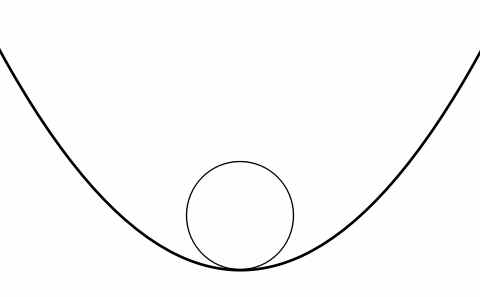
\includegraphics[width=\textwidth]{img/estabilidad1.png}
		\caption{Punto de equilibrio estable.}
		\label{fig:estabilidad1}
	\end{subfigure}
	\begin{subfigure}[b]{0.30\textwidth}
		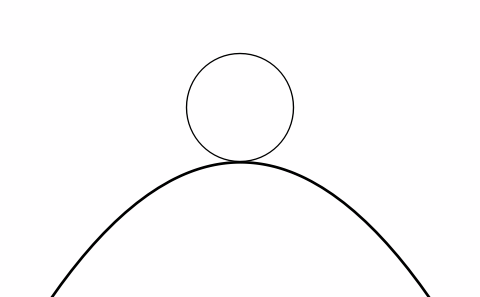
\includegraphics[width=\textwidth]{img/estabilidad2.png}
		\caption{Punto de equilibrio inestable}
		\label{fig:estabilidad2}
	\end{subfigure}
	\caption{Puntos de equilibrio.}
	\label{fig:estabilidad}
	
\end{figure}

Se dice que un sistema es BIBO (\textit{Bounded input bounded output}) estable si a entradas acotadas corresponden salidas acotadas.

Retomando el ejemplo de la figura \ref{fig:estabilidad}, si se aplica un desplazamiento hacia la derecha, en el caso \ref{fig:estabilidad1}, corresponde a una pequeña entrada a la que se le asigna una pequeña salida; por otro lado, si se le aplica una pequeña entrada al caso \ref{fig:estabilidad2}, la diferencia de la respuesta del sistema es mucho más grande \cite{dinamicos}.

\subsection{Invariante en el tiempo}

Se dice que un sistema es invariante en el tiempo si un corrimiento en el tiempo en la señal de entrada causa el mismo corrimiento en el tiempo de la señal de salida del sistema. Si $y(t)$ es la salida de un sistema cuando la entrada es $x(n)$, entonces $y(t - t_0)$ es la salida cuando se aplica la señal de entrada $x(t - t_0)$ \cite{dinamicos}.

\end{comment}

\begin{comment}
\section{Sistemas dinámicos}

Como ya se mencionó, un sistema dinámico es aquel en el cual existe un almacenamiento de energía, materia e información, es decir, es un sistema que posee memoria.



	De acuerdo con \cite{modelado_sis_det}, podemos definir a un sistema dinámico determinista de la siguiente manera.

\begin{definition}
	
	Un sistema dinámico determinista se define como una colección $D = <T, U, \Omega, Y, Q, \Delta, \varLambda>$ donde: 
	
	\begin{itemize}
		
		\item $T$ es la base del tiempo (el conjunto de valores posibles para la variable $t$).
		
		\item $U$ es el conjunto de valores posibles de la entrada.
		
		\item $\Omega$ es el conjunto de segmentos admisibles de entrada (sus elementos son funciones $\omega : [t_1, t_2] \subset T \to U$).
		
		\item $Y$ es el conjunto de valores de salida.
		
		\item $Q$ es el conjunto de valores posibles de los estados.
		
		\item $\Delta: Q \times \Omega \to Q$ es la función de transición de estados.
		
		\item $\varLambda: Q \to Y$ es la función de salida.
		
	\end{itemize}
	
\end{definition}

La función de transición $\Delta$ se caracteriza por:

\begin{itemize}
	
	\item Dado un segmento de entrada admisible $\omega: [t_1, t_2] \subset T \to U$ y sabiendo que el estado en $t_1$ es $q(t_1) \in Q$, entonces $q(t_2) = \Delta(q(t_1),\omega)$. Es decir, $\Delta$ transforma el estado inicial y la entrada en el estado final. 
	
	\item Dados dos segmentos de entrada admisibles consecutivos $\omega_1: [t_1, t_2] \to U$ y $\omega_2:[t_3, t_4] \to U$, y asumiendo que la concatenación $\omega_1 \circ \omega_2 \in \Omega$, debe cumplirse que $\Delta(q, \omega_1 \circ \omega_2) = \Delta(\Delta(q, \omega_1), \omega_2)$. Esta propiedad garantiza que la evolución del sistema sea compatible con el procesamiento secuencial de entradas.
	
\end{itemize}

\end{comment}

\section{Teoría del caos}

De acuerdo con \cite{Simon2025_caos}, el caos trata con sistemas cuyo comportamiento es impredecible a largo plazo. Suele ser asociado a sistemas aleatorios o que no tienen un orden, pero en teoría del caos se refiere a todos aquellos sistemas deterministas cuya predicción en instantes de tiempo futuro se vuelve difícil de calcular. 

Las condiciones iniciales suelen contener errores que incrementarán exponencialmente con el tiempo, lo que se conoce como sensibilidad a las condiciones iniciales, haciendo imposible la predicción a largo plazo. Estos se conocen como sistemas caóticos.

\begin{definition}
	Sea $X$ un espacio métrico y sea $\phi: X \to X$ una aplicación continua. Se dice que un sistema es caótico si cumple las siguientes condiciones:
	
	\begin{itemize}
		\item La aplicación $\phi: X \to X$ es topológicamente transitiva. 
		\item El conjunto de puntos de $\phi$ es denso en el atractor. 
		\item La aplicación $\phi: X \to X$ tiene dependencias sensitivas a las condiciones iniciales. 
	\end{itemize}	
	
\end{definition}

El hecho de que la aplicación sea topológicamente transitiva implica que el atractor caótico es irreducible, es decir, si iteramos la función $\phi$ un número determinado de veces (evolucionar el sistema durante un periodo de tiempo suficiente), se puede acceder a cualquier punto del atractor desde cualquier otro.

Si el conjunto de puntos es denso en el atractor, entonces cualquier punto en el espacio está arbitrariamente cerca de una órbita periódica. 

Finalmente, la sensibilidad a las condiciones iniciales refleja el hecho de que en un sistema caótico, dos trayectorias que inician relativamente cerca acabarán comportándose de una forma diferente a largo plazo. 

\begin{comment}
	\subsection{Exponentes de Lyapunov}

Para evaluar la sensibilidad de las condiciones se utilizan los exponentes de Lyapunov. Los cuales cuantifican la estabilidad o inestabilidad de las trayectorias en el espacio de fases al sufrir una perturbación ligera. Supongamos que tenemos dos trayectorias próximas separadas por una distancia $\delta \epsilon_0$; entonces la distancia entre ellas diverge de la forma:

\begin{equation}
	\delta_\epsilon(t) \sim \delta \epsilon_0 e^{\lambda t}
\end{equation}

Donde $\lambda$ es el exponente de Lyapunov. Es decir, mide la tasa de separación entre dos trayectorias cercanas en el espacio de fases. En un espacio de fases $n$-dimensional, existen $n$ exponentes de Lyapunov, lo que se conoce como espectro de Lyapunov. 
\end{comment}

\subsection{Atractores}

En un espacio disipado, la región del espacio de fases que atrae a las trayectorias vecinas se conoce como atractor. Es un subconjunto en el espacio de fases, es decir, un conjunto de estados a los que tiende a evolucionar el sistema en función de las condiciones iniciales.

\begin{definition}
	Sea $X$ el espacio de fases de un sistema dinámico disipado y sea $\phi_t: X \to X$ la transformación que describe el movimiento. Se dice que $A \subset X$ es un atractor si verifica las siguientes condiciones:
	
	\begin{itemize}
		
		\item $\exists U$ entorno de $A$, llamado cuenca de atracción de $A$, tal que $\forall V$ abierto con $A \subset V$, existe un $T_0$ tal que $\phi_t(U) \subset V, \forall t > T_0$.
		
		\item $\phi_t(A) = A, \forall t > 0$
		
		\item $\nexists S \subset A$ subconjunto propio no vacío que satisfaga las dos propiedades anteriores.
		
	\end{itemize} 
	
\end{definition} 

Es decir, un punto que se encuentra en el atractor no puede salir de ahí y existe una órbita alrededor de este en donde, para cualquier tiempo, la trayectoria permanece en la órbita.

\subsubsection{Tipos de atractores}

A continuación, se describen los cuatro tipos de atractores que se encuentran en la figura \ref{fig:atractores}.

\begin{enumerate}
	
	\item Atractores de punto fijo:  Un atractor es de punto fijo si existe un punto fijo tal que todas las trayectorias cercanas convergen a el cuando $t \to \infty$.

	La figura \ref{fig:punto_fijo} muestra el comportamiento de  un péndulo con resistencia al viento que responde a la ecuación:
	\begin{equation*}
		\theta'' + \gamma \theta' + \beta \theta' |\theta'| + \frac{g}{L} \sin(\theta) = 0
	\end{equation*}
	La energía se disipa por la fricción $\gamma$ y por la resistencia del aire $\beta$, obligando al sistema a perder velocidad hasta detenerse en el origen.

	\item Atractores de ciclo límite: Las trayectorias vecinas se acercan o se alejan del ciclo límite en forma de espiral. 
	
	En la figura \ref{fig:ciclo_limite} se muestra el oscilador de Van der Pol, cuya dinámica esta definida por:
	\begin{equation*}
		x'' - \mu (1 - x^2) x' + x = 0
	\end{equation*}
	El sistema aumenta la energía cuando la amplitud es pequeña y la disipa si es grande, por lo que todas las trayectorias convergen a una órbita periódica estable. 
	
	\item Atractores cuasiperiódicos: Cuando dos ciclos límites con diferentes trayectorias se superponen, estas se enroscan en las direcciones longitudinales y latitudinales, creando una figura toroidal.
	
	La Figura \ref{fig:cuasi_periodico} ilustra un oscilador lineal forzado con una frecuencia externa basada en la razón áurea $\phi$:
	\begin{equation*}
		x'' + x = A \cos(\phi t)
	\end{equation*}
	Debido a que $\phi$ es irracional respecto a la frecuencia del oscilador, el movimiento resultante es una superposición de trayectorias que nunca se repiten exactamente.
	
	\item Atractores extraños: Se dice que un atractor es extraño si tiene dimensión fractal (patrón de autosimilitud a diferentes escalas). Además, un atractor extraño es caótico si las trayectorias del sistema son atraídas hacia él, pero dentro del atractor son inestables. Esto significa que son sensibles a las condiciones iniciales.
	
	La Figura \ref{fig:caotico} muestra el atractor de Rössler, definido por el siguiente sistema de ecuaciones:
	\begin{equation*}
		\begin{cases}
			x' = -y - z \\
			y' = x + ay \\
			z' = b + z(x - c)
		\end{cases}
	\end{equation*}
	Las trayectorias se atraen hacia una estructura geométrica compleja donde se estiran y se pliegan continuamente, lo que genera un comportamiento impredecible a largo plazo a pesar de ser un sistema determinista.
\end{enumerate}

\begin{figure}[!htbp]
	\centering
	\begin{subfigure}[b]{0.40\textwidth}
		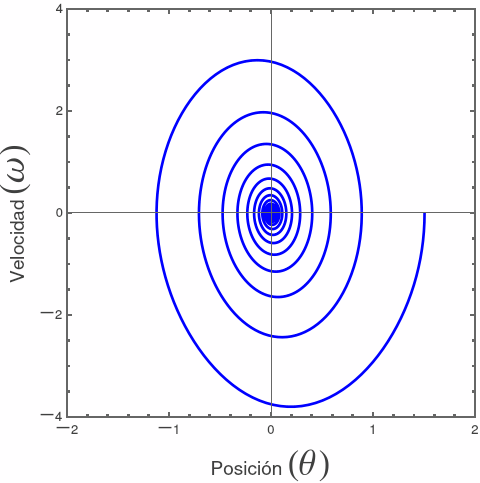
\includegraphics[width=\textwidth]{img/punto_fijo.png}
		\caption{Punto fijo: Convergencia al reposo en un péndulo amortiguado.}
		\label{fig:punto_fijo}
	\end{subfigure}
	\begin{subfigure}[b]{0.40\textwidth}
		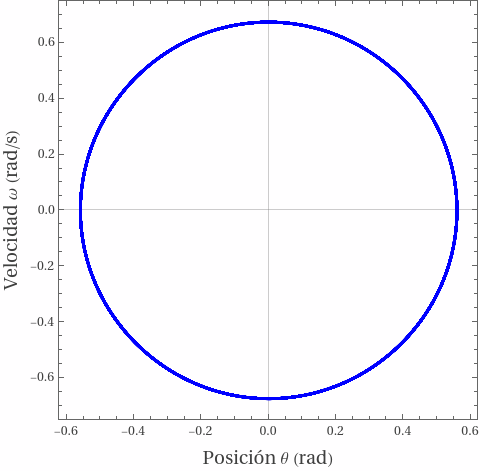
\includegraphics[width=\textwidth]{img/ciclo_limite.png}
		\caption{Ciclo límite: Oscilador de Van der Pol.}
		\label{fig:ciclo_limite}
	\end{subfigure}
	\begin{subfigure}[b]{0.40\textwidth}
		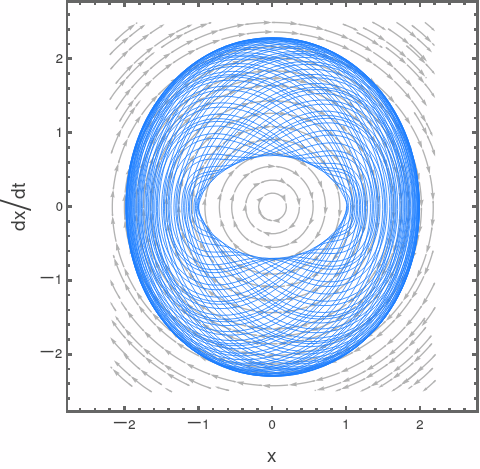
\includegraphics[width=\textwidth]{img/cuasiperiodico.png}
		\caption{Cuasiperiódico: Trayectoria densa generada por frecuencias inconmensurables.}
		\label{fig:cuasi_periodico}
	\end{subfigure}
	\begin{subfigure}[b]{0.40\textwidth}
		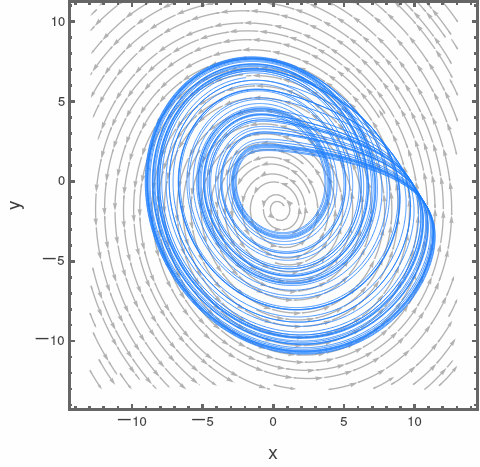
\includegraphics[width=\textwidth]{img/caotico.png}
		\caption{Extraño: Atractor de Rössler que exhibe una estructura fractal y caos.}
		\label{fig:caotico}
	\end{subfigure}
	\caption{Representación de los cuatro tipos principales de atractores en el espacio de fases.}
	\label{fig:atractores}
\end{figure}

\section{Sistemas complejos}

Los sistemas complejos son sistemas dinámicos con muchas componentes que interactúan entre sí mediante el intercambio de materia, energía o información y que, eventualmente, sufren la acción de agentes externos \cite{Torres2025_complejo}. Las colonias de hormigas, el mercado bursátil, el clima, el sistema nervioso, las células y los organismos vivos son algunos ejemplos de sistemas complejos. Estos se caracterizan por tener un conjunto de elementos que interactúan entre sí con el fin de alcanzar un objetivo \cite{Zelinka2014_cs, Zelinka2018_cs}. 

Los sistemas complejos tienen dos implicaciones fundamentales: (1) Existe una influencia mutua entre sus elementos, donde el cambio afecta inevitablemente al resto de elementos, y (2) persiguen un objetivo \cite{Zelinka2018_cs}. Además, de acuerdo con \cite{sole1996_cs_caos}, los sistemas complejos están estrechamente relacionados con la teoría del caos, pues la interacción de múltiples elementos locales puede llevar al sistema completo a lo que llama ``borde del caos'', una región donde el sistema es lo suficientemente estable para mantener su estructura, pero se mantiene flexible para generar nuevos patrones.

\begin{definition}
	Un sistema complejo es una entidad compuesta de partes interconectadas, de tal forma que el comportamiento colectivo es más que la suma de sus componentes individuales.
\end{definition}

Para entender el comportamiento de un sistema es necesario conocer los elementos y sus interacciones. Es decir, se requiere conocer los estados, valores instantáneos de todos los elementos; y sus transiciones, es decir, los cambios dinámicos en los estados.

Los sistemas complejos se caracterizan principalmente por:

\begin{itemize}
	
	\item \textbf{No linealidad}: No cumple el principio de superposición, es decir, el resultado no puede expresarse como la suma de las respuestas individuales a cada estímulo por separado. Resulta difícil predecir su evolución dinámica futura \cite{Zelinka2018_cs, Moriello2003_cs}.

	\item \textbf{Retroalimentación}: Las salidas pasadas influyen en las siguientes salidas. Este comportamiento hace alusión a la memoria del sistema \cite{Moriello2003_cs}. 
	
	\item \textbf{Orden espontáneo}: Existe un orden emergente resultado de las interacciones locales no coordinadas, el cual no puede ser descrito mediante sus interacciones locales \cite{Moriello2003_cs}.
	
	\textbf{Aparición (\textit{emergence})}: Entidades, patrones, comportamientos y propiedades emergen de la interacción de entidades más pequeñas, las cuales no exhiben estos atributos \cite{Moriello2003_cs}.

	\textbf{Elementos múltiples}: Compuesto de múltiples elementos relativamente idénticos con interacciones locales \cite{Zelinka2018_cs}. 
\end{itemize}

\section{Modelado de sistemas complejos}

Resulta evidente que predecir el comportamiento de estos sistemas es una tarea complicada. Una aproximación es el uso de modelos científicos y matemáticos, los cuales se construyen para desarrollar procesos de inferencia sobre aspectos observados en la vida real. El modelo de inferencia se realiza para entender el sistema real observado.

El proceso, de manera simplificada, se compone de tres fases, como se observa en la figura \ref{fig:cs_cientifico}:

\begin{itemize}
	
	\item Se abstrae el sistema real a un modelo, el cual puede trascender a otros sistemas reales.
	
	\item El modelo realiza un proceso de inferencia que busca averiguar las implicaciones derivadas de las premisas.
	
	\item Los resultados se utilizan para analizar, interpretar y aplicar a un sistema real. Esta aplicación no requiere ser práctica; es una relación entre las inferencias obtenidas con el modelo y el sistema real.
	
\end{itemize}

\begin{figure}[H]
	
	\centering
	
	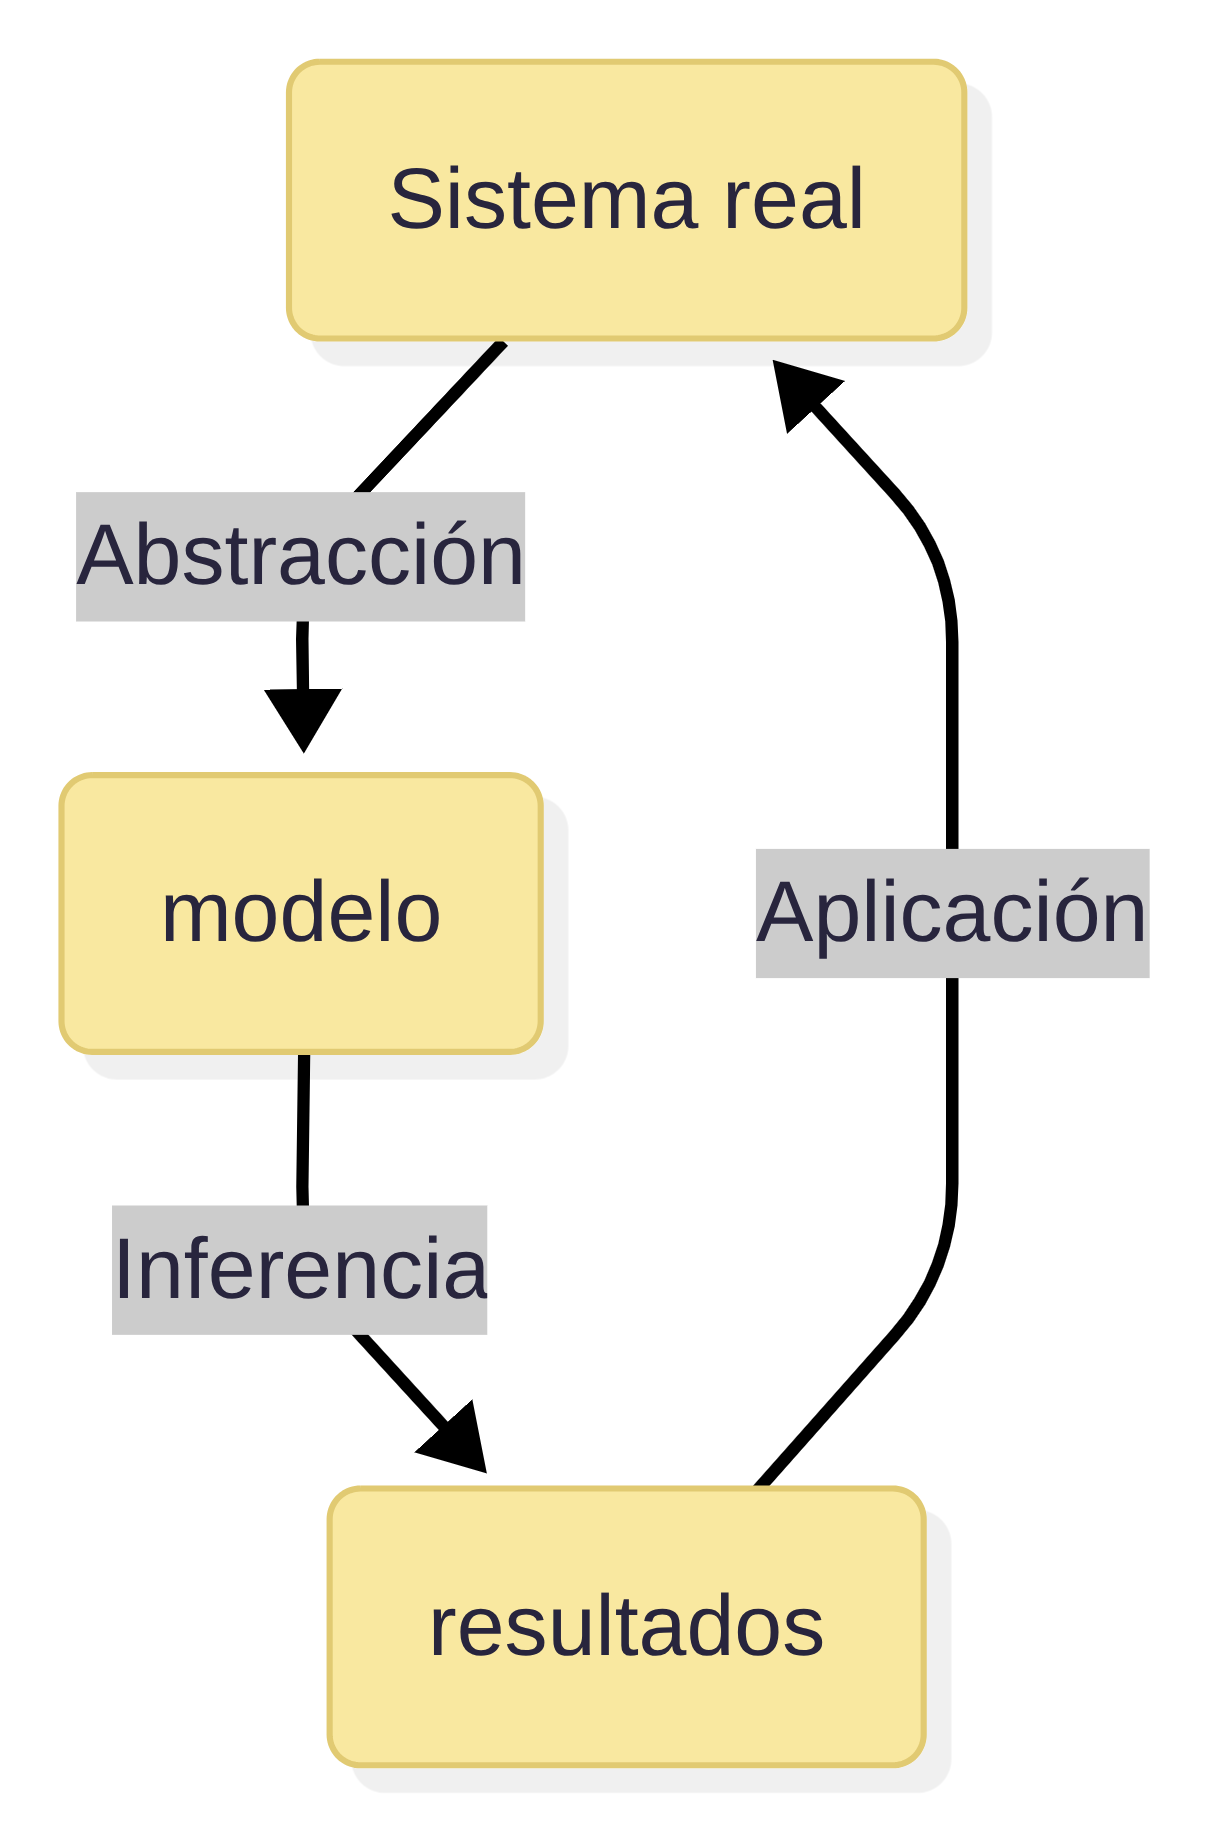
\includegraphics[width=0.3\linewidth]{img/cs_cientifico.png}
	
	\caption{Representación gráfica del modelado científico. Este proceso busca relacionar eventos del mundo real utilizando un modelo que realiza una inferencia.}
	
	\label{fig:cs_cientifico}
	
\end{figure}

%Definir que es simular

Sin embargo, estos modelos suelen carecer de las herramientas necesarias que les permiten deducir las implicaciones lógicas necesarias. Es aquí donde la computación permite agilizar este proceso realizando simulaciones.

Las computadoras permiten explorar y analizar modelos formales para resolver modelos matemáticos. Además, dado que un modelo computacional puede ser definido mediante un modelo matemático, el rol de la computación es simplificar este proceso. Dicho esto, \cite{gamco2024_simulacion} define a la simulación de la siguiente manera:

\begin{definition}
	Simulación es un proceso computacional que permite imitar el comportamiento de un sistema mediante la utilización de un modelo matemático.
\end{definition}

Los resultados de la simulación provienen del uso de reglas algorítmicas. Por eso, es necesario ampliar el proceso de abstracción y crear un modelo formal que será utilizado por la computadora, como se muestra en la figura \ref{fig:cs_computacional}.

\begin{figure}[H]
	
	\centering
	
	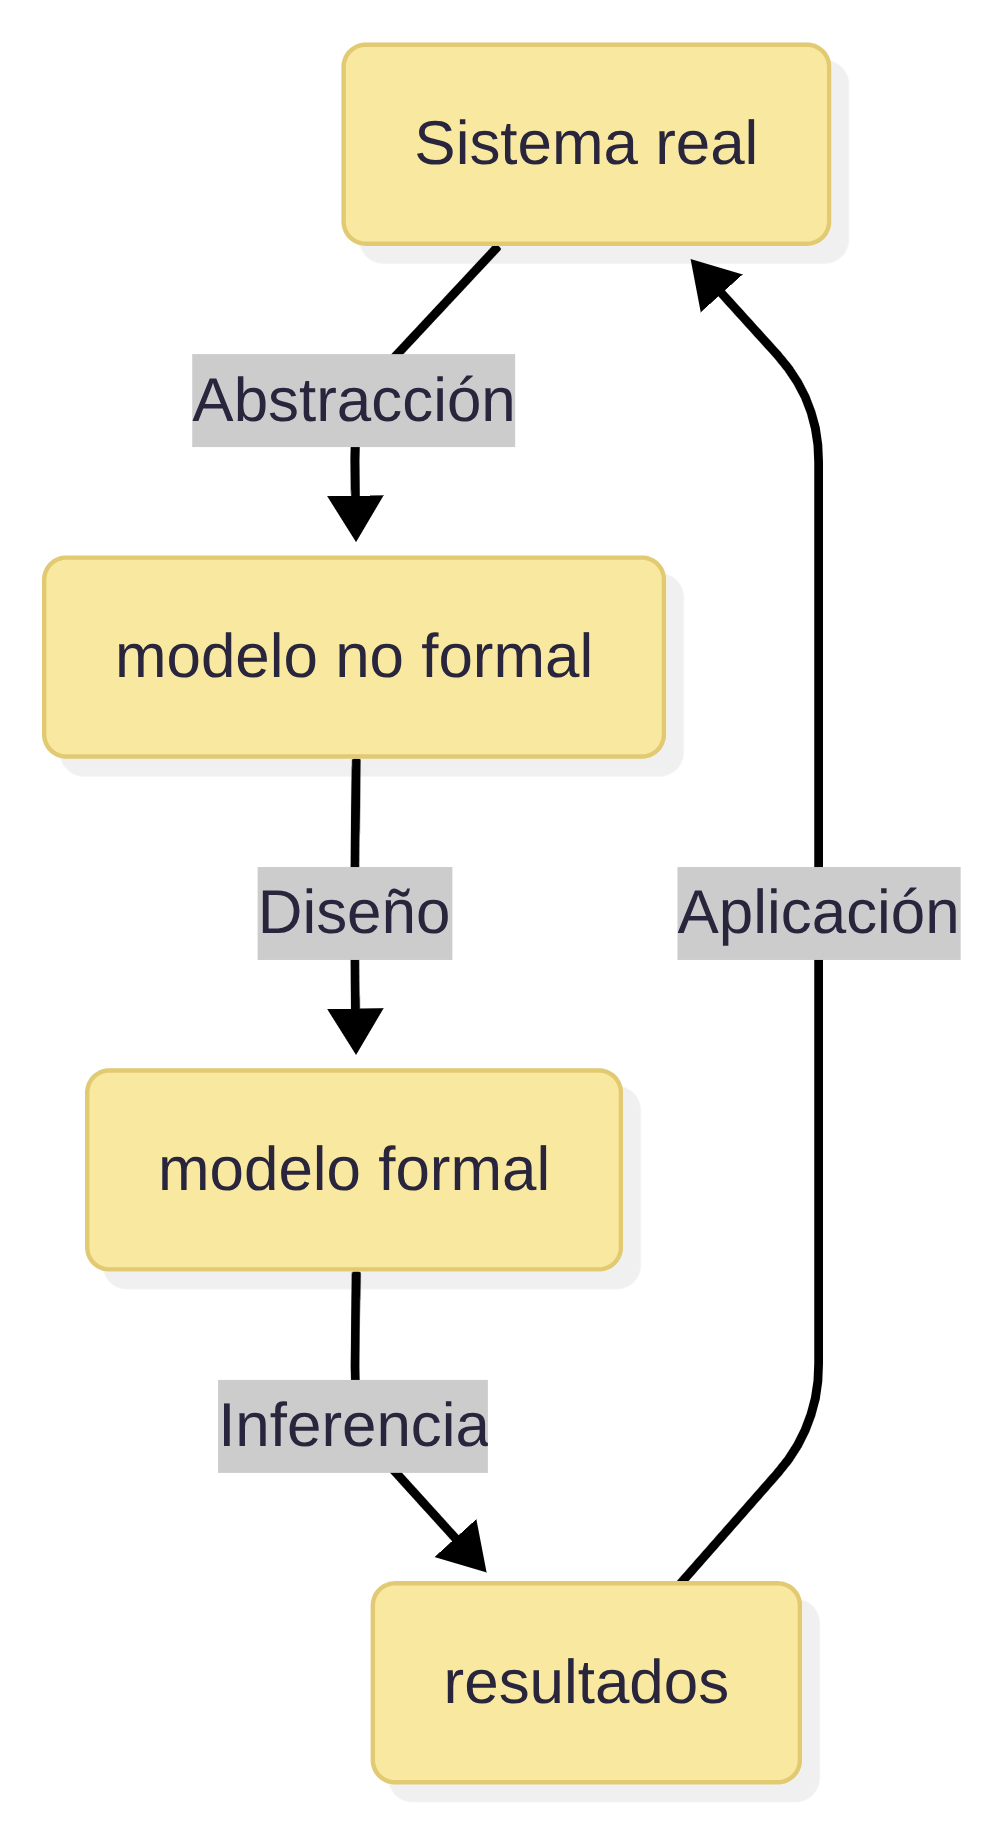
\includegraphics[width=0.3\linewidth]{img/cs_computacional.png}
	
	\caption{Representación gráfica del modelado computacional. Relaciona eventos del mundo real utilizando un modelo computacional que ayuda a agilizar el proceso de inferencia.}
	
	\label{fig:cs_computacional}
	
\end{figure}

Se requiere de un experto en el sistema real que pueda abstraer el problema y un modelador que formalice dicha abstracción para ejecutarla en una computadora que infiera los resultados, mismos que utilizará nuevamente el experto en el sistema real para entablar la relación con el sistema real \cite{Izquierdo2008_modelado}.

Para estudiar sistemas complejos hay varias herramientas de simulación. Una de ellas son los autómatas celulares \cite{Torres2025_complejo, sole1996_cs_caos, Hoekstra2010_cs_ca}, los cuales siguen la caracterización de los sistemas complejos: elementos idénticos con interacciones locales que pueden generar orden espontáneo, comportamientos emergentes e incluso retroalimentados. 
\clearpage
	\chapter{Marco teórico: Autómatas celulares}
\label{chapter:automatas_celulares}

La investigación de los sistemas complejos es un reto actual de la ciencia moderna. Estos sistemas, caracterizados por la interacción entre múltiples componentes locales, son capaces de generar comportamientos emergentes y, a veces, caóticos. Para entender esta complejidad necesitamos herramientas que puedan capturar la esencia de la autoorganización, y aquí los autómatas celulares surgen como un modelo computacional clave para simular fenómenos tanto naturales como artificiales.

En este capítulo se definen los fundamentos matemáticos y estructurales de un autómata celular. Este se entiende como un sistema dinámico discreto, que combina un conjunto de celdas interconectadas y que pueden producir patrones complejos a partir de reglas locales. Se mencionarán sus elementos esenciales, tales como:

\begin{itemize}
	
	\item El vecindario: El subconjunto de celdas que afecta el cambio de una unidad.
	
	\item El estado de conjunto: Los valores finitos que puede tomar cada celda.
	
	\item Las condiciones de frontera son: El comportamiento del sistema en sus límites en el espacio.
	
	\item Las funciones de transición son: El algoritmo que rige la evolución del sistema.
	
\end{itemize}

Se revisan, asimismo, ejemplos que han sido de una importancia capital para el desarrollo de esta disciplina, tales como el Juego de la Vida de John Conway y los autómatas celulares elementales de Stephen Wolfram.

Finalmente, el capítulo amplía la definición clásica hacia terrenos más avanzados. Se presentan autómatas celulares que operan en espacios no euclidianos y se examinan extensiones recientes que incluyen estados continuos, reglas de probabilidad o actualizaciones asíncronas. Estas variaciones hacen que los AC continúen siendo, décadas después de ser concebidos por Von Neumann, una herramienta de vanguardia en campos tan diversos como la biología teórica, la criptografía y la física de partículas.

\section{Autómata celular}

Los autómatas celulares, concebidos por John von Neumann en 1948 \cite{damerow2010_neumann}, son una colección de células donde cada una de ellas puede adquirir un estado y se agrupan en una red. Además, estas células evolucionan en intervalos y cada una de ellas actualiza su estado en función del estado de sus células vecinas \cite{weisstein2002_ca, wolfram1982_ca, fsancho2016_ca}. 

Siguiendo de manera general a \cite{bhattacharjee2019_ca, sayama2024_ca, Ilachinski2001_ca}, y considerando una red regular de células, un conjunto finito de estados y evoluciones en pasos discretos de tiempo, se define a un autómata celular como:

\begin{definition}
	Un autómata celular es una 4-tupla ($\mathcal{L}, \mathcal{S}, \mathcal{N}, \mathcal{R}$) donde:
	\begin{itemize}
		\item $\mathcal{L} \subseteq \mathbb{Z}^D$ es el espacio celular $D$-dimensional. El conjunto de células vive en el espacio $\mathcal{L}$ y cada célula $\vec{i}$ se define como un vector $D$-dimensional que representa su posición en el espacio.
		
		\item $\mathcal{S}$ es un conjunto de $k$ estados. Cada célula $\vec{i}$ solo puede adquirir un valor de un conjunto finito de diferentes estados:	
		\[
		\sigma_{\vec{i}}(t) \in \mathcal{S} \equiv \{ s_0, s_1,s_2, \dots, s_{k - 1} \},\; \forall \vec{i} \in \mathcal{L}
		\]
		Donde $\vec{i} \in \mathcal{L}$ es una célula en el espacio celular, $\sigma_{\vec{i}} (t)$ es el estado de la i-ésima célula en el tiempo $t$ y $\mathcal{S}$ es un anillo conmutativo finito, como un intervalo de números enteros, que generalmente se define por los enteros módulo $k$ ($\mathbb{Z}_k$).
			
		\item $\mathcal{N} = (\vec{v}_1, \vec{v}_2, \dots, \vec{v}_m )$ es el conjunto de los $m$ vectores de desplazamiento que definen la vecindad de una célula en $\mathcal{L}$. Así, los vecinos de las células ubicadas en $\vec{i} \in \mathcal{L}$ se encuentran en las posiciones $\vec{i} + \vec{v}, \forall \vec{v} \in \mathcal{N}$ 
		
		\item $\mathcal{R} : \mathcal{S}^m \to \mathcal{S}$ es la regla local del autómata:
		\[
		\sigma_{\vec{i}}(t + 1) = \mathcal{R} ( \{ \sigma_{\vec{i} + \vec{v}_j}\}_{j = 1}^m  )
		\]
		donde $\mathcal{R}$ es la función de transición local que asigna el nuevo estado de una célula a partir de los estados de sus $m$ vecinos.		
	\end{itemize}
	
\end{definition}

\section{Vecindad}

Como ya se mencionó, la vecindad es el conjunto de vectores de desplazamiento, por lo que está estrechamente relacionado con la dimensionalidad del autómata celular. Por ejemplo, John von Neumann propuso una vecindad para $\mathbb{Z}^2$ de cinco células que actualmente se conoce como vecindad de von Neumann. Esta vecindad considera a la célula y a sus cuatro vecinas ortogonales más cercanas \cite{neumann1966_ca}, dicho de otro modo:
\[
	\mathcal{N} = ((0, -1), (-1, 0), (0, 0), (1, 0), (0, 1))
\]
La cual se puede representar como en la figura \ref{fig:N_neumann}. 

Por otro lado, Moore añade los cuatro vecinos diagonales más cercanos a la vecindad de von Neumann, dando una vecindad de nueve elementos \cite{Kwon2015_moore}. Esta vecindad, representada por la figura \ref{fig:N_moore}, fue utilizada por John Conway en el ``Juego de la Vida'' \cite{lifewiki_life}.

Otro ejemplo se encuentra en la figura \ref{fig:N_wolfram}, la cual representa una vecindad de radio uno en un espacio unidimensional, es decir, todas aquellas células a una distancia menor o igual a uno, incluyéndose a su misma. Fue utilizada por Stephen Wolfram para definir los autómatas celulares elementales \cite{Wolfram2002_nks}.

\begin{figure}[!htbp]
	\centering
	\begin{subfigure}[b]{0.30\textwidth}
		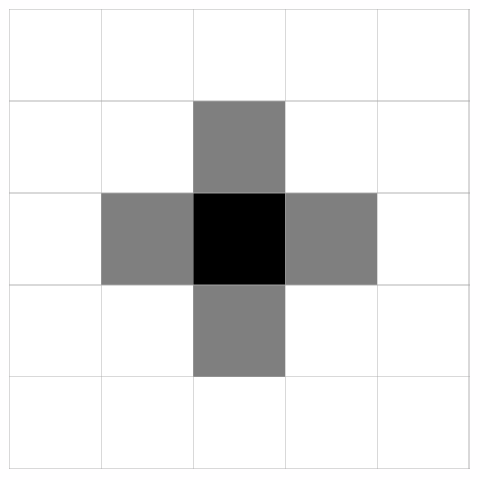
\includegraphics[width=\textwidth]{img/nNeumann.png}
		\caption{Vecindad de von Neumann}
		\label{fig:N_neumann}
	\end{subfigure}
	\begin{subfigure}[b]{0.30\textwidth}
		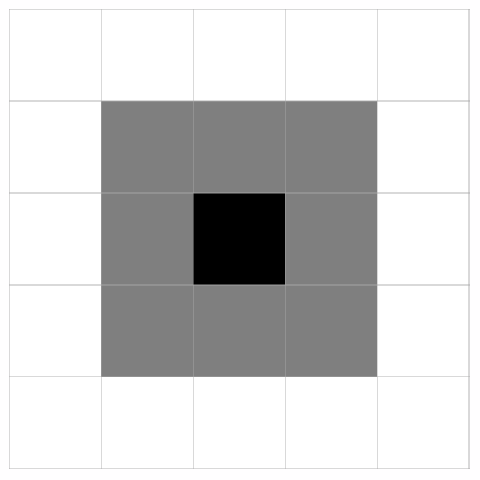
\includegraphics[width=\textwidth]{img/nMoore.png}
		\caption{Vecindad de Moore}
		\label{fig:N_moore}
	\end{subfigure}
	\begin{subfigure}[b]{0.40\textwidth}
		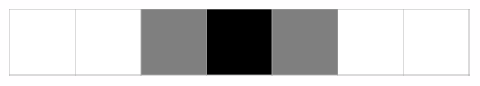
\includegraphics[width=\textwidth]{img/nWolfram.png}
		\caption{Vecindad de radio uno en $\mathbb{Z}^1$}
		\label{fig:N_wolfram}
	\end{subfigure}
	\caption{Las vecindades \ref{fig:N_neumann} y \ref{fig:N_moore} son para CA bidimensionales; la \ref{fig:N_wolfram} es para CA unidimensionales. La célula negra representa la célula actual y, junto con las grises, conforma su vecindad.}
	
	\label{fig:vecindades_regulares}
	
\end{figure}

Las vecindades no solo son cuadradas; también pueden tener otras formas, como hexágonos o triángulos, que se muestran en las figuras \ref{fig:N_hexagonal} y \ref{fig:N_triangular}.  Además, existen vecindades con comportamiento dinámico, como la de Margolus mostrada en la figura \ref{fig:N_margolus}, cuya configuración alterna entre dos disposiciones en cada paso evolutivo \cite{tyler2018_margolus}.

\begin{figure}[!htbp]
	\centering
	\begin{subfigure}[b]{0.30\textwidth}
		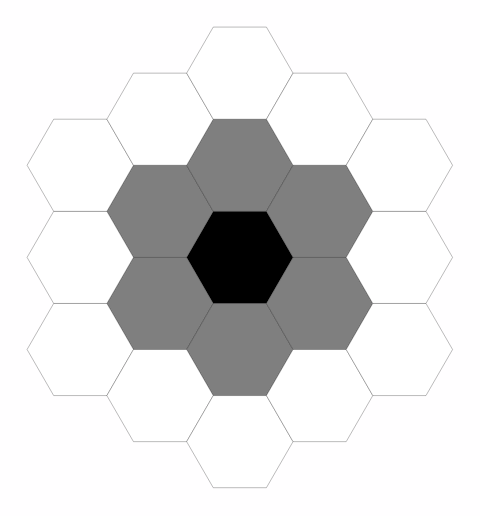
\includegraphics[width=\textwidth]{img/nHexagon.png}
		\caption{Vecindad hexagonal}
		\label{fig:N_hexagonal}
	\end{subfigure}
	\begin{subfigure}[b]{0.30\textwidth}
		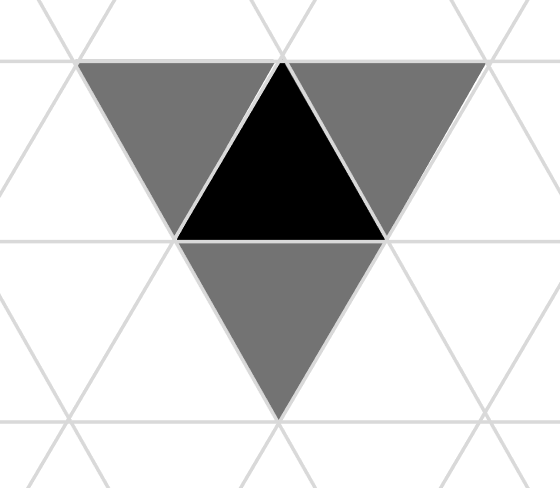
\includegraphics[width=\textwidth]{img/nTriangular.png}
		\caption{Vecindad triangular}
		\label{fig:N_triangular}
	\end{subfigure}
	\begin{subfigure}[b]{0.30\textwidth}
			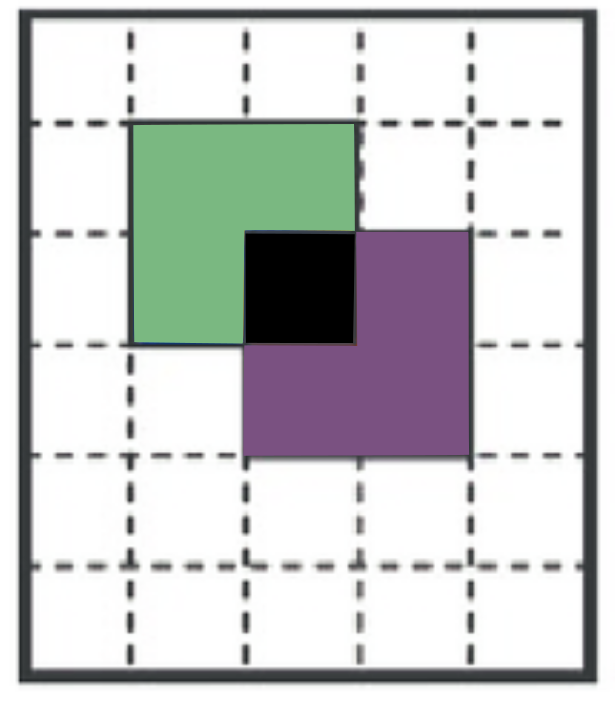
\includegraphics[width=\textwidth]{img/nMargolus.png}
		\caption{Vecindad de Margolus}
		\label{fig:N_margolus}
	\end{subfigure}
	
	\caption{En \ref{fig:N_hexagonal} y \ref{fig:N_triangular}, la célula negra es la actual y las grises su vecindad.  En \ref{fig:N_margolus}, la célula negra es la actual, mientras que las células verdes y moradas representan las vecindades activas en tiempos pares e impares.}
	
	\label{fig:vecindades_irregulares}
	
\end{figure}

Finalmente, los vecinos no tienen que ser estrictamente adyacentes entre sí ni ser simétricos. Existen vecindades, como en la figura \ref{fig:N_noadyacente}, donde algunas células no son contiguas a la central.

\begin{figure}[!htbp]
	\centering
	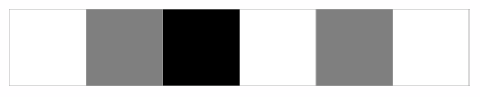
\includegraphics[width=0.5\textwidth]{img/nNoAdyacente.png}
	\caption{Vecindad en $\mathbb{Z}^1$ con vecinos de adyacentes.}
	\label{fig:N_noadyacente}
\end{figure}

\section{Estados}

Cada célula adquiere un único estado $s$ en cada paso de tiempo, donde $s$ pertenece a un conjunto de estados $s \in \mathcal{S}$. Por ejemplo, el autómata celular de John von Neumann contempla 29 estados, aunque algunos autores han propuesto variantes reducidas a cuatro estados, conservando su capacidad de autoreproducirse \cite{bhattacharjee2019_ca}. 

Por otro lado, el juego de la vida se compone de dos estados que denominó ``vivas'' y ``muertas'' \cite{lifewiki_life}.  De igual forma, Stephen Wolfram utiliza dos estados en los autómatas celulares elementales \cite{Wolfram2002_nks}.

Idealmente, el espacio celular $\mathcal{L}$ es infinito, lo que permitiría infinitas combinaciones de estados. Sin embargo, esto es inviable computacionalmente. Para esto, se requiere establecer una restricción de finitud, como lo marca \cite{bhattacharjee2019_ca}.
 
 Supóngase un espacio discreto unidimensional infinito. Idealmente, conocemos el estado de las infinitas células, pero computacionalmente no podemos almacenar ni procesar toda esa información. Por lo que se restringe a los valores que únicamente nos interesan. 
 
 A todas aquellas células que son de interés se les define con un estado activo, el cual puede ser cualquier $s \in \mathcal{S}$, por otro lado, las que no son de interés se les define con un estado inactivo $\sigma_q$:
 
\begin{definition}
	Sea $\mathcal{R}$ la regla local de un autómata celular. Un estado $\sigma_q \in \mathcal{S}$ es inactivo si $\mathcal{R}(\sigma_q, \sigma_q, \dots, \sigma_q) = \sigma_q$.
	\label{def:estado_inactivo}
\end{definition}

Es decir, si una célula y todos sus vecinos están en estado inactivo, la célula permanece inactiva tras aplicar $\mathcal{R}$. Cabe notar que todos los vecinos deben estar en dicho estado, por lo que, si alguno cambia a cualquier estado $s$, entonces se  activa. Este evento ocurre cuando el espacio en donde evoluciona el autómata celular incrementa. 

Para trabajar computacionalmente, \cite{bhattacharjee2019_ca} define las configuraciones finitas de la siguiente manera:

\begin{definition}	
	Sea $\sigma_q \in \mathcal{S}$ un estado inactivo, $\sigma_p \neq \sigma_q \in \mathcal{S}$ un estado no inactivo y sea $\mathcal{L}$ un espacio celular infinito. Se considera que un autómata celular tiene configuración finita si solo un número finito de celdas están en estados activos $\sigma_p$.
\end{definition}

Si la configuración inicial es finita, la propiedad de finitud se preserva en cada paso de tiempo, como se observa en la tabla \ref{tab:CA_finito}. Imaginemos un autómata celular en $\mathbb{Z}^1$ con una vecindad de radio 1 y una sola célula activa en la posición $n$ con estado $\sigma_p$, mientras que el resto de infinitas células tienen estado inactivo $\sigma_q$. 

En el tiempo $t + 1$ las células en $n - 1$ y en $n + 1$ tienen un vecino que no es inactivo, por lo que pasan a ser activas por la definición \ref{def:estado_inactivo}. Dado que este incremento está acotado por el tamaño de la vecindad, la configuración resultante sigue siendo finita. Por inducción, este proceso se repite para cualquier tiempo $t + m$; por lo tanto, mientras el tiempo de la evolución no tienda a infinito ($t \not\to \infty $) el autómata celular mantendrá una configuración finita, garantizando su viabilidad computacional.

\begin{table}
	\centering
	\begin{tabular}{c | c c c c c c c c c c c} 
		$t$ & \multicolumn{11}{c}{ $\vec{\sigma}(t)$  } \\ \hline \hline
		0 & && & \dots & $q$ & $p$ & $q$ & \dots & && \\ \hline
		1 & & & \dots & $q$ & $p$ & $p$&  $p$ & $q$ & \dots & & \\ \hline
		2  & & \dots & $q$  & $p$ & $p$ & $p$&  $p$ &  $p$& $q$ & \dots &  \\ \hline
		3 & \dots & $q$  & $p$ & $p$ & $p$&  $p$&$p$ &$p$& $p$ & $q$ & \dots \\
	\end{tabular}
	\caption{Evolución temporal de un autómata celular unidimensional con una configuración inicial finita. Donde $p$ representa estados activos y $q$ estados inactivos. Los conjuntos $\vec{\sigma} (t)$ y $\vec{\sigma} (t + n)$ son finitos.}
	\label{tab:CA_finito}
\end{table}

Sea $\mathcal{C} =  \mathcal{S}^\mathcal{L}$ el conjunto de todas las configuraciones. Definimos $\mathcal{C}_F \subset \mathcal{C}$ como el subconjunto de todas las configuraciones finitas. Esta restricción es necesaria para hacer computacionalmente viable la simulación de la evolución.

\begin{comment}
	Finalmente, resulta necesario definir un estado estable, el cual servirá más adelante para establecer una clasificación \cite{bhattacharjee2019_ca}. 

\begin{definition}
	
	Dado un autómata celular y un estado $s \in \mathcal{S}$, se dice que $s$ es un estado estable si $\mathcal{R}(s, s, \dots, s) = s$.
	
\end{definition}

Esto es, un estado estable $s$ que evoluciona siempre en sí mismo, por lo que $\sigma(t) = \sigma(t + 1)$. 
\end{comment}

\section{Condiciones de frontera}

Idealmente, los autómatas celulares pueden evolucionar en espacios infinitos; sin embargo, se pueden establecer límites o fronteras, las cuales restringen el espacio celular $\mathcal{L}$ \cite{bhattacharjee2019_ca, ponce2015_ca}.

\begin{definition}
	Un autómata celular es finito si el espacio celular $\mathcal{L} \subseteq \mathbb{Z}^D$ es finito; en caso contrario, se denomina infinito. 
\end{definition}

Un autómata celular finito siempre tiene fronteras en los límites de su espacio. A la forma en como se comporta la frontera se le conoce como condición de frontera, la cual suele ser abierta o periódica \cite{ponce2015_ca}.

\begin{itemize}
	\item \textbf{Condición de frontera abierta}: Se les asigna un estado fijo a todos aquellos vecinos faltantes en las células de la frontera. 
	\item \textbf{Condición de frontera periódica}: Los vecinos faltantes de las células en la frontera son otras células en la frontera. La figura \ref{fig:B_periodica} muestra cómo se conectan las células de la frontera en un espacio unidimensional.
\end{itemize}

\begin{figure}[!htbp]
	\centering
	\begin{subfigure}[b]{0.45\textwidth}
		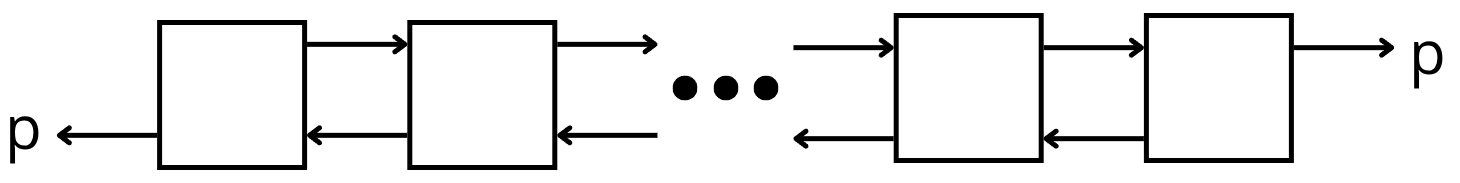
\includegraphics[width=\textwidth]{img/bAbierta.png}
		\caption{Condición de frontera abierta}
		\label{fig:B_abierta}
	\end{subfigure}
	\begin{subfigure}[b]{0.45\textwidth}
		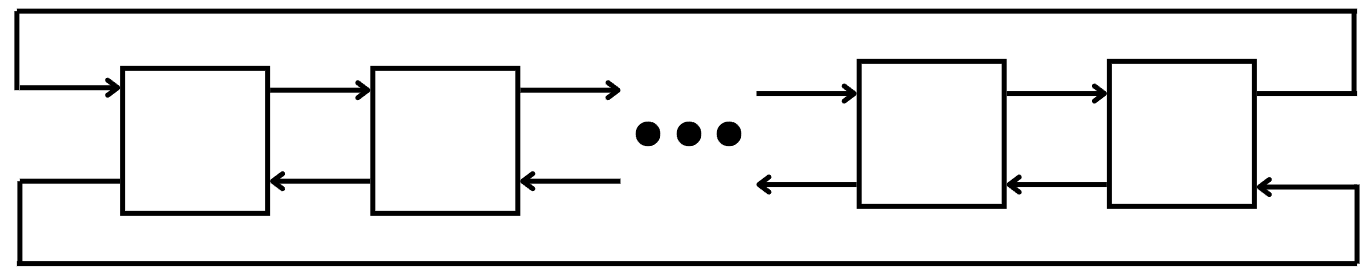
\includegraphics[width=\textwidth]{img/bPeriodica.png}
		\caption{Condición de frontera periódica}
		\label{fig:B_periodica}
	\end{subfigure}
	
	\caption{Condiciones de frontera con dos vecinos. La figura \ref{fig:B_abierta} asigna un estado no inactivo al vecino faltante. La figura \ref{fig:B_periodica} asigna como vecino el estado de la célula en la frontera opuesta, formando un anillo.}
	
	\label{fig:fronteras}
	
\end{figure}

Un autómata infinito que tiene una configuración periódica equivale a un autómata finito con frontera periódica \cite{bhattacharjee2019_ca}.

\begin{definition}
	Una configuración $\vec{\sigma} \in \mathcal{C}$ de un autómata celular $D$-dimensional se dice periódica si es invariante ante un conjunto de traslaciones linealmente independientes en $D$ direcciones. Es decir:
	\[
	\vec{\sigma} = T_i^{n_i} (\vec{\sigma}), \; \forall i \in \{ 1,2, \dots, D \}
	\]
	donde  $T_i^{n_i}$ denota un desplazamiento de $n_i$ posiciones en la dimensión $i$.
\end{definition}

Definimos entonces a $\mathcal{C}_P \subset \mathcal{C}$ como el conjunto de todas las configuraciones periódicas. Estas configuraciones preservan la condición de frontera periódica en cada traslación \cite{bhattacharjee2019_ca}. 

La frontera no solo puede ser abierta o periódica, existen diferentes comportamientos como la reflectiva y la reflexiva. La frontera reflectiva asigna a los vecinos faltantes el mismo estado de la célula en la frontera (figura \ref{fig:B_reflectiva}), por lo que son vecinas de si mismas. La frontera reflexiva, en cambio, genera una doble relación de vecindad en los extremos (figura \ref{fig:B_reflexiva}), \cite{bhattacharjee2019_ca, ponce2015_ca}.

\begin{figure}[!htbp]
	\centering
	\begin{subfigure}[b]{0.45\textwidth}
		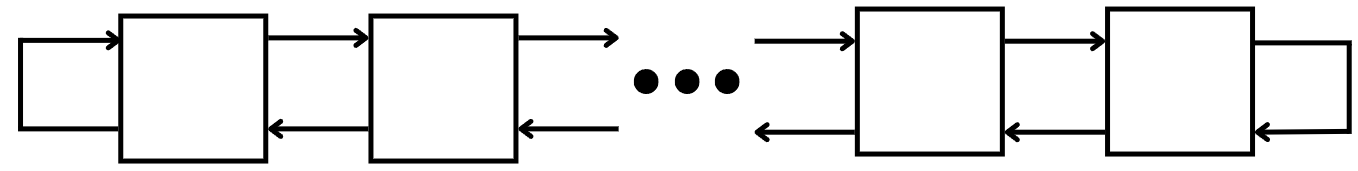
\includegraphics[width=\textwidth]{img/bReflectiva.png}
		\caption{Condición de frontera reflectiva}
		\label{fig:B_reflectiva}
	\end{subfigure}
	\begin{subfigure}[b]{0.45\textwidth}
		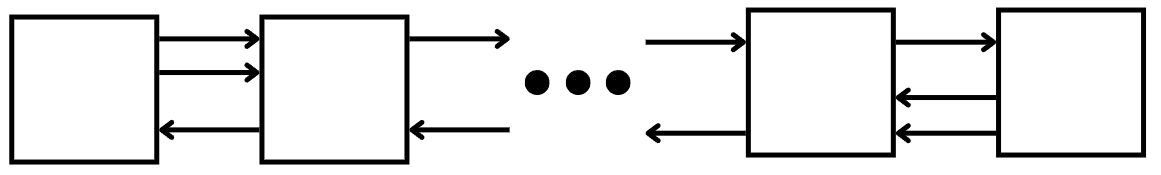
\includegraphics[width=\textwidth]{img/bReflexiva.png}
		\caption{Condición de frontera reflexiva}
		\label{fig:B_reflexiva}
	\end{subfigure}
	
	\caption{Condiciones de frontera con dos vecinos. La figura \ref{fig:B_reflectiva} muestra que las células en la frontera son vecinas entre sí, mientras que la figura \ref{fig:B_reflexiva} indica que las células que están al lado de las células de la frontera pueden tener múltiples relaciones de vecindad.}
	\label{fig:fronteras_adicionales}
\end{figure}

\section{Regla local}

Sea $\mathcal{S}$ el conjunto de estados y $m = |\mathcal{N}|$ el número de vecinos. La función de transición o regla local se define como 
\[
\mathcal{R}: \mathcal{S}^m \to \mathcal{S}
\] 
donde $\mathcal{R}$ asigna un nuevo estado a cada célula en función de los estados de sus $m$ vecinos (incluyéndose a sí misma si aplica).

Para autómatas celulares unidimensionales, dado un rango arbitrario $r$, la regla puede ser escrita como:
\[
\sigma_{i}(t + 1) = \mathcal{R}(\sigma_{i-r}(t), \sigma_{i-r+1} (t), \dots, \sigma_{i}(t), \dots, \sigma_{i+r} (t)), \; \mathcal{R}:  S^{2r + 1} \to S
\]
Donde el radio $r$ especifica el tamaño de la vecindad para cada célula (la vecindad es de tamaño $2r + 1$ como se muestra en la figura \ref{fig:N_wolfram}), la cual puede adquirir un valor $k$.

Un ejemplo de regla local es el juego de la vida \cite{lifewiki_life}. En este caso, el conjunto de estados es binario $\mathcal{S} = \{ 0, 1 \}$, donde $0$ representa células muertas y $1$ las vivas. La regla de transición realiza el siguiente mapeo:
\[
\mathcal{R}: \{ 0, 1 \}^9 \to \{ 0, 1\}
\]
Ya que la vecindad de Moore en 2D involucra 8 vecinos más la propia célula, es decir, $m = 9$. 

El juego de la vida sigue las siguientes tres reglas:

\begin{itemize}
	
	\item \textbf{Nacimiento}: Una célula muerta en el tiempo $t$ nace en el tiempo $t + 1$ si tiene exactamente tres vecinos vivos en el tiempo $t$.
	\item \textbf{Muerte}: Una célula viva en el tiempo $t$ muere en $t + 1$ por:
	\begin{itemize}
		\item Sobrepoblación; si hay más de tres vecinos vivos en $t$.
		\item Soledad: si hay menos de dos vecinos vivos en $t$.
	\end{itemize}
	\item \textbf{Supervivencia}: Una célula viva en el tiempo $t$ se mantiene viva en $t + 1$ si tiene dos o tres vecinos vivos en $t$.	 
\end{itemize}

Esta se conoce como regla semitotalística, ya que la transición depende de la suma de los valores en la vecindad, pero distingue entre diferentes posiciones, como el centro y los bordes \cite{genaro2022_semitotalistic}.

Por otro lado, una regla es totalística si la transición depende únicamente de la suma de los estados en todos los vecinos, sin distinguir posiciones \cite{weisstein2002_totalistic}. Para un autómata celular unidimensional con $|\mathcal{S}| = 3$ estados y radio $r = 1$, solo hay $(|\mathcal{S}|-1) |\mathcal{N}|+1 = (2-1) \cdot 3 + 1 = 4$ posibles valores de suma.

Finalmente, una regla local es arbitraria si distingue las posiciones de cada elemento en la vecindad. Cabe mencionar que las reglas arbitrarias contienen todas las posibles combinaciones de reglas, incluyendo las semitotalísticas, las cuales incluyen a su vez las totalísticas:
\[
	\mathcal{R}_{\text{totalísticas}} \subset \mathcal{R}_{\text{semitotalísticas}} \subset \mathcal{R}_{\text{arbitrarias}}
\]
El objetivo de las reglas semitotalísticas y totalísticas será entonces simplificar ciertos comportamientos.

La configuración dada para el autómata celular elemental considera $k = 2$ (es decir, $\sigma_i \in \{0, 1\}$), un radio $r = 1$ ($|\mathcal{N}| = 3$) y la regla $\mathcal{R}: \{0,1\}^3 \rightarrow \{0,1\}$ que se define como:
\[
\phi(\sigma_{i-1}(t), \sigma_{i}(t), \sigma_{i+1}(t))
\]
Esta dinámica está dada por las posibles configuraciones que las tres células adyacentes pueden adquirir en el tiempo $t$. Podemos encontrar $k^{|\mathcal{N}|} = 2^3 = 8$ patrones posibles en la vecindad, número correspondiente a la combinatoria de dos estados en tres posiciones. Cada vez que encontremos un patrón, podemos asignarle un nuevo estado a $\sigma_i(t + 1)$ ($\{ 0, 1 \}$), por lo que el número total de reglas asciende a $k^{k^{|\mathcal{N}|}} = 2^8 = 256$, como se muestra en la tabla \ref{tab:ECA_evolucion}.

\begin{table}
	
	\centering
	
	\begin{tabular}{c c c c c c c c} 
		
		111 & 110 & 101 & 100 & 011 & 010 & 001 & 000 \\
		
		$\downarrow$ & $\downarrow$ & $\downarrow$ & $\downarrow$ & $\downarrow$ & $\downarrow$ & $\downarrow$ & $\downarrow$ \\
		
		$\{ 0, 1 \}$ & $\{ 0, 1 \}$ & $\{ 0, 1 \}$ & $\{ 0, 1 \}$ & $\{ 0, 1 \}$ & $\{ 0, 1 \}$ & $\{ 0, 1 \}$ & $\{ 0, 1 \}$ 
		
	\end{tabular}
	
	\caption{Cada posible combinación de tres células puede adquirir uno de dos valores. Cuando la célula evaluada encaja en este patrón, su valor cambia al establecido por la regla. Este conjunto de 256 reglas se le conoce como autómata celular elemental.}
	
	\label{tab:ECA_evolucion}
	
\end{table}

Estas reglas se pueden representar de forma tabular y también como un número decimal. La tabla \ref{tab:ECA_rules} muestra la asociación entre la forma tabular y la regla decimal.

Nótese que la regla decimal solo aplica cuando las condiciones son las mismas. Es decir, cuando el número de vecinos $|\mathcal{N}|$ y estados $|\mathcal{S}|$ son invariantes; a cada regla se le puede asociar un entero único, pero dos reglas que difieren en vecindad o estados pueden compartir el número decimal. Por ejemplo, considerando la regla $10$ con $|\mathcal{N}| = 2$ y $|\mathcal{S}| = 2$ es $1010$, la cual es completamente diferente cuando $|\mathcal{N}| = 3$ y $|S| = 2$, lo que da como resultado $ 000000101$.

\begin{table}
	
	\centering
	
	\begin{tabular}{c | c c c c c c c c | c} 
		
		\textbf{Binario} &111 & 110 & 101 & 100 & 011 & 010 & 001 & 000 & \multirow{3}{*}{\textbf{regla}} \\ 
		
		\textbf{Decimal} & 7 & 6 & 5 & 4 & 3 & 2 & 1 & 0 & \\ 
		
		\textbf{Valor} & $2^7$ & $2^6$ & $2^5$ & $2^4$ & $2^3$ & $2^2$ & $2^1$ & $2^0$ & \\ \hline
		
		& 0 &  0 &  0 &  0 &  0 &  0 &  0 &  0 & 0 \\
		
		& 0 &  0 &  0 &  0 &  0 &  0 &  0 &  1 & 1 \\
		
		& \multicolumn{8}{c|}{\vdots} & \vdots \\ 
		
		& 0 &  0 &  0 &  1 &  1 &  1 &  1 &  0 & 30 \\
		
		& \multicolumn{8}{c|}{\vdots} & \vdots \\ 
		
		& 0 &  1 &  1 &  0 &  1 &  1 &  1 &  0 & 110 \\
		
		& \multicolumn{8}{c|}{\vdots} & \vdots \\ 
		
		& 1 &  1 &  1 &  1 &  1 &  1 &  1 &  1 & 255 
		
	\end{tabular}
	
	\caption{Los valores binarios representan las posibles configuraciones de estados que pueden aparecer en el espacio, cada uno asociado a un valor decimal, y el valor es la potencia asociada a esa combinación. Para convertir la regla tabular en la decimal, solo es necesario convertir el número binario.} 
	\label{tab:ECA_rules}
\end{table}

\section{Ejemplos}

\subsection{John Von Neumann}

El matemático y físico John von Neumann (1903-1957) fue uno de los pioneros en el estudio de los autómatas celulares, especialmente en lo que atañe a la reproducción automática y la universalidad computacional. En su obra póstuma, \textit{Theory of Self-Reproducing Automata}, presentó un modelo de autómata celular bidimensional diseñado para construir máquinas autorreplicantes. 

A continuación se presentan los principales elementos de su autómata celular, adaptados al formato de definición formal de este tipo de autómata:

\begin{itemize}
	
	\item \textbf{Espacio celular:} Von Neumann definió un espacio bidimensional como una cuadrícula regular de celdas, idealmente infinita.
	
	\item \textbf{Estados:} En su versión original, cada célula podía adoptar uno de 29 estados posibles que permiten distinguir células en reposo, células en transmisión de “señal”, células constructoras, etc. 

	\item \textbf{Vecindad:} Utiliza la vecindad que más tarde se denominaría ``vecindad de von Neumann''  \cite{weisstein2002_neumann}.
	
	\item \textbf{Función de transición:} Todas las células actualizan su estado de forma síncrona, de acuerdo con una regla común que depende del estado actual de la propia célula y de los estados de sus vecinos. En el modelo de von Neumann, esta regla está diseñada de modo que permita que ciertas configuraciones de células funcionen como un constructor universal capaz de autorreplicarse.
	
\end{itemize}

Su objetivo era demostrar de manera formal que se puede crear un autómata celular que se reproduzca sin fin y que, además, pueda hacer construcción universal dentro de ese sistema celular \cite{neumann1966_ca, wikipedia2016_ca}. 

\subsection{El juego de la vida}

El juego de la vida es un autómata celular propuesto por el matemático John Horton Conway en 1970. Consiste en una cuadrícula de celdas que pueden estar en uno de dos estados posibles: vivas o muertas. A lo largo del tiempo, las celdas evolucionan de acuerdo con un conjunto de reglas locales que determinan su supervivencia, muerte o nacimiento, en función del número de vecinos vivos que posean \cite{thoma2020_life}.

Siguiendo la definición formal de un autómata celular, el \textit{Juego de la Vida} se caracteriza por los siguientes elementos:

\begin{itemize}
	\item \textbf{Espacio celular}: Se define sobre una cuadrícula bidimensional regular, teóricamente infinita. 
	\item \textbf{Estados}: Cada célula puede encontrarse en un estado $\{ \text{muerto}, \text{vivo} \}$, representados comúnmente como $\{0, 1\}$.
	
	\item \textbf{Vecindad}: Se utiliza una vecindad de Moore semitotalística, la cual incluye las ocho celdas adyacentes a la célula central.
	
	\item \textbf{Función de transición}: El estado futuro de cada célula depende de su estado actual y del número de vecinos vivos, siguiendo las reglas:
	
	\begin{itemize}
		\item Una célula viva sobrevive cuando tiene dos o tres vecinos vivos.  
		\item Una célula viva con más de tres vecinos vivos muere por sobrepoblación.  
		\item Una célula viva que tiene menos de dos vecinos vivos muere por soledad.  
		\item Una célula muerta con exactamente tres vecinos vivos renace.  
	\end{itemize}
	
\end{itemize}
Estas reglas pueden modificarse para crear variantes del autómata, cambiando las condiciones de nacimiento o supervivencia. En \cite{lifewiki_life} se analizan distintas funciones de transición y configuraciones espaciales.

Una notación común es \textit{Birth/Survival}, que especifica los números de vecinos vivos requeridos para cada caso. El juego de la vida tradicional corresponde a la configuración $B3/S23$: una célula muerta nace con tres vecinos vivos, y una viva sobrevive si tiene dos o tres vecinos vivos \cite{lifewiki_life}.

Dentro de este sistema emergen patrones característicos, que se agrupan en tres categorías principales:

\begin{itemize}
	\item \textbf{Naturaleza muerta}: Estructuras estáticas que permanecen invariantes en el tiempo.  
	\begin{figure}[H]
		\centering
		\begin{subfigure}[b]{0.18\textwidth}
			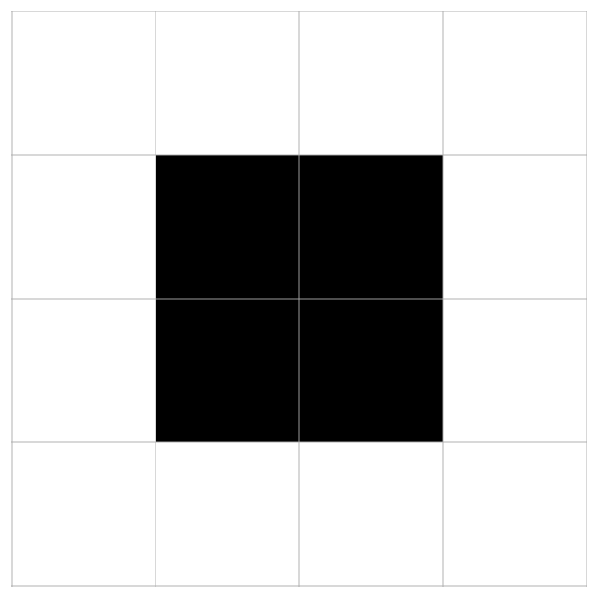
\includegraphics[width=\textwidth]{img/sl_block.png}
			\caption{\textit{Block}}
			\label{fig:block}
		\end{subfigure}
		\begin{subfigure}[b]{0.18\textwidth}
			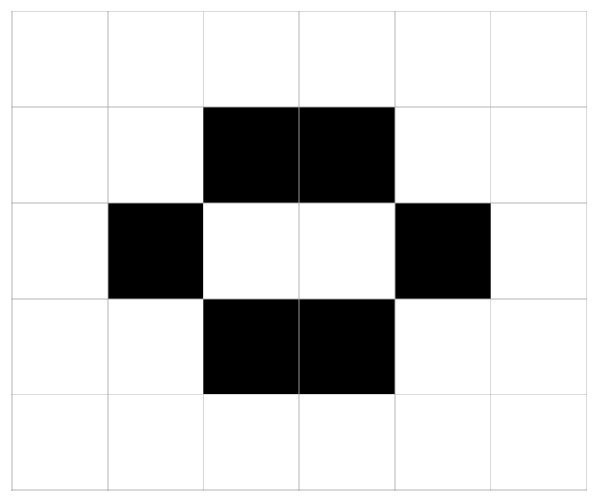
\includegraphics[width=\textwidth]{img/sl_beehive.png}
			\caption{\textit{Beehive}}
			\label{fig:beehive}
		\end{subfigure}
		\begin{subfigure}[b]{0.18\textwidth}
			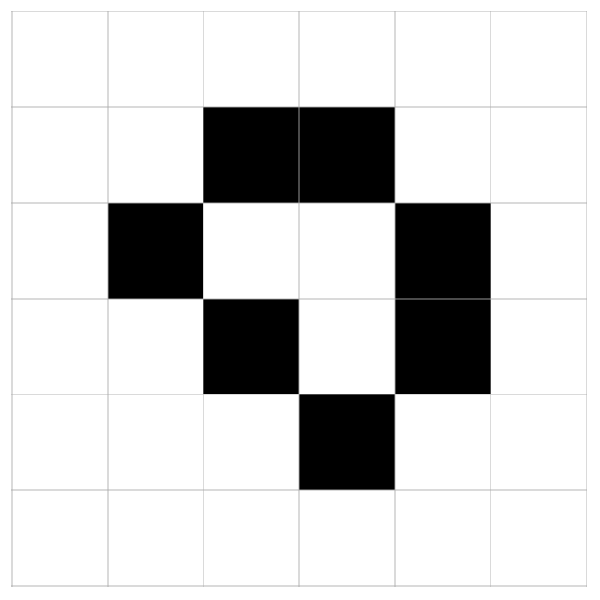
\includegraphics[width=\textwidth]{img/sl_loaf.png}
			\caption{\textit{Loaf}}
			\label{fig:loaf}
		\end{subfigure}
		\caption{Ejemplos de configuraciones de naturaleza muerta.}
		\label{fig:still_life}
	\end{figure}
	\item \textbf{Osciladores}: Patrones que repiten su configuración después de un número finito de iteraciones, manteniendo su posición en la cuadrícula.
	\begin{figure}[H]
		\centering
		\begin{subfigure}[b]{0.18\textwidth}
			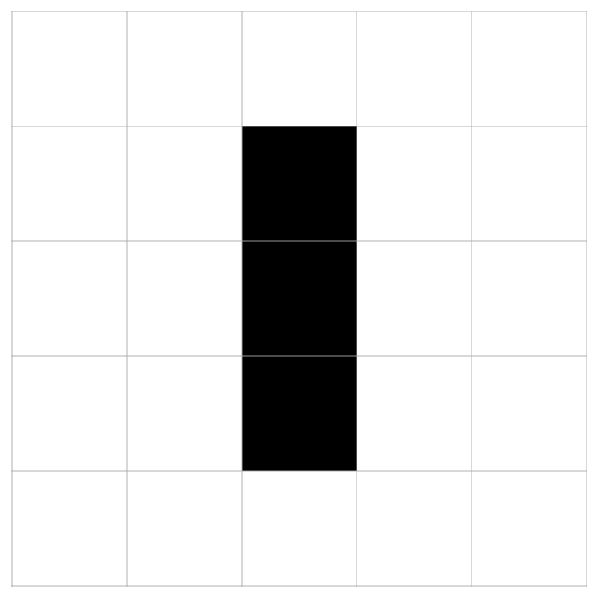
\includegraphics[width=\textwidth]{img/o_blinker_1.png}
		\end{subfigure}
		\begin{subfigure}[b]{0.18\textwidth}
			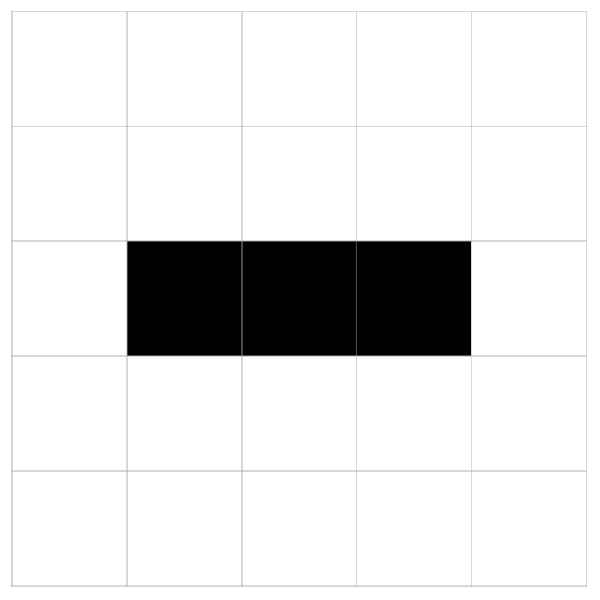
\includegraphics[width=\textwidth]{img/o_blinker_2.png}
		\end{subfigure}
		\caption{\textit{Blinker}.}
		\label{fig:blinker}
	\end{figure}
	\begin{figure}[H]
		\centering
		\begin{subfigure}[b]{0.18\textwidth}
			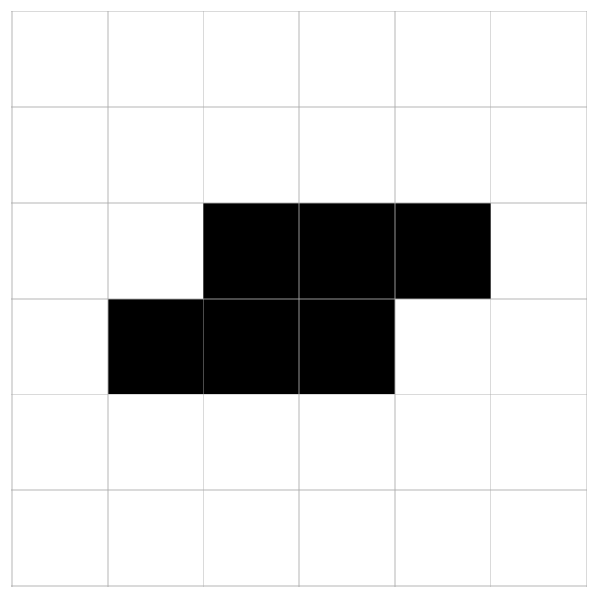
\includegraphics[width=\textwidth]{img/o_toad_1.png}
		\end{subfigure}
		\begin{subfigure}[b]{0.18\textwidth}
			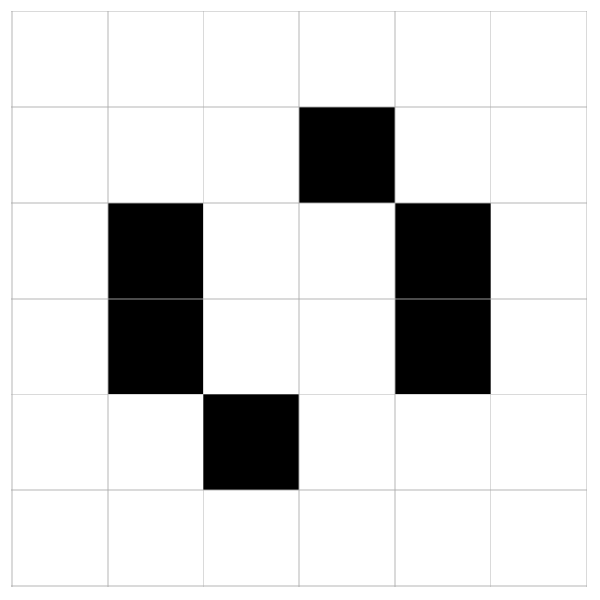
\includegraphics[width=\textwidth]{img/o_toad_2.png}
		\end{subfigure}
		\caption{\textit{Toad}.}
		\label{fig:toad}
	\end{figure}
	\item \textbf{Naves espaciales}: Son osciladores que, además de repetir su patrón, se desplazan por el espacio celular.  
	\begin{figure}[H]
		\centering
		\begin{subfigure}[b]{0.18\textwidth}
			
\includegraphics[width=\textwidth]{img/glider_1.png}
		\end{subfigure}
		\begin{subfigure}[b]{0.18\textwidth}
			
\includegraphics[width=\textwidth]{img/glider_2.png}
		\end{subfigure}
		\begin{subfigure}[b]{0.18\textwidth}
			
\includegraphics[width=\textwidth]{img/glider_3.png}
		\end{subfigure}
		\begin{subfigure}[b]{0.18\textwidth}
			
\includegraphics[width=\textwidth]{img/glider_4.png}
		\end{subfigure}
		\begin{subfigure}[b]{0.18\textwidth}
			
\includegraphics[width=\textwidth]{img/glider_5.png}
		\end{subfigure}
		\caption{\textit{Glider}.}
		\label{fig:glider}
	\end{figure}
\end{itemize}

Paul Rendell \cite{sipper2017_rendell_life} demostró que, a partir de una configuración inicial apropiada, el \textit{Juego de la Vida} es Turing completo, es decir, tiene la capacidad de realizar cualquier cálculo computable mediante la simulación de una máquina de Turing. La figura \ref{fig:conway_turing} muestra la configuración inicial del autómata celular diseñado por Paul Rendell.

\begin{figure}[!htbp]
	
	\centering
	
	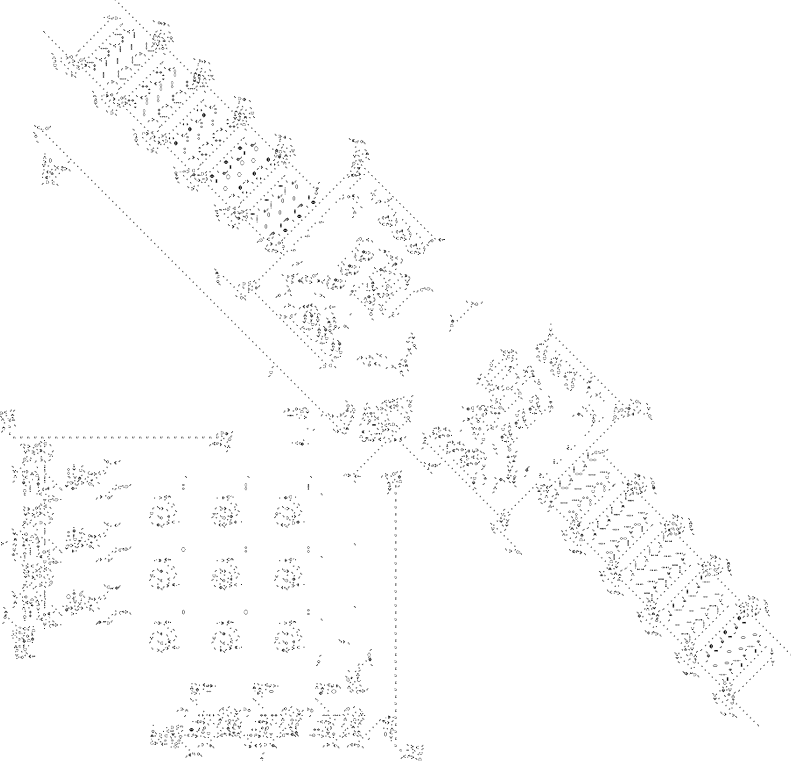
\includegraphics[width=0.85\textwidth]{img/gol_turing.png}
	
	\caption{Máquina de Turing implementada en el \textit{Juego de la Vida} \cite{rendell2000_turing_life}.}
	\label{fig:conway_turing}
\end{figure}

Debido a su naturaleza semitotalística, la vecindad puede dividirse en dos conjuntos, y con ello determinar el número de posibles estados que puede adoptar cada uno:

\begin{table}[!htbp] 
	
	\centering 
	
	\begin{tabular}{c|c|c}
		
		\hline \textbf{Vecindad} & \textbf{Estados} & \textbf{Total} \\ \hline 
		
		Frontera & $\{ 0,1,2,3,4,5,6,7,8 \}$ & 9 \\ 
		
		Centro & $\{ 0, 1 \}$ & 2 
		
	\end{tabular} 
	
\end{table}

Así, puede definirse un vector de 18 elementos que representa la función de transición, como se muestra en la tabla \ref{tab:life}.

\begin{table}[!htbp] 
	
	\centering 
	
	\begin{tabular}{c|c|c|c|c|c|c|c|c|c|c|c|c|c|c|c|c|c|c} 
		
		\hline 
		
		Frontera & 8& 7 & 6 & 5 & 4 & 3 & 2 & 1 & 0 & 8 &7 & 6 & 5 & 4 & 3 & 2 &1 &0 \\ 
		
		Centro & 1& 1& 1& 1& 1& 1& 1& 1& 1& 0& 0&0&0&0&0&0&0&0 \\ \hline 
		
		$B3/S23$ & 0 & 0 & 0 & 0 & 0 & 1 & 1 & 0 & 0 & 0 & 0 & 0 & 0 & 0 & 1 & 0 & 0 & 0 
		
		\\ \hline 
		
	\end{tabular}
	
	\caption{Representación binaria de la regla $B3/S23$.} 
	
	\label{tab:life} 
	
\end{table}

De manera general, el tamaño del vector que define una regla semitotalística puede calcularse mediante la ecuación \ref{eq:semitotalistica}. En este caso, dicho vector tiene tamaño 18, por lo que existen $|\mathcal{S}|^{18} = 2^{18} = 262,144$ posibles reglas.

\begin{equation}
	\prod_{i = 0}^{n} (|\mathcal{S}| - 1)(|n|) + 1, \quad \forall n \in \mathcal{N}
	\label{eq:semitotalistica}
\end{equation}

\subsection{Autómata celular elemental}

Stephen Wolfram propuso una versión más simple de los autómatas celulares, llamada autómata celular elemental. En esta versión, se disminuye la dimensionalidad del espacio celular y, por lo tanto, se reduce el tamaño de la vecindad. A continuación se detallan sus características según la definición formal de autómata celular:

\begin{itemize}
	
	\item \textbf{Espacio celular}: Está formado por una cadena unidimensional de celdas dispuestas linealmente.
	\item \textbf{Estados}: Cada célula puede encontrarse en uno de dos estados posibles, $\{0, 1\}$.
	\item \textbf{Vecindad}: Se define mediante un radio $r$ que determina cuántas celdas adyacentes influyen en la evolución de cada célula. En el caso del autómata celular elemental, el radio es $r = 1$, por lo que la vecindad está compuesta por la célula central y un vecino a cada lado.
	\item \textbf{Función de transición}: Wolfram no propuso una única regla de evolución, sino el conjunto completo de funciones de transición posibles bajo estas condiciones.
\end{itemize}

Dado que cada célula considera tres posiciones (la propia y sus dos vecinas) y cada una puede tener dos posibles estados, existen $2^3 = 8$ combinaciones de vecindad. Por tanto, el número total de reglas posibles es $2^{8} = 256$.

Wolfram asignó a cada una de estas funciones un número entero entre 0 y 255, conocido como número de regla, que identifica de forma unívoca el comportamiento del autómata. Además, propuso una clasificación de las reglas en cuatro categorías, según los patrones que emergen durante su evolución temporal (estas clases se detallan en la siguiente sección).

A continuación, se presentan tres reglas representativas por su relevancia teórica y sus propiedades computacionales.

\begin{itemize}
	
	\item \textbf{Regla 30}: La Regla 30 pertenece a la clase de comportamiento caótico. A partir de una configuración inicial simple, genera patrones altamente complejos y aparentemente aleatorios \cite{weisstein2002_rule30} como se muestra en las figuras \ref{fig:regla_30}.

	Esta regla plantea tres interrogantes fundamentales sobre la naturaleza del caos y la computabilidad:
	
	\begin{enumerate}
		\item ¿La columna central permanece no periódica a lo largo del tiempo?
		\item ¿Existe equilibrio estadístico entre los estados vivos y muertos?
		\item ¿Es posible calcular el estado de la célula central en el paso $n$ en tiempo $O(n)$?
	\end{enumerate}
	
	\begin{figure}[!htbp]
		\centering
		\begin{subfigure}[b]{0.75\textwidth}
			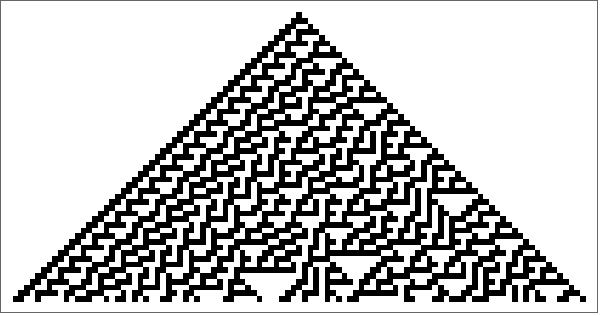
\includegraphics[width=\textwidth]{img/r30a.png}
			\caption{50 evoluciones.}
			\label{fig:30_1}
		\end{subfigure}
		\begin{subfigure}[b]{0.75\textwidth}
			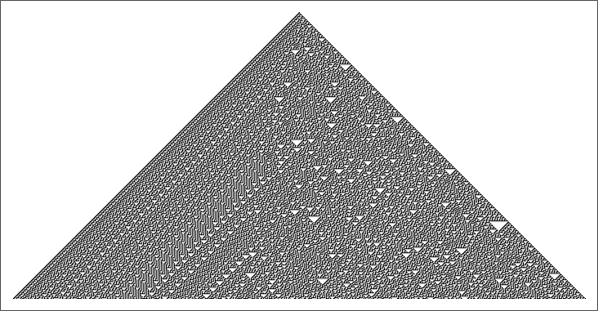
\includegraphics[width=\textwidth]{img/r30b.png}
			\caption{350 evoluciones.}
			\label{fig:30_2}
		\end{subfigure}
		\begin{subfigure}[b]{0.75\textwidth}
			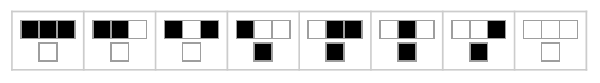
\includegraphics[width=\textwidth]{img/r30.png}
			\caption{Función de transición}
			\label{fig:30_rule}
		\end{subfigure}
		\caption{Evolución de la regla 30}
		\label{fig:regla_30}
	\end{figure}
	
	\item \textbf{Regla 110}: La Regla 110 exhibe un comportamiento mixto: combina regiones periódicas y caóticas que interactúan entre sí de manera compleja. A partir de una única célula activa, genera estructuras móviles y patrones que pueden coexistir en el tiempo \cite{weisstein2002_rule110}.
	
	Lo más notable de esta regla es su universalidad computacional. Wolfram y Matthew Cook demostraron que la Regla 110 es Turing completa, es decir, capaz de simular cualquier máquina de Turing y, por tanto, realizar cualquier cómputo posible en un sistema discreto determinista \cite{weisstein2002_rule110}. Su evolución se muestra en las figuras \ref{fig:regla_110}.
	
	\begin{figure}[!htbp]
		\centering
		\begin{subfigure}[b]{0.75\textwidth}
			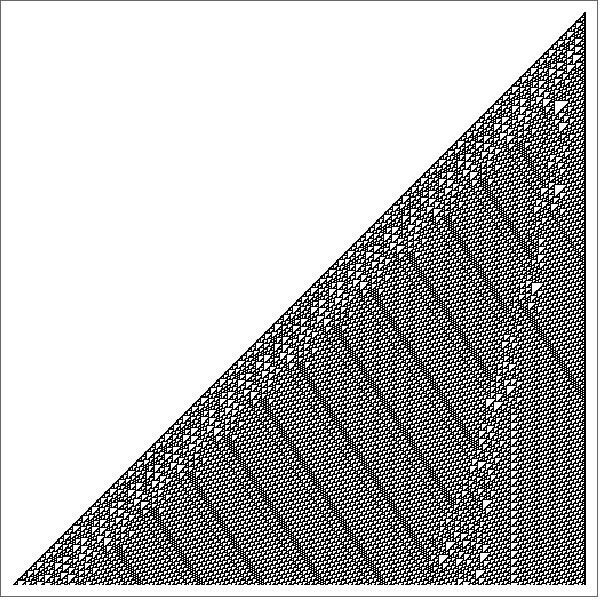
\includegraphics[width=\textwidth]{img/r110a.png}
			\caption{500 evoluciones.}
			\label{fig:110_1}
		\end{subfigure}
		\begin{subfigure}[b]{0.75\textwidth}
			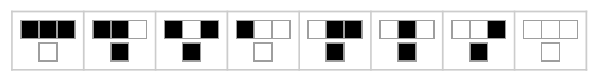
\includegraphics[width=\textwidth]{img/r110.png}
			\caption{Función de transición}
			\label{fig:110_rule}
		\end{subfigure}
		\caption{Evolución de la regla 110}
		\label{fig:regla_110}
	\end{figure}
	
	\item \textbf{Regla 90}: La Regla 90 se distingue por generar estructuras fractales. Iniciando desde una única célula activa, produce el conocido triángulo de Sierpinski como se muestra en la figura \ref{fig:regla_90}, el cual es un patrón autosimilar que aparece en múltiples sistemas naturales y matemáticos \cite{weisstein2002_rule90}.
	
	\begin{figure}[!htbp]
		\centering
		\begin{subfigure}[b]{0.75\textwidth}
			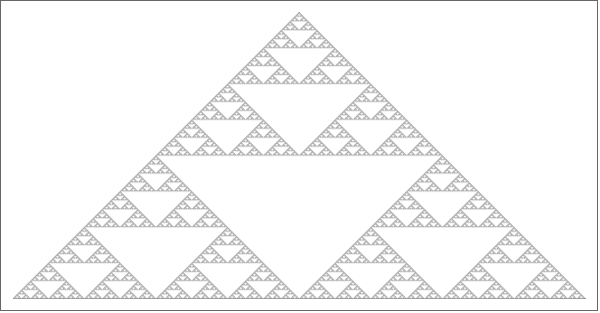
\includegraphics[width=\textwidth]{img/r90a.png}
			\caption{1025 evoluciones.}
			\label{fig:90_1}
		\end{subfigure}
		\begin{subfigure}[b]{0.75\textwidth}
			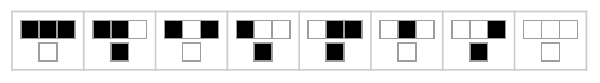
\includegraphics[width=\textwidth]{img/r90.png}
			\caption{Función de transición}
			\label{fig:90_rule}
		\end{subfigure}
		\caption{Evolución de la regla 90}
		\label{fig:regla_90}
	\end{figure}
\end{itemize}

\section{Clasificación}

Los autómatas celulares elementales fueron utilizados por diferentes autores por representar la máxima simplicidad y mínima configuración que un autómata puede adquirir y que tenga un amplio rango de comportamientos. Múltiples autores han intentado definir una clasificación; a continuación se muestran algunas clasificaciones propuestas por diferentes autores. 

Stephen Wolfram realiza una clasificación basada en el comportamiento que exhiben ciertas reglas y que es inherente a la configuración inicial. Es por esto que define las siguientes clases de comportamiento, ilustradas en la figura \ref{fig:clasificacion}:

\begin{enumerate}[label=W\Roman*]
	\item Evolucionan a un estado uniforme. 
	\item Evolucionan a estados cíclicos aislados.
	\item Evolucionan en comportamientos caóticos.
	\item Evolucionan en estados complejos aislados.
\end{enumerate}

\begin{figure}[!htbp]
	\centering
	\begin{subfigure}[b]{0.45\textwidth}
		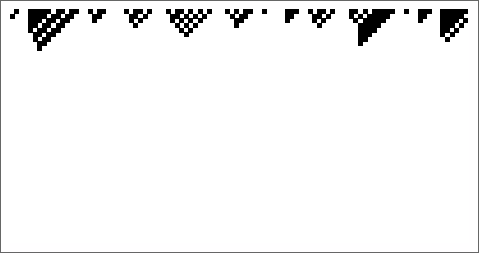
\includegraphics[width=\textwidth]{img/c1.png}
		\caption{Clase I: Regla 168}
		\label{fig:c1}
	\end{subfigure}
	\begin{subfigure}[b]{0.45\textwidth}
		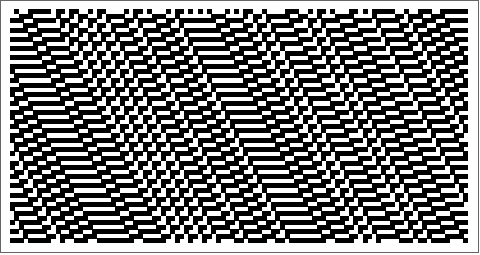
\includegraphics[width=\textwidth]{img/c2.png}
		\caption{Clase II: Regla 27}
		\label{fig:c2}
	\end{subfigure}
	\begin{subfigure}[b]{0.45\textwidth}
		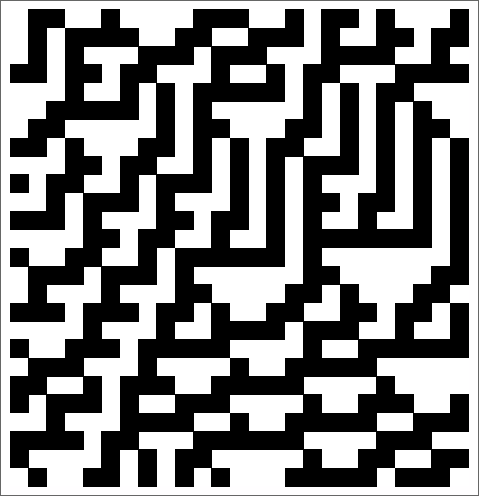
\includegraphics[width=\textwidth]{img/c3.png}
		\caption{Clase III: Regla 105}
		\label{fig:c3}
	\end{subfigure}
	\begin{subfigure}[b]{0.45\textwidth}
		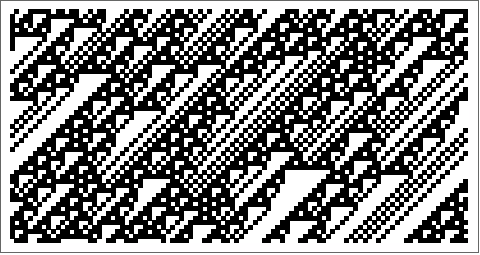
\includegraphics[width=\textwidth]{img/c4.png}
		\caption{Clase IV: Regla 106}
		\label{fig:c4}
	\end{subfigure}
	\caption{Clasificación de Wolfram. Las figuras evolucionan 50 pasos con la misma configuración inicial y con condición de frontera cíclica.}
	
	\label{fig:clasificacion}
	

\end{figure}

\begin{comment}
	
En la tabla \ref{tab:class_wolfram} se muestra la relación de reglas del autómata celular elemental. 

\begin{table}
	\centering
	\begin{tabular}{c|c|p{0.5\textwidth}}
		Tipo & Total & Reglas \\ \hline
		Clase I & 8 & 0, 8, 32, 40, 128, 136, 160, 168 \\ 
		Clase II & 65 & 1, 2, 3, 4, 5, 6, 7, 9, 10, 11, 12, 13, 14, 15, 19, 23,
		24, 25, 26, 27, 28, 29, 33, 34, 35, 36, 37, 38, 42,
		43, 44, 46, 50, 51, 56, 57, 58, 62, 72, 73, 74, 76,
		77, 78, 94, 104, 108, 130, 132, 134, 138, 140, 142,
		152, 154, 156, 162, 164, 170, 172, 178, 184, 200,
		204, 232. \\ 
		Clase III & 11 & 18, 22, 30, 45, 60, 90, 105, 122, 126, 146, 150. \\ 
		Clase IV & 4 &  41, 54, 106, 110.
	\end{tabular}
	\caption{Relación de reglas del autómata celular elemental con la clasificación de Wolfram.}
	\label{tab:class_wolfram}
\end{table}
\end{comment}

Sin embargo, existen reglas bajo diferentes configuraciones que pueden pertenecer a múltiples clases o, en el peor de los casos, no pertenecen a ninguna de ellas \cite{genaro2000_campo_promedio}. 

Li y Packard ofrecen otra clasificación que considera seis clases para categorizar el comportamiento dinámico de los autómatas celulares \cite{genaro2013_class}:
\begin{enumerate}[label*=LP\Roman*]
	\item La regla evoluciona a un estado homogéneo donde todas las células adquieren el mismo valor.
	\item Evoluciona hasta una configuración estática no necesariamente homogénea.
	\item Reglas con un periodo igual a dos.
	\item Reglas con un periodo de $L$.
	\item Evolucionan a estructuras caóticas.
	\item Conduce a estructuras largas y estructuras complejas.
\end{enumerate}

Por otro lado, Culick y Yu \cite{genaro2013_class, culik1988_class} proponen una clasificación que sigue las siguientes limitaciones: 

\begin{itemize}
	\item Esta clasificación es para autómatas celulares no totalísticos. 
	\item Cada clase es un subconjunto de la siguiente clase.
\end{itemize}

\begin{enumerate}[label*=CY \Roman*]
	\item Un autómata celular es de clase I si existe un estado estable $s \in \mathcal{S}$ tal que todas las configuraciones finitas evolucionan a una configuración homogénea de $s$.
	
	Es decir, dada cualquier configuración inicial en un autómata celular finito, todas las células adquieren el estado $s$ tras cierto número de pasos evolutivos. Esto se aplica a todas las finitas configuraciones iniciales.
	
	\item Un autómata celular es de clase II si existe un estado estable $s \in \mathcal{S}$ tal que se repite a $n$ pasos evolutivos.
	
	Esto implica que la evolución se repite cada $n$ número de pasos ($\sigma(t) = \sigma(t + n)$). Resulta evidente que la clase I está contenida en la clase II, haciendo que $n = 1$, lo que implica un periodo de uno.
	
	Una clasificación es $s$-finita si solo difiere del estado estable en una región finita.
	
	\item Un autómata celular es de clase III si existe un estado estable $s \in \mathcal{S}$ tal que para cualquier par de configuraciones $s$-finitas $C_1$ y $C_2$, es decidible si $C_1$ evoluciona a $C_2$.
	
	Es decir, si podemos determinar en tiempo finito si el CA evoluciona de $C_1$ a $C_2$, entonces pertenece a clase III. En caso contrario, pertenece a la clase IV, la cual contiene a todos los autómatas celulares \cite{culik1988_class}.
	
	\item Todos los autómatas celulares pertenecen a la clase IV.	
\end{enumerate}

\section{Extensiones y cambios de la definición}

Otra clasificación considera extensiones o modificaciones en la definición que alteran el comportamiento del autómata celular. A continuación, se describen algunas de estas extensiones para el modelado de sistemas complejos. 

\begin{itemize}
	
	\item \textbf{Autómatas celulares en grafos}: Amplían la idea de la estructura de red clásica al permitir que las vecindades no sean iguales: cada célula puede tener un número diferente de vecinos. Esta flexibilidad los hace adecuados para modelar fenómenos sobre grafos, como redes sociales o flujos en infraestructura. Sin embargo, diseñar manualmente las reglas de transición en estos entornos es una tarea compleja, lo que ha motivado propuestas como los autómatas celulares neuronales en grafos, que permiten aprender dichas reglas automáticamente \cite{grattarola2021_gca}.
	
	\item \textbf{Autómatas celulares probabilísticos}: Estos extienden el modelo clásico al incorporar reglas de transición estocásticas. En vez de una evolución que sigue un camino fijo, los estados futuros dependen de probabilidades que se ven afectadas por el entorno. Esto ayuda a entender la incertidumbre, el ruido y los comportamientos que surgen de manera inesperada. Son especialmente útiles para simular dinámicas como propagación de epidemias o sistemas sociales, donde los mecanismos de transición no siempre están completamente definidos \cite{gacs2024_pca}.
	
	\item \textbf{Autómatas celulares no homogéneos}: Permiten que diferentes células tengan diferentes funciones de transición. Para esto, se utilizan dos planos llamados ``plano de datos'', el cual contiene la evolución del sistema; y ``plano de control'', el cual define las reglas de transición para cada célula. Esto permite estudiar el comportamiento y la interacción entre diferentes reglas que comparten espacio \cite{hartman1987_ihca}.
	
	\item \textbf{Autómatas celulares continuos}: Son autómatas celulares que pueden ser continuos en los estados, en el tiempo y en el espacio \cite{Wolfram2002_nks}:
	
	\begin{itemize}
		\item Los estados continuos adquieren valores reales y no solo enteros.
		
		\item El tiempo continuo se define mediante una función que determina el intervalo de espera para actualizar la célula en función de su estado actual.
		
		\item El espacio continuo se obtiene al asignar diferentes pesos a las células dentro de la vecindad \cite{becker2023_cca}.
	\end{itemize}
\end{itemize}

Estas variantes no son exclusivas y además han ampliado el uso de los autómatas celulares. Sin embargo, un problema que se repite es definir correctamente las reglas de transición para lograr un fenómeno específico. Este desafío ha llevado a la creación de autómatas celulares neuronales. En estos, la función de transición no se define de manera clara, sino que se aprende a través de una red neuronal artificial. Pero antes de adentrarse en la definición, es necesario comprender qué son las redes neuronales.

\clearpage
	
	\chapter{Marco teórico: Inteligencia artificial y redes neuronales}

Las redes neuronales artificiales son una herramienta de inteligencia artificial inspirada en el pensamiento humano, más específicamente, en cómo un conjunto de neuronas interconectadas comparten información para realizar inferencias. 	

Las redes neuronales tienen su origen en 1943, donde McCulloch y Pitts propusieron un modelo que establecería las bases del perceptrón. Posteriormente, en 1957, Rosenblatt formalizó su implementación computacional, pero no fue hasta los años ochenta donde tuvo un impacto en su implementación gracias al surgimiento de la retropropagación y de las redes recurrentes \cite{matich2001_ann}.

Las redes neuronales artificiales son un conjunto de neuronas o módulos computacionales interconectados que realizan cálculos y transmiten información para llevar a cabo una operación, imitando el comportamiento del cerebro.

Sin embargo, para entender este modelo, es necesario tener los fundamentos de inteligencia artificial y la clasificación de aprendizaje supervisado. Es por esto que en este capítulo, se describen términos como inteligencia artificial, aprendizaje supervisado, la composición, estructura y comportamiento de las redes neuronales y algunos tipos de ellas. 

\section{Inteligencia artificial}

La inteligencia artificial fue definida por primera vez por John McCarthy en 1955 como \textit{la ciencia e ingeniería de hacer máquinas inteligentes} \cite{Manning2020_ai}. Es un término que ha ido evolucionando a lo largo de los años y con diferentes interpretaciones. Para el objetivo de esta investigación y siguiendo a \cite{Manning2020_ai, google2025_ai, mccarthy2007_ai}, se sigue la siguiente definición:

\begin{definition}
	La inteligencia artificial es la ciencia que utiliza modelos computacionales para crear sistemas capaces de realizar tareas que, si fueran hechas por humanos, requerirían inteligencia.
\end{definition}

Una de las ramas de la inteligencia artificial es el aprendizaje automático, el cual se centra en desarrollar sistemas con la capacidad de aprender en función de los datos \cite{oracle2025_ml}. Esto permite reconocer patrones y realizar predicciones a partir de grandes cantidades de datos \cite{google_ml}.

Por lo que, con base en \cite{oracle2025_ml, ibm_ml} podemos definir al aprendizaje automático como:

\begin{definition}
	El aprendizaje automático es la disciplina que permite a las computadoras mejorar su desempeño en una tarea mediante la experiencia con datos, sin necesidad de instrucciones explícitas.
\end{definition}

Esta tecnología funciona trabajando a través del entrenamiento de algoritmos en conjuntos de datos para conseguir un resultado esperado. Es el proceso de optimizar el modelo para que pueda predecir la respuesta correcta. A mayor calidad en los datos de entrenamiento, mayor precisión se tendrá en el modelo \cite{google_ml}.

El entrenamiento se refiere al proceso de enseñarle a un modelo de inteligencia artificial a realizar una o varias tareas mediante la exposición a grandes cantidades de datos \cite{main2023_training}. Este proceso facilita a los humanos el proceso de análisis de extensos volúmenes, especialmente en la era actual, donde se generan más datos que nunca en la historia \cite{oracle2024_big_data}.

Dentro del aprendizaje automático se definen tres métodos en cómo una computadora puede aprender. Estos métodos son aprendizaje supervisado, no supervisado y por refuerzo.

\begin{itemize}
	\item El aprendizaje supervisado se caracteriza por el uso de conjuntos de datos etiquetados para entrenar algoritmos que clasifiquen datos o predigan resultados con precisión. Durante el proceso de entrenamiento, el modelo recibe entradas junto con las salidas correctas, lo que le permite al modelo ajustar sus parámetros hasta que sea capaz de realizar predicciones precisas sobre nuevos datos \cite{ibm_ml}. 
	
	\item El aprendizaje no supervisado, a diferencia del supervisado, no necesita de un conjunto de datos etiquetados generados por el ser humano. Este tipo de aprendizaje puede descubrir patrones y estadísticas sin ninguna orientación o instrucción explícita \cite{google_u_ml}. 
	
	\item El aprendizaje por refuerzo busca imitar la forma de aprendizaje humana de prueba y error. Este tipo de aprendizaje permite a las máquinas aprender a tomar decisiones y mejorar sus resultados con base en los errores cometidos \cite{aws_r_ml}.
	
\end{itemize}

IBM \cite{ibm_ml} menciona algunos de los algoritmos más comunes de aprendizaje automático:

\begin{enumerate}
	\item \textbf{Regresión lineal:} Predice valores numéricos, con base en una relación lineal entre diferentes valores.
	
	\item \textbf{Agrupación en clústeres:} Identifican patrones en los datos y los agrupan en centroides.
	
	\item \textbf{Árboles de decisión:} Utilizan una secuencia ramificada de decisiones vinculadas que se representan con un diagrama de árbol.
	
	\item \textbf{Redes neuronales:} Simulan el funcionamiento del cerebro humano, con un gran número de nodos de procesamiento conectados entre sí, llamados neuronas.
\end{enumerate}

Las redes neuronales presentan ventajas que pueden llegar a agilizar y optimizar recursos de las organizaciones que lo implementan \cite{adobe_ml}: mejora la productividad, reduce el error humano, mejora la disponibilidad de servicios, reduce tareas repetitivas, descubre patrones ocultos a simple vista, entre otros.

Para comprender cómo las redes neuronales logran estas capacidades, es necesario explorar primero los fundamentos que inspiraron el desarrollo. En particular su diseño es una abstracción de las neuronas biológicas, cuya estructura y funcionamiento ofrecen una analogía para el procesamiento de la información.

\section{Neurona biológica}

Las neuronas son células especializadas del sistema nervioso cuyo objetivo es recibir, procesar y transmitir información por medio de señales químicas y eléctricas \cite{navarra_neurona, bordoli2023_neurona}. 

Cada neurona se compone (principalmente) de tres elementos, como se muestra en la figura \ref{fig:neurona}: 

\begin{itemize}
	
	\item Las dendritas, que reciben señales provenientes de otras neuronas.
	
	\item El núcleo o cuerpo, que integra las señales provenientes de las dendritas y produce una nueva señal eléctrica.
	
	\item El axón, el cual conduce la señal producida por el cuerpo hacia otras neuronas haciendo sinapsis, es decir, transmite la señal de una célula a otra.
	
\end{itemize}

\begin{figure}[!htbp]
	
	\centering
	
	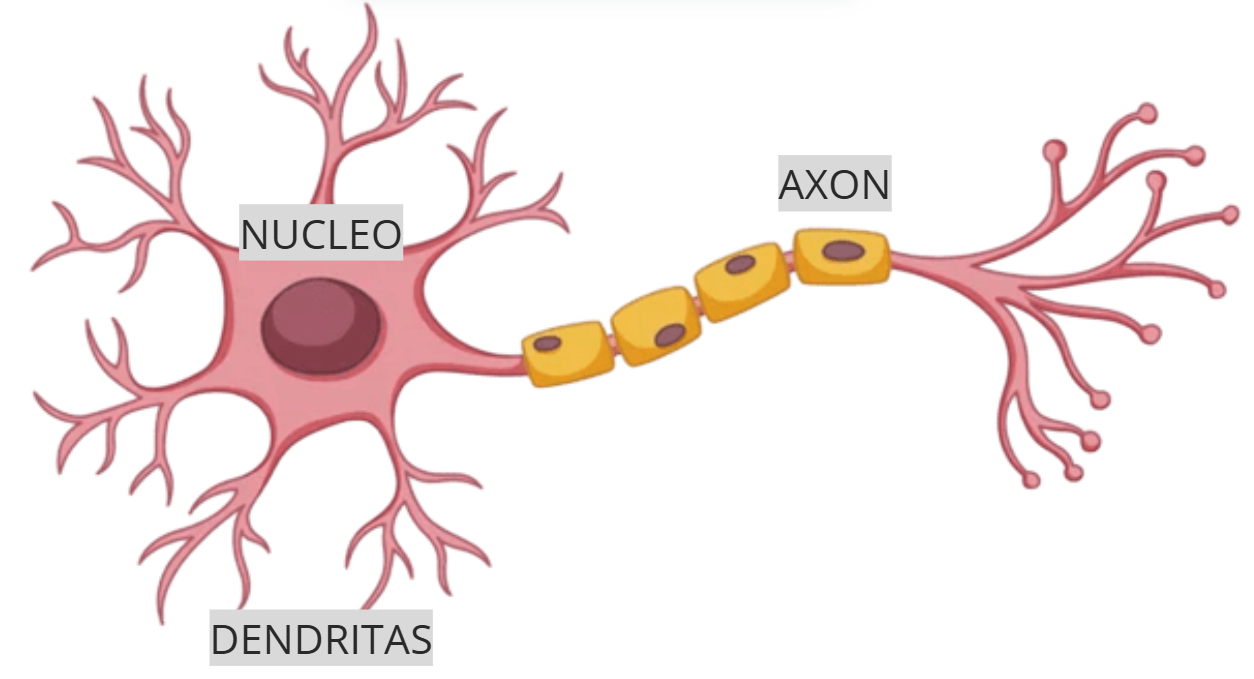
\includegraphics[width=0.6\linewidth]{img/neurona.png}
	
	\caption{Representación de una neurona \cite{brgfx_neurona}. Se encuentran señaladas las dendritas, el núcleo y el axón, encargado de recibir, procesar y transmitir la información, respectivamente.}
	
	\label{fig:neurona}
	
\end{figure}

Las redes neuronales naturales son un sistema de neuronas que permite el procesamiento cerebral de la información; son altamente complejas, no lineales y con procesamiento en paralelo. 

\section{Neurona artificial} 

La neurona artificial se considera como una unidad de procesamiento de información \cite{navarra_neurona}. Sigue la misma estructura del modelo biológico con algunas consideraciones adicionales, como lo marcan \cite{navarra_neurona, Mhatre2020_neurona_artificial, leon2017_neurona_artificial}:

\begin{itemize}
	
	\item Las dendritas equivalen al conjunto de datos de entrada. Sin embargo, no toda la información tiene la misma relevancia; para esto se le asigna a cada entrada un peso sináptico.
	
	\item El cuerpo se sustituye por dos funciones: (1) una función de agregación que combina todos los datos de entrada (generalmente es una combinación lineal entre las entradas y los pesos sinápticos) y (2) una función de activación que determina si la neurona está activa y en qué grado. 
\end{itemize}

La cual se suele representar como en la figura \ref{fig:neurona_artificial}.

\begin{figure}[!htbp]
	
	\centering
	
	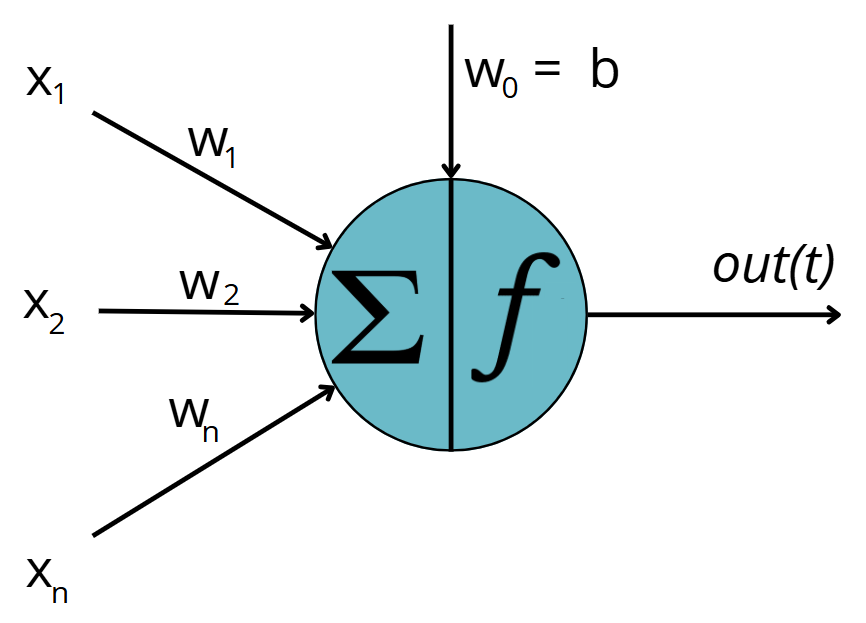
\includegraphics[width=0.6\linewidth]{img/neurona_artificial.png}
	
	\caption{Representación gráfica de una neurona artificial. Contiene las entradas ($x_1, x_2, \dots, x_n$), los pesos sinápticos ($w_1, w_2, \dots, w_n$), el sesgo ($w_0$ o $b$), la función de agregación ($\Sigma$), la función de activación ($f$) y la salida.}
	\label{fig:neurona_artificial}
	
\end{figure}
\begin{definition}
	Una neurona artificial es una función $f: \mathbb{R}^n \to \mathbb{R}$ dada por:
	\[
	f(x) = \phi (\omega (X, W, b))
	\]
	donde:
	\begin{itemize}
		
		\item $X = \{x_1, x_2, \dots, x_n\} \in \mathbb{R}^n$ es el conjunto de datos que recibe cada neurona.
		\item $W = \{ w_1, w_2, \dots, w_n \} \in \mathbb{R}^n$ es el conjunto de pesos sinápticos que indican la importancia de cada entrada.
		
		\item $b$ o $w_0 \in \mathbb{R}$ es un sesgo que desplaza la función de activación y controla el umbral de aceptación.
		
		\item $\omega(X,W,b)$ es una función de agregación $\omega: \mathbb{R}^n \to \mathbb{R}$ que combina las entradas. Usualmente se define como una combinación lineal:
		\[
		\omega(X,W,b) = \sum_{i = 1}^{n} w_i x_i + b
		\]
		\item $\phi(\omega(X,W,b))$ es la función de activación $\phi: \mathbb{R} \to \mathbb{R}$ que transforma $\omega(X,W,b)$ en una salida activada.
	\end{itemize}

\end{definition}

Además de la combinación lineal, la función de agregación puede adoptar otras formas, como el máximo, el mínimo o combinaciones lógicas (AND, OR) en redes con entradas binarias. No obstante, la suma ponderada continúa siendo la más utilizada en aplicaciones prácticas \cite{matich2001_ann}.

La función de activación es la que determina el valor de salida de cada neurona. Este valor, normalmente, se encuentra acotado dentro de un rango específico (como $[0, 1]$ o $[-1, 1]$) para normalizar el comportamiento de la red \cite{google_activacion}. Además, su naturaleza no lineal es fundamental para que el modelo pueda aproximar funciones complejas y resolver problemas que no son linealmente separables.

\section{Redes neuronales}

Una neurona únicamente puede realizar una operación. Para aumentar la capacidad de entender patrones más complejos, es necesario añadir múltiples neuronas interconectadas, lo que se conoce como red neuronal artificial \cite{aws_ann}. Esta puede definirse como un grafo dirigido \cite{tech2019_ann}.

\begin{definition}
	Una red neuronal artificial es un grafo dirigido $G = (V, E)$ donde cada nodo $v \in V$ representa una neurona y cada arista $(u, v) \in E$ transporta la salida $y_u$ desde $u$ hasta $v$ ponderada por el peso $w_{uv}$. 
	
	Existe un conjunto de nodos de entrada $X \subseteq V$ que reciben los datos iniciales y un conjunto de nodos de salida $T \subseteq V$ cuya activación final representa la salida de la red.
	
\end{definition}

Aunque la topología de la red puede ser arbitraria, en la práctica las redes se organizan en tres conjuntos de capas. Esto se muestra en la figura \ref{fig:ann_multicapa}, las cuales son (1) una de entrada que recibe los datos, (2) una o varias ocultas y (3) una de salida que devuelve el resultado. Adicionalmente, suelen diseñarse redes neuronales completamente conectadas, es decir, todas las neuronas tienen una relación con todas las de la siguiente capa, pero no es una restricción \cite{ibm2021_ann}. 

\begin{figure}[!htbp]
	\centering
	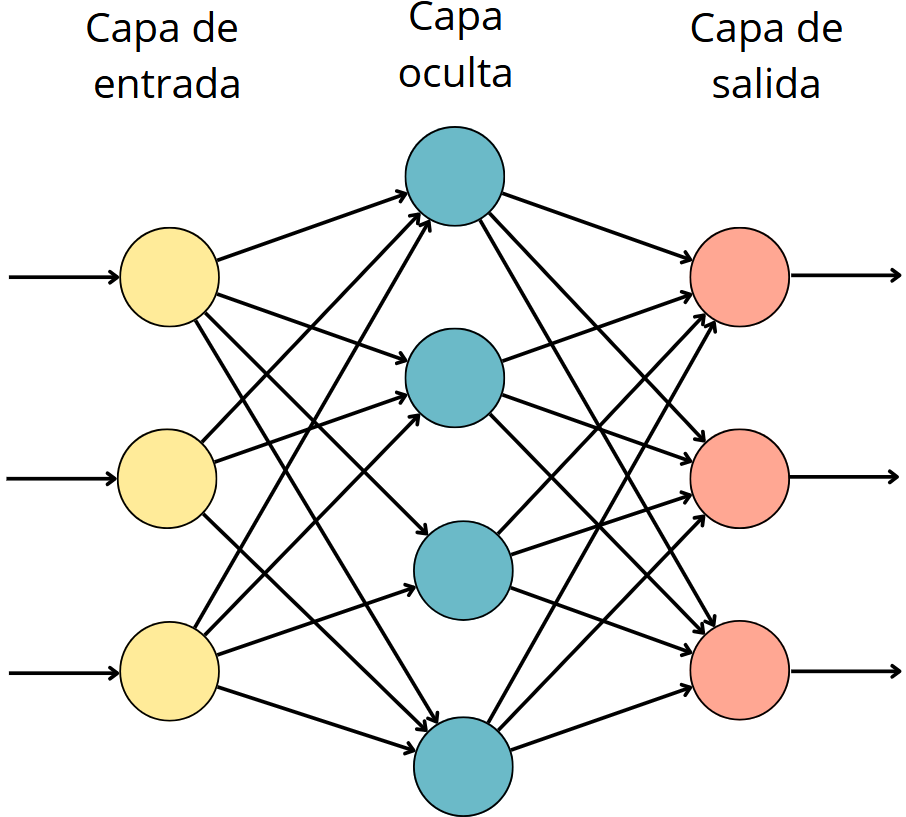
\includegraphics[width=0.5\textwidth]{img/ANN_multicapa.png}
	\caption{Red neuronal de tres capas: tres entradas, una capa oculta y tres salidas.}
	\label{fig:ann_multicapa}
\end{figure}

La red en su conjunto implementa una función parametrizada.
\[F_\theta: \mathbb{R}^n \to \mathbb{R}^m\] 

donde $n$ es el número de datos de entrada, $m$ el número de datos de salida y $\theta$ el conjunto de parámetros entrenables. El entrenamiento de una red neuronal consiste en ajustar $\theta$.

Por lo que se puede concluir con la definición de \cite{matich2001_ann}, la cual dice que
\begin{definition}
	Una red neuronal es una función $F_\theta: \mathbb{R}^n \to \mathbb{R}^m$ donde $\theta = \{ w_{uv}, b_v : (u, v) \in E, v \in V \}$ es el conjunto de parámetros entrenables.
\end{definition}

\subsection{Funciones de activación}

La capacidad de $F_\theta$ para modelar relaciones no lineales depende de las funciones de activación aplicadas en cada nodo $v$. Sin la función de activación, la red neuronal podría definirse únicamente como una función lineal.

En esta sección se presentan las funciones de activación más comunes utilizadas en redes neuronales. Para cada función se muestra su definición matemática, una breve descripción de su comportamiento práctico y una figura ilustrativa.

\subsubsection{Binary step (escalón binario)}

La función escalón binario se define por partes:
\[
f(x) =
\begin{cases}
	1 & \text{si } x \ge 0,\\[4pt]
	0 & \text{si } x < 0.
\end{cases}
\]
Produce salidas discretas (0/1) y fue utilizada en perceptrones tempranos como función de decisión. No es diferenciable en el punto de umbral y su derivada es nula en casi todas partes, por lo que no es adecuada para entrenamiento mediante gradiente (backpropagation). Aun así, se usa conceptualmente para tomar decisiones discretas o como capa de postprocesado/umbral en modelos ya entrenados.
\begin{figure}[!htbp]
	\centering
	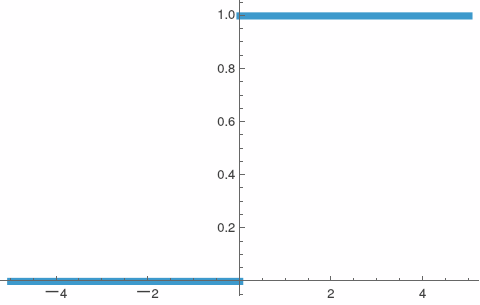
\includegraphics[width=0.5\textwidth]{img/binary.png}
	\caption{Función de activación escalón binario.}
	\label{fig:binary}
\end{figure}

\subsubsection{Lineal}
La función lineal (o identidad) se define como:
\[
f(x) = ax + b \quad \lor \quad f(x)=x.
\]
Produce una salida proporcional a la entrada y mantiene la linealidad en la red. Se utiliza principalmente en la capa de salida para tareas de regresión donde se requiere predecir valores continuos. No es adecuada para capas ocultas cuando se desea que la red aprenda transformaciones no lineales.
\begin{figure}[!htbp]
	\centering
	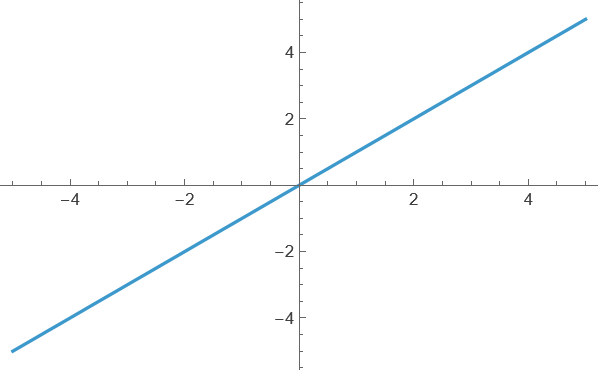
\includegraphics[width=0.5\textwidth]{img/lineal.png}
	\caption{Función de activación lineal.}
	\label{fig:linear}
\end{figure}

\subsubsection{Sigmoide}

La función sigmoide logística se define como:
\[
\sigma(x) = \frac{1}{1 + e^{-x}}.
\]
Tiene la propiedad de:
\[
\sigma'(x) = \sigma(x)\,(1 - \sigma(x)).
\]
Comprime la entrada en el intervalo $(0,1)$, por lo que es apropiada para modelar probabilidades y se ha usado históricamente en la salida de clasificadores binarios. Sufre saturación cuando los valores son grandes, lo que provoca gradientes pequeños (esto se llama el problema del gradiente desvanecido) y una salida que no está centrada (es positiva). Por eso, en las capas ocultas modernas, a menudo se reemplaza por ReLU o tanh.
\begin{figure}[!htbp]
	\centering
	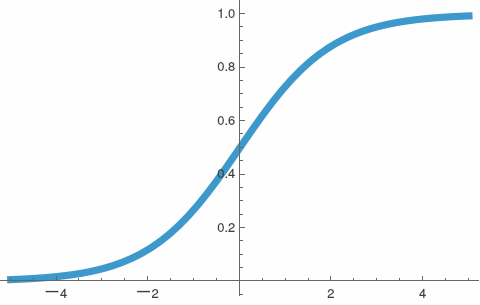
\includegraphics[width=0.5\textwidth]{img/sigmoid.png}
	\caption{Función de activación sigmoide.}
	\label{fig:sigmoid}
\end{figure}

\subsubsection{tanh (hiperbólica)}

La tangente hiperbólica se define como:
\[
\tanh(x) = \frac{e^{x} - e^{-x}}{e^{x} + e^{-x}}.
\]
Su rango es $(-1, 1)$ y su derivada puede expresarse en función de sí misma.  

Es una versión centrada en cero de la sigmoide, lo que facilita el aprendizaje (gradientes con medias cercanas a cero). Se usa en capas ocultas cuando se necesita una salida limitada y centrada. Era una opción común en problemas secuenciales y en redes neuronales tradicionales antes de que se popularizaran arquitecturas y funciones de activación más modernas.
\begin{figure}[!htbp]	
	\centering
	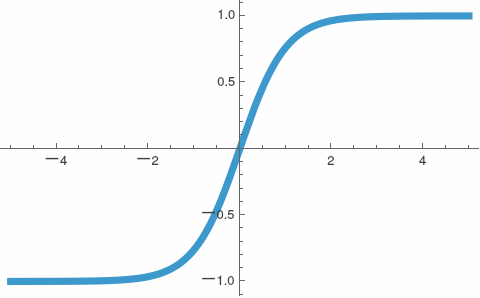
\includegraphics[width=0.5\textwidth]{img/tanh.png}
	\caption{Función de activación \texttt{tanh}.}
	\label{fig:tanh}
\end{figure}

\subsubsection{ReLU (Rectified Linear Unit)}

La función ReLU se define por partes:
\[
f(x) = \max(0, x).
\]
Activa linealmente las entradas positivas y pone a cero las negativas. Es sencillo y computacionalmente eficiente, favorece la esparcidad de activaciones y reduce en la práctica el problema del gradiente desvanecido en redes profundas. Muy utilizada en capas ocultas de arquitecturas modernas. Tiene la desventaja de poder provocar neuronas ``muertas'' (gradiente cero para entradas negativas), problema que funciones como Leaky ReLU intentan corregir.
\begin{figure}[!htbp]
	\centering
	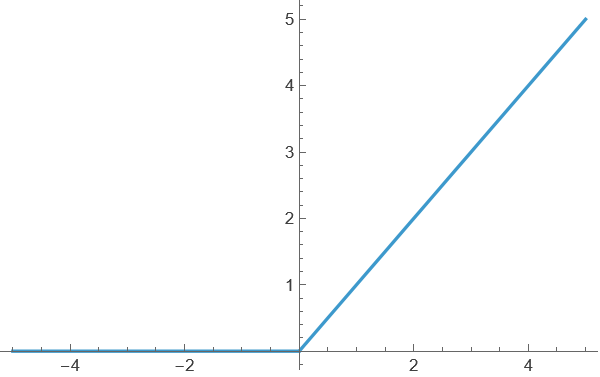
\includegraphics[width=0.5\textwidth]{img/relu.png}
	\caption{Función de activación ReLU.}
	\label{fig:relu}
\end{figure}

\subsection{Aprendizaje en redes neuronales}

Dada una red neuronal artificial con los parámetros entrenables totalmente configurados, es capaz de realizar su clasificación o predicción de manera correcta. Sin embargo, resulta imposible configurar estos pesos manualmente, por lo que requiere de un ``entrenamiento'' que ayude a definir los pesos sinápticos. A continuación se define la función de pérdida, optimización y entrenamiento, elementos necesarios para obtener esa configuración específica.

En los primeros modelos, la actualización de los pesos se realizaba a partir del error cuadrático del valor de activación. La regla de actualización se expresaba como:
\[
	\Delta w_j = - \alpha(c- a)x_j
\]
Donde $a$ representa la activación y $\alpha$ la tasa de aprendizaje. Este método permitió superar la no diferenciabilidad de la función escalón en los perceptrones originales \cite{matich2001_ann}.

\subsubsection{Función de pérdida}

La función de pérdida se usa para medir el rendimiento del modelo. Calcula la desviación que existe entre el valor predicho y el valor esperado. Esta función puede ser un escalar o un vector que permite aproximar la tasa de error para llegar a una solución óptima \cite{bergmann_funcion_perdida}. 

\begin{definition}
	
	Sea $F_\theta$ una red neuronal artificial y $ \mathcal{D} = \{ (x^{(i)}, y^{(i)}) \}_{i = 1}^n $ un conjunto de datos de entrenamiento donde $x^{(i)}$ es la entrada y $y^{(i)}$ es la salida esperada; una función de pérdida es un mapeo que tiene la siguiente forma: 
	\[
	\mathcal{L}: \mathbb{R}^m \times \mathbb{R}^m \to \mathbb{R}_{\geq 0}
	\]
	Tal que mide la discrepancia entre la predicción del modelo y la salida real:
	\[
	\mathcal{L} (F_\theta (x^{(i)}, y^{(i)}))
	\]
\end{definition}

Es importante que la función de pérdida sea diferenciable. El gradiente de la función de pérdida permite conocer la dirección hacia la cual debe moverse para disminuir la pérdida.

Las funciones de pérdida se pueden utilizar para regresión y para clasificación. La primera mide el error en valores continuos y se utiliza para estimar valores contables como el precio, tamaño y tiempo. La segunda mide los errores en valores discretos, como la clasificación o la categoría.

Distintas funciones de pérdida priorizan diferentes tipos de error; la elección de la función de pérdida dependerá de la tarea que se desea realizar. Además, la función de pérdida únicamente se aplica a una muestra; para una población de muestras, se utiliza la función de costo, que se define a continuación \cite{bergmann_funcion_perdida, ultralytics2025_funcion_perdida}:

\begin{definition}
	
	Sea $F_\theta$ una red neuronal artificial y $\mathcal{L}$ la función de pérdida; la función de costo es el promedio de las pérdidas:
	\[
	J(\theta) = \frac{1}{n} \sum_{i = 1}^{n} \mathcal{L}(F_\theta(x^{(i)}), y^{(i)})
	\]
\end{definition}

\subsubsection{Optimización}

El entrenamiento de una red consiste en ajustar los parámetros entrenables $\theta$ para minimizar la función de pérdida. La optimización consiste en resolver el problema de minimización dado por:
\[
\theta^* = \arg \min_{\theta} J(\theta)
\]
Esto se puede conseguir mediante diferentes técnicas, siendo el descenso del gradiente la más común. Este método actualiza los parámetros en la dirección opuesta al gradiente de la función de pérdida:
\[
\theta_{t + 1} = \theta_{(t)} - \eta  \nabla_\theta J(\theta^{(t)})
\]
donde $\eta >0$ es la tasa de aprendizaje. Una tasa de aprendizaje alta puede divergir en la solución, mientras que una tasa baja puede tener una convergencia lenta \cite{matich2001_ann}. 

En la práctica, es común iniciar el entrenamiento con una tasa de aprendizaje relativamente alta y luego reducirla gradualmente a medida que el modelo converge. También se suele incorporar un término de \textit{momentum }para acelerar la convergencia y reducir oscilaciones \cite{matich2001_ann}.

\subsubsection{Entrenamiento}

Antes del entrenamiento, las variables de entrada deben normalizarse para ajustarse al rango de activación de la red (por ejemplo, $[0,1]$ o $[-1,1]$). Este paso evita que una variable con valores grandes domine la función de agregación y mejora la estabilidad del entrenamiento. Es importante que la normalización preserve la distribución original de los datos y la proporción entre atributos \cite{matich2001_ann}.

Finalmente, el entrenamiento consiste en ajustar todos los parámetros $\theta = \{ W^{(l)}, b^{(l)}\}$ para minimizar la función de costos $J(\theta)$ en un conjunto de datos de entrenamiento. Este proceso se compone de las siguientes etapas:

\begin{enumerate}
	
	\item Se inicializan los parámetros, generalmente de forma aleatoria: $\theta_0 \sim \mathcal{D}_{init}$

	\item Se hace la propagación hacia adelante o \textit{forward pass}, es decir, para cada entrada $x^{(i)}$ se evalúa $\hat{y}^{(i)} = F_\theta(x^{(i)})$ 

	\item Se calcula la pérdida: $\mathcal{L}^{(i)} = \mathcal{L}(\hat{y}^{(i)}, y^{(i)})$
	
	\item Se calculan los gradientes propagando la información hacia atrás o \textit{backpropagation} utilizando la regla de la cadena.	
	\[
	\nabla_\theta J(\theta) = \frac{1}{N} \sum_{i = 1}^{N} \nabla_\theta \mathcal{L} (F_ \theta(x^{(i)}, y ^{(i)}))
	\]
	Se actualizan los parámetros mediante la función de optimización: $\theta_{t + 1} = \theta_{(t)} - \eta  \nabla_\theta \mathcal{L}(\theta^{(t)})$

	\item Se repite este proceso sobre un \textit{dataset} hasta la convergencia de la solución o hasta alcanzar un criterio de parada \cite{matich2001_ann}.
	
	Una vez entrenada la red, puede evaluarse la importancia relativa de las entradas mediante un análisis de sensibilidad. Este procedimiento consiste en:
	
	\begin{enumerate}
		\item Calcular el valor medio de cada entrada.
		\item Evaluar la salida de la red con todos los valores medios.
		\item Modificar una entrada a la vez (aumentándola o disminuyéndola) y medir el cambio en la salida.
		\item Repetir el proceso para cada variable de entrada.
	\end{enumerate}
	
	De esta manera, se identifica qué variables influyen más en el resultado, lo cual aporta interpretabilidad al modelo \cite{matich2001_ann}.
	
\end{enumerate}

La elección de la topología de la red, en particular el número de neuronas ocultas, suele determinarse empíricamente. Una regla práctica consiste en comenzar con un número de neuronas ocultas similar al número de entradas y ajustar a partir del rendimiento obtenido. Otras heurísticas recomiendan iniciar con el doble de nodos de entrada y reducir gradualmente si se detecta sobreajuste \cite{matich2001_ann}.

En resumen, el entrenamiento de la red neuronal es un proceso iterativo de optimización que consiste en:

\begin{enumerate}
	
	\item Propagar los datos de entrada por la red.
	
	\item Comparar la salida con el valor real usando una función de pérdida.
	
	\item Propagar el error hacia atrás permite obtener gradientes.
	
	\item Actualizar los parámetros con un algoritmo de optimización.
	
	\item Repetir hasta que el modelo aproxime adecuadamente la función deseada.
	
\end{enumerate}

\section{Tipos de redes neuronales}

Las redes neuronales pueden clasificarse atendiendo a diferentes criterios, ya sea por el número de capas, el tipo de conexiones, el grado de conectividad o la arquitectura general. En este trabajo se han seleccionado dos tipos principales, de manera enunciativa, mas no limitativa, que son especialmente relevantes para su eventual implementación en un autómata celular neuronal: las redes neuronales convolucionales y las recurrentes. La razón de esta elección es la siguiente:

Por un lado, las evoluciones de un autómata celular ocurren de forma secuencial en el tiempo, es decir, las entradas y salidas de la red corresponden a estados del espacio celular y, en algunos casos, las reglas pueden tener una relación temporal o reversible. De ahí que las redes recurrentes resulten particularmente apropiadas.

Por otro lado, como se explicará más adelante, se ha demostrado que los autómatas celulares y las redes neuronales convolucionales tienen algunas similitudes, especialmente porque el \textit{kernel} de la red convolucional es similar a la vecindad del autómata celular.

\subsection{Redes neuronales convolucionales}

Las redes neuronales convolucionales constituyen una clase de redes profundas cuya estructura está diseñada para explotar la topología de los datos que tienen forma de rejilla. Por ejemplo, imágenes en dos dimensiones.

Una red neuronal convolucional consta de una capa de entrada, varias capas ocultas (que pueden incluir capas de convolución, normalización, \textit{pooling}, activación, etc.) y una capa de salida.

Se asume un volumen de entrada con dimensiones $(H \times W \times C)$, es decir, altura $H$, anchura $W$ y $C$ canales (por ejemplo, RGB en imágenes). La red maneja este volumen usando filtros deslizantes. Aunque normalmente no se describen en términos de estados discretos de autómatas, se puede entender que cada neurona de una capa representa un estado continuo real (por ejemplo, una activación $a \in \mathbb{R}$).

El elemento clave es su operación de convolución: un filtro (o \textit{kernel}) de tamaño $k \times k$ se desliza sobre la entrada, compartiendo pesos y produciendo mapas de activación. Se puede ver como una vecindad local de la neurona que influye en su valor de activación que se aplica en cada capa de convolución:
\[
Y = f(X * K + b)
\]
Donde $X$ es el volumen de entrada, $K$ es el filtro (o filtros) de convolución, $b$ es el sesgo y $f$ es una función de activación. A continuación pueden seguir operaciones de \textit{pooling} y capas totalmente conectadas para producir la salida final \cite{amidi2025_cnn}.

Se aplica principalmente en clasificación de imágenes, segmentación, reconocimiento de video y procesamiento de audio. En el contexto de los autómatas celulares, se puede ver que el filtro de la red neuronal convolucional es similar a la vecindad del autómata. Esto permite entenderlo como una operación de actualización local que se repite en un espacio organizado, igual que en un autómata celular.

\subsection{Redes neuronales recurrentes}

Las redes neuronales recurrentes son un tipo de redes que tienen conexiones que vuelven sobre sí mismas. Esto permite que la información de momentos anteriores afecte el procesamiento que se está realizando en el presente.

Una red neuronal recurrente trabaja con una serie de entradas $(x_1, x_2, \dots, x_T)$ y genera una serie de salidas $(y_1, y_2, \dots, y_T)$. En cada momento, la red tiene un estado oculto $h_t$ que se actualiza de la siguiente manera:

\begin{gather*}
	h_t = f(W_{xh} x_t + W_{hh} h_{t-1} + b_h), \\
	y_t = g(W_{hy} h_t + b_y),
\end{gather*}

Donde $W_{xh}$, $W_{hh}$ y $W_{hy}$ son matrices de pesos, $b_h$ y $b_y$ son sesgos, y $f$, $g$ son funciones de activación.

La red funciona en una secuencia de tiempo, donde cada momento puede verse como una "capa virtual" o una repetición del autómata. En cada instante $t$, el estado oculto $h_t$ muestra la "memoria" o el contexto acumulado hasta ese momento.

La vecindad temporal está dada por la conexión de la unidad de tiempo $t$ con la anterior $t-1$ (y en variantes bidireccionales, también con $t+1$). Es decir, la salida de un paso se inserta como parte de la entrada del siguiente paso.

Como se mostró más arriba, la actualización recursiva del estado oculto actúa como la función de transición temporal de la red. La red integra información histórica para producir la salida en cada paso de tiempo.

Estas redes se utilizan frecuentemente en el procesamiento de lenguaje natural, reconocimiento de voz, series temporales, traducción automática y otras tareas en las que el orden temporal de los datos es esencial \cite{amidi2025_rnn}.

Dado que un autómata celular evoluciona en pasos discretos de tiempo y cada uno puede depender del estado previo del sistema, las redes neuronales recurrentes aportan un modelo natural para capturar dependencias temporales entre estados sucesivos del autómata. Esto resulta especialmente útil si la regla del autómata celular tiene memoria o se desea que aprenda dinámicas espacio-temporales.

En conclusión, mientras que las redes neuronales convolucionales capturan la estructura espacial y la vecindad local del sistema, las redes neuronales recurrentes modelan su evolución y persistencia temporal. La integración de ambas capacidades permite que un autómata celular neuronal no solo emule reglas estables, sino que aprenda dinámicas complejas a partir de datos, superando las limitaciones de las reglas de transición diseñadas manualmente.

\clearpage
	\chapter{Marco teórico: Autómatas celulares neuronales}

En los últimos años, los autómatas celulares neuronales surgieron como una extensión de los clásicos, con las capacidades de aprendizaje y generalización propias de las redes neuronales artificiales. Esta integración permite que la regla de transición, tradicionalmente fija, sea parametrizable y entrenable mediante técnicas de aprendizaje supervisado.

Las primeras aproximaciones copiaban el funcionamiento de un autómata celular usando una red neuronal convolucional \cite{gilpin2019_nca}. Este método fue dado a conocer por Mordvintsev  et al. \cite{mordvintsev2020_nca}, quienes entrenaron un modelo que aprende de dinámicas locales a partir de ejemplos. Como resultado, las interacciones locales básicas cumplen un objetivo en específico, mostrando propiedades de crecimiento, regeneración, autoorganización y morfogénesis.

Los autómatas celulares neuronales son entonces un tipo de autómatas celulares, pero cuya función de transición está definida como una red neuronal artificial. Retomando las definiciones previas, podemos decir entonces que:

\begin{definition}
	
	Un autómata celular es neuronal si la regla local $\mathcal{R}$ está dada como:
	\[
	\mathcal{R} = F_\theta: \mathbb{R}^{|\mathcal{N}|} \to \mathbb{R}^1
	\]
	donde:
	
	\begin{itemize}
		
		\item $F_\theta$ es una red neuronal parametrizada por $\theta$.
		
		\item $ \theta = \{ w_{uv}, b_v : (u, v) \in E, v \in V \}$ es el conjunto de parámetros entrenables.
		
		\item $\mathbb{R}^{|\mathcal{N}|}$ corresponde al espacio de entrada definido por la vecindad $\mathcal{N}$.
		
		\item $\mathbb{R}^1$ define el valor de salida que representa el nuevo estado de la célula central.
		
	\end{itemize}
	
\end{definition}

La figura \ref{fig:nca} muestra la relación existente entre estas dos tecnologías. En el paso $N$ se tiene una configuración bidimensional con vecindad de Neumann. El estado de cada elemento dentro de la vecindad funciona como valor de entrada para la red neuronal entrenada y devuelve un único resultado. Este resultado corresponde a la salida de la célula central, es decir, a la cual se le está aplicando.

\begin{figure}[!htbp]
	
	\centering
	
	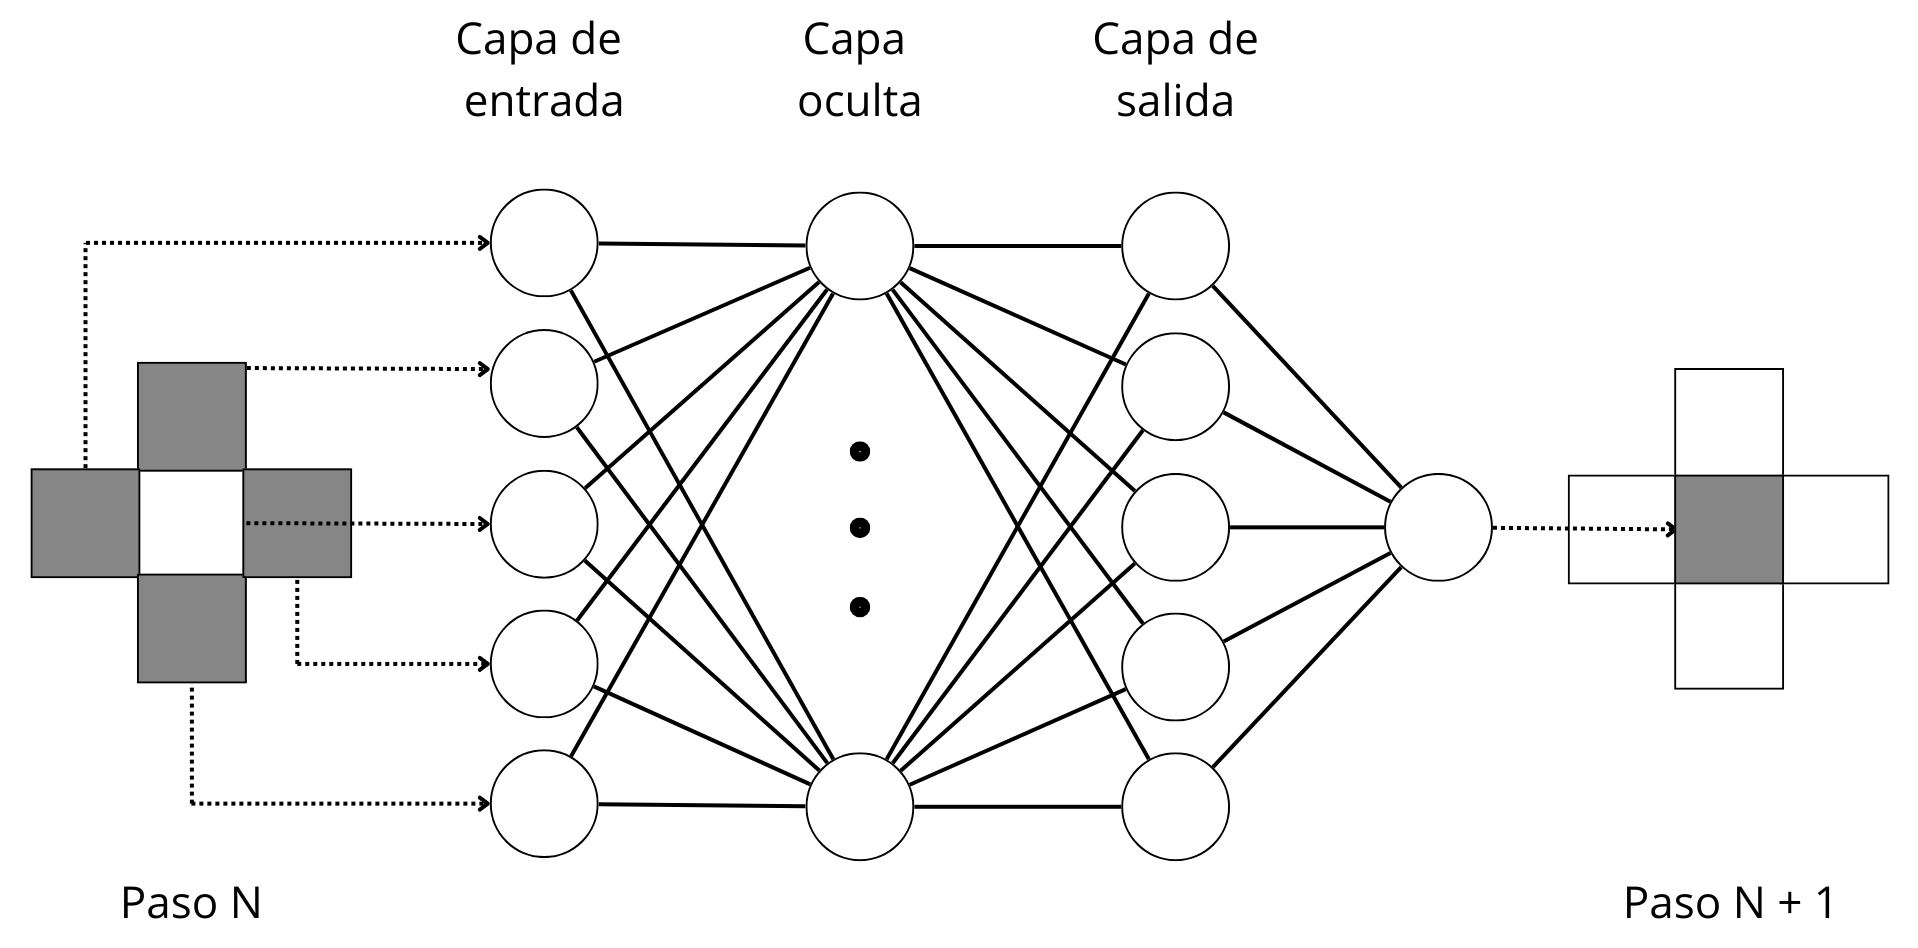
\includegraphics[width=0.8\textwidth]{img/NCA.png}
	
	\caption{Representación gráfica de la red neuronal.}
	
	\label{fig:nca}
	
\end{figure}

Cada célula aplica una misma red neuronal local $F_\theta$ sobre su vecindad inmediata. La entrada de la red consiste en los estados de las celdas dentro de la vecindad y la salida es el nuevo estado de la célula central. 

$F_\theta$ suele representarse como una red neuronal artificial convolucional que permite procesar localmente la información espacial preservando la estructura $D$-dimensional. 

A diferencia de los autómatas clásicos, donde las reglas son explícitas y definidas manualmente, los autómatas celulares neuronales aprenden sus reglas mediante un proceso de entrenamiento. Se establece un grupo de condiciones iniciales $X_0$ y un estado final $X^*$. Luego, la red $F_\theta$ se ajusta para reducir una función de pérdida $\mathcal{L}(X_T, X^*)$, que mide la diferencia entre la configuración obtenida después de $T$ pasos y el estado deseado. Este proceso puede expresarse como:
\[
\theta^* = \arg\min_\theta \mathcal{L}(F_\theta^{(T)}(X_0), X^*).
\]
Durante el entrenamiento, se emplean técnicas de retropropagación a través del tiempo y optimización por gradiente descendente. Esto permite que la red aprenda comportamientos dinámicos complejos, tales como el crecimiento morfológico, la regeneración parcial o la adaptación frente a perturbaciones.

Como las redes neuronales generan valores reales, se puede medir la tasa de error entre la predicción que hacen y el comportamiento real del sistema al usar la regla que han aprendido. Esta métrica de error se propone como base para el desarrollo del presente trabajo. Sin embargo, también se puede comparar la pérdida con otros elementos cercanos, ya que dos células pueden tener muchos vecinos en común, lo que podría explicar el error que se observa en la predicción.

Como se muestra a continuación, esta herramienta ha demostrado ser capaz de generar patrones autoorganizados y adaptativos sin necesidad de una programación explícita de reglas. Algunos ejemplos incluyen:

\begin{itemize}
	
	\item \textbf{Morfogénesis:} Crecimiento de formas y estructuras similares a organismos biológicos.
	
	\item \textbf{Regeneración:} Capacidad de reconstruir regiones dañadas o eliminadas de la configuración.
	
	\item \textbf{Modelado de sistemas complejos:} Simulación de fenómenos físicos, ecológicos o sociales mediante interacciones locales entrenables.
	
\end{itemize}

Esta mezcla de comportamiento que aparece por sí mismo y la habilidad de aprender hace que los autómatas celulares neuronales sean una herramienta muy útil para estudiar sistemas que se organizan solos y que se adaptan.

Los autómatas celulares neuronales surgen de la necesidad de definir funciones de transición más precisas que permitan mejorar la simulación de sistemas complejos, como por ejemplo la propagación del fuego. 

Consideremos un autómata celular bidimensional con tres posibles estados: $\{ materia \; viva, fuego, materia\; quemada \}$, una vecindad de Moore y una función de transición definida por las siguientes reglas: si una célula en estado de materia viva se encuentra adyacente a una célula en estado de fuego, entonces se quema; y si una célula en estado de fuego está rodeada principalmente de materia quemada, entonces se apaga.

Sin embargo, esta formulación que se basa en reglas claras es una simplificación excesiva que reduce la capacidad del modelo para imitar comportamientos que se ven en sistemas reales. Para superar esta limitación, los autómatas celulares neuronales incorporan mecanismos de aprendizaje automático que permiten definir la función de transición de manera adaptativa. 

En este enfoque, el autómata aprende a partir de ejemplos. Por ejemplo, secuencias de video que muestran la propagación del fuego, donde cada estado puede representarse mediante un color y cada célula corresponde a un píxel o conjunto de píxeles. De esta manera, la red neuronal subyacente aprende una función de transición capaz de imitar la dinámica del sistema complejo, ajustando sus parámetros a partir de los datos observados.

Adicionalmente, los autómatas celulares tradicionales suelen operar con configuraciones reducidas, es decir, con pocos estados, vecindades mínimas y reglas básicas, ya que el espacio de configuraciones crece exponencialmente al incrementar cualquiera de estos factores. Esta limitación dificulta modelar sistemas complejos presentes en la naturaleza, los cuales suelen involucrar múltiples variables e interacciones de alta dimensionalidad.

\section{Estado del arte, aplicaciones y líneas actuales de investigación}

Un primer avance en esta línea fue presentado por Gilpin \cite{gilpin2019_nca}, demostrando que una red neuronal convolucional puede aprender el comportamiento de un autómata celular clásico. Su estudio destaca que tanto los autómatas celulares como las redes neuronales convolucionales comparten dos propiedades fundamentales: (1) la actualización basada en una vecindad o \textit{kernel}, y (2) la aplicación simultánea de dicha función en todo el espacio.

En particular, Gilpin entrenó una red neuronal convolucional con un \textit{kernel} de $3 \times 3$ (mismo tamaño que la vecindad de Moore) para imitar el comportamiento del \textit{glider}\footnote{Una de las configuraciones más importantes por su capacidad de moverse en el espacio} en el Juego de la Vida de John Conway. Este trabajo estableció una conexión entre los autómatas celulares y las redes neuronales convolucionales, mostrando que estas redes artificiales pueden actuar como mecanismos de transición local aprendidos.

Posteriormente, esta línea de investigación fue extendida por Mordvintsev et al. \cite{mordvintsev2020_nca}, quienes exploraron representaciones continuas para morfogénesis artificial; y por Niklasson et al. \cite{niklasson2021_nca}, que aplicaron el enfoque a la generación de texturas dinámicas sobre superficies tridimensionales. Otros autores también han sugerido usar autómatas celulares neuronales en robótica, clasificación de patrones y simulación de sistemas fotónicos. Esto ha fortalecido su papel como herramienta para modelar sistemas que se autoorganizan.

\subsection{Morfogénesis}

Mordvintsev diseñó un autómata celular neuronal que permite a una célula crecer para formar un patrón, persistir en el tiempo, regenerarse e incluso rotar. Fue diseñado un modelo que utiliza un autómata celular continuo con un vector de estados de 16 dimensiones. Este modelo incorpora gradientes espaciales utilizando filtros de Sobel. 

\begin{figure}[!htbp]
	\centering
	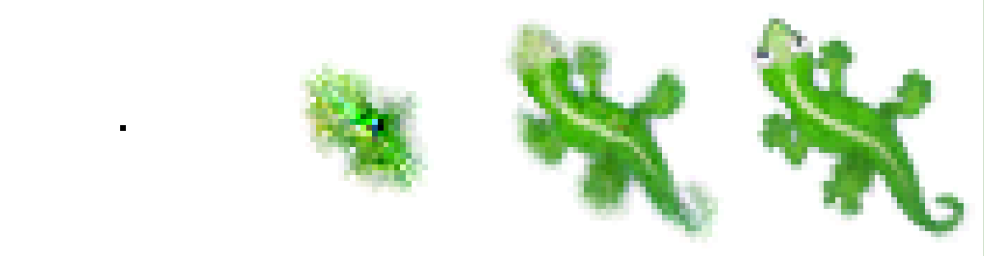
\includegraphics[width=0.6\linewidth]{img/morfogenesis.png}
	\caption{Evolución del \textit{emoji} de una lagartija a partir de una única célula activa después de 219 pasos evolutivos \cite{mordvintsev2020_nca}.}
	\label{fig:morfogénesis}
\end{figure}

El autómata celular neuronal diseñado tiene las siguientes características (las cuales fueron retomadas por múltiples autores que tomaron a \cite{mordvintsev2020_nca} como referencia):

\begin{itemize}
	
	\item El vector de cada célula (cada valor en un rango de $[0,1]$) incluye los canales RGB y un canal $\alpha$ que funciona como umbral para definir si una célula está viva o muerta (establece el resto de valores del vector a $0$ si $\alpha \leq 0.1$). 
	
	Considerando las dimensiones $(\text{largo}, \text{ancho}, 16)$ y un kernel de $3 \times 3$ y se calcula el gradiente en las dos direcciones ($x$ y $y$) usando un filtro Sobel. Esto genera un nuevo vector que se utilizará como entrada para la red neuronal.
	\[ 
	16 (\text{estado propio}) + 16 (\text{gradiente en } x) + 16 (\text{gradiente en } y) = 48 
	\]
	\item Se usaron convoluciones de $1 \times 1$ con una función \textit{ReLU} y alrededor de $8000$ parámetros entrenables y devuelve un $\delta$ que se suma al estado actual de célula antes del siguiente paso. 
	
	
	
	\item Se omite el cálculo para las células muertas y la actualización de cada célula se realiza con una probabilidad del $50\%$. La actualización debe ser estocástica para lograr un mejor rendimiento \cite{niklasson2021_nca}. 
	
\end{itemize}

Eyvind Niklasson et al. \cite{niklasson2021_nca} compararon el rendimiento del modelo en \cite{mordvintsev2020_nca} con actualización síncrona y asíncrona. Donde, tras haber llevado a cabo pruebas con diferentes tamaños de paso, concluyeron que la función de pérdida crece exponencialmente cuando la actualización es síncrona. Sin embargo, esto ocurre únicamente cuando el tamaño de paso es mayor que uno.

Una hipótesis de este comportamiento es que, al tener células que se actualizan en diferentes periodos de tiempo, cada célula puede conocer parte del contexto de su vecindad. Esto no se logra únicamente conociendo los valores actuales de cada vecino.

Se realizaron los siguientes experimentos en \cite{mordvintsev2020_nca}:

\begin{enumerate}
	
	\item Crecer una única célula activa para formar una figura dada mediante \textit{backpropagation}. Cuando el autómata celular llega a la figura deseada, si se siguen aplicando las reglas de evolución, puede crecer sin límites, quedarse en la misma figura, eliminar todas las células o crear patrones que son caóticos o que se repiten.
	
	
	
	\item Convertir las figuras objetivo en atractores usando \textit{sample pool}. Se entrenó mediante múltiples condiciones iniciales, obtenidas a partir de entrenamientos fallidos, para llegar al objetivo desde diferentes configuraciones. 
	
	
	
	\item Regenerar partes de la figura. Se eliminaron partes de la figura objetivo y se añadieron al conjunto de entrenamiento.
	
	
	
	\item Rotaron la figura objetivo. Dado que los filtros de Sobel funcionan como direcciones ortogonales, se puede aplicar una rotación mediante: 
	\[ \begin{bmatrix}
		K_x & K_y
	\end{bmatrix} = \begin{bmatrix}
		cos \theta & -sin \theta \\
		sin \theta & cos \theta
	\end{bmatrix} \cdot \begin{bmatrix}
		Sobel_x & Sobel_y
	\end{bmatrix} \]
	Para modificar el ángulo sin necesidad de reentrenar el modelo.
	
\end{enumerate}

\subsubsection{Autómatas celulares neuronales isotrópicos}

En \cite{mordvintsev2022_iso_nca}, \cite{mordvintsev2022_iso_nca2} y \cite{mordvintsev2023_snca}, Mordvintsev et al. presentan una nueva configuración que no tenga una dirección preferida, la cual nombraron autómatas celulares neuronales isotrópicos.

Para que esta regla sea isotrópica, es necesario que sea independiente de la dirección (sin distinguir ``arriba'' de ``izquierda''). Esto permite crear rotaciones o simetrías sin que el sistema se descontrole.

Se sustituyen las funciones de los filtros de Sobel en \cite{mordvintsev2020_nca} por un único filtro laplaciano:
\[
K_{lap} = \begin{bmatrix}
	1 & 2 & 1 \\
	2 & -12 & 2 \\
	1 & 2 & 1 	
\end{bmatrix}
\]
El cual se concatena al vector de cada célula y alimenta a una red neuronal artificial de $9408$ parámetros. 

A continuación, se describen los resultados obtenidos con dos diferentes enfoques:
\begin{enumerate}
	\item Estrategia de semilla estructurada: Se necesitan al menos tres células con valores diferentes y no colineales para definir la orientación y la posición. Modificar la posición de estos puntos implica una evolución acorde a la posición de los mismos.
	
	\item Estrategia de una única semilla: Se modifica la función de pérdida para que sea invariante ante rotaciones y reflejos. Para evitar comparar la figura resultante con todas las rotaciones posibles, se mapean ambas figuras a coordenadas polares y, para cada posible ángulo de rotación, se calcula la diferencia. Para disminuir la complejidad computacional, se aplica la transformada rápida de Fourier y se hace uso del teorema de la convolución:
	\[
	s * t = \mathcal{F}^{-1} (\mathcal{F}(S) \cdot \mathcal{F}(T)) 
	\]
	Se obtienen todas las diferencias únicamente como una multiplicación de transformadas.
	
	Para evitar que se formen patrones simétricos mezclados (como figuras con cabeza-cabeza o cola-cola), se agrega un nuevo canal llamado \textit{binary auxiliary channel} que da valores de $-0.5$ y $0.5$ a la parte superior e inferior de la imagen, respectivamente.
	
	Con estas nuevas configuraciones se puede obtener el mismo resultado que en \cite{mordvintsev2020_nca}, pero sin la dependencia de una dirección explícita y con una red neuronal artificial con menos parámetros.
	
\end{enumerate}

\subsubsection{Autoclasificación}

En \cite{mordvintsev2020_mnist} Mordvintsev utiliza los autómatas celulares neuronales para la autoclasificación de MNIST\footnote{Conjunto de datos de imágenes $28 \times 28$ de números en el rango $[0,9]$} las cuales fueron binarizadas con un umbral de $0.1$. 

El objetivo es que, a partir de una configuración inicial de células vivas, el sistema pueda reconocer la forma solo usando reglas locales. En este caso, se trata de identificar los números de MNIST.

Estos son los cambios del autómata celular MNIST respecto al modelo original \cite{mordvintsev2020_nca}:

\begin{itemize}
	
	\item Vector de la célula: Originalmente se usaban los canales RGB; ahora se emplean 10 canales que funcionan como distribución de probabilidad de cada posible número. Durante la evaluación se utiliza el mayor de ellos.
	
	\item Célula viva o muerta: En \cite{mordvintsev2020_nca} se define mediante el canal $\alpha$, pero las células muertas siguen siendo visibles para el resto. En \cite{mordvintsev2020_mnist}  únicamente interactúan las células vivas.
	
	\item Topología: Todas las células son un único componente conexo.
\end{itemize}

Con el nuevo modelo, Mordvintsev pudo realizar clasificaciones con una precisión del $95.3\%$ con una función de pérdida $L_2$ y ruido añadido. Este experimento demostró que los autómatas celulares neuronales no solo pueden generar patrones y autorregenerarse, sino también realizar tareas de clasificación distribuidas sin una capa de decisión global.

Aunque los modelos en \cite{mordvintsev2020_nca} y \cite{mordvintsev2020_mnist} son robustos frente a diferentes tipos de perturbaciones, su comportamiento se puede ver afectado por estados individuales de las células, parámetros del modelo y el campo perceptivo (la manera en cómo las células perciben su vecindad).

Es por esto que Randazzo et al. \cite{mordvintsev2021_a_nca} buscan enfrentar estrategias adversarias en el mismo espacio celular para estudiar la reprogramación de los autómatas celulares mediante dos experimentos:
\begin{enumerate}
	\item \textbf{Inyección de adversarios}: Se entrena un nuevo modelo de autómata celular, que se coloca en el entorno que ejecuta uno de los modelos originales, para secuestrar el comportamiento del colectivo.
	
	\item \textbf{Perturbación de estados}: A un modelo ya entrenado, se le aplican perturbaciones a todas las células del sistema de forma simultánea.
\end{enumerate}

Para la inyección de adversarios se utilizan dos modelos: el modelo original del autómata celular para MNIST con probabilidad de $90\%$ y un nuevo modelo que clasifica a todos los números como ``ocho'' ($10\%$).  Se introducen varias células invasoras en figuras que ya han sido clasificadas, y estas células muestran un comportamiento dominante al clasificar todos los elementos como ``ocho''. Además, una vez retiradas las células invasoras, el sistema es capaz de recuperarse la mayoría de las veces.

Sin embargo, al aplicar el mismo procedimiento para \cite{mordvintsev2020_nca}, los resultados no tuvieron el mismo rendimiento. Probaron modificar la morfología de la imagen de una lagartija sin cola y con otro color, pero ninguna estrategia fue capaz de invadir por completo el modelo original. 

Una hipótesis es que para MNIST no necesita cambiar completamente su valor para producir algo diferente de lo que generaba antes, ya que el estado de la mutación es un estado que el modelo original ya tenía en cuenta. Por otro lado, al cambiar el color y la forma en \cite{mordvintsev2020_nca}, se están explorando configuraciones nunca antes vistas por el modelo original.

Para el segundo experimento (perturbación de estados), se sigue la línea de modificar el color y la forma de la imagen de una lagartija. Se aplica una perturbación global de estados cada paso de tiempo con el objetivo de identificar la perturbación específica que dé como resultado un patrón estable.

En cada paso evolutivo, se multiplica el vector de cada célula por una matriz simétrica $A$ de $16 \times 16$ \cite{mordvintsev2020_nca}. Para definir los valores de la matriz, se inicia con una matriz simétrica $I$ y, a diferencia del modelo original, la configuración inicial se establece como la figura objetivo del mismo.

Esta configuración permite crecer un sistema con perturbaciones, alterar su forma y color una vez crecido y modificar el impacto y el número de perturbaciones posibles. Al manejar matrices simétricas, se puede representar como 
\[A = Q \Lambda Q^T\] 
donde: 

\begin{itemize}
	
	\item $\Lambda$ es la matriz diagonal de los valores propios.
	
	\item $Q$ es la matriz unitaria de los vectores propios.
	
\end{itemize} 

Si $\Lambda = I \to A = I$, por lo que no existe perturbación (multiplicación por matriz identidad). Bajo esta premisa, se propone la siguiente fórmula:
\[ A_k = Q(kD + I)Q^T\]
Donde:

\begin{itemize}
	
	\item $A$ es la matriz original.
	
	\item $k$ es el factor de escala.
	
	\item $D$ es la dirección de la perturbación $\Lambda - I$ en el espacio de valores propios. 
	
\end{itemize}

Si $k = 0$, no existe perturbación en el sistema:

\begin{gather*}
	A_k = Q(0D + I)Q^T \\
	A_k = Q I Q^T
\end{gather*}

Si $k = 1$, se conserva la perturbación original:

\begin{gather*}
	A_k = Q(1D + I)Q^T \\
	A_k = Q(\Lambda - I + I)Q^T \\
	A_k = Q \Lambda Q^T
\end{gather*}

Mostrando que se puede escalar el tamaño de la perturbación, incluso con perturbaciones inversas con $k = -1$.

Si consideramos dos perturbaciones cuyos vectores propios son similares: $A_k = Q(k_AD_A + I)Q^T$ y $B_k = Q(k_B D_B + I)Q^T$, podemos combinarlos como
\[ comb(A_k, B_k) = Q (k_A D_A + k_B D_B + I) Q^T = k_A A + k_B B + (1 - k_A - k_B) I \]
Esta nueva combinación permite configurar múltiples perturbaciones, las cuales se vuelven más sensibles conforme aumentan los $k$.

Estos experimentos muestran cómo los autómatas celulares neuronales pueden ser vulnerables a diferentes estrategias y cómo las mutaciones ``exactas'' pueden modificar la estructura de todo el sistema.

Todas estas representaciones han tenido lugar en un espacio bidimensional. A continuación se presentan algunas propuestas en espacios tridimensionales. 

\subsubsection{Representaciones tridimensionales}

Zhang et al. \cite{zhang2021_gca} proponen un modelo generativo tridimensional denominado autómata celular generativo que extiende el paradigma de los autómatas celulares hacia la generación progresiva de formas tridimensionales. A diferencia de enfoques que intentan reconstruir directamente la forma completa, el autómata celular generativo formula el proceso como una cadena de Markov, donde cada paso corresponde a una transición local sobre una rejilla tridimensional. 

El modelo se entrena para que estas reglas locales, al repetirse, converjan hacia formas específicas. Para ello, se representa la forma como puntos de superficie en una rejilla 3D y se emplea una red convolucional dispersa que opera únicamente sobre las regiones activas.

Durante el entrenamiento, se utilizan secuencias ligeramente distintas a las cadenas de muestreo reales, pero que convergen hacia las formas del conjunto de datos. Esto permite que el modelo aprenda reglas de transición robustas, capaces de generar formas diversas desde configuraciones parciales. Con una sola inferencia, el sistema puede tomar diferentes ejemplos de la distribución que ha aprendido, obteniendo buenos resultados en tareas de completar y generar formas en 3D.

Este enfoque es una aportación importante a la morfogénesis computacional, ya que muestra que las reglas locales que se autoorganizan pueden aplicarse a estructuras 3D complejas utilizando redes neuronales adaptadas.

En \cite{zhang2021_gca}, se muestra que la autoorganización local se puede escalar a tres dimensiones. Por otro lado, Shyam Sudhakaran et al. \cite{sudhakaran2021_nca_3d} amplían el trabajo de \cite{mordvintsev2020_nca} a tres dimensiones, usando el juego de Minecraft como espacio celular\footnote{En Minecraft, se pueden crear estructuras estáticas (como árboles) y dinámicas (como máquinas voladoras)}. El autómata celular neuronal entrenado puede crear estructuras de hasta 3584 bloques utilizando 50 bloques diferentes, manteniendo las propiedades de regeneración de su versión en 2D.

Una entidad en Minecraft se representa como una red 3D donde cada elemento es un vector que almacena (1) el tipo de bloque (incrustado en un vector \textit{one-hot}), (2) su estatus (replicando el comportamiento del canal $\alpha$ de \cite{mordvintsev2020_nca}) y (3) estados ocultos.

Se utilizan convoluciones para permitir la generación y manipulación de estructuras 3D. Además, se sustituye el uso de filtros de Sobel por una red de percepción aprendible con un kernel de $3 \times 3 \times 3$, \textit{stride}\footnote{Cuántas posiciones se desplaza el \textit{kernel} sobre la entrada en cada operación de convolución} de 1 y canales de salida equivalentes a tres veces el número de canales del estado celular. Esta red permite que el sistema aprenda activamente a percibir su entorno local, adaptando sus filtros durante el entrenamiento y capturando patrones espaciales relevantes de manera dinámica.

Se utiliza una actualización estocástica y un umbral de activación similar a \cite{mordvintsev2020_nca}. Finalmente, todos los modelos se inicializan con una distribución normal estándar, con media cero y desviación estándar en el rango de $0.0001$ a $0.1$, lo que proporciona un punto de partida estable para el entrenamiento y la evolución del sistema. Este sistema hereda las propiedades regenerativas de su versión 2D.

Finalmente, Horibe et al. \cite{horibe2021_softrobot} llevan las propiedades regenerativas al mundo físico. Se implementa el enfoque regenerativo en robots blandos mediante autómatas celulares neuronales. Cada robot tiene un conjunto de volúmenes de reposo para cada vóxel\footnote{Unidad básica de un espacio tridimensional, similar a un píxel en imágenes 2D, pero con volumen}. Estos volúmenes se activan con una señal global que tiene forma de onda sinusoidal, lo que causa que se expandan y se contraigan. Esta dinámica permite simular locomoción a través de ciclos de actuación, evaluando el desplazamiento del centro de masa como métrica de fitness. Los robots blandos se componen de distintos tipos de vóxeles: músculos en fase y contrafase, huesos rígidos y flexibles, cada uno con un rol en la locomoción.

El modelo entrenado demuestra que los robots blandos pueden recuperar parcialmente su morfología original tras sufrir daño y restaurar su capacidad de movimiento sin intervención externa. Este comportamiento surge de la dinámica autoorganizada del autómata celular neuronal, que codifica de manera implícita la forma objetivo y su capacidad de reparación.

Para evaluar la capacidad de locomoción y regeneración de los robots blandos generados mediante autómatas celulares neuronales, se emplea el simulador físico Voxelyze. Los experimentos se realizan en configuraciones 2D y 3D, utilizando rejillas de $7 \times 7$ y $9 \times 9 \times 9$ vóxeles, respectivamente. Las condiciones de frontera tipo Dirichlet limitan el crecimiento morfológico a regiones internas ($5 \times 5$ en 2D y $7 \times 7 \times 7$ en 3D).

Este entorno permite comprobar cómo los autómatas celulares neuronales se autoorganizan para crear formas que son funcionales y resistentes. Además, proporciona una base cuantitativa para comparar la eficiencia locomotora antes y después de procesos de regeneración. La estructura en vóxeles ayuda a combinar reglas locales y programación distribuida, y se relaciona con modelos inspirados en la biología sobre cómo se forma la estructura.

En conjunto, estos trabajos evidencian cómo los autómatas celulares neuronales pueden extender sus principios regenerativos y de autoorganización a dominios tridimensionales cada vez más complejos. Mientras Autómatas celulares generativos establecen un marco generativo para formas 3D a partir de reglas locales aprendidas, los experimentos en Minecraft muestran que dichas propiedades pueden preservarse incluso en entornos con alta variabilidad estructural. Finalmente, la aplicación en robots blandos confirma el potencial bioinspirado de los autómatas celulares neuronales: no solo permiten generar morfologías funcionales, sino que además dotan a los sistemas físicos de resiliencia ante daños, abriendo camino hacia formas de robótica autorreparable.

Otra forma de implementar los autómatas celulares neuronales en 3D es mediante planos, mallas y texturas autoorganizadas que cubren la superficie de un objeto tridimensional. 

\subsection{Autómata celular neuronal en malla}

Niklasson et al. \cite{mordvintsev2021_mnca} y Mordvintsev et al. \cite{mordvintsev2021_mnca2} \cite{mordvintsev2021_unca} introducen el concepto de texturas autoorganizadas, cuyo objetivo es reproducir la apariencia global de una textura de referencia sin generar copias exactas. Para esto, entrenan un autómata celular neuronal utilizando la misma estructura neuronal que se propuso en \cite{mordvintsev2020_nca}, para que pueda reconocer y crear patrones distintivos como tableros de ajedrez, líneas o mosaicos. Aunque este enfoque tiene un carácter demostrativo, constituye una evidencia significativa de que los autómatas celulares neuronales pueden aprender y generalizar comportamientos visuales locales en lugar de memorizar imágenes específicas.

Niklasson et al. proponen los autómatas celulares neuronales en mallas \cite{mordvintsev2024_mesh_nca}, que es un método creado para crear texturas en movimiento en superficies en 3D. A diferencia de los experimentos en cuadrículas de dos dimensiones, los autómatas celulares neuronales en mallas aplican el mecanismo de autoorganización a mallas de cualquier forma, incluso si están en movimiento. El modelo es consistente en diferentes situaciones, es resistente a cambios externos y permite ajustar características como la densidad, la dirección y la rotación de los patrones que aparecen. Además, varios autómatas celulares neuronales en redes pueden combinarse, creando cambios suaves entre texturas sin interrupciones.

\begin{figure}[!htbp]
	
	\centering
	
	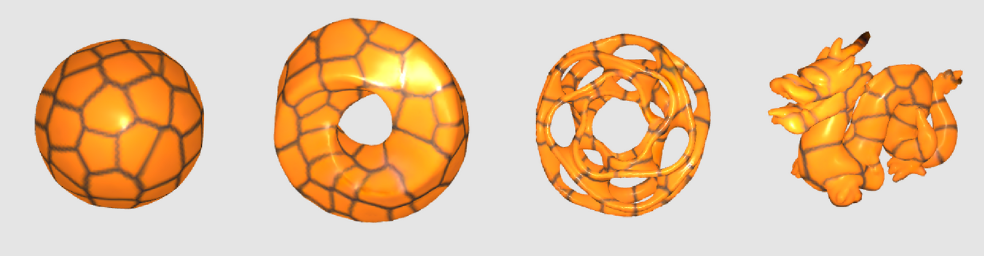
\includegraphics[width=0.75\linewidth]{img/mesh.png}
	
	\caption{El entrenamiento se realiza sobre un poliedro simétrico y el autómata celular neuronal puede ser extrapolado a cualquier objeto tridimensional \cite{mordvintsev2020_nca}.}
	
	\label{fig:mesh}
	
\end{figure}

Sin embargo, este enfoque presenta un reto de escalabilidad. El número de células involucradas suele encontrarse en el rango de $10^4 \sim 10^5$, lo que limita la resolución alcanzable a entre $64 \times 64$ y $256 \times 256$ píxeles. Como el tiempo de entrenamiento escala de forma cuadrática con respecto al número de celdas, el aumento de resolución conlleva un cuello de botella en la propagación de información a lo largo de la malla.

Para solucionar esta limitación, Niklasson et al. sugieren en \cite{mordvintsev2024_mesh_nca2} un modelo híbrido que une autómatas celulares neuronales  con representaciones neuronales implícitas. La idea central es desacoplar el tamaño de la cuadrícula de los autómatas celulares neuronales  de la resolución final, delegando el renderizado detallado a un decodificador ligero denominado red local de producción de patrones. De este modo, el autómata celular neuronal mantiene una cuadrícula explícita y relativamente pequeña que evoluciona de manera local, mientras que la red local de producción de patrones se encarga de producir el color en cualquier punto del espacio continuo a partir de información interpolada de las celdas vecinas.

En términos formales, para cada punto de muestreo $p$, la red local de producción de patrones recibe dos entradas: Una es un estado celular promedio $s(p)$, obtenido mediante interpolación de las celdas cercanas en un primitivo geométrico; la otra es un vector de coordenadas locales $u(p)$, que codifica la posición relativa de $p$ dentro de dicho primitivo. Dependiendo de cómo se divida el espacio, estas formas básicas pueden ser rectángulos, cubos, triángulos o polígonos en general. Estas formas están definidas por coordenadas $\lambda_i(p)$ que deben cumplir con ciertas propiedades, como ser una partición unitaria y no ser negativas. Para asegurar una continuidad en el espacio, se cambian las coordenadas usando funciones sinusoidales en cuadrículas cartesianas o en redes triangulares, creando así campos posicionales suaves.

El resultado es un sistema que conserva las propiedades autoorganizativas de los autómatas celulares neuronales al tiempo que permite alcanzar mayor resolución sin un aumento proporcional del costo computacional. Desde una perspectiva biológica, el autómata celular neuronal puede interpretarse como un plano morfogenético que define la organización global, mientras que la red local de producción de patrones añade los detalles finos sin necesidad de simular interacciones locales a gran escala. Este paralelismo, aunque principalmente ilustrativo, refuerza la idea de que los autómatas celulares neuronales pueden actuar como generadores de estructuras robustas y adaptables, mientras que módulos complementarios aportan precisión y escalabilidad.

A pesar de estas mejoras, una limitación persistente es que cada autómata celular neuronal debe entrenarse de manera específica para una textura o patrón dado. Incluso en escenarios donde múltiples autómatas celulares neuronales coexisten, cada modelo requiere su propio entrenamiento independiente. Esto ha motivado nuevas propuestas orientadas a la construcción de espacios compartidos de autómatas celulares neuronales, capaces de generalizar a múltiples texturas dentro de un mismo marco de entrenamiento.

\subsection{Modelos generativos}

Cada imagen creada con un autómata celular neuronal tiene una red neuronal artificial que ha sido entrenada específicamente para copiar ese comportamiento. Alejandro Hernández et al. \cite{hernandez2021_ncam} proponen unas redes neuronales artificiales de mayor capacidad que permitan crecer múltiples imágenes, a lo que llamaron colector de autómatas celulares neuronales.

El colector de autómatas celulares neuronales usa un modelo de convoluciones dinámicas para modelar un espacio de dichos autómatas. Utiliza un \textit{autoencoder} que se compone de un codificador y un decodificador: El codificador transforma la entrada en una representación continua y luego categórica, que el decodificador reconstruye en el espacio original.

Un elemento destacable de la arquitectura propuesta es un parámetro entrenable llamado \textit{Leak Factor} (LF) que mejora la estabilidad durante el entrenamiento. Este parámetro regula la cantidad de información que se filtra en cada paso del modelo; por ejemplo, un valor bajo retiene el conocimiento acumulado. Este valor se incrementa durante el entrenamiento a medida que mejora el rendimiento.

La arquitectura también emplea convoluciones dinámicas. Los \textit{kernels} se generan a partir del \textit{embedding} de cada instancia, permitiendo adaptabilidad sin modificar la estructura del autómata celular neuronal. El colector de autómatas celulares neuronales inicia desde una imagen semilla y actualiza cada celda mediante percepciones locales (filtros Sobel $+$ normalización) y capas densas por píxel, moduladas por el LF. Se exploran actualizaciones estocásticas y sincrónicas, siendo esta última más precisa y estable, tal como en \cite{niklasson2021_nca}.

Los experimentos muestran que la codificación y la actualización simultáneamente mejoran la calidad de la reconstrucción, incluso sin mecanismos de enmascaramiento. También se observa que aumentar la dimensionalidad del \textit{embedding} mejora significativamente los resultados.

Por otro lado, Kevin Frans en \cite{frans2021_stampca} propone un modelo llamado autómatas celulares neuronales condicionales, cuya semilla recibe un \textit{embedding}, el cual define la imagen en la cual va a crecer. 

Dado un diseño deseado, una red de codificador lo comprime en un \textit{embedding}, el cual se utiliza como condición inicial en el autómata celular neuronal, que luego itera para crecer en la figura objetivo; esto permite crear nuevas configuraciones.

Utilizando un \textit{dataset} con aproximadamente 3000 \textit{emojis} de $32 \times 32$ píxeles, fue capaz de entrenar a un autómata celular neuronal condicional utilizando el mismo método de \cite{mordvintsev2020_nca} para poder dibujar todos los \textit{emojis} con un único autómata celular neuronal.

Para generar números de MNIST, se adopta un enfoque tipo red adversarial generativa, donde el objetivo es crecer dígitos desde ruido aleatorio. Dado que entrenar directamente un autómata celular neuronal como generador de red adversarial generativa resultó inestable, se utilizó una estrategia en dos etapas: (1) Se entrena primero un generador tradicional (\textit{feedforward}) para mapear vectores aleatorios a dígitos MNIST y (2) el autómata celular neuronal se entrena para imitar la salida de ese generador, logrando una generación más estable.

Este enfoque permite que el autómata celular neuronal genere dígitos sin necesidad de un \textit{dataset} explícito, aprendiendo directamente a partir del objetivo de la red adversarial generativa. Además, se observa un patrón de crecimiento distintivo: mientras los \textit{emojis} crecen en ondas desde el centro, los dígitos MNIST se desarrollan siguiendo la forma del trazo.

Mingxiang Chen et al. \cite{chen2020_vaenca} combinan los principios de codificador automático variacional con autómata celular neuronal. Utilizan un \textit{encoder} que transforma una imagen en una distribución de probabilidad, las cuales forman un \textit{embedding}, el cual funciona como condición inicial del autómata celular neuronal. Después, Rasmus Berg Palm et al. \cite{rasmus2022_vnca} llaman a este modelo ``autómatas celulares neuronales variacionales''. También afirman que ninguno de los otros modelos mencionados (\cite{mordvintsev2020_nca}, \cite{hernandez2021_ncam}, \cite{zhang2021_gca}, \cite{horibe2021_softrobot} y \cite{frans2021_stampca}) es realmente generativo.

El autómata celular neuronal variacional aprende una distribución de probabilidad que codifica los datos observados. A partir de esta representación, el \textit{encoder} genera imágenes mediante un autómata celular neuronal que simula el crecimiento espacial desde una semilla. A diferencia del codificador automático variacional, que decodifica la imagen directamente, el autómata celular neuronal variacional utiliza el \textit{embedding} como configuración inicial de una cuadrícula de celdas que evolucionan siguiendo las reglas definidas por una red neuronal convolucional. 

Por otra parte, este modelo incorpora mecanismos de duplicación celular inspirados en la mitosis. Cada $M$ pasos, las celdas se duplican hacia la derecha y hacia abajo, permitiendo a la imagen crecer de manera autoorganizada. 

Los experimentos realizados en \cite{rasmus2022_vnca} demuestran que el autómata celular neuronal variacional es capaz de aprender procesos generativos autoorganizados tanto en dominios simples como MNIST, como en conjuntos más complejos como CelebA\footnote{\textit{Dataset} de imágenes de celebridades}. En MNIST, el modelo logra reconstrucciones precisas y muestras plausibles desde el espacio latente, con una log-verosimilitud de $\log p(x) \geq -84.23$ nats\footnote{Unidad de medida utilizada en aprendizaje automático y estadística para expresar la $\log$-verosimilitud o la entropía de un modelo}; su rendimiento es comparable a modelos autorregresivos como PixelCNN. Además, el análisis del espacio latente muestra una estructura más clara y organizada en comparación con los decodificadores convolucionales tradicionales. Esto indica que la codificación es más semántica y eficiente.

En CelebA, aunque las muestras generadas directamente no alcanzan calidad visual comparable a modelos de última generación, el autómata celular neuronal variacional muestra capacidad de reconstrucción robusta y mejora visual significativa al ajustar el parámetro $\beta$, que regula el equilibrio entre fidelidad de reconstrucción y calidad de generación. 

Finalmente, se explora la resiliencia de los autómatas celulares neuronales variacionales ante daño estructural durante el crecimiento. Al eliminar las capas de duplicación y entrenar con un esquema de recuperación de daño, el modelo aprende dinámicas estables capaces de restaurar imágenes deterioradas casi por completo, incluso tras múltiples pasos de evolución. Este comportamiento sugiere que el autómata celular neuronal variacional no solo codifica la imagen, sino que también es un proceso de reconstrucción en el estado celular.

\subsection{Representaciones y aplicaciones adicionales}

Hasta ahora, muchos de los estudios sobre autómatas celulares neuronales se han enfocado en la morfogénesis, que es el proceso de formación de formas, y en su habilidad para crear estructuras visuales que se organizan solas. Sin embargo, también han surgido enfoques que amplían el marco conceptual hacia nuevas formas de representación y aplicaciones en dominios específicos. A continuación, se presentan algunas de estas variantes.

Mattie Tesfaldet et al. \cite{Tesfaldet2022_vitca} extienden los autómatas celulares neuronales mediante mecanismos de atención inspirados en arquitecturas de \textit{transformers}, dando lugar a autómatas celulares con \textit{transformers} de visión. Esta arquitectura híbrida permite que las interacciones locales tengan acceso contextual a regiones más amplias a través de \textit{self-attention}, lo que habilita organización global sin incurrir en la complejidad cuadrática típica de la atención completa. Los autómatas celulares con \textit{transformers} de visión adaptan el proceso de los \textit{transformers} de visión tradicionales, que dividen una imagen en parches y los convierten en secuencias de \textit{tokens}, al formato de una cuadrícula de celdas, donde cada celda almacena información visual, posicional y oculta. En lugar de aplicar atención global, restringe el cálculo a vecindarios locales, manteniendo así la naturaleza distribuida del sistema y reduciendo el costo computacional. El entrenamiento se realiza de forma iterativa, alternando entre inyectar entradas corruptas y actualizar parcialmente los estados celulares hasta reconstruir la imagen. De este modo, los autómatas celulares con \textit{transformers} de visión combinan eficiencia, capacidad de autoorganización y organización espacial coherente.

En un ámbito distinto, Jian Tang et al. \cite{Jian2023_nca} emplean una red neuronal convolucional para simular el desarrollo de microestructuras en la solidificación de metales. Cada celda del dominio contiene un estado de fase $P\in[0,1]$ (donde $p=0$ representa líquido y $p=1$ sólido), tres ángulos de Euler $\theta=(\alpha_1,\alpha_2,\alpha_3)$ que definen su orientación cristalográfica y la magnitud de subenfriamiento $\Delta T=T_{melting}-T$. La evolución se modela con un autómata celular neuronal que aplica recurrentemente una red neuronal convolucional para predecir los incrementos en fase, orientación y estados ocultos. Estos canales ocultos facilitan el aprendizaje de patrones temporales complejos sin necesidad de reglas explícitas. Con ello, el modelo reproduce fenómenos como crecimiento competitivo o direcciones preferentes, con una eficiencia computacional sustancialmente mayor que la de muchos autómatas celulares tradicionales y con capacidad de generalización fuera del rango de entrenamiento.

Por otro lado, Gordon H. Y. Li et al. \cite{li2024_pnca} proponen el modelo de autómatas celulares neuronales fotónicos, que aprovecha la velocidad y la interconexión masiva de la fotónica para implementar autómata celular neuronal en hardware óptico. A diferencia de arquitecturas convencionales basadas en perceptrón multicapa o red neuronal convolucional, difíciles de trasladar a entornos fotónicos por sus conexiones densas, el autómata celular neuronal fotónico utiliza reglas locales aprendidas mediante técnicas de aprendizaje profundo. Esto permite realizar clasificación de imágenes en sistemas ópticos, donde la actualización celular se implementa mediante interferencia lineal de luz y activaciones ópticas no lineales. Los autores demuestran clasificación binaria con alta precisión utilizando un número muy reducido de parámetros fotónicos programables, mostrando además robustez frente a datos fuera de distribución. El autómata celular neuronal fotónico representa una vía prometedora para llevar el aprendizaje autoorganizado a plataformas fotónicas escalables.

En el ámbito de la biología computacional, Caitlin Grasso y Josh Bongard \cite{grasso2022_enca} introducen los autómatas celulares neuronales potenciados. Esta es una extensión que incorpora el concepto de \textit{empowerment}, la cantidad de control que una célula puede ejercer sobre su entorno, formalizado mediante medidas de información mutua entre acciones pasadas y estados sensoriales futuros. Incluir \textit{empowerment} como un objetivo adicional en las tareas de morfogénesis mejora la capacidad de evolución y genera patrones de crecimiento más fuertes y adaptables. Esto permite que cada célula actúe como un agente independiente dentro de un sistema distribuido y facilita el estudio de la coordinación y comunicación celular desde una perspectiva computacional.

Finalmente, mientras que modelos como autómatas celulares con \textit{transformers} de visión, autómata celular neuronal fotónico o autómatas celulares neuronales potenciados amplían las capacidades arquitectónicas y las plataformas de aplicación de los autómatas celulares neuronales, Richardson et al. \cite{richardson2024_nca} utilizan los autómatas celulares neuronales como herramienta para modelar fenómenos dinámicos complejos. Entrenando autómata celular neuronal mediante optimización basada en gradientes para reproducir trayectorias espacio-temporales generadas por ecuaciones diferenciales parciales (por ejemplo, Gray–Scott), este enfoque captura tanto estructuras transitorias como patrones estacionarios, incluyendo la formación de patrones tipo Turing, y aborda el problema inverso de inferir reglas locales a partir de comportamiento emergente. Con una complejidad de red mínima, los autores muestran capacidad de generalización, respeto por simetrías y robustez frente a perturbaciones, posicionando a los autómatas celulares neuronales como un marco explicativo y eficiente para sistemas biológicos y físicos.

Se observa que los autómatas celulares neuronales han evolucionado desde sus primeras aplicaciones en morfogénesis, donde se exploró su capacidad de generar estructuras complejas partiendo de una única célula activa, hacia modelos que buscan una mayor versatilidad generativa, capaces de producir dinámicas visuales, texturas, comportamientos adaptativos e incluso manipular estrategias, muchos de ellos inspirados en la definición de Mordvintsev. Además, se han desarrollado arquitecturas híbridas que no generan un autómata celular neuronal individual, sino que modelan un espacio de autómatas semejantes, así como configuraciones generativas y bioinspiradas.

En resumen, estos estudios muestran que los autómatas celulares neuronales no solo son un concepto interesante desde el punto de vista teórico, sino que también son útiles en inteligencia artificial, ciencias naturales e ingeniería. Esta diversidad de enfoques abre la puerta a explorar nuevas adaptaciones y propuestas, especialmente en áreas de aprendizaje profundo, autoorganización y simulación de procesos dinámicos.	

	\chapter{Marco metodológico}

El marco metodológico se constituye como el resultado de la aplicación sistemática y lógica de los conceptos y fundamentos abordados en el marco teórico. Azuero et al. \cite{azuero2019_metodologico} lo definen como un conjunto de acciones destinadas a describir y analizar el fondo del problema planteado, mediante procedimientos específicos que incluyen técnicas de observación y recolección de datos, los cuales determinarán el cómo se llevará a cabo la investigación. 

Este capítulo se dividirá en secciones que definan la estructura del marco metodológico, con el fin de sustentar los métodos y recursos elegidos para el desarrollo de la investigación. Se asegurará que cada fase esté alineada con los principios teóricos fundamentales y que los resultados obtenidos sean fiables, replicables y efectivos en el tratamiento de la problemática planteada.

\section{Diseño de la investigación}

El diseño de la investigación establece la estrategia general con la que se responde a la pregunta de investigación. En este trabajo se adopta un diseño experimental, cuya variante cuasiexperimental se detalla a continuación.

\subsection{Diseño experimental}

El diseño experimental es un método sistemático para planificar, ejecutar y analizar experimentos, con el objetivo de identificar relaciones causales entre variables. En otras palabras, se manipula una variable independiente para observar su efecto sobre la variable dependiente \cite{unam2025_experimental}.

De acuerdo con su nivel de control, los diseños experimentales se clasifican en tres tipos: preexperimentos, cuasiexperimentos y experimentos puros. En el presente trabajo se adopta un diseño cuasiexperimental por las características propias del entorno de simulación y la naturaleza del objeto de estudio.

El diseño experimental resulta apropiado en este contexto. Se manipula una variable independiente (la definición de la función de transición mediante una red neuronal) para observar sus efectos sobre el comportamiento del sistema simulado. Esto se hace sin que exista una asignación aleatoria ni un grupo de control en un sentido estricto. 

\subsubsection{Diseño cuasiexperimental}

El diseño cuasiexperimental busca establecer relaciones causales sin la necesidad de asignar aleatoriamente a los participantes o unidades experimentales a los grupos de estudio. Se caracteriza por la existencia de una intervención deliberada sobre una variable independiente, mientras que los grupos de comparación se definen con base en condiciones preexistentes \cite{capili2024_cuasiexperimento}.

En el caso de esta investigación, el estudio se desarrolla en un entorno computacional controlado, donde las condiciones experimentales se reproducen mediante simulaciones. El objetivo principal es estudiar cómo diferentes factores, como la forma de la red neuronal o la configuración del autómata, afectan los patrones que aparecen en los autómatas celulares neuronales. Este enfoque permite observar efectos y comportamientos resultantes, manteniendo un control suficiente sobre las variables involucradas sin requerir un esquema de aleatorización.

\section{Enfoque de la investigación}

Este proyecto utiliza un enfoque cuantitativo, que se basa en recoger y analizar datos numéricos para describir fenómenos a través de métodos estadísticos y matemáticos \cite{jaen_cuantitativa}. Este enfoque prioriza la objetividad y medición precisa para establecer relaciones causales entre las variables observadas.

A diferencia de los enfoques cualitativos o mixtos, este no requiere de estudiar percepciones, significados ni experiencias humanas, por lo que es adecuado para investigaciones donde las variables pueden ser definidas, controladas y medidas \cite{cueva2023_mixto}.

El enfoque cuantitativo se justifica porque el análisis se realiza a partir de datos generados mediante simulación computacional. En este proceso no hay intervención directa con humanos y los resultados obtenidos no están sujetos a interpretaciones. Este enfoque permite comparar escenarios, desempeño de modelos e influencia de parámetros sobre la dinámica emergente del sistema.

\section{Población}

La población de estudio se define como un conjunto cerrado, finito y accesible de casos (personas, animales, expedientes, objetos, etc.), los cuales cumplen con un criterio de inclusión y que sirven como base para la investigación \cite{arias2016_poblacion}. En otras palabras, es un conjunto conformado por todos los elementos a los que se pretende generalizar los resultados del estudio.

En este trabajo, la población que se estudia está formada por todos los autómatas celulares finitos que se encuentran en un espacio bidimensional con una distribución de cuadrícula regular. Se consideran condiciones de frontera, un conjunto de estados finito y cualquier función que pueda mapear de $\mathbb{R}^{|\mathcal{N}|} \to \mathbb{R}$.

\section{Muestra y muestreo}

La muestra corresponde a un subconjunto de la población de estudio y consiste en el número de casos que realmente serán estudiados. Esta debe ser representativa para garantizar la validez de los resultados. Por otro lado, el muestreo se refiere al proceso aplicado por el investigador para seleccionar a los participantes dentro de la población \cite{diaz2017_muestra}.

Existe el muestreo probabilístico, donde cada miembro de la población tiene una probabilidad de ser escogido; y el no probabilístico, donde la selección se basa en la conveniencia, el juicio del investigador u otros criterios \cite{diaz2017_muestra}. 

Para esta investigación se realiza un muestreo no probabilístico intencional, donde los elementos seleccionados para la muestra son elegidos por el criterio del investigador. Esto se justifica, ya que, al existir una infinitud de autómatas celulares dadas las restricciones en la población, es necesario delimitar y tratar de replicar los comportamientos. Además, dado que cada autómata celular resuelve un problema, es necesario identificar de forma precisa el problema que se está resolviendo \cite{elsevier2016_computational_biology}.

\section{Tipo de investigación}

Con base en los objetivos, esta investigación se considera aplicada. La investigación aplicada, también conocida como práctica o empírica, se caracteriza porque busca poner en práctica o utilizar los conocimientos adquiridos. En este tipo, las consecuencias prácticas son un interés primordial del investigador \cite{veracruz_aplicada}.

Además, se utiliza un diseño cuasiexperimental, porque se cambian variables independientes para ver cómo afectan los resultados de la simulación, sin tener un grupo de control o asignar condiciones experimentales de forma aleatoria. 

Este tipo de investigación es útil porque ayuda a encontrar relaciones de causa y efecto entre los elementos del modelo y los comportamientos que surgen en el sistema, mientras se mantiene un entorno computacional que es controlado y se puede repetir.

\section{Técnicas e instrumentos de recolección de datos}

La recolección de datos se realiza a partir de las simulaciones computacionales ejecutadas. Dado que se trata de un enfoque cuantitativo, no es necesario usar técnicas como la observación o las encuestas, sino procedimientos de registro automatizado para su posterior análisis numérico. 

\subsection{Técnicas de recolección de datos}

\begin{itemize}
	
	\item Simulación computacional: Ejecución del modelo del autómata celular bajo diferentes configuraciones de vecindad, estados y arquitectura de la red neuronal artificial.
	
	\item Registro automático de datos: Datos generados por la simulación, como el historial evolutivo, patrones y métricas de estabilidad, error y desempeño.
	
	\item Análisis estadístico: Se aplican métricas cuantitativas que permiten comparar configuraciones para evaluar la efectividad del modelo, como la exactitud, la convergencia, la tasa de error y el comportamiento temporal de los patrones.
	
\end{itemize}

\subsection{Instrumentos de recolección de datos}

Se consideran los siguientes instrumentos para obtener y analizar los datos:

\begin{itemize}
	
	\item Simulador desarrollado: Herramienta computacional implementada en C++/CUDA, con una interfaz en Python, que permite ejecutar y visualizar el comportamiento de los autómatas celulares neuronales.
	
	\item Códigos de registro y procesamiento: Conjunto de programas auxiliares que capturan las métricas numéricas de cada simulación y las almacenan en archivos.
	
	\item Herramientas de análisis estadístico y visualización: Bibliotecas y herramientas que permiten obtener representaciones gráficas con los datos obtenidos. 
	
\end{itemize}

\section{Procedimiento}

El desarrollo metodológico de la investigación se llevará a cabo en diversas fases secuenciales. Estas abarcan desde el diseño e implementación del simulador hasta la evaluación del modelo de autómatas celulares neuronales. Cada fase está orientada a cumplir los objetivos planteados y a generar datos cuantitativos que permitan analizar el comportamiento de los sistemas simulados.

\begin{itemize}
	
	\item \textbf{Diseño, desarrollo e implementación del simulador}: Se construye una herramienta computacional capaz de simular autómatas celulares bidimensionales. Aunque el fin último es estudiar los autómatas celulares neuronales, este simulador debe poder aceptar configuraciones clásicas. Esto se debe a que, para las siguientes fases, es necesario conocer el comportamiento de configuraciones conocidas.
	
	\item \textbf{Diseño, desarrollo e integración del módulo de red neuronal artificial}: Se implementa un módulo adicional que permite entrenar una red neuronal artificial para aprender el comportamiento de autómatas celulares existentes. La salida de este módulo es la función de transición aprendida. Además, este módulo se integra dentro del simulador principal para permitir la experimentación directa.
	
	\item \textbf{Imitación de patrones conocidos}: Se diseñan y ejecutan experimentos para evaluar la capacidad del modelo neuronal de imitar el comportamiento de autómatas celulares clásicos, como el juego de la vida. Se busca, además, medir la exactitud del aprendizaje y la estabilidad de las configuraciones generadas. 
	
	\item \textbf{Simulación de otros sistemas complejos}: Una vez validado el funcionamiento del modelo neuronal, se aplican las mismas técnicas a simulaciones que representen otros sistemas complejos. Se busca probar diferentes configuraciones iniciales y parámetros para analizar la capacidad de generalizar la aparición de nuevos patrones.
	
\end{itemize}

Cada una de estas etapas genera resultados que ayudan a mejorar el proceso de desarrollo. Esto permite ajustar tanto la estructura de la red neuronal como las condiciones del simulador.

\section{Técnicas y herramientas de procesamiento de datos}

Una vez recolectados los datos provenientes de las simulaciones computacionales, es fundamental aplicar técnicas adecuadas de procesamiento y análisis para garantizar la validez de los resultados y su correcta interpretación. Dado que el enfoque de la investigación es cuantitativo, el procesamiento se centra en el análisis numérico de los datos generados por el simulador, permitiendo identificar patrones, tendencias y relaciones entre las variables del sistema.

\subsection{Procesamiento de datos cuantitativos}

Los datos cuantitativos se obtienen de las ejecuciones del simulador, donde se registran variables como número de pasos, estados promedio de las células, métricas de error y estabilidad de los patrones emergentes durante un periodo determinado. Posteriormente, estos datos se organizan, procesan y analizan mediante herramientas estadísticas y de visualización.

\begin{itemize}
	\item \textbf{Análisis estadístico descriptivo}: Se calculan medidas de tendencia central y de dispersión con el fin de describir cuantitativamente el comportamiento de las variables analizadas y detectar posibles irregularidades o tendencias \cite{question2023_estadistico}.
	
	\item \textbf{Visualización de datos}: Se elaboran gráficos de barras, histogramas y diagramas de dispersión para representar visualmente los resultados obtenidos, facilitando la comprensión de la dinámica del sistema y la comparación entre diferentes configuraciones experimentales.
\end{itemize}

El procesamiento y análisis de los datos se lleva a cabo utilizando herramientas computacionales. Los resultados obtenidos servirán como base para la interpretación y discusión en las etapas posteriores de la investigación.

\section{Contextualización de la tecnología}

El desarrollo de un simulador de sistemas complejos mediante autómatas celulares neuronales implica la integración de múltiples tecnologías, seleccionadas estratégicamente para satisfacer los requerimientos funcionales y técnicos del proyecto. Esto incluye crear una interfaz gráfica de usuario fácil de usar, simular autómatas celulares en dos dimensiones con diferentes estados, vecindades y reglas de transición, personalizar las condiciones iniciales y entrenar sistemas para que imiten comportamientos que el usuario proporciona.

La elección de estas tecnologías responde a criterios de compatibilidad, escalabilidad, facilidad de implementación y disposición de herramientas específicas para el procesamiento de datos e inteligencia artificial. 

Con el fin de proporcionar una visión clara y completa de las bases técnicas del proyecto, a continuación se presentan el área de estudio (elementos clave para orientar el desarrollo del simulador y validarlo), los fundamentos y el contexto de las tecnologías utilizadas, y los entornos de trabajo que hacen posible este proyecto. 

\subsection{Fundamentos y contexto de las tecnologías}

Un lenguaje de programación es una herramienta que permite el desarrollo de \textit{software} y programas para computadora. Se emplea para diseñar programas encargados de definir el comportamiento físico y lógico de una computadora \cite{uapa2025_lenguajes}.

Debido a que la elección del entorno y lenguaje de programación resulta crítica para el éxito de cualquier proyecto, es importante considerar las metas y alcances del mismo, puesto que no todos los lenguajes son óptimos para resolver ciertos tipos de problemas \cite{clickpanda2023_entorno}.

Entre los factores clave para la elección de un lenguaje de programación se encuentran la escalabilidad, el rendimiento, el costo de mantenimiento, la compatibilidad y el sistema de herramientas, entre otros \cite{clickpanda2023_entorno}.

Es por esto que, como lenguajes de programación, se decidió utilizar C++/CUDA para el núcleo de simulación y cálculos pesados en paralelo, y Python para la interfaz, visualización, control de simulación y diseño de redes neuronales. 

A continuación se presentan las definiciones pertinentes de los lenguajes de programación, \textit{frameworks} y bibliotecas utilizadas para el desarrollo del simulador.

\subsubsection{C++}

C++ es un lenguaje de programación compilado y multiparadigma desarrollado como una extensión de C \cite{valladolid_c}. Se considera un lenguaje de nivel medio, ya que permite manipular directamente la memoria, lo que lo convierte en un lenguaje versátil. Es orientado a objetos, permite la creación de clases y objetos y es ampliamente utilizado para aplicaciones que requieren un alto rendimiento.

Es utilizado en motores de videojuegos, \textit{software} de sistemas, aplicaciones en tiempo real, simulaciones científicas y cálculo numérico \cite{msmk2025_c}. Para esta investigación, se utilizarán las siguientes bibliotecas de C++:

\begin{itemize}
	\item \textbf{iostream}: Declara objetos que controlan la lectura y escritura de datos de un programa en C++ \cite{microsoft2025_iostream}.
	
	\item \textbf{algorithm}: Contiene funciones que realizan algoritmos comunes \cite{microsoft2025_algorithm}.
	
	\item \textbf{cstring}: Funciones que permiten la manipulación de memoria \cite{microsoft2024_cstring}.
\end{itemize}

\subsubsection{CUDA}

CUDA es una plataforma de computación paralela y un modelo de programación desarrollado por NVIDIA que permite utilizar la GPU para cálculos de propósito general. Se emplea para acelerar operaciones matemáticas y simulaciones que requieren grandes cantidades de procesamiento paralelo \cite{cuda}, como el entrenamiento de redes neuronales o la simulación de autómatas celulares.

Se requiere de la biblioteca \textbf{cuda\_runtime}, la cual le permite a un programa escrito en C/C++ usar los núcleos CUDA de una tarjeta gráfica de NVIDIA \cite{cuda_runtime}. Esto permite gestionar la memoria, controlar los núcleos, manejar errores y dispositivos.

\subsubsection{Python}

De acuerdo con la página oficial de la documentación de Python \cite{pythonTutorial}, es un lenguaje de programación potente y fácil de aprender. Tiene estructuras de datos de alto nivel, sintaxis elemental y elegante, un tipado dinámico, naturaleza interpretada, etc. 

Además de ser gratuito, se puede integrar bien en todos los equipos y sistemas. En adición a esto, \cite{awsPython} señala que entre los beneficios que Python incluye se encuentran los siguientes:

\begin{itemize}
	\item Los programas son fáciles de leer y comprender.
	
	\item Mayor productividad al escribir un programa con menos líneas de código en comparación con muchos otros lenguajes de programación.
	
	\item Se puede usar fácilmente con otros lenguajes de programación.
	
	\item Soporte rápido de la comunidad.
	
	\item Se puede trasladar a través de diferentes sistemas operativos de computadora.
\end{itemize}

En adición a lo anterior, cuenta con una amplia colección de bibliotecas y \textit{frameworks} diseñados para tareas que resultaron muy convenientes en el desarrollo de simuladores. A continuación se detallan tanto las bibliotecas como los \textit{frameworks} a utilizar.

\begin{itemize}
	\item\textbf{NumPy} es una biblioteca de Python especializada en el cálculo numérico y el análisis de datos. Es ideal para el manejo de grandes volúmenes de datos \cite{alfaro_numpy}.
	
	Puede hacer operaciones hasta 50 veces más rápido que las listas normales usando un objeto llamado arreglo que permite representar colecciones de datos en varias dimensiones \cite{alfaro_numpy}.
	
	\item\textbf{PyTorch} es una biblioteca de tensores optimizada para el aprendizaje profundo utilizando GPU y CPU \cite{pytorch_1}. Se emplea para crear redes neuronales, combinando la biblioteca de aprendizaje automático de Torch con una API (\textit{Application Programming Interface}, interfaz de programación de aplicaciones) de alto nivel basada en Python. 
	
	Es uno de los marcos de aprendizaje automático destinados a comunidades académicas y de investigación por su flexibilidad y sencillez de uso, además de admitir una amplia variedad de estructuras de redes neuronales \cite{pytorch_2}.
	
	\item \textbf{PyQt5 / PySide6} son herramientas que permiten usar Python como un lenguaje alternativo de desarrollo de aplicaciones a C++ en todas las plataformas soportadas \cite{qt_1}. PyQt5 también puede integrarse en aplicaciones basadas en C++ para permitir a los usuarios de dicho \textit{software} configurar o mejorar la funcionalidad de las mismas, mientras que PySide6 ofrece compatibilidad oficial con las bibliotecas Qt desarrolladas por The Qt Company \cite{qt_2}.
	
	\item \textbf{pybind11} es una biblioteca de C++ diseñada para exponer tipos y funciones de C++ en Python y viceversa, facilitando la creación de extensiones de Python basadas en código C++ \cite{pybind_pybind}. Puede generar enlaces entre ambos lenguajes de manera compacta, eficiente y con un código más simple, posibilitando así integrar cálculos de alto rendimiento escritos en C++ dentro de entornos Python.
	
	\item\textbf{Matplotlib} es una biblioteca de Python especializada en la creación de gráficos en dos dimensiones \cite{alferez_matplotlib}.
	
	Además, mencionan que permite crear y personalizar los gráficos más comunes, entre los que se encuentran:
	\begin{itemize}
		\item Diagramas de barras.
		\item Histogramas.
		\item Diagramas de sectores.
		\item Diagramas de caja y bigotes.
	\end{itemize}
	
	\item \textbf{Scikit-learn} es una biblioteca que cuenta con algoritmos de clasificación, regresión, \textit{clustering} y reducción de dimensionalidad, etc. Es compatible con otras bibliotecas de Python \cite{mds_scikitlearn}.
\end{itemize}

\subsubsection{Wolfram Mathematica}

Es un sistema de computación científica que sigue el paradigma de programación simbólica. Fue desarrollado por Wolfram Research y se especializa en manejar matemáticas complejas, algoritmos de visualización y manipulación de datos de forma nativa \cite{mathematica_2024}. Algunas de sus funcionalidades son:
\begin{itemize}
	\item Visualización: Genera gráficos en 2D y 3D, mapas y diagramas dinámicos.
	
	\item Procesamiento de datos: Herramientas para aprendizaje automático, procesamiento de imágenes y señales.
	
	\item Documentos interactivos: Se trabaja en cuadernos, los cuales mezclan código ejecutable, texto enriquecido, imágenes y modelos interactivos.
\end{itemize}

Adicionalmente, en Wolfram Mathematica existen funciones nativas para construir, evolucionar, manipular y analizar autómatas celulares, por lo que su uso como medio de referencia en la construcción del simulador y como herramienta de análisis de datos resulta fundamental (Wolfram Mathematica no tiene interacción directa con el simulador, únicamente se usa para el estudio de los resultados obtenidos mediante el simulador).

\subsection{Entornos de trabajo}

El desarrollo del presente proyecto requiere de un entorno flexible y bien estructurado que facilite tanto la construcción como la validación de los distintos componentes del sistema. Para ello, se han seleccionado diversas plataformas que permiten organizar tareas, escribir y probar código, almacenar datos, así como documentar y presentar avances.

\subsubsection{Plataformas de desarrollo}

Con el fin de cubrir las distintas etapas del proyecto, desde la implementación hasta la comunicación de resultados, las siguientes plataformas han sido clave para mantener un flujo de trabajo continuo y bien coordinado.

\begin{itemize}	
	
	\item\textbf{Visual Studio Code} es un editor de código gratuito, de código abierto y compatible con múltiples sistemas operativos. Fue creado por Microsoft, empresa con amplia trayectoria en el desarrollo de entornos integrados (IDE), lo que se refleja en la eficiencia y funcionalidad que ofrece esta herramienta, muy valorada por la comunidad de desarrolladores \cite{cimas2024vscode}.
	
	Aunque su nombre puede sugerir una relación directa con Visual Studio, en realidad Visual Studio Code es una aplicación independiente, construida desde cero con tecnologías diferentes. Mientras Visual Studio se orienta principalmente a tecnologías propias de Microsoft, VSCode destaca por su flexibilidad y capacidad de adaptarse a prácticamente cualquier lenguaje de programación \cite{garcia2024vscode}.
	
	\item\textbf{GitHub} es una plataforma basada en la nube donde se puede almacenar, compartir, versionar y escribir código junto con otros usuarios \cite{github2025about}. En adición a lo anterior, también permite realizar lo siguiente:
	
	\begin{itemize}
		\item Presentar o compartir el trabajo.
		\item Seguir y administrar los cambios en el código a lo largo del tiempo.
		\item Dejar que otros usuarios revisen el código y realicen sugerencias para mejorarlo.
		\item Colaborar en un proyecto compartido, sin preocuparse de que los cambios afecten al trabajo de los colaboradores antes de que esté listo para integrarlos.
	\end{itemize}
	
	El versionamiento, una de las características fundamentales de GitHub, es posible gracias al \textit{software} de código abierto Git, en el que se basa GitHub \cite{github2025about}.
	
	\item\textbf{Canva} es una herramienta de diseño y publicación \textit{online}, lanzada en 2013, que tiene como misión poner el poder del diseño al alcance de todo el mundo, para que cualquier persona pueda crear lo que quiera y publicarlo donde quiera \cite{canva2025about}.
	
	\item\textbf{TeXstudio} es un entorno de escritura integrado para la creación de documentos LaTeX. Cuenta con numerosas características como resaltado de sintaxis, visor integrado, comprobación de referencias y varios asistentes. TeXstudio es de código abierto y está disponible para todos los principales sistemas operativos \cite{texstudio}.
	
	\item \textbf{draw.io} es una herramienta de \textit{software} gratuita diseñada para la creación de diagramas. Se utiliza para modelado UML, documentación de proyectos y gestión de flujos \cite{drawio2024}.
	
\end{itemize}

Habiendo definido el enfoque metodológico, justificado las decisiones técnicas del estudio y contextualizado la tecnología utilizada, se cuenta con una base sólida para la implementación y ejecución de los experimentos. Esto permite garantizar que las simulaciones se realicen bajo condiciones controladas, que los datos recolectados sean confiables y que los análisis posteriores aporten resultados válidos y pertinentes para responder a las preguntas de investigación planteadas.


	\chapter{Análisis de software}

Hasta el momento conocemos la metodología utilizada para la investigación completa; sin embargo, es necesario especificar el desarrollo del software, ya que es necesario garantizar el correcto diseño e implementación del simulador para poder realizar las pruebas adecuadas con el menor número de errores. Es por esto que en este capítulo se detalla el proceso de desarrollo del simulador, lo que incluye la especificación de la metodología utilizada, requerimientos del sistema y modelado, diseño e implementación de cada una de las entregas.

\section{Metodología de desarrollo}

Para el desarrollo de software se utiliza un modelo de entrega por etapas. Este modelo, como se observa en la figura \ref{fig:modelo_etapas}, realiza las primeras etapas de forma secuencial y permite diseñar e implementar los componentes del proyecto por separado. Seguir este modelo permite entregar partes del proyecto y tener visibilidad del progreso. 

\begin{figure}[htbp]
	\centering
	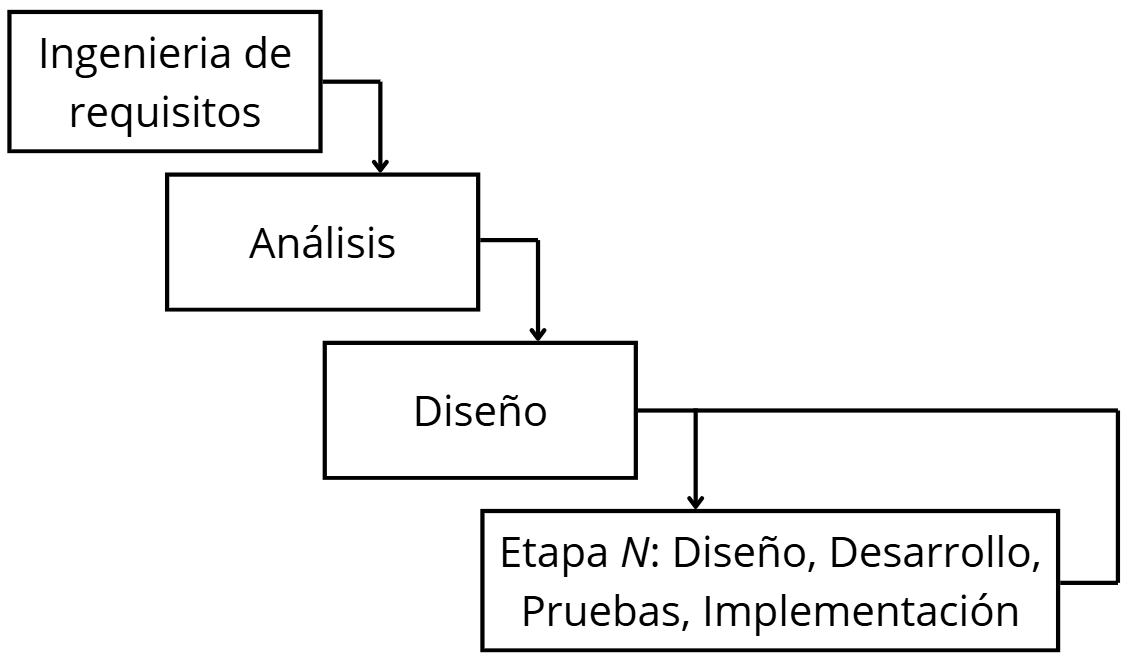
\includegraphics[width=0.75\linewidth]{img/modelo_etapas.png}
	\caption{Representación gráfica del modelo de entrega por etapas para el desarrollo del software}
	\label{fig:modelo_etapas}
\end{figure}

Estas son algunas de las razones por las cuales se opta por este modelo:

\begin{itemize}
	\item El tamaño del equipo de desarrollo es reducido: Al tener un número de integrantes reducido, resulta inviable desarrollar múltiples componentes de forma paralela. 
	
	\item No existe un cliente: El desarrollo de este producto de software es únicamente un medio para el proceso experimental.
	
	\item No es un producto comercial: No se planea monetizar dado que no existe un cliente. Por lo que en la ingeniería de requisitos se consideran los necesarios propuestos por el equipo de investigación para satisfacer las necesidades tecnológicas.
	
	\item No hay procesos iterativos: Al no tener cliente, no es necesario tener una validación externa, ni cambios significativos en los requerimientos del software. 
\end{itemize}

\begin{itemize}
	\item Simulador funcional de cualquier autómata celular en dos dimensiones en un espacio celular finito.
	
	\item Personalización de la vecindad, conjunto de estados, condición de frontera y función de transición.
	
	\item Personalización del diseño de estados e interacción en tiempo real con el espacio celular.
	
	\item Controles de simulación para avanzar, retroceder, reiniciar y manipular la velocidad de la animación.
\end{itemize}

Para mayor detalle de esta primera etapa, más adelante se especifican los casos de uso.

\section{Reglas de negocio}

\begin{enumerate}[label*=RN\arabic*]
	
	\item El estado de una célula en el tiempo $t + 1$ depende únicamente de su estado actual y de los estados de sus vecinos.
	
	\item Para iniciar la simulación es necesario que el conjunto de estados, la topología de la vecindad, la condición de frontera y la función de transición hayan sido definidos.
	
	\item Cuando la simulación está en curso, no se puede cambiar el conjunto de estados, la topología de la vecindad ni la función de transición.
	
	\item El usuario puede manipular el estado de una célula y la condición de frontera en tiempo de ejecución.
	
	\item Los datos importados deben cumplir con el formato definido por el sistema para garantizar su correcta interpretación.
	
	\item Los datos exportados deben conservar el mismo formato que los datos importados.
	
	\item El usuario puede pausar, detener, reanudar o retroceder la simulación sin pérdida de información. 
	
	\item Solo se permite una simulación activa por sesión.
	
\end{enumerate}

\section{Requerimientos}

\subsection{Requerimientos funcionales}

Los requerimientos funcionales describen las capacidades que el sistema debe ofrecer al usuario para cumplir con los objetivos establecidos.

\begin{enumerate}[label=RF\arabic*]
	
	\item El sistema debe mostrar una cuadrícula regular y finita que represente el espacio celular.
	
	\item El sistema debe permitir al usuario interactuar con el espacio celular, asignando o modificando los estados de las células.
	
	\item El sistema debe permitir al usuario definir el conjunto de estados, la topología de la vecindad local y las condiciones de frontera del espacio celular.
	
	\item El sistema debe permitir la evolución del espacio celular mediante un único paso o de forma continua, ajustando la velocidad de actualización según las capacidades computacionales del sistema.
	
	\item El sistema debe permitir la importación y exportación de configuraciones y evoluciones del espacio celular.
	
	\item El sistema debe permitir al usuario establecer la función de transición de manera manual.
	
	\item El sistema debe permitir configurar la red neuronal para imitar el comportamiento de una evolución señalada.
	
	\item El sistema debe entrenar una red neuronal dados los parámetros del usuario y la evolución que desea replicar.
	
\end{enumerate}

\subsection{Requerimientos no funcionales}

Los requerimientos no funcionales especifican las condiciones de calidad, desempeño y compatibilidad bajo las cuales el sistema debe operar.

\begin{enumerate}[label=RNF\arabic*.]
	
	\item El sistema debe poder ejecutarse en Fedora 42 sin requerir modificaciones en el código fuente.
	
	\item El sistema debe ser capaz de procesar al menos 10,000 células o registros por segundo utilizando una GPU NVIDIA RTX 5080.
	
	\item El sistema debe garantizar disponibilidad continua durante la ejecución, sin fallos o interrupciones críticas.
	
	\item La interfaz del sistema debe tener mensajes claros y funcionalidades bien definidas.
	
\end{enumerate}

\subsection{Requerimientos de sistema}

\subsubsection{Recomendado}

Los siguientes requerimientos describen el entorno principal y recomendado de ejecución, en el cual el sistema garantiza un rendimiento óptimo y estabilidad durante los procesos de simulación:

\begin{itemize}
	
	\item \textbf{Procesador:} Intel Core i9-14900K × 32 núcleos.
	
	\item \textbf{GPU:} NVIDIA GeForce RTX 5080.
	
	\item \textbf{Sistema operativo:} Fedora Linux 42 (Workstation Edition).
	
	\item \textbf{Entorno de escritorio:} GNOME 48.
	
	\item \textbf{Sistema de ventaneo:} Wayland.
	
\end{itemize}

\subsubsection{Mínimo}

También se establecen los requisitos mínimos necesarios para usar el simulador, teniendo en cuenta que el rendimiento y la velocidad de procesamiento dependerán de las capacidades del hardware disponible y que el entrenamiento podría no ser posible.

\begin{itemize}
	
	\item \textbf{Procesador:} Intel Core i7-1185G7 × 4 núcleos.
	
	\item \textbf{GPU:} Intel Corporation Raptor Lake-S GT1 [UHD Graphics 770].
	
	\item \textbf{Sistema operativo:} Fedora Linux 42 (Workstation Edition).
	
	\item \textbf{Entorno de escritorio:} GNOME 48.
	
	\item \textbf{Sistema de ventaneo:} Wayland.
	
\end{itemize}
	\section{Análisis de riesgos}

El análisis de riesgos se realiza tomando en cuenta el tiempo estimado de desarrollo de aproximadamente 6 meses, los recursos disponibles para el desarrollo tecnológico y las habilidades técnicas para el diseño de simuladores de autómatas celulares, cómputo paralelo, redes neuronales y programación orientada a eventos. 

\subsection{Identificación de riesgos}

Los riesgos se agrupan en cinco categorías según su origen: técnicos, operativos, de requerimientos, de estimación y de alcance. A cada riesgo se le asigna un código formado por las iniciales de su categoría y un número consecutivo, el cual se utiliza en el resto del análisis.

\subsubsection{Riesgos técnicos}

\begin{enumerate}[label*=RT\arabic*, noitemsep]
	\item Incompatibilidad entre diferentes lenguajes de programación: Los módulos desarrollados en Python, C++ y CUDA generan errores de integración al intercambiar información y sincronizar procesos.
	
	\item Indisponibilidad de \textit{hardware}: La tarjeta gráfica, el procesador u otros componentes no tienen el rendimiento suficiente.
	
	\item Incompatibilidad entre tecnologías: El sistema operativo, los lenguajes de programación y los elementos de \textit{hardware} no son compatibles para el desarrollo y ejecución.
	
	\item Dependencias de bibliotecas: La instalación y configuración de diferentes bibliotecas varía según el sistema operativo.
	
	\item Mala visualización: El renderizado de los componentes gráficos es incorrecto o está mal optimizado.
	
	\item Indisponibilidad de \textit{software} con licencia: Las herramientas que requieren una licencia, como Wolfram Mathematica, dejan de estar disponibles durante el desarrollo por la cancelación o el vencimiento de la licencia.
\end{enumerate}

\subsubsection{Riesgos operativos}
\begin{enumerate}[label*=RO\arabic*, noitemsep]
	\item Documentación deficiente: La documentación no permite mantener ni ampliar el proyecto a futuro.
	
	\item Problemas personales: Falta de motivación o problemas de salud física o mental se presentan durante el desarrollo.
	
	\item Curva de aprendizaje elevada: Se encuentra una curva de aprendizaje elevada y se carece de experiencia con la tecnología a utilizar.
\end{enumerate}
\subsubsection{Riesgos de requerimientos}
\begin{enumerate}[label*=RR\arabic*, noitemsep]
	\item Requerimientos ambiguos: La definición incompleta o ambigua de los requerimientos puede provocar cambios en etapas avanzadas del desarrollo.
\end{enumerate}

\subsubsection{Riesgos de estimación}
\begin{enumerate}[label*=RE\arabic*, noitemsep]
	\item Subestimación del tiempo de desarrollo: La complejidad de enlazar diferentes tecnologías puede extender los plazos planeados.
\end{enumerate}

\subsubsection{Riesgos de alcance}
\begin{enumerate}[label*=RA\arabic*, noitemsep]
	\item Limitación del alcance funcional: Las restricciones de tiempo pueden dar pie a limitar el número de funcionalidades requeridas.

	\item Carga de trabajo imprevista: El poder de cómputo resulta insuficiente, por lo que se reduce la complejidad de las simulaciones.
\end{enumerate}

\subsection{Probabilidad e impacto}

El nivel de cada riesgo se obtiene a partir de dos factores. La probabilidad es la posibilidad de que el riesgo ocurra durante el desarrollo y se clasifica en cinco niveles: muy poco probable (10\%), poco probable (30\%), moderadamente probable (50\%), probable (70\%) y muy probable (90\%). El impacto, o severidad, es la magnitud del daño que causaría al proyecto en caso de ocurrir y se clasifica en nulo, menor, moderado, crítico y fatal. La matriz de riesgos de la tabla \ref{table:matriz_riesgos} combina ambos factores y asigna a cada riesgo un nivel bajo, medio, alto o muy alto \cite{matriz_riesgos}. Siguiendo dicha tabla, en las tablas \ref{table:riesgos_tecnicos} a \ref{table:riesgos_alcance} se enlistan los niveles de riesgo para cada riesgo identificado.

\begin{table}[H]
	\centering
	\renewcommand{\arraystretch}{1.2}
	\setlength{\tabcolsep}{3pt}
	\begin{tabular}{|>{\centering\arraybackslash}m{0.04\textwidth}|p{0.13\textwidth}|*{5}{>{\centering\arraybackslash}p{0.14\textwidth}|}}
		\hhline{~~|-----|}
		\multicolumn{2}{c|}{} & \multicolumn{5}{c|}{\textbf{Probabilidad}} \\ \hhline{~~|-----|}
		\multicolumn{2}{c|}{} & Muy poco probable $10\%$ & Poco probable $30\%$ &  Moderada-mente $50\%$ & Probable $70\%$ & Muy probable $90\%$ \\ \hhline{|-------|}
		\multirow{5}{*}{\rotatebox[origin=c]{90}{\textbf{Severidad}}}
		& Nula & \cellcolor{riskLow}Bajo & \cellcolor{riskLow}Bajo & \cellcolor{riskLow}Bajo & \cellcolor{riskMedium}Medio & \cellcolor{riskMedium}Medio \\ \hhline{|~|------|}
		& Menor & \cellcolor{riskLow}Bajo & \cellcolor{riskLow}Bajo & \cellcolor{riskMedium}Medio & \cellcolor{riskMedium}Medio & \cellcolor{riskMedium}Medio \\ \hhline{|~|------|}
		& Moderado & \cellcolor{riskMedium}Medio & \cellcolor{riskMedium}Medio & \cellcolor{riskMedium}Medio & \cellcolor{riskHigh}Alto & \cellcolor{riskHigh}Alto \\ \hhline{|~|------|}
		& Crítico & \cellcolor{riskMedium}Medio & \cellcolor{riskMedium}Medio & \cellcolor{riskHigh}Alto & \cellcolor{riskHigh}Alto & \cellcolor{riskVeryHigh}Muy alto \\ \hhline{|~|------|}
		& Fatal & \cellcolor{riskMedium}Medio & \cellcolor{riskHigh}Alto & \cellcolor{riskHigh}Alto & \cellcolor{riskVeryHigh}Muy alto & \cellcolor{riskVeryHigh}Muy alto \\ \hhline{|-------|}
	\end{tabular}
	\caption{Matriz de riesgos \cite{matriz_riesgos}}
	\label{table:matriz_riesgos}
\end{table}

\subsection{Plan de mitigación}

El plan de mitigación define, para cada riesgo identificado, las acciones preventivas que se realizan durante el desarrollo para reducir la probabilidad de que ocurra o su impacto. Las tablas \ref{table:riesgos_tecnicos} a \ref{table:riesgos_alcance} presentan, por categoría, el código y el nombre de cada riesgo junto con su plan de mitigación.

\begingroup
\renewcommand{\arraystretch}{1.2}
\setlength{\tabcolsep}{2.5pt}
\begin{longtable}{|>{\raggedright\arraybackslash}p{0.13\textwidth}|p{0.125\textwidth}|p{0.19\textwidth}|>{\raggedright\arraybackslash}p{0.26\textwidth}|p{0.105\textwidth}|p{0.11\textwidth}|}
	\endfirsthead
	\hline
	\endhead
		\hline
		\textbf{RT1} & \riskSpan{Incompatibilidad entre diferentes lenguajes de programación} \\* \hhline{|------|}\noalign{\nobreak}
		\textbf{Impacto:} & Crítico & \textbf{Probabilidad:} & Moderadamente & \textbf{Riesgo:} & \cellcolor{riskHigh}Alto \\* \hhline{|------|}\noalign{\nobreak}
		\textbf{Plan de mitigación:} & \riskSpan{Verificar la documentación de compatibilidad entre los lenguajes de programación y realizar pruebas de transferencia de datos y sincronización previas al desarrollo.} \\* \noalign{\hrule height 1pt}\noalign{\penalty0}
		\textbf{RT2} & \riskSpan{Indisponibilidad de \textit{hardware}} \\* \hhline{|------|}\noalign{\nobreak}
		\textbf{Impacto:} & Moderado & \textbf{Probabilidad:} & Poco probable & \textbf{Riesgo:} & \cellcolor{riskMedium}Medio \\* \hhline{|------|}\noalign{\nobreak}
		\textbf{Plan de mitigación:} & \riskSpan{Asegurar la disponibilidad de equipos de respaldo o entornos virtuales alternativos para continuar el desarrollo en caso de fallos de \textit{hardware}.} \\* \noalign{\hrule height 1pt}\noalign{\penalty0}
		\textbf{RT3} & \riskSpan{Incompatibilidad entre tecnologías} \\* \hhline{|------|}\noalign{\nobreak}
		\textbf{Impacto:} & Fatal & \textbf{Probabilidad:} & Probable & \textbf{Riesgo:} & \cellcolor{riskVeryHigh}Muy alto \\* \hhline{|------|}\noalign{\nobreak}
		\textbf{Plan de mitigación:} & \riskSpan{Realizar pruebas de compatibilidad del \textit{hardware} y \textit{software} en diferentes sistemas operativos y versiones antes de la integración.} \\* \noalign{\hrule height 1pt}\noalign{\penalty0}
		\textbf{RT4} & \riskSpan{Dependencias de bibliotecas} \\* \hhline{|------|}\noalign{\nobreak}
		\textbf{Impacto:} & Menor & \textbf{Probabilidad:} & Poco probable & \textbf{Riesgo:} & \cellcolor{riskLow}Bajo \\* \hhline{|------|}\noalign{\nobreak}
		\textbf{Plan de mitigación:} & \riskSpan{Documentar y verificar las versiones de bibliotecas utilizadas, además de considerar alternativas equivalentes que garanticen continuidad en caso de incompatibilidad.} \\* \noalign{\hrule height 1pt}\noalign{\penalty0}
		\textbf{RT5} & \riskSpan{Mala visualización} \\* \hhline{|------|}\noalign{\nobreak}
		\textbf{Impacto:} & Menor & \textbf{Probabilidad:} & Moderadamente & \textbf{Riesgo:} & \cellcolor{riskMedium}Medio \\* \hhline{|------|}\noalign{\nobreak}
		\textbf{Plan de mitigación:} & \riskSpan{Realizar pruebas de usabilidad y ajustar la interfaz de acuerdo con las resoluciones de pantalla y dispositivos objetivo.} \\* \noalign{\hrule height 1pt}\noalign{\penalty0}
		\textbf{RT6} & \riskSpan{Indisponibilidad de \textit{software} con licencia} \\* \hhline{|------|}\noalign{\nobreak}
		\textbf{Impacto:} & Crítico & \textbf{Probabilidad:} & Muy probable & \textbf{Riesgo:} & \cellcolor{riskVeryHigh}Muy alto \\* \hhline{|------|}\noalign{\nobreak}
		\textbf{Plan de mitigación:} & \riskSpan{Verificar la vigencia de las licencias al inicio del proyecto, limitar el uso de las herramientas con licencia a tareas que no formen parte del simulador y mantener alternativas de \textit{software} libre, como Python, para las tareas de análisis.} \\ \hline
	\caption{Nivel y plan de mitigación de los riesgos técnicos}
	\label{table:riesgos_tecnicos}
\end{longtable}
\endgroup

\begingroup
\renewcommand{\arraystretch}{1.2}
\setlength{\tabcolsep}{2.5pt}
\begin{longtable}{|>{\raggedright\arraybackslash}p{0.13\textwidth}|p{0.125\textwidth}|p{0.19\textwidth}|>{\raggedright\arraybackslash}p{0.26\textwidth}|p{0.105\textwidth}|p{0.11\textwidth}|}
	\endfirsthead
	\hline
	\endhead
		\hline
		\textbf{RO1} & \riskSpan{Documentación deficiente} \\* \hhline{|------|}\noalign{\nobreak}
		\textbf{Impacto:} & Moderado & \textbf{Probabilidad:} & Probable & \textbf{Riesgo:} & \cellcolor{riskHigh}Alto \\* \hhline{|------|}\noalign{\nobreak}
		\textbf{Plan de mitigación:} & \riskSpan{Establecer un estándar de documentación y realizar revisiones periódicas del avance para garantizar la calidad y completitud de los registros técnicos.} \\* \noalign{\hrule height 1pt}\noalign{\penalty0}
		\textbf{RO2} & \riskSpan{Problemas personales} \\* \hhline{|------|}\noalign{\nobreak}
		\textbf{Impacto:} & Crítico & \textbf{Probabilidad:} & Moderadamente & \textbf{Riesgo:} & \cellcolor{riskHigh}Alto \\* \hhline{|------|}\noalign{\nobreak}
		\textbf{Plan de mitigación:} & \riskSpan{Definir roles de respaldo o distribuir responsabilidades para minimizar el impacto de ausencias o contratiempos personales.} \\* \noalign{\hrule height 1pt}\noalign{\penalty0}
		\textbf{RO3} & \riskSpan{Curva de aprendizaje elevada} \\* \hhline{|------|}\noalign{\nobreak}
		\textbf{Impacto:} & Moderado & \textbf{Probabilidad:} & Muy probable & \textbf{Riesgo:} & \cellcolor{riskHigh}Alto \\* \hhline{|------|}\noalign{\nobreak}
		\textbf{Plan de mitigación:} & \riskSpan{Programar capacitaciones iniciales y establecer un periodo de adaptación con apoyo técnico y materiales de referencia.} \\ \hline
	\caption{Nivel y plan de mitigación de los riesgos operativos}
	\label{table:riesgos_operativos}
\end{longtable}
\endgroup

\begingroup
\renewcommand{\arraystretch}{1.2}
\setlength{\tabcolsep}{2.5pt}
\begin{longtable}{|>{\raggedright\arraybackslash}p{0.13\textwidth}|p{0.125\textwidth}|p{0.19\textwidth}|>{\raggedright\arraybackslash}p{0.26\textwidth}|p{0.105\textwidth}|p{0.11\textwidth}|}
	\endfirsthead
	\hline
	\endhead
		\hline
		\textbf{RR1} & \riskSpan{Requerimientos ambiguos} \\* \hhline{|------|}\noalign{\nobreak}
		\textbf{Impacto:} & Menor & \textbf{Probabilidad:} & Poco probable & \textbf{Riesgo:} & \cellcolor{riskLow}Bajo \\* \hhline{|------|}\noalign{\nobreak}
		\textbf{Plan de mitigación:} & \riskSpan{Revisar periódicamente los requerimientos para aclararlos y validar el entendimiento del equipo de desarrollo.} \\ \hline
	\caption{Nivel y plan de mitigación de los riesgos de requerimientos}
	\label{table:riesgos_requerimientos}
\end{longtable}
\endgroup

\begingroup
\renewcommand{\arraystretch}{1.2}
\setlength{\tabcolsep}{2.5pt}
\begin{longtable}{|>{\raggedright\arraybackslash}p{0.13\textwidth}|p{0.125\textwidth}|p{0.19\textwidth}|>{\raggedright\arraybackslash}p{0.26\textwidth}|p{0.105\textwidth}|p{0.11\textwidth}|}
	\endfirsthead
	\hline
	\endhead
		\hline
		\textbf{RE1} & \riskSpan{Subestimación del tiempo de desarrollo} \\* \hhline{|------|}\noalign{\nobreak}
		\textbf{Impacto:} & Fatal & \textbf{Probabilidad:} & Probable & \textbf{Riesgo:} & \cellcolor{riskVeryHigh}Muy alto \\* \hhline{|------|}\noalign{\nobreak}
		\textbf{Plan de mitigación:} & \riskSpan{Dividir el proyecto en fases pequeñas y manejables, aplicando seguimiento semanal y reajuste de cronograma según los resultados obtenidos.} \\ \hline
	\caption{Nivel y plan de mitigación de los riesgos de estimación}
	\label{table:riesgos_estimacion}
\end{longtable}
\endgroup

\begingroup
\renewcommand{\arraystretch}{1.2}
\setlength{\tabcolsep}{2.5pt}
\begin{longtable}{|>{\raggedright\arraybackslash}p{0.13\textwidth}|p{0.125\textwidth}|p{0.19\textwidth}|>{\raggedright\arraybackslash}p{0.26\textwidth}|p{0.105\textwidth}|p{0.11\textwidth}|}
	\endfirsthead
	\hline
	\endhead
		\hline
		\textbf{RA1} & \riskSpan{Limitación del alcance funcional} \\* \hhline{|------|}\noalign{\nobreak}
		\textbf{Impacto:} & Moderado & \textbf{Probabilidad:} & Moderadamente & \textbf{Riesgo:} & \cellcolor{riskMedium}Medio \\* \hhline{|------|}\noalign{\nobreak}
		\textbf{Plan de mitigación:} & \riskSpan{Definir claramente los objetivos y alcances desde el inicio, con aprobación formal de los responsables del proyecto antes de iniciar nuevas funcionalidades.} \\* \noalign{\hrule height 1pt}\noalign{\penalty0}
		\textbf{RA2} & \riskSpan{Carga de trabajo imprevista} \\* \hhline{|------|}\noalign{\nobreak}
		\textbf{Impacto:} & Crítico & \textbf{Probabilidad:} & Probable & \textbf{Riesgo:} & \cellcolor{riskHigh}Alto \\* \hhline{|------|}\noalign{\nobreak}
		\textbf{Plan de mitigación:} & \riskSpan{Implementar revisiones periódicas del plan de trabajo y ajustar el alcance en función de los recursos disponibles y los resultados obtenidos.} \\ \hline
	\caption{Nivel y plan de mitigación de los riesgos de alcance}
	\label{table:riesgos_alcance}
\end{longtable}
\endgroup

\subsection{Plan de contingencia}

El plan de contingencia define las acciones que se ejecutan cuando un riesgo se materializa a pesar de las medidas de mitigación. Se elabora únicamente para los riesgos de nivel muy alto, que son los siguientes:
\begin{itemize}
	\item \textbf{RT3} Incompatibilidad entre tecnologías.
	\item \textbf{RT6} Indisponibilidad de \textit{software} con licencia.
	\item \textbf{RE1} Subestimación del tiempo de desarrollo. 
\end{itemize}

Para cada uno se indican su probabilidad, su impacto, el plan de evasión (acciones para evitar que el riesgo ocurra) y las acciones de contingencia (qué hacer cuando ocurre).

\subsubsection{RT3 Incompatibilidad entre tecnologías}

\begin{table}[H]
	\centering
	\renewcommand{\arraystretch}{1.2}
	\setlength{\tabcolsep}{2.5pt}
	\begin{tabular}{|>{\raggedright\arraybackslash}p{0.13\textwidth}|p{0.09\textwidth}|p{0.19\textwidth}|>{\raggedright\arraybackslash}p{0.295\textwidth}|p{0.105\textwidth}|p{0.11\textwidth}|}
		\hline
		\textbf{RT3} & \riskSpan{Incompatibilidad entre tecnologías} \\ \hhline{|------|}
		\textbf{Impacto:} & Fatal & \textbf{Probabilidad:} & Probable (70\%) & \textbf{Riesgo:} & \cellcolor{riskVeryHigh}Muy alto \\ \hhline{|------|}
		\textbf{Plan de evasión:} & \riskSpan{Realizar pruebas de integración tempranas entre las distintas tecnologías implicadas. Documentar las versiones, dependencias y configuraciones utilizadas para garantizar compatibilidad. Establecer un entorno de desarrollo unificado que minimice diferencias entre plataformas.} \\ \hhline{|------|}
		\textbf{Plan de contingencia:} & \riskSpan{Sustituir o actualizar los componentes que generen incompatibilidad. Implementar adaptadores o módulos intermedios que permitan la interoperabilidad entre sistemas. Reasignar recursos técnicos para resolver los conflictos de integración y evitar retrasos prolongados.} \\ \hline
	\end{tabular}
	\caption{Plan de contingencia para RT3 Incompatibilidad entre tecnologías}
	\label{table:contingencia_incompatibilidad}
\end{table}

\subsubsection{RT6 Indisponibilidad de software con licencia}

\begin{table}[H]
	\centering
	\renewcommand{\arraystretch}{1.2}
	\setlength{\tabcolsep}{2.5pt}
	\begin{tabular}{|>{\raggedright\arraybackslash}p{0.13\textwidth}|p{0.09\textwidth}|p{0.19\textwidth}|>{\raggedright\arraybackslash}p{0.295\textwidth}|p{0.105\textwidth}|p{0.11\textwidth}|}
		\hline
		\textbf{RT6} & \riskSpan{Indisponibilidad de \textit{software} con licencia} \\ \hhline{|------|}
		\textbf{Impacto:} & Crítico & \textbf{Probabilidad:} & Muy probable (90\%) & \textbf{Riesgo:} & \cellcolor{riskVeryHigh}Muy alto \\ \hhline{|------|}
		\textbf{Plan de evasión:} & \riskSpan{Verificar al inicio del proyecto la vigencia y las condiciones de renovación de cada licencia. Mantener el simulador independiente de las herramientas con licencia, de modo que estas solo se usen para el análisis de resultados. Preparar alternativas de \textit{software} libre (NumPy, Matplotlib y Scikit-learn) para las tareas de análisis.} \\ \hhline{|------|}
		\textbf{Plan de contingencia:} & \riskSpan{Adquirir una licencia individual por el tiempo restante del proyecto. Migrar los cuadernos de análisis a las alternativas de \textit{software} libre si no es posible adquirir la licencia. Reajustar el cronograma para absorber el tiempo de migración.} \\ \hhline{|------|}
	\end{tabular}
	\caption{Plan de contingencia para RT6 Indisponibilidad de \textit{software} con licencia}
	\label{table:contingencia_licencia}
\end{table}

\subsubsection{RE1 Subestimación del tiempo de desarrollo}

\begin{table}[H]
	\centering
	\renewcommand{\arraystretch}{1.2}
	\setlength{\tabcolsep}{2.5pt}
	\begin{tabular}{|>{\raggedright\arraybackslash}p{0.13\textwidth}|p{0.09\textwidth}|p{0.19\textwidth}|>{\raggedright\arraybackslash}p{0.295\textwidth}|p{0.105\textwidth}|p{0.11\textwidth}|}
		\hline
		\textbf{RE1} & \riskSpan{Subestimación del tiempo de desarrollo} \\ \hhline{|------|}
		\textbf{Impacto:} & Fatal & \textbf{Probabilidad:} & Probable (70\%) & \textbf{Riesgo:} & \cellcolor{riskVeryHigh}Muy alto \\ \hhline{|------|}
		\textbf{Plan de evasión:} & \riskSpan{Realizar estimaciones realistas basadas en experiencias previas y tareas medibles. Incluir márgenes de tiempo de reserva en el cronograma para absorber imprevistos. Efectuar reuniones de seguimiento semanales para detectar desviaciones tempranas.} \\ \hhline{|------|}
		\textbf{Plan de contingencia:} & \riskSpan{Reasignar recursos o personal adicional para recuperar el tiempo perdido. Reducir temporalmente el alcance funcional o posponer características no críticas. Reajustar el cronograma de entregas y comunicar los cambios al equipo y partes interesadas.} \\ \hline
	\end{tabular}
	\caption{Plan de contingencia para RE1 Subestimación del tiempo de desarrollo}
	\label{table:contingencia_subestimacion}
\end{table}

\section{Estudio de factibilidad}

El proyecto cuenta con los recursos de \textit{hardware} necesarios para llevar a cabo simulaciones de alto nivel computacional. El equipo de cómputo disponible permite implementar técnicas de paralelización, asegurando la capacidad de realizar múltiples inferencias en tiempos razonables. Adicionalmente, se dispone de herramientas tecnológicas de alto rendimiento que brindan la ventaja computacional requerida para ejecutar la simulación de manera eficiente.

En cuanto a la factibilidad económica, la mayor parte del \textit{software} utilizado es de libre acceso, incluyendo Python, C++, Visual Studio Code y TeXstudio. Se utiliza también Wolfram Mathematica, que requiere una licencia anual de 195 dólares, la cual se encontraba disponible de manera gratuita para estudiantes del IPN al inicio del proyecto. Al cancelarse dicha licencia se adquirió una licencia de estudiante por un año (ver el plan de contingencia del riesgo RT6), un costo que no compromete la viabilidad financiera del proyecto.

Desde el punto de vista operativo, el diseño de la interfaz facilita la definición de reglas y la ejecución de simulaciones, optimizando el flujo de trabajo del grupo de investigadores. Esto permite acelerar significativamente el proceso de experimentación y análisis de resultados, maximizando la eficiencia del equipo durante el desarrollo del proyecto.

Finalmente, se cumple la factibilidad temporal, ya que el cronograma de desarrollo estimado permite realizar todas las simulaciones necesarias para el análisis posterior, asegurando que el proyecto se pueda completar dentro del tiempo previsto.



	\section{Casos de uso}

\begin{figure}[H]
	\centering
	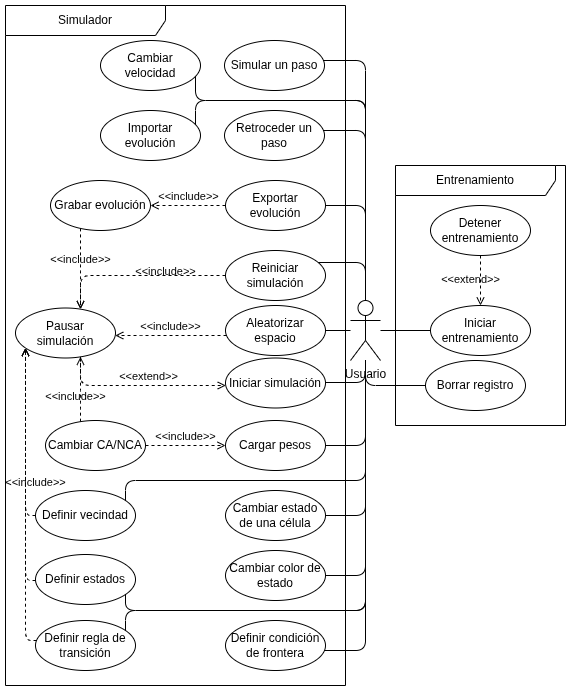
\includegraphics[width=0.95\linewidth]{img/uml_ucd.png}
	\caption{Diagrama de casos de uso}
	\label{fig:uml_ucd}
\end{figure}


\section{Diccionario}

\subsection{Interfaces gráficas}
\begin{itemize}
	\item \NewUI{control_ui}{Control}: Elemento que contiene los botones de control sobre la simulación del espacio celular.
	\item \NewUI{simulacion_ui}{Simulación}: Elemento que contiene la cuadrícula del espacio celular y muestra la evolución del autómata celular.
	\item \NewUI{configuracion_ui}{Configuración}: Elemento que permite realizar la configuración de la vecindad, condición de frontera, estados y función de transición.
	\item \NewUI{training_ui}{Entrenamiento}: Contiene la personalización del entrenamiento del autómata celular neuronal.
\end{itemize}

\subsection{Entradas}
\begin{itemize}	
	% Configuración
	\item Controles de simulación:
	\begin{itemize}
		\item \NewBTN{iniciar_simulacion}{Iniciar simulación}
		\item \NewBTN{pausar_simulacion}{Pausar simulación}
		\item \NewBTN{paso_adelante}{Simular un paso}
		\item \NewBTN{paso_atras}{Retroceder un paso}
		\item \NewBTN{reiniciar_simulacion}{Reiniciar simulación}
		\item \NewBTN{aleatorizar_simulacion}{Aleatorizar espacio}
		
		\item \NewBTN{importar}{Importar evolución}
		\item \NewBTN{grabar_evolucion}{Grabar evolución}
		\item \NewBTN{exportar}{Exportar evolución}
		
		\item \NewBTN{cargar_pesos}{Cargar pesos}
		\item \NewBTN{cambiar_ca_nca}{Cambiar CA/NCA}
	
		\item \NewSLD{velocidad}{Cambiar velocidad}
		\item \NewSLD{paso}{Eligir paso}
	
		\item \NewIN{grabar_pasos}{Numero de pasos}
	
		\item \NewMSG{formato_incorrecto}{Formato de archivo incorrecto}

		\item \NewMSG{tamaño_incorrecto}{Tamaño incorrecto}
		\item \NewMSG{evolucion_vacia}{Sin evolución}
	\end{itemize}
	
	\item Configuración del autómata celular:
	\begin{itemize}
		\item \NewBTN{def_vecindad}{Definir vecindad}
		\item \NewBTN{añadir_grupo}{Añadir grupo}
		\item \NewBTN{eliminar_grupo}{Eliminar grupo}
		
		\item \NewBTN{def_estados}{Definir estados}		
		\item \NewBTN{estado}{Estado $n$-esimo.}		

		\item \NewBTN{def_frontera}{Definir condición de frontera}
		
		\item \NewBTN{def_regla}{Definir regla}
		
		\item \NewIN{grupo_vecindad}{Grupo de vecindad}
		\item \NewIN{espacio_vecindad}{Espacio vecindad}
		
		\item \NewIN{estados}{Estados}		
		
		\item \NewIN{regla}{Regla}
		\item \NewIN{regla_codigo}{Regla (Código)}
	\end{itemize}
	
	\item Espacio de simulación:
	\begin{itemize}
		\item \NewIN{espacio}{Espacio}
	\end{itemize}
	
	\item Entrenamiento del automata celular neuronal:
	\begin{itemize}
		\item \NewBTN{cargar_evolucion}{Cargar evolución}
		\item \NewBTN{definir_guardado}{Definir ruta de guardado}
		
		\item \NewBTN{entrenar}{Iniciar entrenamiento}
		\item \NewBTN{detener}{Detener entrenamiento}
	
		\item \NewIN{entrenamiento_vecindad}{Vecindad}
		\item \NewIN{capas_ocultas}{Capas ocultas}
		\item \NewIN{neuronas}{Neuronas}
		\item \NewIN{relu}{Activación ReLU}
		\item \NewIN{sigmoid}{Activación sigmoide}
		\item \NewIN{tanh}{Activación Tanh}
		\item \NewIN{lineal}{Activación lineal}
		\item \NewIN{salida}{Capa de salida}
		\item \NewIN{funcion_salida}{Ultima función de activación}
		\item \NewIN{epocas}{Epocas}
		\item \NewIN{tamaño_lote}{Tamaño de lotes}
		\item \NewIN{tasa_aprendizaje}{Tasa de aprendizaje}
		\item \NewIN{perdida_objetivo}{Perdida objetivo}
		\item \NewIN{imprimir}{Imprimir cada N}
		
		\item \NewIN{borrar_consola}{Borrar consola}
		
		\item \NewMSG{entrenamiento_incompleto}{Entrenamiento incompleto}
		
		\item \NewOUT{ruta_in}{Ruta de evolución}
		\item \NewOUT{ruta_out}{Ruta de guardado}
		\item \NewOUT{entrenamiento_vecindad_mapa}{Mapa de vecindad}
		\item \NewOUT{consola}{Consola}
	\end{itemize}
\end{itemize}
	\section{Especificaciones de casos de uso}

\subsection{Controles de simulación}

Los siguientes casos de uso permiten al usuario controlar la evolución del autómata celular. Esto implica evolucionar el sistema hacia adelante, hacia atrás y definiendo velocidades.

\subsubsection*{UC01 Iniciar simulación}

\begin{table}[H]
\begin{center}
	\begin{tabular}{| p{0.2\textwidth} | p{0.7\textwidth} |}
		\hline 
			\textbf{Actor} & Usuario. \\ \hline
			\textbf{Descripción} & El sistema inicia la evolución en pasos de tiempo constante. \\ \hline
			\textbf{Tipo} & Primario. \\ \hline
			\textbf{Entradas} &
			\begin{itemize}[noitemsep, nosep]
			\item Desde mouse \BTN{iniciar_simulacion}.
				\end{itemize}
			\\ \hline
			\textbf{Salidas} & Ninguna. \\ \hline
			\textbf{Precondición} & \begin{itemize}[noitemsep, nosep]
				\item Simulación detenida.
				\item Botón \BTN{iniciar_simulacion} habilitado.
			\end{itemize}
			\\ \hline
			\textbf{Postcondición} & \begin{itemize}[noitemsep, nosep]
				\item Simulación en ejecución.
				\item Botón \BTN{iniciar_simulacion} deshabilitado.
				\item Botón \BTN{pausar_simulacion} habilitado.
			\end{itemize} \\ \hline
			\textbf{Errores}  & Ninguno.  \\ \hline
			\end{tabular}
		\end{center}
	\end{table}

\begin{table}[H]
\begin{center}
	\begin{tabular}{|p{0.45\textwidth}|p{0.45\textwidth}|}
		\hline
			\multicolumn{2}{|c|}{\textbf{Flujo básico}} \\ \hline
			\textbf{Actor} & \textbf{Sistema} \\
			\hline
			\begin{enumerate}[noitemsep, nosep]
			\item Presiona el botón \BTN{iniciar_simulacion} desde \UI{control_ui}.
				\end{enumerate} 
			& 
			\begin{enumerate}[noitemsep, nosep]
				\item[2.] Deshabilita el botón \BTN{iniciar_simulacion}.
				\item[3.] Habilita el botón \BTN{pausar_simulacion}.
				\item[4.] Inicia la simulación. Cada paso evolutivo se realiza a una velocidad constante. 			
				\item[5.] Precarga evoluciones futuras en una cola.
				\item[6.] Actualiza de forma constante \UI{simulacion_ui} con la evolución del sistema.
				\end{enumerate} \\
			\hline
			\end{tabular} \\
		\end{center}
	\end{table}

\subsubsection*{UC02 Pausar simulación}

\begin{table}[H]
\begin{center}
	\begin{tabular}{| p{0.2\textwidth} | p{0.7\textwidth} |}
		\hline 
			\textbf{Actor} & Usuario. \\ \hline
			\textbf{Descripción} & Se detiene la simulación.  \\ \hline
			\textbf{Tipo} & Secundario. \\ \hline
			\textbf{Entradas} &
			\begin{itemize}[noitemsep, nosep]
			\item Desde mouse \BTN{pausar_simulacion}.
				\end{itemize}
			\\ \hline
			\textbf{Salidas} & Ninguna. \\ \hline
			\textbf{Precondición} &  \begin{itemize}[noitemsep, nosep]
				\item Simulación en ejecución.
				\item Botón \BTN{pausar_simulacion} habilitado.
			\end{itemize}			\\ \hline
			\textbf{Postcondición} & \begin{itemize}[noitemsep, nosep]
				\item Simulación detenida.
				\item Botón \BTN{pausar_simulacion} deshabilitado.
				\item Botón \BTN{iniciar_simulacion} habilitado.
			\end{itemize}  \\ \hline
			\textbf{Errores} & Ninguno. \\ \hline
			\end{tabular}
			\end{center}
				\end{table}
			
		\begin{table}[H]
	\begin{center}
\begin{tabular}{|p{0.45\textwidth}|p{0.45\textwidth}|}
\hline
\multicolumn{2}{|c|}{\textbf{Flujo básico}} \\ \hline
	\textbf{Actor} & \textbf{Sistema} \\
		\hline
			\begin{enumerate}[noitemsep, nosep]
			\item Presiona el botón \BTN{pausar_simulacion} desde \UI{control_ui}.
			\end{enumerate} 
			& 
			\begin{enumerate}[noitemsep, nosep]
				\item[2.] Detiene la simulación en \UI{simulacion_ui}. 
				\item[3.] Deshabilita el botón \BTN{pausar_simulacion}.
				\item[4.] Habilita el botón \BTN{iniciar_simulacion}. 
			\end{enumerate} \\
				\hline
			\end{tabular} \\
			\end{center}
		\end{table}
	
\subsubsection*{UC03 Cambiar velocidad}

\begin{table}[H]
	\begin{center}
		\begin{tabular}{| p{0.2\textwidth} | p{0.7\textwidth} |}
			\hline 
			\textbf{Actor} & Usuario. \\ \hline
			\textbf{Descripción} & Se cambia la velocidad de actualización del autómata celular. \\ \hline
			\textbf{Tipo} & Secundario. \\ \hline
			\textbf{Entradas} &
			\begin{itemize}[noitemsep, nosep]
				\item Desde mouse \SLD{velocidad}.
			\end{itemize}
			\\ \hline
			\textbf{Salidas} & Ninguna. \\ \hline
			\textbf{Precondición} & 
				Ninguna.
			\\ \hline
			\textbf{Postcondición} & \begin{itemize}[noitemsep, nosep]
				\item Cambia la velocidad de simulación.
			\end{itemize}  \\ \hline
			\textbf{Errores} & 
				Ninguno. \\ \hline
			\end{tabular}
	\end{center}
\end{table}

\begin{table}[H]
	\begin{center}
		\begin{tabular}{|p{0.45\textwidth}|p{0.45\textwidth}|}
			\hline
			\multicolumn{2}{|c|}{\textbf{Flujo básico}} \\ \hline
			\textbf{Actor} & \textbf{Sistema} \\
			\hline 
			\begin{enumerate}[noitemsep, nosep]
				\item Presiona \SLD{velocidad} desde \UI{control_ui} y desliza a la velocidad deseada.
			\end{enumerate} 
			& 
			\begin{enumerate}[noitemsep, nosep] 
				\item[2.] Cambia la velocidad de la simulación a la velocidad seleccionada.
			\end{enumerate} \\
			\hline
		\end{tabular} \\
	\end{center}
\end{table}

\subsubsection*{UC04 Simular un paso}

\begin{table}[H]
\begin{center}
\begin{tabular}{| p{0.2\textwidth} | p{0.7\textwidth} |}
	\hline 
		\textbf{Actor} & Usuario. \\ \hline
			\textbf{Descripción} & Se realiza la simulación del CA, pero únicamente en un paso. \\ \hline
			\textbf{Tipo} & Primario. \\ \hline
			\textbf{Entradas} &
			\begin{itemize}[noitemsep, nosep]
			\item Desde mouse \BTN{paso_adelante}.
			\end{itemize}
				\\ \hline
			\textbf{Salidas} & Ninguna. \\ \hline
			\textbf{Precondición} & Ninguna.
			\\ \hline
			\textbf{Postcondición} & \begin{itemize}[noitemsep, nosep]
				\item Evoluciona el sistema.
			\end{itemize}  \\ \hline
			\textbf{Errores} & 
			\begin{itemize}[noitemsep, nosep]
			\item Velocidad máxima: Se intenta dar un paso cuando la simulación está activa en la velocidad máxima.
			\end{itemize}\\ \hline
				\end{tabular}
			\end{center}
		\end{table}
	
\begin{table}[H]
\begin{center}
\begin{tabular}{|p{0.45\textwidth}|p{0.45\textwidth}|}
	\hline
		\multicolumn{2}{|c|}{\textbf{Flujo básico}} \\ \hline
			\textbf{Actor} & \textbf{Sistema} \\
			\hline
			\begin{enumerate}[noitemsep, nosep]
			\item Presiona el botón \BTN{paso_adelante} desde \UI{control_ui}.
			\end{enumerate} 
				& 
			\begin{enumerate}[noitemsep, nosep]
			\item[2.] La simulación avanza un paso.
			\item[3.] Actualiza \UI{simulacion_ui}.
			\end{enumerate} \\
				\hline
			\end{tabular} \\
			\end{center}
		\end{table}
	
\begin{table}[H]
\begin{center}
\begin{tabular}{|p{0.45\textwidth}|p{0.45\textwidth}|}
	\hline
		\multicolumn{2}{|c|}{\textbf{Flujo alterno 1: Velocidad máxima}} \\ \hline
			\textbf{Actor} & \textbf{Sistema} \\
			\hline
			\begin{enumerate}[noitemsep, nosep]
			\item[1.1.] Presiona el botón \BTN{paso_adelante} desde \UI{control_ui} cuando la simulación está activa y la velocidad está en la velocidad máxima.
			\end{enumerate} 
				& 
			\begin{enumerate}[noitemsep, nosep]
			\item[1.2.] Agrega la simulación a una cola y mantiene la velocidad actual. 
			\item[1.3.] Actualiza \UI{simulacion_ui}.
			\end{enumerate} \\
				\hline
			\end{tabular} 
			\end{center}
		\end{table}
		
\subsubsection*{UC05 Retroceder un paso}

\begin{table}[H]
	\begin{center}
		\begin{tabular}{| p{0.2\textwidth} | p{0.7\textwidth} |}
			\hline 
			\textbf{Actor} & Usuario. \\ \hline
			\textbf{Descripción} & El sistema restaura el estado anterior de la simulación. \\ \hline
			\textbf{Tipo} & Secundario. \\ \hline
			\textbf{Entradas} &
			\begin{itemize}[noitemsep, nosep]
				\item Desde mouse \BTN{paso_atras}.
			\end{itemize}
			\\ \hline
			\textbf{Salidas} & Ninguna. \\ \hline
			\textbf{Precondición} & \begin{itemize}[noitemsep, nosep]
				\item Existe un estado previo.
			\end{itemize}
			\\ \hline
			\textbf{Postcondición} & \begin{itemize}[noitemsep, nosep]
				\item El sistema restaura la evolución pasada.
			\end{itemize}  \\ \hline
			\textbf{Errores} & 
			\begin{itemize}[noitemsep, nosep]
				\item Configuración inicial: El usuario intenta retroceder la simulación de la configuración inicial.
			\end{itemize}\\ \hline
		\end{tabular}
	\end{center}
\end{table}

\begin{table}[H]
	\begin{center}
		\begin{tabular}{|p{0.45\textwidth}|p{0.45\textwidth}|}
			\hline
			\multicolumn{2}{|c|}{\textbf{Flujo básico}} \\ \hline
			\textbf{Actor} & \textbf{Sistema} \\
			\hline
			\begin{enumerate}[noitemsep, nosep]
				\item Presiona el botón \BTN{paso_atras} desde \UI{control_ui}.
			\end{enumerate} 
			& 
			\begin{enumerate}[noitemsep, nosep]
				\item[2.] La simulación retrocede un paso. 
				\item[3.] Actualiza \UI{simulacion_ui}. 
			\end{enumerate} \\
			\hline
		\end{tabular} \\
	\end{center}
\end{table}

\begin{table}[H]
	\begin{center}
		\begin{tabular}{|p{0.45\textwidth}|p{0.45\textwidth}|}
			\hline
			\multicolumn{2}{|c|}{\textbf{Flujo alterno 1: Configuración inicial}} \\ \hline
			\textbf{Actor} & \textbf{Sistema} \\
			\hline
			\begin{enumerate}[noitemsep, nosep]
				\item[1.1.] Presiona el botón \BTN{paso_atras} desde \UI{control_ui} estando en la configuración inicial (no hay más configuraciones antes).  
			\end{enumerate}
			& 
			\begin{enumerate}[noitemsep, nosep]
				\item[1.2.] No realiza ningún cambio.
			\end{enumerate} \\
			\hline
		\end{tabular} 
	\end{center}
\end{table}

\subsubsection*{UC06 Reiniciar simulación}

\begin{table}[H]
	\begin{center}
		\begin{tabular}{| p{0.2\textwidth} | p{0.7\textwidth} |}
			\hline 
			\textbf{Actor} & Usuario. \\ \hline
			\textbf{Descripción} & Restablece la simulación a su estado inicial (todas las células vacías). \\ \hline
			\textbf{Tipo} & Secundario. \\ \hline
			\textbf{Entradas} &
			\begin{itemize}[noitemsep, nosep]
				\item Desde mouse \BTN{reiniciar_simulacion}.
			\end{itemize}
			\\ \hline
			\textbf{Salidas} & Ninguna. \\ \hline
			\textbf{Precondición} & Ninguna.
			\\ \hline
			\textbf{Postcondición} & \begin{itemize}[noitemsep, nosep]
				\item El sistema adquiere la configuración nula.
			\end{itemize}  \\ \hline
			\textbf{Errores} & Ninguno. \\ \hline
		\end{tabular}
	\end{center}
\end{table}

\begin{table}[H]
	\begin{center}
		\begin{tabular}{|p{0.45\textwidth}|p{0.45\textwidth}|}
			\hline
			\multicolumn{2}{|c|}{\textbf{Flujo básico}} \\ \hline
			\textbf{Actor} & \textbf{Sistema} \\
			\hline
			\begin{enumerate}[noitemsep, nosep]
				\item Presiona el botón \BTN{reiniciar_simulacion} desde \UI{control_ui}.
			\end{enumerate} 
			& 
			\begin{enumerate}[noitemsep, nosep]
				\item[2.] Regresa la configuración a la última versión modificada mientras estaba en pausa. 
				\item[3.] Elimina el historial de evoluciones.
				\item[4.] Actualiza \UI{simulacion_ui}.
			\end{enumerate} \\
			\hline
		\end{tabular} \\
	\end{center}
\end{table}

\subsubsection*{UC07 Aleatorizar espacio}

\begin{table}[H]
	\begin{center}
		\begin{tabular}{| p{0.2\textwidth} | p{0.7\textwidth} |}
			\hline 
			\textbf{Actor} & Usuario. \\ \hline
			\textbf{Descripción} & Establece una configuración aleatoria en el espacio. \\ \hline
			\textbf{Tipo} & Secundario. \\ \hline
			\textbf{Entradas} &
			\begin{itemize}[noitemsep, nosep]
				\item Desde mouse \BTN{aleatorizar_simulacion}.
			\end{itemize}
			\\ \hline
			\textbf{Salidas} & Ninguna. \\ \hline
			\textbf{Precondición} & Ninguna.
			\\ \hline
			\textbf{Postcondición} & \begin{itemize}[noitemsep, nosep]
				\item El sistema adquiere una configuración aleatoria.
			\end{itemize}  \\ \hline
			\textbf{Errores} & Ninguno. \\ \hline
		\end{tabular}
	\end{center}
\end{table}

\begin{table}[H]
	\begin{center}
		\begin{tabular}{|p{0.45\textwidth}|p{0.45\textwidth}|}
			\hline
			\multicolumn{2}{|c|}{\textbf{Flujo básico}} \\ \hline
			\textbf{Actor} & \textbf{Sistema} \\
			\hline
			\begin{enumerate}[noitemsep, nosep]
				\item Presiona el botón \BTN{aleatorizar_simulacion} desde \UI{control_ui}.
			\end{enumerate} 
			& 
			\begin{enumerate}[noitemsep, nosep]
				\item[2.] La configuración del espacio celular adquiere valores aleatorios según el número de estados definidos.
				\item[3.] Elimina el historial de evoluciones.
				\item[4.] Actualiza \UI{simulacion_ui}.
			\end{enumerate} \\
			\hline
		\end{tabular} \\
	\end{center}
\end{table}

\subsubsection*{UC08 Importar evolución}

\begin{table}[H]
	\begin{center}
		\begin{tabular}{| p{0.2\textwidth} | p{0.7\textwidth} |}
			\hline 
			\textbf{Actor} & Usuario. \\ \hline
			\textbf{Descripción} & Importa una evolución guardada en formato ``npy''. \\ \hline
			\textbf{Tipo} & Secundario. \\ \hline
			\textbf{Entradas} &
			\begin{itemize}[noitemsep, nosep]
				\item Desde mouse \BTN{importar}.
			\end{itemize}
			\\ \hline
			\textbf{Salidas} & \begin{itemize}[noitemsep, nosep]
				\item \MSG{formato_incorrecto}.
				\item \MSG{tamaño_incorrecto}.
			\end{itemize} \\ \hline
			\textbf{Precondición} & Ninguna.
			\\ \hline
			\textbf{Postcondición} & \begin{itemize}[noitemsep, nosep]
				\item El sistema carga la simulación y la muestra en \UI{simulacion_ui}.
			\end{itemize}  \\ \hline
			\textbf{Errores} & \begin{itemize}[noitemsep, nosep]
				\item Formato inválido: El archivo no coincide.
				\item Tamaño no compatible: El tamaño no coincide.
			\end{itemize}  \\ \hline
		\end{tabular}
	\end{center}
\end{table}

\begin{table}[H]
	\begin{center}
		\begin{tabular}{|p{0.45\textwidth}|p{0.45\textwidth}|}
			\hline
			\multicolumn{2}{|c|}{\textbf{Flujo básico}} \\ \hline
			\textbf{Actor} & \textbf{Sistema} \\
			\hline
			\begin{enumerate}[noitemsep, nosep]
				\item Presiona el botón \BTN{importar} desde \UI{control_ui}.
				\item[3. ] Selecciona el archivo ``npy'' que contenga una evolución.
			\end{enumerate} 
			& 
			\begin{enumerate}[noitemsep, nosep]
				\item[2.] Abre el explorador de archivos.
				\item[4.] Carga la evolución.
				\item[5.] Actualiza \UI{simulacion_ui}.
			\end{enumerate} \\
			\hline
		\end{tabular} \\
	\end{center}
\end{table}

\begin{table}[H]
	\begin{center}
		\begin{tabular}{|p{0.45\textwidth}|p{0.45\textwidth}|}
			\hline
			\multicolumn{2}{|c|}{\textbf{Flujo alterno 1: Formato inválido}} \\ \hline
			\textbf{Actor} & \textbf{Sistema} \\
			\hline
			\begin{enumerate}[noitemsep, nosep]
				\item[1.1.] Presiona el botón \BTN{importar} desde \UI{control_ui}.
				\item[1.3. ]   Selecciona un archivo ``npy'' inválido u otro tipo de archivo.
			\end{enumerate}
			& 
			\begin{enumerate}[noitemsep, nosep]
				\item[1.2.] Abre el explorador de archivos.
				\item[1.4.] No realiza ningún cambio y muestra \MSG{formato_incorrecto}.
			\end{enumerate} \\
			\hline
		\end{tabular} 
	\end{center}
\end{table}

\begin{table}[H]
	\begin{center}
		\begin{tabular}{|p{0.45\textwidth}|p{0.45\textwidth}|}
			\hline
			\multicolumn{2}{|c|}{\textbf{Flujo alterno 2: Tamaño no compatible}} \\ \hline
			\textbf{Actor} & \textbf{Sistema} \\
			\hline
			\begin{enumerate}[noitemsep, nosep]
				\item[2.1.] Presiona el botón \BTN{importar} desde \UI{control_ui}.
				\item[2.3. ] Selecciona el archivo ``npy'' que contenga una evolución con un tamaño diferente a \UI{simulacion_ui}.
			\end{enumerate}
			& 
			\begin{enumerate}[noitemsep, nosep]
				\item[2.2.] Abre el explorador de archivos.
				\item[2.4.] Recorta o centra la evolución y muestra el mensaje \MSG{tamaño_incorrecto}.
				\item[2.5.] Actualiza \UI{simulacion_ui}.
			\end{enumerate} \\
			\hline
		\end{tabular} 
	\end{center}
\end{table}

\subsubsection*{UC09 Grabar evolución}

\begin{table}[H]
	\begin{center}
		\begin{tabular}{| p{0.2\textwidth} | p{0.7\textwidth} |}
			\hline 
			\textbf{Actor} & Usuario. \\ \hline
			\textbf{Descripción} & Evoluciona el sistema sin visualización y guarda todos los pasos. \\ \hline
			\textbf{Tipo} & Secundario. \\ \hline
			\textbf{Entradas} &
			\begin{itemize}[noitemsep, nosep]
				\item Desde mouse \BTN{grabar_evolucion}.
				\item Desde teclado \IN{grabar_pasos}.
			\end{itemize}
			\\ \hline
			\textbf{Salidas} & Ninguna. \\ \hline
			\textbf{Precondición} & Ninguna.
			\\ \hline
			\textbf{Postcondición} & \begin{itemize}[noitemsep, nosep]
				\item El sistema evoluciona los pasos seleccionados.
			\end{itemize}  \\ \hline
			\textbf{Errores} & Ninguno. \\ \hline
		\end{tabular}
	\end{center}
\end{table}

\begin{table}[H]
	\begin{center}
		\begin{tabular}{|p{0.45\textwidth}|p{0.45\textwidth}|}
			\hline
			\multicolumn{2}{|c|}{\textbf{Flujo básico}} \\ \hline
			\textbf{Actor} & \textbf{Sistema} \\
			\hline
			\begin{enumerate}[noitemsep, nosep]
				\item Presiona el botón \BTN{grabar_evolucion} desde \UI{control_ui}.
				\item[3. ] Elige un número con \IN{grabar_pasos}.
			\end{enumerate} 
			& 
			\begin{enumerate}[noitemsep, nosep]
				\item[2.] Abre una ventana preguntando el número de pasos a evolucionar.
				\item[4.] Evoluciona el sistema el número de pasos.
				\item[5.] Muestra en \UI{simulacion_ui} el último paso.
			\end{enumerate} \\
			\hline
		\end{tabular} \\
	\end{center}
\end{table}

\subsubsection*{UC10 Exportar evolución}

\begin{table}[H]
	\begin{center}
		\begin{tabular}{| p{0.2\textwidth} | p{0.7\textwidth} |}
			\hline 
			\textbf{Actor} & Usuario. \\ \hline
			\textbf{Descripción} & Exporta la evolución en formato ``npy'' y ``mat''. \\ \hline
			\textbf{Tipo} & Primario. \\ \hline
			\textbf{Entradas} &
			\begin{itemize}[noitemsep, nosep]
				\item Desde mouse \BTN{exportar}.
			\end{itemize}
			\\ \hline
			\textbf{Salidas} & \begin{itemize}[noitemsep, nosep]
				\item Evolución en formato ``npy''.
				\item Evolución en formato ``mat''.
			\end{itemize} \\ \hline
			\textbf{Precondición} & UC09 Grabar evolución.
			\\ \hline
			\textbf{Postcondición} & Ninguna.  \\ \hline
			\textbf{Errores} & \begin{itemize}[noitemsep, nosep]
				\item Sin evolución: No se ha grabado ninguna evolución.
			\end{itemize}  \\ \hline
		\end{tabular}
	\end{center}
\end{table}

\begin{table}[H]
	\begin{center}
		\begin{tabular}{|p{0.45\textwidth}|p{0.45\textwidth}|}
			\hline
			\multicolumn{2}{|c|}{\textbf{Flujo básico}} \\ \hline
			\textbf{Actor} & \textbf{Sistema} \\
			\hline
			\begin{enumerate}[noitemsep, nosep]
				\item Presiona el botón \BTN{exportar} desde \UI{control_ui}.
				\item[3. ] Selecciona la ruta de guardado archivo.
			\end{enumerate} 
			& 
			\begin{enumerate}[noitemsep, nosep]
				\item[2.] Abre el explorador de archivos.
				\item[4.] Crea los archivos de la evolución en la ruta especificada.
			\end{enumerate} \\
			\hline
		\end{tabular} \\
	\end{center}
\end{table}

\begin{table}[H]
	\begin{center}
		\begin{tabular}{|p{0.45\textwidth}|p{0.45\textwidth}|}
			\hline
			\multicolumn{2}{|c|}{\textbf{Flujo alterno 1: Sin evolución}} \\ \hline
			\textbf{Actor} & \textbf{Sistema} \\
			\hline
			\begin{enumerate}[noitemsep, nosep]
				\item[1.1.] Presiona el botón \BTN{exportar} desde \UI{control_ui} sin haber una evolución.
			\end{enumerate}
			& 
			\begin{enumerate}[noitemsep, nosep]
				\item[1.2.] No realiza ningún cambio y muestra \MSG{evolucion_vacia}.
			\end{enumerate} \\
			\hline
		\end{tabular} 
	\end{center}
\end{table}

\subsubsection*{UC11 Cargar pesos}

\begin{table}[H]
	\begin{center}
		\begin{tabular}{| p{0.2\textwidth} | p{0.7\textwidth} |}
			\hline 
			\textbf{Actor} & Usuario. \\ \hline
			\textbf{Descripción} & Carga los pesos de la red neuronal entrenada en el autómata celular neuronal. \\ \hline
			\textbf{Tipo} & Primario. \\ \hline
			\textbf{Entradas} &
			\begin{itemize}[noitemsep, nosep]
				\item Desde mouse \BTN{cargar_pesos}.
			\end{itemize}
			\\ \hline
			\textbf{Salidas} & Ninguna. \\ \hline
			\textbf{Precondición} & Ninguna.
			\\ \hline
			\textbf{Postcondición} & \begin{itemize}[noitemsep, nosep]
				\item Habilita el botón \BTN{cambiar_ca_nca}.
			\end{itemize}  \\ \hline
			\textbf{Errores} & \begin{itemize}[noitemsep, nosep]
				\item Formato inválido: El archivo no coincide.
			\end{itemize}  \\ \hline
		\end{tabular}
	\end{center}
\end{table}

\begin{table}[H]
	\begin{center}
		\begin{tabular}{|p{0.45\textwidth}|p{0.45\textwidth}|}
			\hline
			\multicolumn{2}{|c|}{\textbf{Flujo básico}} \\ \hline
			\textbf{Actor} & \textbf{Sistema} \\
			\hline
			\begin{enumerate}[noitemsep, nosep]
				\item Presiona el botón \BTN{cargar_pesos} desde \UI{control_ui}.
				\item[3. ] Selecciona los pesos del archivo ``npz''.
			\end{enumerate} 
			& 
			\begin{enumerate}[noitemsep, nosep]
				\item[2.] Abre el explorador de archivos.
				\item[4.] Carga los pesos del autómata celular neuronal.
				\item[5.] Habilita el botón \BTN{cambiar_ca_nca}.
			\end{enumerate} \\
			\hline
		\end{tabular} \\
	\end{center}
\end{table}

\begin{table}[H]
	\begin{center}
		\begin{tabular}{|p{0.45\textwidth}|p{0.45\textwidth}|}
			\hline
			\multicolumn{2}{|c|}{\textbf{Flujo alterno 1: Formato inválido}} \\ \hline
			\textbf{Actor} & \textbf{Sistema} \\
			\hline
			\begin{enumerate}[noitemsep, nosep]
				\item[1.1.] Presiona el botón \BTN{cargar_pesos} desde \UI{control_ui}.
				\item[1.3.]  Selecciona un archivo ``npz'' inválido u otro tipo de archivo.
			\end{enumerate}
			& 
			\begin{enumerate}[noitemsep, nosep]
				\item[1.2.] Abre el explorador de archivos.
				\item[1.4.] No realiza ningún cambio y muestra \MSG{formato_incorrecto}.
			\end{enumerate} \\
			\hline
		\end{tabular} 
	\end{center}
\end{table}

\subsubsection*{UC12 Cambiar CA/NCA}


\begin{table}[H]
	\begin{center}
		\begin{tabular}{| p{0.2\textwidth} | p{0.7\textwidth} |}
			\hline 
			\textbf{Actor} & Usuario. \\ \hline
			\textbf{Descripción} & Cambia la evolución del sistema entre el autómata celular y el autómata celular neuronal. \\ \hline
			\textbf{Tipo} & Secundario. \\ \hline
			\textbf{Entradas} &
			\begin{itemize}[noitemsep, nosep]
				\item Desde mouse \BTN{cambiar_ca_nca}.
			\end{itemize}
			\\ \hline
			\textbf{Salidas} & Ninguna. \\ \hline
			\textbf{Precondición} & UC11 Cargar pesos.
			\\ \hline
			\textbf{Postcondición} & Ninguna.  \\ \hline
			\textbf{Errores} & Ninguno.  \\ \hline
		\end{tabular}
	\end{center}
\end{table}

\begin{table}[H]
	\begin{center}
		\begin{tabular}{|p{0.45\textwidth}|p{0.45\textwidth}|}
			\hline
			\multicolumn{2}{|c|}{\textbf{Flujo básico}} \\ \hline
			\textbf{Actor} & \textbf{Sistema} \\
			\hline
			\begin{enumerate}[noitemsep, nosep]
				\item Presiona el botón \BTN{cambiar_ca_nca} desde \UI{control_ui}.
			\end{enumerate} 
			& 
			\begin{enumerate}[noitemsep, nosep]
				\item[2.] Cambia entre autómata celular y autómata celular neuronal.
			\end{enumerate} \\
			\hline
		\end{tabular} \\
	\end{center}
\end{table}

\subsection{Configuración del autómata celular}

Estos casos de uso definen las características generales del autómata celular, tales como el número de estados, vecindad, comportamiento de frontera y la función de transición.

\subsubsection*{UC13 Definir vecindad}

	\begin{table}[H]
		\begin{center}
			\begin{tabular}{| p{0.2\textwidth} | p{0.7\textwidth} |}
				\hline 
				\textbf{Actor} & Usuario. \\ \hline
				\textbf{Descripción} & Se define el conjunto de posiciones relativas de cada célula que forman parte de la vecindad.  \\ \hline
				\textbf{Tipo} & Primario. \\ \hline
				\textbf{Entradas} &
				\begin{itemize}[noitemsep, nosep]
					\item Desde mouse \BTN{def_vecindad}.
					\item Desde mouse \BTN{añadir_grupo}.
					\item Desde mouse \BTN{eliminar_grupo}.
					\item Desde mouse \IN{grupo_vecindad}.
					\item Desde mouse \IN{espacio_vecindad}.
				\end{itemize}
				\\ \hline
				\textbf{Salidas} & \begin{itemize}[noitemsep, nosep]
						\item Se actualiza \IN{regla_codigo}.
					\end{itemize} \\ \hline
				\textbf{Precondición} &  Ninguna.
				\\ \hline
				\textbf{Postcondición} &  \begin{itemize}[noitemsep, nosep]
					\item Vecindad actualizada en el sistema.
					\item Simulación en pausa.
				\end{itemize} \\ \hline
				\textbf{Errores} & \begin{itemize}[noitemsep, nosep]
					\item Vecindad vacía: No se seleccionó ningún elemento en \IN{espacio_vecindad}.
				\end{itemize} \\ \hline
			\end{tabular}
		\end{center}
	\end{table}
		
	\begin{table}[H]
		\begin{center}
			\begin{tabular}{|p{0.45\textwidth}|p{0.45\textwidth}|}
				\hline
				\multicolumn{2}{|c|}{\textbf{Flujo básico}} \\ \hline
				\textbf{Actor} & \textbf{Sistema} \\
				\hline
				\begin{enumerate}[noitemsep, nosep]
					\item Presiona el \IN{grupo_vecindad} en \UI{configuracion_ui}. 
					\item Selecciona múltiples elementos del \IN{espacio_vecindad}.
					\item[4.] Presiona el botón \BTN{def_vecindad}.
				\end{enumerate} 
				& 
				\begin{enumerate}[noitemsep, nosep]
					\item[3.] Asigna el grupo seleccionado al elemento de \IN{espacio_vecindad}.
					\item[5.] Detiene la simulación.
					\item[6.] Asigna la nueva vecindad y actualiza el tamaño de reglas permitidas.
					\item[7.] Actualiza \IN{regla_codigo}.
				\end{enumerate} \\
				\hline
			\end{tabular} 
		\end{center}
	\end{table}
	
	\begin{table}[H]
		\begin{center}
			\begin{tabular}{|p{0.45\textwidth}|p{0.45\textwidth}|}
				\hline
				\multicolumn{2}{|c|}{\textbf{Flujo alterno 1: Vecindad vacía}} \\ \hline
				\textbf{Actor} & \textbf{Sistema} \\
				\hline
				\begin{enumerate}[noitemsep, nosep] 
					\item[1.2.] Selecciona el grupo vacío.
					\item[1.4.] Presiona el botón \BTN{def_vecindad}.
				\end{enumerate} 
				& 
				\begin{enumerate}[noitemsep, nosep]
					\item[1.3.] Asigna el grupo a todos los elementos de \IN{espacio_vecindad}.
					\item[1.5.] No detiene la animación ni actualiza la vecindad.
				\end{enumerate} \\
				\hline
			\end{tabular} 
		\end{center}
	\end{table}
	
	\begin{table}[H]
		\begin{center}
			\begin{tabular}{|p{0.45\textwidth}|p{0.45\textwidth}|}
				\hline
				\multicolumn{2}{|c|}{\textbf{Flujo alterno 2: Añadir grupo}} \\ \hline
				\textbf{Actor} & \textbf{Sistema} \\
				\hline
				\begin{enumerate}[noitemsep, nosep]
					\item[2.1.] Presiona el botón \BTN{añadir_grupo}.
				\end{enumerate} 
				& 
				\begin{enumerate}[noitemsep, nosep]
					\item[2.2.] Añade un nuevo \IN{grupo_vecindad}.
				\end{enumerate} \\
				\hline
			\end{tabular} 
		\end{center}
	\end{table}

	\begin{table}[H]
		\begin{center}
			\begin{tabular}{|p{0.45\textwidth}|p{0.45\textwidth}|}
				\hline
				\multicolumn{2}{|c|}{\textbf{Flujo alterno 3: Eliminar grupo}} \\ \hline
				\textbf{Actor} & \textbf{Sistema} \\
				\hline
				\begin{enumerate}[noitemsep, nosep]
					\item[3.1.] Presiona el botón \BTN{eliminar_grupo}.
				\end{enumerate} 
				& 
				\begin{enumerate}[noitemsep, nosep]
					\item[3.2.] Borra todas las celdas en \IN{espacio_vecindad} asignadas al último \IN{grupo_vecindad}.
					\item[3.3.] Elimina el último \IN{grupo_vecindad}.
				\end{enumerate} \\
				\hline
			\end{tabular} 
		\end{center}
	\end{table}

\subsubsection*{UC14 Definir estados}

	\begin{table}[H]
		\begin{center}
			\begin{tabular}{| p{0.2\textwidth} | p{0.7\textwidth} |}
				\hline 
				\textbf{Actor} & Usuario. \\ \hline
				\textbf{Descripción} & Se define el número de estados.  \\ \hline
				\textbf{Tipo} & Secundario. \\ \hline
				\textbf{Entradas} &
				\begin{itemize}[noitemsep, nosep]
					\item Desde teclado \IN{estados}.
					\item Desde mouse \BTN{def_estados}.
				\end{itemize}
				\\ \hline
				\textbf{Salidas} &  \begin{itemize}[noitemsep, nosep]
					\item Se añaden \BTN{estado}.
					\item Se actualiza \IN{regla_codigo}.
				\end{itemize}\\ \hline
				\textbf{Precondición} & Ninguna. \\ \hline
				\textbf{Postcondición} & \begin{itemize}[noitemsep, nosep]
					\item Estados actualizados en el sistema.
					\item Simulación en pausa.
					\item Botones de estados añadidos.
				\end{itemize} \\ \hline
				\textbf{Errores} &  \begin{itemize}[noitemsep, nosep]
					\item Inválido: El número de estados ingresados es inválido.
				\end{itemize} \\ \hline
			\end{tabular}
		\end{center}
	\end{table}
	
	\begin{table}[H]
		\begin{center}
			\begin{tabular}{|p{0.45\textwidth}|p{0.45\textwidth}|}
				\hline
				\multicolumn{2}{|c|}{\textbf{Flujo básico}} \\ \hline
				\textbf{Actor} & \textbf{Sistema} \\
				\hline
				\begin{enumerate}[noitemsep, nosep]
					\item[1. ] Ingresa el número de estados en \IN{estados} en \UI{configuracion_ui} y presiona el botón \BTN{def_estados}.
				\end{enumerate} 
				& 
				\begin{enumerate}[noitemsep, nosep] 
					\item[2.] Se detiene la simulación.
					\item[3.] Se añaden \BTN{estado} definidos.
					\item[4.] Actualiza el tamaño de las reglas permitidas.
					\item[5.] Actualiza \IN{regla_codigo}.
				\end{enumerate} \\
				\hline
			\end{tabular} 
		\end{center}
	\end{table}
	
	\begin{table}[H]
		\begin{center}
			\begin{tabular}{|p{0.45\textwidth}|p{0.45\textwidth}|}
				\hline
				\multicolumn{2}{|c|}{\textbf{Flujo alterno 1: Inválido}} \\ \hline
				\textbf{Actor} & \textbf{Sistema} \\
				\hline
				\begin{enumerate}[noitemsep, nosep]
					\item[1.1. ] Ingresa el número de estados en \IN{estados} inválido.
				\end{enumerate} 
				& 
				\begin{enumerate}[noitemsep, nosep] 
					\item[1.2.] Corrige el número al valor más cercano posible.
				\end{enumerate} \\
				\hline
			\end{tabular} 
		\end{center}
	\end{table}

\subsubsection*{UC15 Definir condición de frontera}

\begin{table}[H]
	\begin{center}
		\begin{tabular}{| p{0.2\textwidth} | p{0.7\textwidth} |}
			\hline 
			\textbf{Actor} & Usuario. \\ \hline
			\textbf{Descripción} & Se selecciona entre diferentes opciones de condiciones de frontera. \\ \hline
			\textbf{Tipo} & Secundario. \\ \hline
			\textbf{Entradas} &
			\begin{itemize}[noitemsep, nosep]
				\item Desde mouse \BTN{def_frontera}.
			\end{itemize}
			\\ \hline
			\textbf{Salidas} & Ninguna.
			\\ \hline
			\textbf{Precondición} & Ninguna.
			\\ \hline
			\textbf{Postcondición} & \begin{itemize}[noitemsep, nosep]
				\item Condición actualizada en el sistema.
			\end{itemize} \\ \hline
			\textbf{Errores} & Ninguno. \\ \hline
		\end{tabular}
	\end{center}
\end{table}

\begin{table}[H]
	\begin{center}
		\begin{tabular}{|p{0.45\textwidth}|p{0.45\textwidth}|}
			\hline
			\multicolumn{2}{|c|}{\textbf{Flujo básico}} \\ \hline
			\textbf{Actor} & \textbf{Sistema} \\
			\hline
			\begin{enumerate}[noitemsep, nosep]
				\item Presiona el botón \BTN{def_frontera} desde \UI{configuracion_ui}.
			\end{enumerate} 
			& 
			\begin{enumerate}[noitemsep, nosep]
				\item[2.] Actualiza la condición de frontera a la siguiente configuración.  
			\end{enumerate} \\
			\hline
		\end{tabular} \\
	\end{center}
\end{table}

\subsubsection*{UC16 Definir regla de transición}
	
	\begin{table}[H]
		\begin{center}
			\begin{tabular}{| p{0.2\textwidth} | p{0.7\textwidth} |}
				\hline 
				\textbf{Actor} & Usuario. \\ \hline
				\textbf{Descripción} & Se configura la regla que define el comportamiento del CA. \\ \hline
				\textbf{Tipo} & Primario. \\ \hline
				\textbf{Entradas} &
				\begin{itemize}[noitemsep, nosep]
					\item Desde mouse \BTN{def_regla}.
					\item Desde teclado \IN{regla}.
					\item Desde mouse \IN{regla_codigo}.
				\end{itemize}
				\\ \hline
				\textbf{Salidas} &  \begin{itemize}[noitemsep, nosep]
					\item Se actualiza \IN{regla_codigo}.
					\item Se actualiza \IN{regla}.
				\end{itemize}     \\ \hline
				\textbf{Precondición} & Ninguna.
				\\ \hline
				\textbf{Postcondición} &  \begin{itemize}[noitemsep, nosep]
					\item Regla actualizada en el sistema.
					\item Simulación en pausa.
				\end{itemize}   \\ \hline
				\textbf{Errores} & 
				\begin{itemize}[noitemsep, nosep]
					\item Inválido: La regla establecida está fuera del rango. 
				\end{itemize}\\ \hline
			\end{tabular}
		\end{center}
	\end{table}
	
	\begin{table}[H]
		\begin{center}
			\begin{tabular}{|p{0.45\textwidth}|p{0.45\textwidth}|}
				\hline
				\multicolumn{2}{|c|}{\textbf{Flujo básico}} \\ \hline
				\textbf{Actor} & \textbf{Sistema} \\
				\hline
				\begin{enumerate}[noitemsep, nosep]
					\item Ingresa la regla en el campo \IN{regla} en \UI{configuracion_ui}.
					\item Presiona el botón \BTN{def_regla}.
				\end{enumerate} 
				& 
				\begin{enumerate}[noitemsep, nosep]
					\item[3.] Actualiza la regla.
					\item[4.] Actualiza \IN{regla_codigo}.
				\end{enumerate} \\
				\hline
			\end{tabular} 
				\end{center}
		\end{table}
		
		\begin{table}[H]
			\begin{center}
				\begin{tabular}{|p{0.45\textwidth}|p{0.45\textwidth}|}
					\hline
					\multicolumn{2}{|c|}{\textbf{Flujo alterno 1}} \\ \hline
					\textbf{Actor} & \textbf{Sistema} \\
					\hline
					\begin{enumerate}[noitemsep, nosep]
						\item[1.1.] Ingresa la regla seleccionando \IN{regla_codigo} en \UI{configuracion_ui}.
						\item[1.2.] Presiona el botón \BTN{def_regla}.
					\end{enumerate} 
					& 
					\begin{enumerate}[noitemsep, nosep]
						\item[1.3.] Actualiza la regla.
						\item[1.4.] Actualiza \IN{regla}.
					\end{enumerate} \\
					\hline
				\end{tabular} 
			\end{center}
		\end{table}
	
	\begin{table}[H]
		\begin{center}
			\begin{tabular}{|p{0.45\textwidth}|p{0.45\textwidth}|}
				\hline
				\multicolumn{2}{|c|}{\textbf{Flujo alterno 2: Inválido}} \\ \hline
				\textbf{Actor} & \textbf{Sistema} \\
				\hline
				\begin{enumerate}[noitemsep, nosep]
					\item[2.1.] Ingresa la regla fuera del rango de reglas en el campo \IN{regla} en \UI{configuracion_ui}.
					\item[2.2.] Presiona el botón \BTN{def_regla} mientras la simulación está activa.
				\end{enumerate} 
				& 
				\begin{enumerate}[noitemsep, nosep]
					\item[2.3.] La regla no es compatible, se ajusta a la configuración del CA.
					\item[2.4.] Actualiza la regla.
				\end{enumerate} \\
				\hline
			\end{tabular} 
		\end{center}
	\end{table}

\subsubsection*{UC17 Cambiar color de estado}

\begin{table}[H]
	\begin{center}
		\begin{tabular}{| p{0.2\textwidth} | p{0.7\textwidth} |}
			\hline 
			\textbf{Actor} & Usuario. \\ \hline
			\textbf{Descripción} & Se define un color asociado a cada estado.  \\ \hline
			\textbf{Tipo} & Secundario. \\ \hline
			\textbf{Entradas} &
			\begin{itemize}[noitemsep, nosep]
				\item Desde mouse \BTN{estado}.
			\end{itemize}
			\\ \hline
			\textbf{Salidas} &  
			\begin{itemize}[noitemsep, nosep]
				\item Interfaz \UI{simulacion_ui} actualizada.
			\end{itemize} \\ \hline
			\textbf{Precondición} & 
			\begin{itemize}[noitemsep, nosep]
				\item \BTN{estado} definido por los estados.
			\end{itemize} \\ \hline
			\textbf{Postcondición} &  
			\begin{itemize}[noitemsep, nosep]
				\item Se le asigna un color al estado seleccionado.
				\item Todas las células con ese estado actualizan su color en \UI{simulacion_ui}.
				\item La configuración de color queda almacenada.
			\end{itemize}  \\ \hline
			\textbf{Errores} & Ninguno. \\ \hline
		\end{tabular}
	\end{center}
\end{table}

\begin{table}[H]
	\begin{center}
		\begin{tabular}{|p{0.45\textwidth}|p{0.45\textwidth}|}
			\hline
			\multicolumn{2}{|c|}{\textbf{Flujo básico}} \\ \hline
			\textbf{Actor} & \textbf{Sistema} \\
			\hline
			\begin{enumerate}[noitemsep, nosep]
				\item Presiona dos veces un \BTN{estado} en \UI{configuracion_ui}.
				\item[2. ] Selecciona un color.
			\end{enumerate} 
			& 
			\begin{enumerate}[noitemsep, nosep]
				\item[3.] Abre un panel de colores. 
				\item[4.] Asigna ese color a ese estado.
				\item[5.] Cambia el color de todas las células con ese estado en \UI{simulacion_ui}.
			\end{enumerate} \\
			\hline
		\end{tabular} \\
	\end{center}
\end{table}


\subsection{Interacción con el espacio celular}

El usuario puede interactuar con el espacio celular para cambiar valores, colores o vecindades. Los siguientes casos de uso están diseñados para mejorar la visibilidad del espacio celular.

\subsubsection*{UC18 Cambiar estado de una célula}
\begin{table}[H]
	\begin{center}
		\begin{tabular}{| p{0.2\textwidth} | p{0.7\textwidth} |}
			\hline 
			\textbf{Actor} & Usuario. \\ \hline
			\textbf{Descripción} & Se cambia manualmente la configuración del espacio celular, seleccionando el estado de cada célula.  \\ \hline
			\textbf{Tipo} & Secundario. \\ \hline
			\textbf{Entradas} & \begin{enumerate}[noitemsep, nosep]
				\item Desde mouse \BTN{estado}.
				\item Desde mouse \IN{espacio}.
			\end{enumerate} 
			\\ \hline
			\textbf{Salidas} & \begin{enumerate}[noitemsep, nosep]
				\item Actualización del espacio \UI{simulacion_ui}.
			\end{enumerate}
			\\ \hline
			\textbf{Precondición} & \begin{enumerate}[noitemsep, nosep]
				\item Haber seleccionado un \BTN{estado}.
			\end{enumerate} 
			\\ \hline
			\textbf{Postcondición} & \begin{enumerate}[noitemsep, nosep]
				\item La célula cambia de estado.
			\end{enumerate}  \\ \hline
			\textbf{Errores} & \begin{enumerate}[noitemsep, nosep]
				\item Sin estado: No se ha seleccionado un estado.
			\end{enumerate} 
			\\ \hline
		\end{tabular}
	\end{center}
\end{table}

\begin{table}[H]
	\begin{center}
		\begin{tabular}{|p{0.45\textwidth}|p{0.45\textwidth}|}
			\hline
			\multicolumn{2}{|c|}{\textbf{Flujo básico}} \\ \hline
			\textbf{Actor} & \textbf{Sistema} \\
			\hline
			\begin{enumerate}[noitemsep, nosep]
				\item Selecciona un estado \BTN{estado} desde \UI{configuracion_ui}.
				\item Selecciona una célula desde \UI{simulacion_ui}.
			\end{enumerate} 
			& 
			\begin{enumerate}[noitemsep, nosep]
				\item[3.] La célula se le asigna el estado seleccionado.
				\item[4.] Se actualiza \UI{simulacion_ui}.
			\end{enumerate} \\
			\hline
		\end{tabular} \\
	\end{center}
\end{table}

\begin{table}[H]
	\begin{center}
		\begin{tabular}{|p{0.45\textwidth}|p{0.45\textwidth}|}
			\hline
			\multicolumn{2}{|c|}{\textbf{Flujo alterno 1: Sin estado}} \\ \hline
			\textbf{Actor} & \textbf{Sistema} \\
			\hline
			\begin{enumerate}[noitemsep, nosep]
				\item[1.1.] Selecciona una célula desde \UI{simulacion_ui} sin haber seleccionado un \BTN{estado}.
			\end{enumerate} 
			& 
			\begin{enumerate}[noitemsep, nosep]
				\item[1.2.] La célula cambia al estado siguiente. 
				\item[1.3.] Se actualiza \UI{simulacion_ui}.
			\end{enumerate} \\
			\hline
		\end{tabular} \\
	\end{center}
\end{table}


\subsection{Entrenamiento}

Los casos de uso siguientes permiten entrenar y definir la red neuronal del autómata celular neuronal. Se realiza el entrenamiento y la exportación de los pesos neuronales. 

\subsubsection*{UC19 Iniciar entrenamiento}

\begin{table}[H]
	\begin{center}
		\begin{tabular}{| p{0.2\textwidth} | p{0.7\textwidth} |}
			\hline 
			\textbf{Actor} & Usuario. \\ \hline
			\textbf{Descripción} & El usuario carga la evolución, define la vecindad, la configuración de la red neuronal, los hiperparámetros de entrenamiento y la ruta de guardado.  \\ \hline
			\textbf{Tipo} & Primario. \\ \hline
			\textbf{Entradas} & \begin{enumerate}[noitemsep, nosep]
				\item Desde mouse \BTN{cargar_evolucion}
				\item Desde mouse \BTN{definir_guardado}
				
				\item Desde mouse \IN{entrenamiento_vecindad}
				
				\item Desde teclado \IN{capas_ocultas}
				\item Desde teclado \IN{neuronas}
				\item Desde teclado \IN{relu}
				\item Desde teclado \IN{sigmoid}
				\item Desde teclado \IN{tanh}
				\item Desde teclado \IN{lineal}
				\item Desde teclado \IN{salida}
				\item Desde teclado \IN{funcion_salida}
				\item Desde teclado \IN{epocas}
				\item Desde teclado \IN{tamaño_lote}
				\item Desde teclado \IN{tasa_aprendizaje}
				\item Desde teclado \IN{perdida_objetivo}
				\item Desde teclado \IN{imprimir}
				\item Desde mouse \BTN{entrenar}
			\end{enumerate} 
			\\ \hline
			\textbf{Salidas} & \begin{enumerate}[noitemsep, nosep]
				\item \OUT{ruta_in}
				\item \OUT{ruta_out}
				\item \OUT{entrenamiento_vecindad_mapa}
				\item \OUT{consola}
			\end{enumerate} 
			\\ \hline
			\textbf{Precondición} & Ninguna.
			\\ \hline
			\textbf{Postcondición} & Ninguna.  \\ \hline
			\textbf{Errores} & \begin{enumerate}[noitemsep, nosep]
				\item Formato inválido: El archivo de evolución no coincide.
				\item Entrenamiento fallido: El entrenamiento no se completó debido a un error de ejecución.
			\end{enumerate} 
			\\ \hline
		\end{tabular}
	\end{center}
\end{table}

\begin{table}[H]
	\begin{center}
		\begin{tabular}{|p{0.45\textwidth}|p{0.45\textwidth}|}
			\hline
			\multicolumn{2}{|c|}{\textbf{Flujo básico}} \\ \hline
			\textbf{Actor} & \textbf{Sistema} \\
			\hline
			\begin{enumerate}[noitemsep, nosep]
				\item Presiona el botón \BTN{cargar_evolucion} desde \UI{training_ui}.
				\item[3.] Selecciona la evolución en el archivo ``npy''.
				\item[5.] Presiona el botón \BTN{definir_guardado}.
				\item[6.] Selecciona la ruta de guardado de los pesos ``npz''. 
				\item[8.] Selecciona la vecindad con \IN{entrenamiento_vecindad}.
				\item[9.] Define la configuración de la red neuronal con las siguientes entradas: \IN{capas_ocultas}, \IN{neuronas}, \IN{relu}, \IN{sigmoid}, \IN{tanh}, \IN{lineal}, \IN{salida} y \IN{funcion_salida}.
				\item[10.] Define los hiperparámetros de entrenamiento: \IN{epocas}, \IN{tamaño_lote}, \IN{tasa_aprendizaje}, \IN{perdida_objetivo}, \IN{imprimir}.
				\item[11.] Presiona el botón \BTN{entrenar}.
			\end{enumerate} 
			& 
			\begin{enumerate}[noitemsep, nosep]
				\item[2.] Abre el explorador de archivos.
				\item[4.] Muestra la ruta en \OUT{ruta_in}.
				\item[5.] Abre el explorador de archivos.
				\item[7.] Muestra la ruta en \OUT{ruta_out}.
				\item[12.] Borra el contenido de \OUT{consola}.
				\item[13.] Llama la función de entrenamiento con todos los parámetros definidos y muestra los resultados en \OUT{consola}.
				\item[14.] Guarda la evolución en la ruta definida en \OUT{ruta_out}.
			\end{enumerate} \\
			\hline
		\end{tabular} \\
	\end{center}
\end{table}

\begin{table}[H]
	\begin{center}
		\begin{tabular}{|p{0.45\textwidth}|p{0.45\textwidth}|}
			\hline
			\multicolumn{2}{|c|}{\textbf{Flujo alterno 1: Formato inválido}} \\ \hline
			\textbf{Actor} & \textbf{Sistema} \\
			\hline
			\begin{enumerate}[noitemsep, nosep]
				\item[1.1.] Presiona el botón \BTN{cargar_evolucion}.
				\item[1.3.] Selecciona un archivo incorrecto o con otro formato.
				\item[1.5.] Presiona el botón \BTN{definir_guardado}.
				\item[1.6.] Selecciona la ruta de guardado de los pesos ``npz''. 
			\end{enumerate} 
			& 
			\begin{enumerate}[noitemsep, nosep]
				\item[1.2.] Abre el explorador de archivos.
				\item[1.4.] Muestra el mensaje \MSG{formato_incorrecto}.
				\end{enumerate} \\
			\hline
		\end{tabular} \\
	\end{center}
\end{table}

\begin{table}[H]
	\begin{center}
		\begin{tabular}{|p{0.45\textwidth}|p{0.45\textwidth}|}
			\hline
			\multicolumn{2}{|c|}{\textbf{Flujo alterno 2: Entrenamiento fallido}} \\ \hline
			\textbf{Actor} & \textbf{Sistema} \\
			\hline
			\begin{enumerate}[noitemsep, nosep]
				\item[2.1.] Presiona el botón \BTN{cargar_evolucion}.
				\item[2.3.] Selecciona la evolución en el archivo ``npy''.
				\item[2.5.] Presiona el botón \BTN{definir_guardado}.
				\item[2.6.] Selecciona la ruta de guardado de los pesos ``npz''. 
				\item[2.8.] Selecciona la vecindad con \IN{entrenamiento_vecindad}.
				\item[2.9.] Define la configuración de la red neuronal con las siguientes entradas: \IN{capas_ocultas}, \IN{neuronas}, \IN{relu}, \IN{sigmoid}, \IN{tanh}, \IN{lineal}, \IN{salida} y \IN{funcion_salida}.
				\item[2.10.] Define los hiperparámetros de entrenamiento: \IN{epocas}, \IN{tamaño_lote}, \IN{tasa_aprendizaje}, \IN{perdida_objetivo}, \IN{imprimir}.
				\item[2.11.] Presiona el botón \BTN{entrenar}.
			\end{enumerate} 
			& 
			\begin{enumerate}[noitemsep, nosep]
				\item[2.2.] Abre el explorador de archivos.
				\item[2.4.] Muestra la ruta en \OUT{ruta_in}.
				\item[2.5.] Abre el explorador de archivos.
				\item[2.7.] Muestra la ruta en \OUT{ruta_out}.
				\item[2.12.] Borra el contenido de \OUT{consola}.
				\item[2.13.] Llama la función de entrenamiento con todos los parámetros definidos y muestra los resultados en \OUT{consola}.
				\item[2.14.] Algún elemento de la configuración, la cantidad de datos usados o limitaciones de hardware impidieron que se completara el entrenamiento. Muestra el mensaje \MSG{entrenamiento_incompleto} en \OUT{consola} y no guarda nada. 
			\end{enumerate} \\
			\hline
		\end{tabular} \\
	\end{center}
\end{table}

\subsubsection*{UC20 Detener entrenamiento}

\begin{table}[H]
	\begin{center}
		\begin{tabular}{| p{0.2\textwidth} | p{0.7\textwidth} |}
			\hline 
			\textbf{Actor} & Usuario. \\ \hline
			\textbf{Descripción} & El usuario detiene el entrenamiento de la red neuronal.  \\ \hline
			\textbf{Tipo} & Secundario. \\ \hline
			\textbf{Entradas} & \begin{enumerate}[noitemsep, nosep]
				\item Desde mouse \BTN{detener}.
			\end{enumerate} 
			\\ \hline
			\textbf{Salidas} & \begin{enumerate}[noitemsep, nosep]
				\item \OUT{consola}.
			\end{enumerate} 
			\\ \hline
			\textbf{Precondición} & \begin{enumerate}[noitemsep, nosep]
				\item UC18 Iniciar entrenamiento.
			\end{enumerate} 
			\\ \hline
			\textbf{Postcondición} & Ninguna.  \\ \hline
			\textbf{Errores} & Ninguno. 
			\\ \hline
		\end{tabular}
	\end{center}
\end{table}

\begin{table}[H]
	\begin{center}
		\begin{tabular}{|p{0.45\textwidth}|p{0.45\textwidth}|}
			\hline
			\multicolumn{2}{|c|}{\textbf{Flujo básico}} \\ \hline
			\textbf{Actor} & \textbf{Sistema} \\
			\hline
			\begin{enumerate}[noitemsep, nosep]
				\item Presiona el botón \BTN{detener} desde \UI{training_ui}.
			\end{enumerate} 
			& 
			\begin{enumerate}[noitemsep, nosep]
				\item[2.] Interrumpe el entrenamiento en curso.
				\item[3.] Muestra el mensaje \MSG{entrenamiento_detenido} en \OUT{consola}.
				\item[4.] Habilita nuevamente los controles de \UI{training_ui}.
			\end{enumerate} \\
			\hline
		\end{tabular}
	\end{center}
\end{table}

\subsubsection*{UC21 Borrar registro}

\begin{table}[H]
	\begin{center}
		\begin{tabular}{| p{0.2\textwidth} | p{0.7\textwidth} |}
			\hline 
			\textbf{Actor} & Usuario. \\ \hline
			\textbf{Descripción} & El usuario elimina la salida de la consola.  \\ \hline
			\textbf{Tipo} & Secundario. \\ \hline
			\textbf{Entradas} & \begin{enumerate}[noitemsep, nosep]
				\item Desde mouse \BTN{borrar_consola}.
			\end{enumerate} 
			\\ \hline
			\textbf{Salidas} & Ninguna.
			\\ \hline
			\textbf{Precondición} & Ninguna.
			\\ \hline
			\textbf{Postcondición} & Ninguna.  \\ \hline
			\textbf{Errores} & Ninguno. 
			\\ \hline
		\end{tabular}
	\end{center}
\end{table}

\begin{table}[H]
	\begin{center}
		\begin{tabular}{|p{0.45\textwidth}|p{0.45\textwidth}|}
			\hline
			\multicolumn{2}{|c|}{\textbf{Flujo básico}} \\ \hline
			\textbf{Actor} & \textbf{Sistema} \\
			\hline
			\begin{enumerate}[noitemsep, nosep]
				\item Presiona el botón \BTN{borrar_consola} desde \UI{training_ui}.
			\end{enumerate} 
			& 
			\begin{enumerate}[noitemsep, nosep]
				\item[2.] Elimina los mensajes de \OUT{consola}.
			\end{enumerate} \\
			\hline
		\end{tabular}
	\end{center}
\end{table}
	\section{Diagramas de secuencia}

Un diagrama de secuencia muestra, en orden cronológico, los mensajes que intercambian el usuario y los componentes del sistema para realizar un caso de uso \cite{ingenieria_1}. A continuación se presentan los diagramas de los casos de uso más representativos de cada grupo: iniciar la simulación (figura \ref{fig:sequence_uc01}) y simular un paso (figura \ref{fig:sequence_uc04}), para los controles de simulación; grabar y exportar una evolución (figura \ref{fig:sequence_uc10}), para el manejo de archivos; definir la vecindad (figura \ref{fig:sequence_uc13}) y la regla de transición (figura \ref{fig:sequence_uc16}), para la configuración del autómata celular, e iniciar el entrenamiento (figura \ref{fig:sequence_uc19}), para el autómata celular neuronal. Los elementos de la interfaz se identifican con los códigos del diccionario.

\begin{figure}[H]
	\centering
	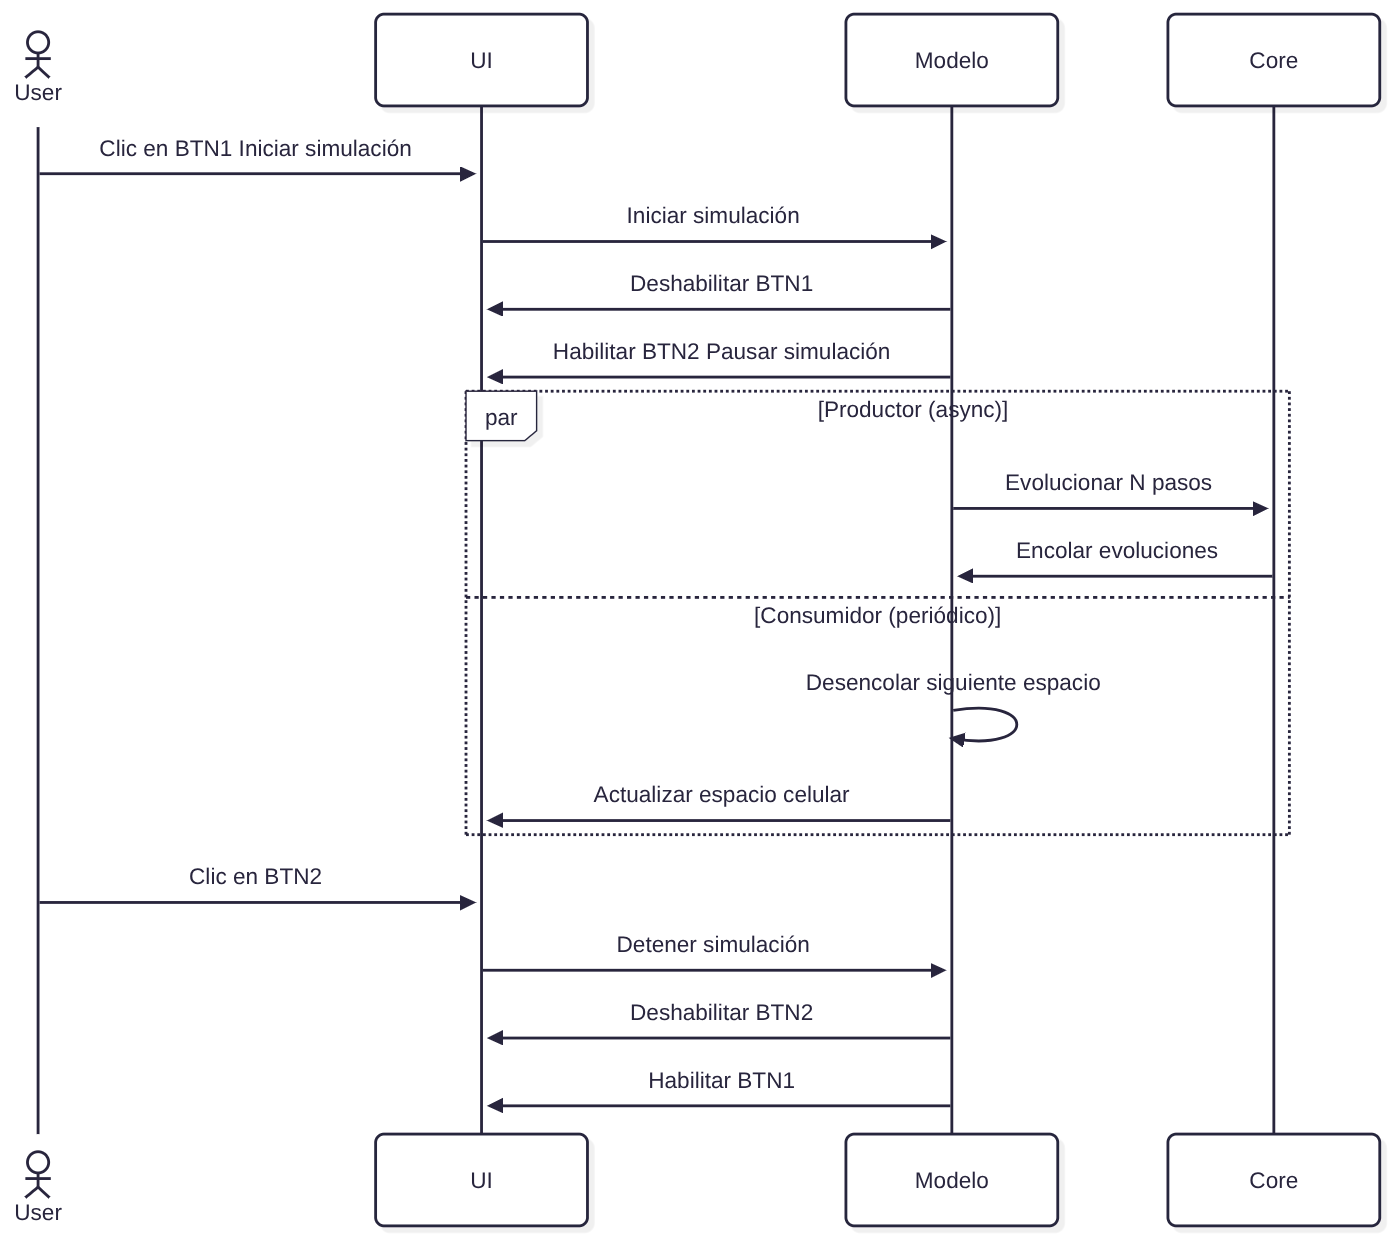
\includegraphics[width=0.95\linewidth]{img/ingenieriaSoftware/sequence_uc01.png}
	\caption{Diagrama de secuencia: UC01 Iniciar simulación.}
	\label{fig:sequence_uc01}
\end{figure}

\begin{figure}[H]
	\centering
	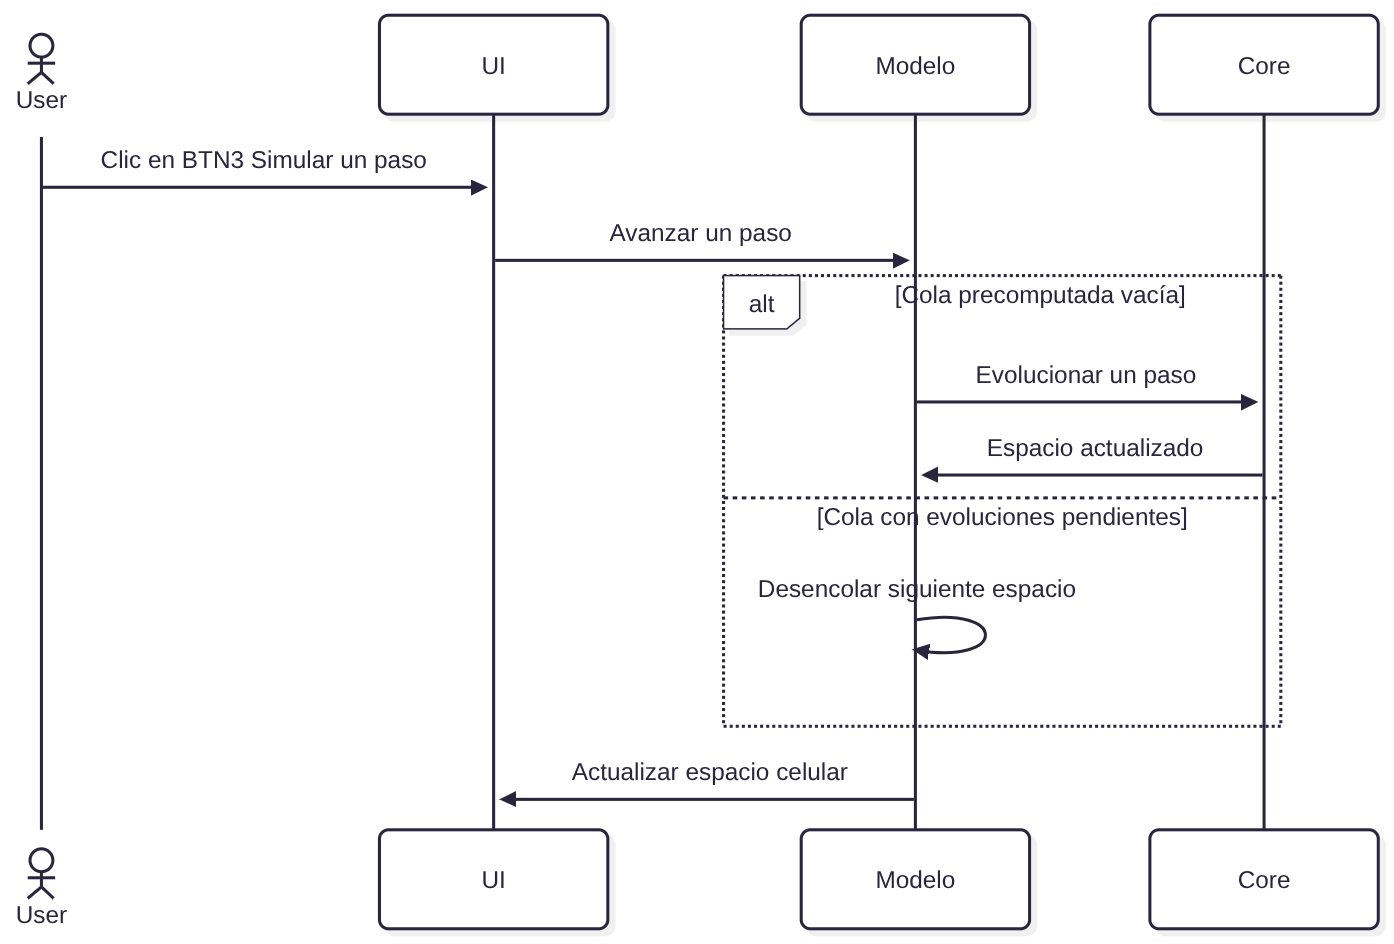
\includegraphics[width=0.95\linewidth]{img/ingenieriaSoftware/sequence_uc04.png}
	\caption{Diagrama de secuencia: UC04 Simular un paso.}
	\label{fig:sequence_uc04}
\end{figure}

\begin{figure}[H]
	\centering
	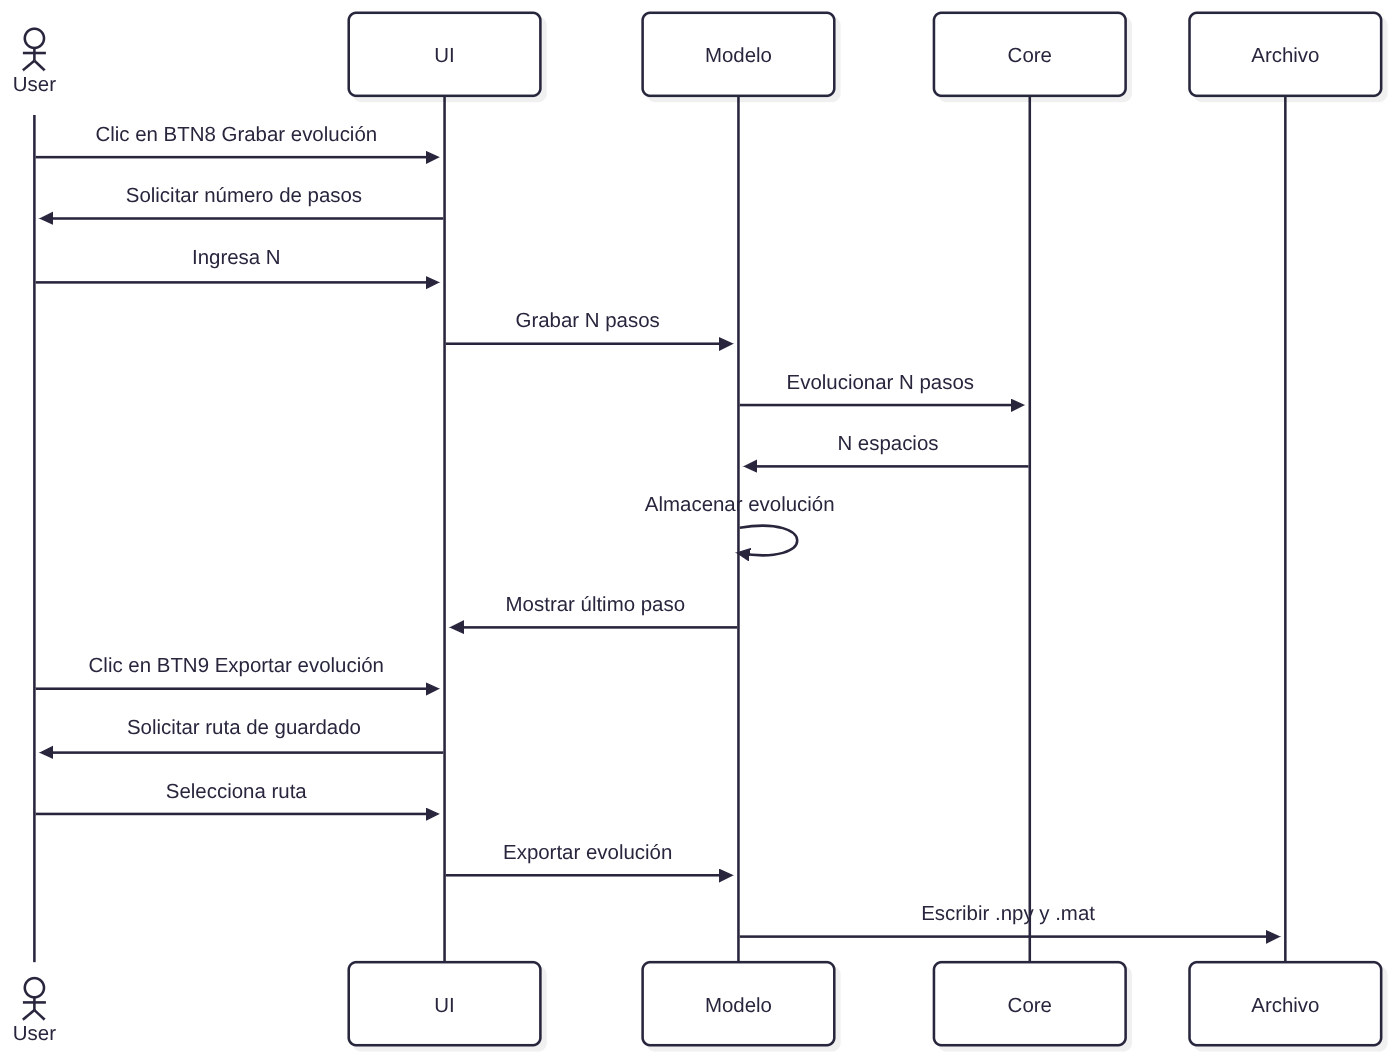
\includegraphics[width=0.95\linewidth]{img/ingenieriaSoftware/sequence_uc10.png}
	\caption{Diagrama de secuencia: UC09 Grabar evolución y UC10 Exportar evolución.}
	\label{fig:sequence_uc10}
\end{figure}

\begin{figure}[H]
	\centering
	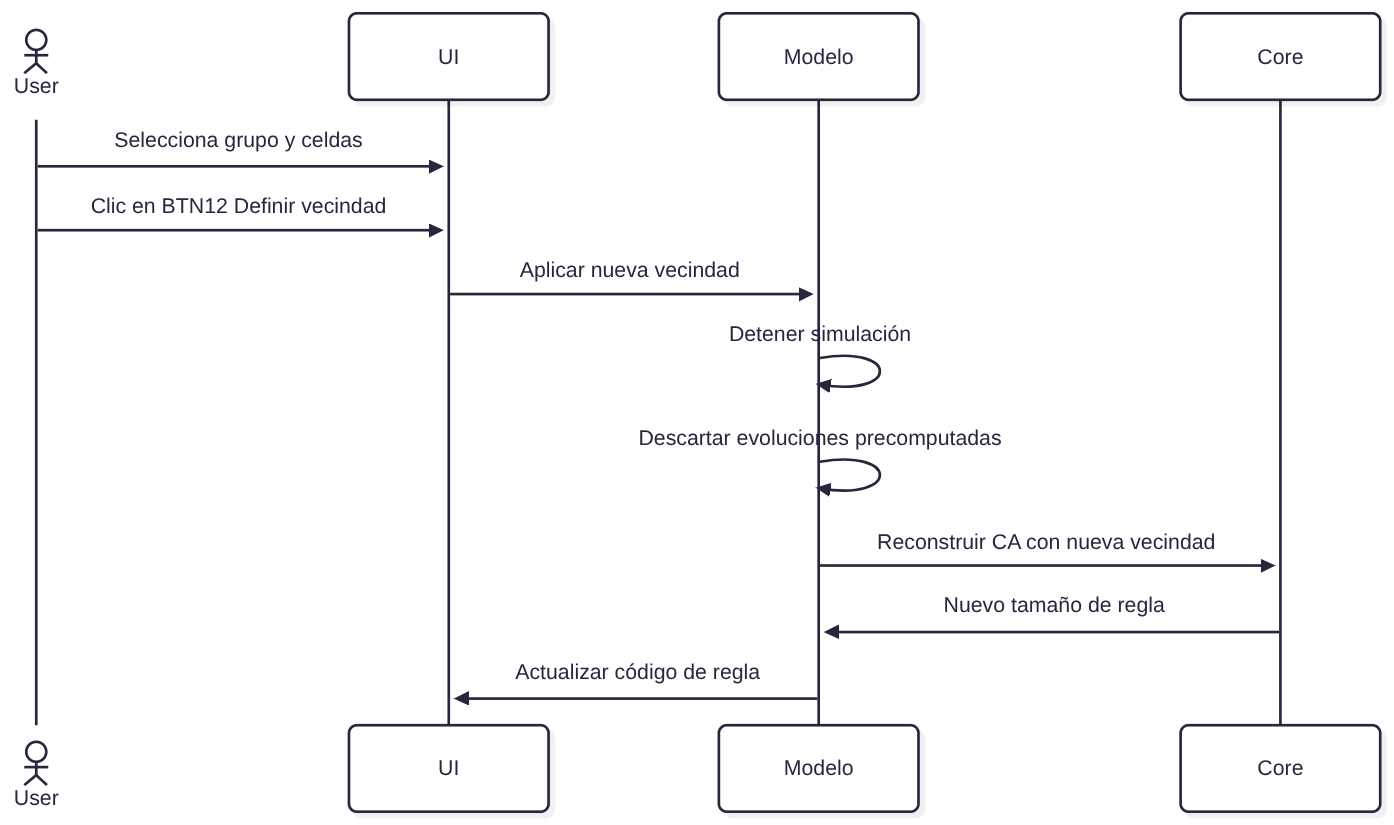
\includegraphics[width=0.95\linewidth]{img/ingenieriaSoftware/sequence_uc13.png}
	\caption{Diagrama de secuencia: UC13 Definir vecindad.}
	\label{fig:sequence_uc13}
\end{figure}

\begin{figure}[H]
	\centering
	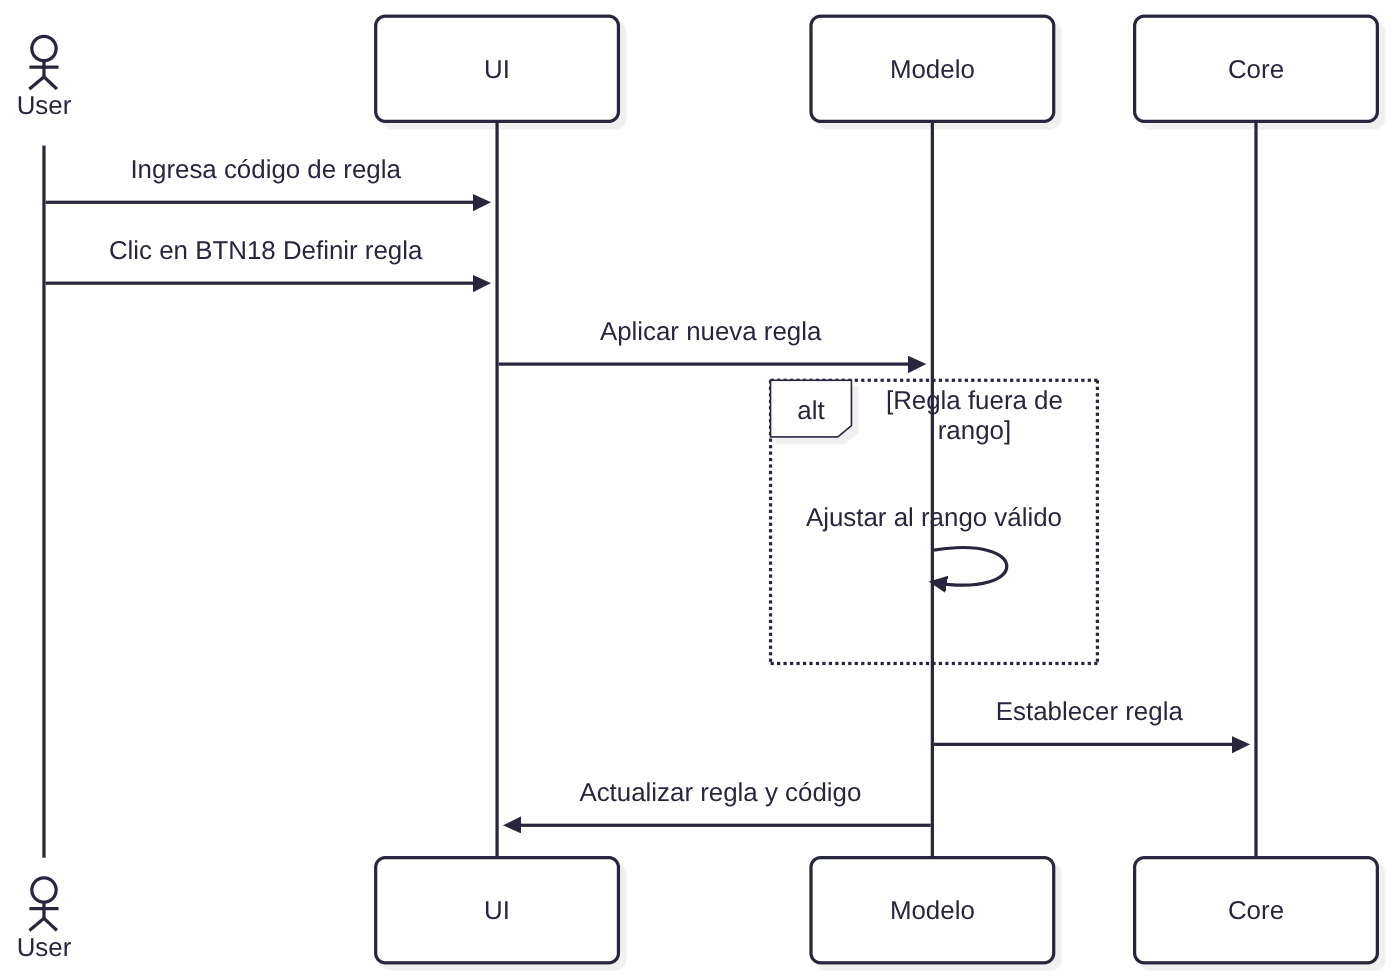
\includegraphics[width=0.95\linewidth]{img/ingenieriaSoftware/sequence_uc16.png}
	\caption{Diagrama de secuencia: UC16 Definir regla de transición.}
	\label{fig:sequence_uc16}
\end{figure}

\begin{figure}[H]
	\centering
	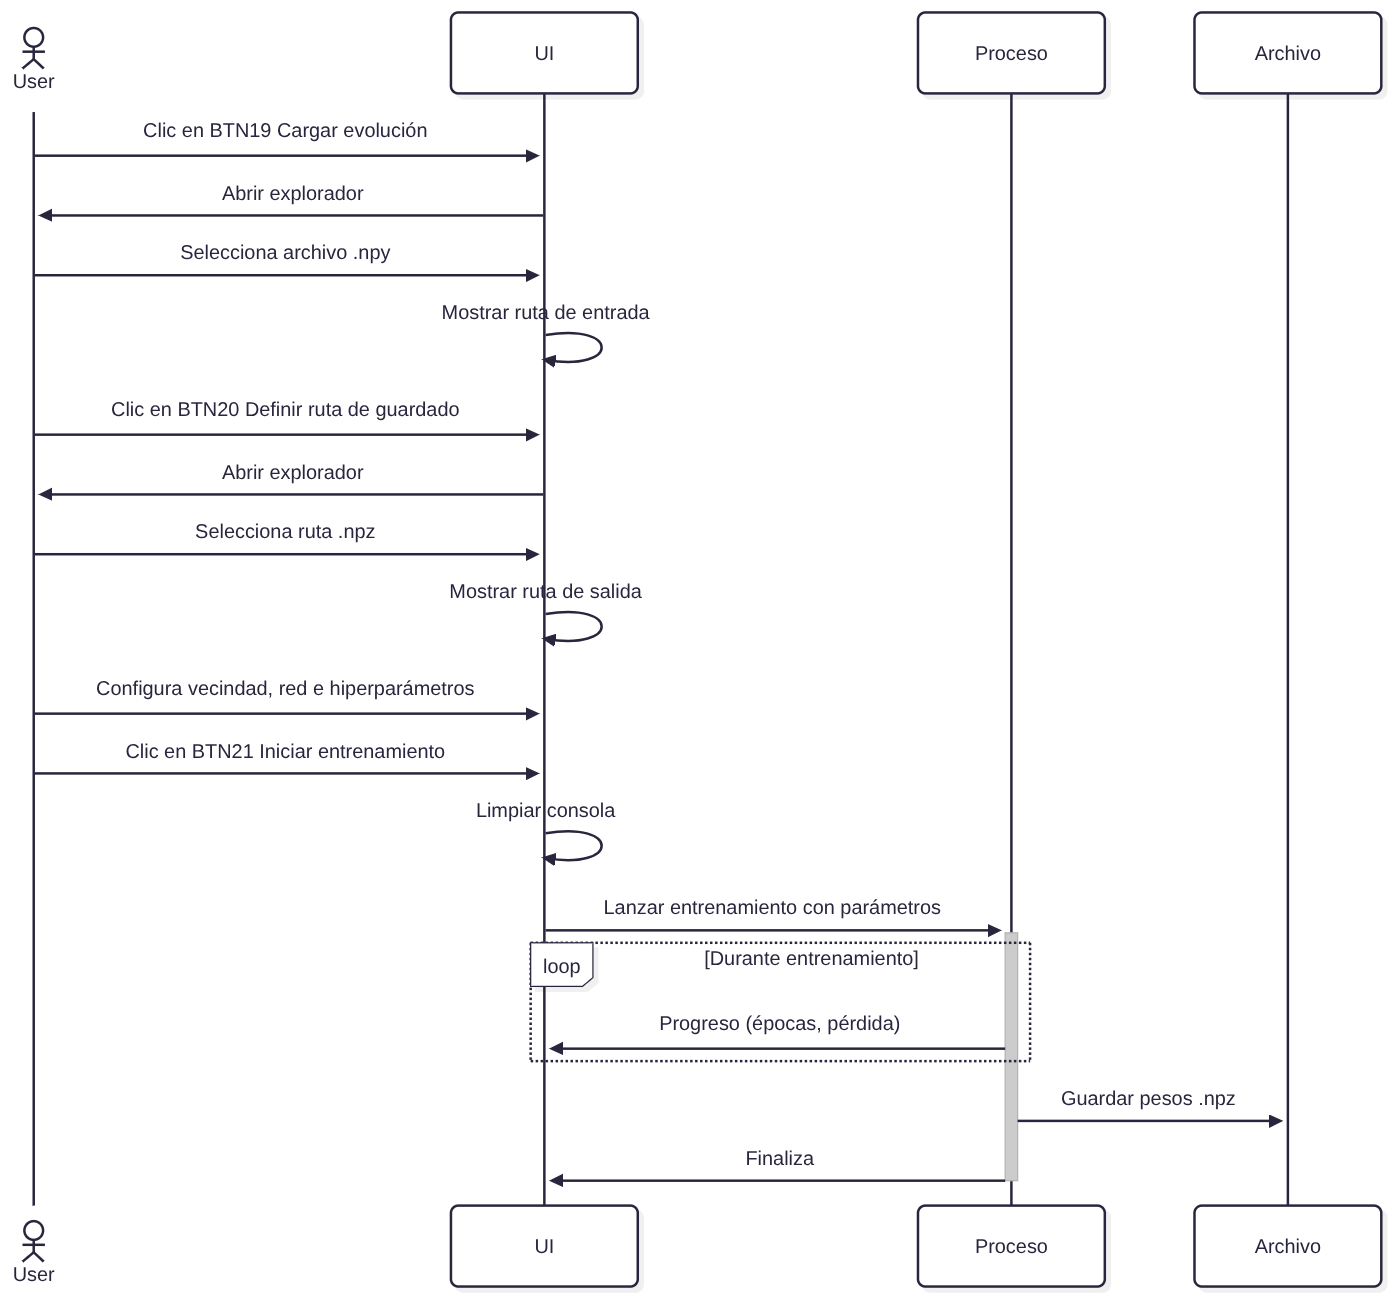
\includegraphics[width=0.95\linewidth]{img/ingenieriaSoftware/sequence_uc19.png}
	\caption{Diagrama de secuencia: UC19 Iniciar entrenamiento.}
	\label{fig:sequence_uc19}
\end{figure}

\begin{comment}
	\begin{figure}[H]
		\centering
		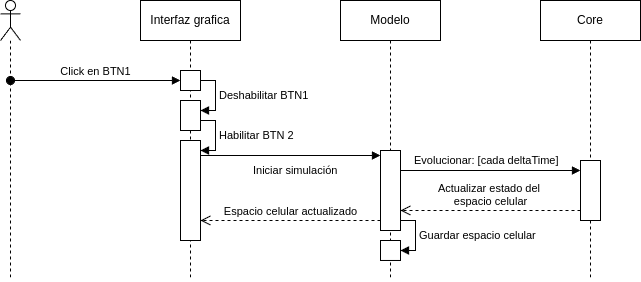
\includegraphics[width=0.9\linewidth]{img/ingenieriaSoftware/UML_SD_UC01.png}
		\caption{Diagrama de secuencia: UC01 Iniciar simulación.}
		\label{fig:UML_SD_UC01}
	\end{figure}
	
	\begin{figure}[H]
		\centering
		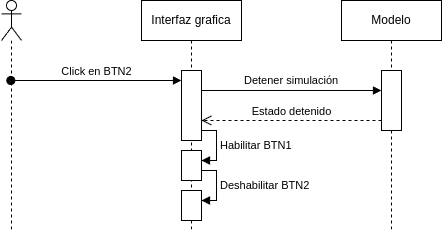
\includegraphics[width=0.7\linewidth]{img/ingenieriaSoftware/UML_SD_UC02.png}
		\caption{Diagrama de secuencia: UC02 Pausar simulación.}
		\label{fig:UML_SD_UC02}
	\end{figure}
	
	\begin{figure}[H]
		\centering
		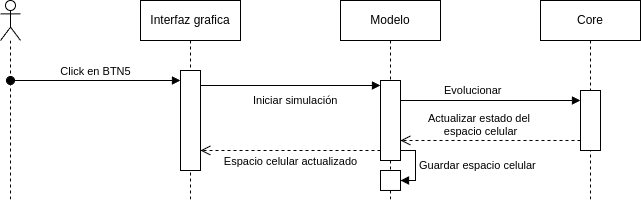
\includegraphics[width=0.9\linewidth]{img/ingenieriaSoftware/UML_SD_UC05.png}
		\caption{Diagrama de secuencia: UC05 Simular un paso.}
		\label{fig:UML_SD_UC05}
	\end{figure}
	
	\begin{figure}[H]
		\centering
		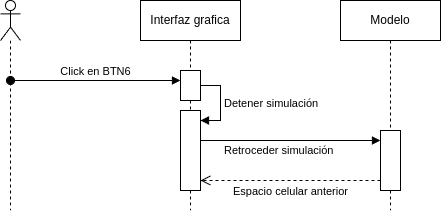
\includegraphics[width=0.7\linewidth]{img/ingenieriaSoftware/UML_SD_UC06.png}
		\caption{Diagrama de secuencia: UC06 Retroceder un paso.}
		\label{fig:UML_SD_UC06}
	\end{figure}
	
	\begin{figure}[H]
		\centering
		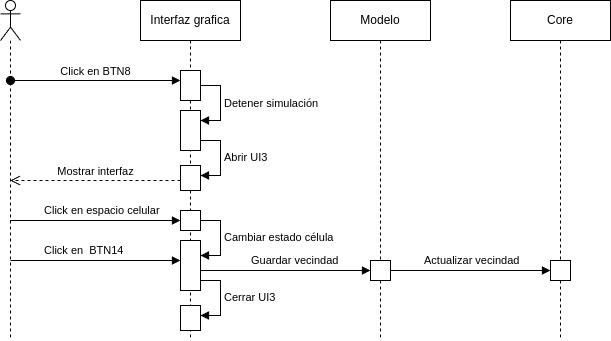
\includegraphics[width=0.9\linewidth]{img/ingenieriaSoftware/UML_SD_UC08.png}
		\caption{Diagrama de secuencia: UC08 Definir vecindad.}
		\label{fig:UML_SD_UC08}
	\end{figure}
	
	\begin{figure}[H]
		\centering
		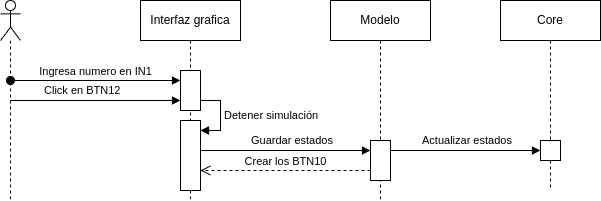
\includegraphics[width=0.9\linewidth]{img/ingenieriaSoftware/UML_SD_UC11.png}
		\caption{Diagrama de secuencia: UC11 Definir numero de estados.}
		\label{fig:UML_SD_UC11}
	\end{figure}
	
	\begin{figure}[H]
		\centering
		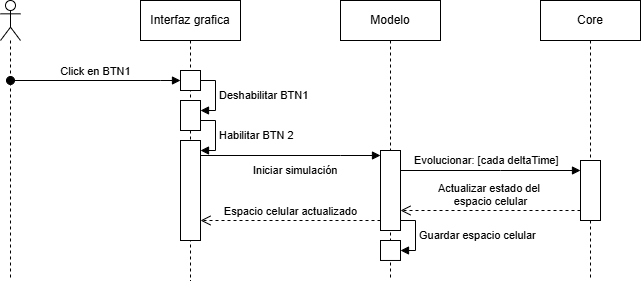
\includegraphics[width=0.9\linewidth]{img/ingenieriaSoftware/UML_SD_UC12.png}
		\caption{Diagrama de secuencia: UC12 Definir función de transición.}
		\label{fig:UML_SD_UC12}
	\end{figure}
\end{comment}



		
	\chapter{Diseño de software}

\section{Arquitectura}

La arquitectura del sistema se basa en el patrón de diseño modelo vista controlador, el cual resulta adecuado para aplicaciones que combinan lógica de negocio, manipulación de datos y una interfaz gráfica interactiva \cite{mvc}. Este patrón favorece la separación de responsabilidades, la mantenibilidad y la extensibilidad del sistema. 

\begin{itemize}
	\item \textbf{Modelo:} Gestiona los datos y la lógica principal del autómata celular, incluyendo la definición de estados, reglas, vecindad y condiciones de frontera.
	\item \textbf{Vista:} Se encarga de la presentación visual de la información y la interacción con el usuario mediante la interfaz gráfica.
	\item \textbf{Controlador:} Actúa como intermediario entre el modelo y la vista, gestionando los eventos de usuario y actualizando el modelo o la interfaz según corresponda.
\end{itemize}

\subsection{Vista}
La vista está implementada en \textit{Python} utilizando el framework \textbf{PyQt5}. Esta capa proporciona la interfaz gráfica principal del simulador, permitiendo visualizar y controlar el espacio celular y entrenar el autómata celular neuronal.

\subsection{Modelo}

El modelo encapsula la lógica del autómata celular. Esta capa está implementada en \textit{C++} y CUDA con el fin de optimizar el rendimiento en las operaciones de actualización de celdas y el procesamiento paralelo. El modelo gestiona la estructura del espacio celular, los estados, la topología de la vecindad, las condiciones de frontera y la regla de transición.

\subsection{Controlador}

El \textbf{controlador} coordina la comunicación entre la vista y el modelo. Implementado en Python, este componente recibe los eventos generados por la interfaz, actualiza el modelo y refleja los resultados en la interfaz gráfica. Además, sincroniza los procesos de simulación y representación visual.

\begin{figure}[H]
	\centering
	\includegraphics[width=.9 \linewidth]{"./img/flowchartDiagram.png"}
	\caption{Diagrama de arquitectura del sistema.}
	\label{fig:flujo}
\end{figure}
	\section{Diagrama de clases}

El diagrama de clases UML sirve para mostrar una vista estática de las clases de un sistema, sus atributos, métodos y relaciones entre objetos. Sirve para proporcionar una información general sobre la aplicación \cite{clase}. 

El diagrama de clases se compone de tres partes: 
\begin{itemize}[nosep, noitemsep]
	\item \textbf{CUDA}: La figura \ref{fig:class_cuda} muestra la definición de las clases del autómata celular y el autómata celular neuronal. 
	\item \textbf{Modelos}: Son los modelos construidos con pybind11 los cuales son manipulados por ``SimulationController'', como se muestra en la figura \ref{fig:class_models}.
	\item \textbf{UI}: Elementos y controladores de la interfaz gráfica en PyQt5. Ver figura \ref{fig:class_ui}.
\end{itemize}

\begin{figure}[H]
	\centering
	\includegraphics[width=.7 \linewidth]{"./img/classDiagram_cuda.png"}
	\caption{Diagrama de clases: Capa CUDA}
	\label{fig:class_cuda}
\end{figure}

\begin{figure}[H]
	\centering
	\includegraphics[width=.95 \linewidth]{"./img/classDiagram_models.png"}
	\caption{Diagrama de clases: Capa de modelos}
	\label{fig:class_models}
\end{figure}

\begin{figure}[H]
	\centering
	\includegraphics[width=.95 \linewidth]{"./img/classDiagram_ui.png"}
	\caption{Diagrama de clases: Capa UI}
	\label{fig:class_ui}
\end{figure}
	\section{Diseño de Datos}

El simulador maneja seis estructuras de datos principales: el espacio celular, la vecindad, la regla de transición, la configuración del autómata celular, la configuración del autómata celular neuronal y el historial de las evoluciones. A continuación se definen estas variables y cómo evolucionan en las diferentes capas del sistema.

La información dentro de CUDA, también llamado \textit{device}, no puede almacenar arreglos multidimensionales. Por esta razón, almacena matrices y tensores como un único arreglo unidimensional continuo y se accede a los indices de forma manual. Resulta necesario hacer un mapeo entre Python, también \textit{host}, con el \textit{device}.

\subsection{Espacio Celular}

Se define como una matriz bidimensional de dimensiones $H \times W$ con valores enteros de 8~bits, permitiendo representar hasta 256 estados distintos por celda.

\begin{itemize}
	\item \textbf{Host}: Implementado como un \texttt{numpy.ndarray} de \textit{shape} $(H, W)$ y \texttt{dtype=uint8}. Para maximizar el rendimiento, este arreglo se comparte mediante punteros, sin realizar copias, entre el \textit{widget} de renderizado, el controlador de simulación y el \textit{wrapper} de CUDA.
	
	\item \textbf{Device}: Utiliza dos búferes (\texttt{A\_d} y \texttt{B\_d}) de tipo \texttt{uint8\_t*} en la memoria global. Tienen un esquema de \textit{ping-pong buffering}, donde tras cada iteración del kernel, se intercambian los punteros de lectura y escritura, eliminando la necesidad de copiar datos entre pasos de evolución.
	
	\item \textbf{Sincronización perezosa}: El \textit{host} no se sincroniza tras cada paso del kernel. Una bandera \texttt{host\_dirty} indica si el búfer del \textit{host} está desactualizado respecto al \textit{device}; la copia \textit{device-to-host} se ejecuta únicamente cuando se invoca una operación de lectura (\texttt{getSpace}, \texttt{getCell}) o al exportar.
\end{itemize}

\subsection{Vecindad}

La vecindad define el conjunto de celdas que influyen en la transición de una celda objetivo. Se modela bajo un esquema semitotalístico organizado en grupos de desplazamientos relativos.

\begin{itemize}
	\item \textbf{Host}: Una estructura \texttt{list[list[list[int]]]} donde el nivel externo enumera los grupos, el intermedio las posiciones relativas, y el interno los componentes $[dx, dy]$ del desplazamiento.
	
	\item \textbf{Device}: La vecindad se define mediante dos arreglos: (1) \texttt{neighbourhood[]} que contiene los vectores de desplazamiento concatenados y (2) \texttt{group\_sizes[]} que almacena los tamaños de los grupos. 
	
	\item \textbf{Cotas técnicas}: Se establece un límite de $n_{\text{size}} \leq 64$ desplazamientos totales y $n_{\text{groups}} \leq 64$ grupos para cumplir con las restricciones de la memoria constante.
\end{itemize}

\subsection{Regla de Transición (CA Clásico)}

La regla es de naturaleza semitotalística: el nuevo estado depende del conteo de estados dentro de cada grupo de la vecindad. El tamaño total $r_{\text{size}}$ se determina por el producto de las combinaciones posibles de cada grupo:
\[
r_{\text{size}} = \prod_{g \in \text{grupos}} \big((\text{states}-1)\cdot |g| + 1\big)
\]
donde $|g|$ es la cardinalidad del grupo y \texttt{states} el número de estados permitidos.

El acceso a la regla se realiza mediante una suma posicional de las contribuciones de cada grupo de vecindad, calculando un índice lineal único para cada configuración de conteos.

\begin{itemize}
	\item \textbf{Host}: \texttt{numpy.ndarray} de \texttt{uint8}, tamaño $r_{\text{size}}$.
	
	\item \textbf{Device}: Debido a que $r_{\text{size}}$ puede alcanzar hasta $16,777,216$ entradas, la tabla reside en la memoria global del dispositivo (\texttt{rule\_d}).
\end{itemize}

\subsection{Configuración del Autómata Celular (CA)}

Esta estructura encapsula los parámetros estáticos que definen el comportamiento de un autómata clásico:

\begin{center}
	\begin{tabular}{c|c | p{0.42\linewidth}}
		\hline
		\textbf{Campo} & \textbf{Tipo} & \textbf{Descripción} \\
		\hline 
		\texttt{dimensions} & \texttt{(int, int)} & Dimensiones $H \times W$ del espacio. \\ \hline 
		\texttt{states} & \texttt{uint8} & Estados permitidos (1--256). \\ \hline 
		\texttt{neighbourhood} & \texttt{list[list[list[int]]]} & Definición de grupos de vecindad. \\ \hline 
		\texttt{rule} & \texttt{uint8[]} & Tabla indexada de la sección 3.3. \\ \hline 
		\texttt{boundary\_mode} & \texttt{enum} & Modos: \texttt{OPEN}, \texttt{PERIODIC}, \texttt{REFLECTIVE}, \texttt{REFLEXIVE}. \\ \hline 
		\texttt{colors} & \texttt{list[QColor]} & Mapeo de estados a colores para el renderizado. \\
	\end{tabular}
\end{center}

\subsection{Configuración del Autómata Celular Neuronal (NCA)}

El modelo neuronal sustituye la tabla de reglas por un Perceptrón Multicapa (MLP) que procesa la información de la vecindad.

\begin{itemize}
	\item \textbf{Topología del MLP}: Se define mediante \texttt{layer\_in} (entradas según vecindad), \texttt{layer\_out} (neuronas de salida), \texttt{hidden\_layers[]} (arquitectura oculta) y \texttt{activations[]} (códigos: \texttt{0=ReLU}, \texttt{1=Sigmoid}, \texttt{2=Tanh}, \texttt{3=Linear}).
	
	\item \textbf{Pesos y Sesgos}: Se organizan en un arreglo plano de tipo \texttt{float} con un vector de desplazamientos (\textit{offsets}). Esta estructura lineal favorece el acceso coalescente en la GPU y minimiza la fragmentación de memoria.
	
	\item \textbf{Formato de Intercambio}: La persistencia se realiza en archivos \texttt{.npz} (NumPy) que contienen los tensores de pesos, sesgos y los metadatos de la topología, permitiendo una carga directa en la interfaz gráfica.
\end{itemize}

\subsection{Historial de Evoluciones}

El historial gestiona el estado temporal de la simulación mediante búferes en memoria y persistencia en disco.

\begin{itemize}
	\item \textbf{Gestión de Memoria}: 
	\begin{itemize}
		\item \texttt{past\_record}: Lista de instantáneas \texttt{ndarray} para permitir el retroceso cronológico.
		\item \texttt{future\_record}: Un \texttt{collections.deque} que almacena estados precomputados asíncronamente por un \texttt{PrefetchWorker}.
	\end{itemize}
	
	\item \textbf{Grabación de Alto Rendimiento}: Se utiliza memoria \textit{pinned} (fija) reservada con \texttt{cudaHostAlloc}. Esto permite que el flujo de datos dispositivo--anfitrión sea asíncrono y no se vea penalizado por la paginación del sistema operativo.
	
	\item \textbf{Formatos de Salida}: Los datos se exportan simultáneamente en \texttt{.npy} (para re-entrenamiento en Python) y \texttt{.mat} (para análisis y validación en Wolfram Mathematica).
\end{itemize}
	\section{Diseño de algoritmos}

Dentro del simulador existen seis algoritmos no triviales que determinan el correcto funcionamiento de todos los módulos. Estos algoritmos son: la indexación de la regla semitotalística, el paso de evolución del autómata celular clásico, el manejo de las condiciones de frontera, el \textit{forward pass} del autómata celular neuronal, el entrenamiento del modelo neuronal y el \textit{prefetch} asíncrono. En esta sección se presentan los pseudocódigos de dichos algoritmos junto con sus decisiones de diseño.

Para homogeneizar los algoritmos, todos se rigen bajo las siguientes convenciones:
\begin{itemize}
    \item Los arreglos se indexan desde cero.
    \item \texttt{H} y \texttt{W} son alto y ancho del espacio celular.
    \item El acceso a una posición del espacio celular en su forma unidimensional se realiza mediante el siguiente cálculo: \texttt{A[y\,$\cdot$\,W + x]}.
    \item \texttt{states} es el número de estados permitidos por célula.
    \item \texttt{n\_groups} y \texttt{group\_sizes[]} describen la partición en grupos de la vecindad.
\end{itemize}

\subsection{Indexación de la regla semitotalística}

La tabla de regla \texttt{rule[]} contiene una entrada por cada combinación posible de conteos por grupo. Para acceder a la entrada correcta durante la evaluación de una célula, se requiere convertir el vector de conteos en un índice lineal único. Este algoritmo se invoca $H \times W$ veces por cada paso evolutivo.

Cada grupo $g$ aporta una contribución igual a la suma de los estados de las células que lo integran. Esa suma puede tomar valores en $\{0, 1, \dots, (\text{states}-1)\cdot|g|\}$, es decir, $((\text{states}-1)\cdot|g| + 1)$ valores distintos. El índice global se construye en base mixta posicional, multiplicando cada contribución por el producto acumulado de los tamaños de los grupos previos.

\begin{breakablealgorithm}
\caption{IndiceRegla: vector de conteos $\to$ índice lineal}
\label{alg:indice}
\begin{algorithmic}[1]
\Require \texttt{sums[n\_groups]}, \texttt{group\_sizes[n\_groups]}, \texttt{states}
\Ensure \texttt{idx} $\in [0, r_{\text{size}})$
\State $\texttt{idx} \gets 0$
\State $\texttt{mult} \gets 1$
\For{$g \gets 0$ \textbf{to} $\texttt{n\_groups} - 1$}
    \State $\texttt{idx} \gets \texttt{idx} + \texttt{sums}[g] \cdot \texttt{mult}$
    \State $\texttt{mult} \gets \texttt{mult} \cdot ((\texttt{states} - 1) \cdot \texttt{group\_sizes}[g] + 1)$
\EndFor
\State \Return \texttt{idx}
\end{algorithmic}
\end{breakablealgorithm}

\textbf{Complejidad}: $\mathcal{O}(\texttt{n\_groups})$ por célula. 

En el juego de la vida existen dos grupos: los 8 vecinos de Moore y la célula central, y dos estados (vivo/muerto). El tamaño de la tabla resulta $r_{\text{size}} = \bigl((2-1)\cdot 8  + 1\bigr)\cdot\bigl((2-1)\cdot 1 + 1\bigr) = 9 \cdot 2 = 18$ entradas, indexadas por el conteo de vecinos vivos, lo que corresponde a la formulación clásica B3/S23.

\subsection{Paso de evolución del autómata celular clásico}

En cada paso evolutivo el \textit{kernel} CUDA gestiona los hilos responsables de calcular el nuevo estado de todas las células. La cuadrícula se mapea a una topología bidimensional de bloques: cada bloque cubre $16 \times 16$ células, y los bloques se organizan en un \textit{grid} de tamaño $\lceil W/16 \rceil \times \lceil H/16 \rceil$.

Para cada célula, el hilo recorre la vecindad agrupada, acumula la suma de estados por grupo, calcula el índice de la regla y escribe el resultado en el búfer destino. Tras el \textit{kernel}, los punteros \texttt{A\_d} y \texttt{B\_d} se intercambian (\textit{ping-pong}), evitando copias entre pasos.

\begin{breakablealgorithm}
\caption{stepKernel$\langle$\texttt{BoundaryMode}$\rangle$: un paso de evolución del autómata celular}
\label{alg:step-ca}
\begin{algorithmic}[1]
\Require búfer origen \texttt{A[H$\cdot$W]}, búfer destino \texttt{B[H$\cdot$W]}, \texttt{neighbourhood[n\_size]}, \texttt{group\_sizes[n\_groups]}, \texttt{rule[r\_size]}
\State $(x, y) \gets$ coordenadas del hilo en el \textit{grid}
\If{$x \geq W$ \textbf{or} $y \geq H$} \State \Return \EndIf
\State $\texttt{offset} \gets 0$;\quad $\texttt{idx} \gets 0$;\quad $\texttt{mult} \gets 1$
\For{$g \gets 0$ \textbf{to} $\texttt{n\_groups} - 1$}
    \State $\texttt{sum} \gets 0$
    \For{$i \gets 0$ \textbf{to} $\texttt{group\_sizes}[g] - 1$}
        \State $(dx, dy) \gets \texttt{neighbourhood}[\texttt{offset} + i]$
        \State $(x', y', \texttt{valid}) \gets \textsc{ApplyBoundary}\langle\texttt{BoundaryMode}\rangle(x + dx, y + dy, W, H)$
        \If{\texttt{valid}}
            \State $\texttt{sum} \gets \texttt{sum} + \texttt{A}[y' \cdot W + x']$
        \EndIf
    \EndFor
    \State $\texttt{idx} \gets \texttt{idx} + \texttt{sum} \cdot \texttt{mult}$
    \State $\texttt{mult} \gets \texttt{mult} \cdot ((\texttt{states} - 1) \cdot \texttt{group\_sizes}[g] + 1)$
    \State $\texttt{offset} \gets \texttt{offset} + \texttt{group\_sizes}[g]$
\EndFor
\State $\texttt{B}[y \cdot W + x] \gets \texttt{rule}[\texttt{idx}]$
\end{algorithmic}
\end{breakablealgorithm}

El parámetro \texttt{BoundaryMode} es un argumento de plantilla, no un parámetro en tiempo de ejecución. El compilador genera cuatro versiones del \textit{kernel} (una por modo de frontera) y el \texttt{if constexpr} dentro de \textsc{ApplyBoundary} elimina toda ramificación condicional en la GPU, lo que evita la divergencia de \textit{warps} en células cercanas al borde.

\textbf{Complejidad}: $\mathcal{O}(\texttt{n\_size})$ por célula, $\mathcal{O}(H \cdot W \cdot \texttt{n\_size})$ por paso.

\subsection{Manejo de condiciones de frontera}

Las cuatro condiciones de frontera modifican la coordenada de un vecino que cae fuera del dominio antes de leerlo. Cada modo se implementa como una función separada, pero con la misma firma.

\begin{breakablealgorithm}
\caption{ApplyBoundary: cuatro variantes especializadas en compilación}
\label{alg:frontera}
\footnotesize
\begin{algorithmic}[1]
\Function{ApplyBoundary}{OPEN, $x, y, W, H$}
    \State \textbf{if} $x < 0$ \textbf{or} $x \geq W$ \textbf{or} $y < 0$ \textbf{or} $y \geq H$ \textbf{then return} $(0, 0, \texttt{false})$
    \State \Return $(x, y, \texttt{true})$
\EndFunction
\Statex
\Function{ApplyBoundary}{PERIODIC, $x, y, W, H$}
    \State \Return $((x \bmod W + W) \bmod W,\; (y \bmod H + H) \bmod H,\; \texttt{true})$
\EndFunction
\Statex
\Function{ApplyBoundary}{REFLECTIVE, $x, y, W, H$}
    \Comment{La frontera actúa como un espejo}
    \State \textbf{if} $x < 0$ \textbf{then} $x \gets -x - 1$;\quad \textbf{if} $x \geq W$ \textbf{then} $x \gets 2W - x - 1$
    \State \textbf{if} $y < 0$ \textbf{then} $y \gets -y - 1$;\quad \textbf{if} $y \geq H$ \textbf{then} $y \gets 2H - y - 1$
    \State \Return $(x, y, \texttt{true})$
\EndFunction
\Statex
\Function{ApplyBoundary}{REFLEXIVE, $x, y, W, H$}
    \Comment{El borde se trata como una célula real}
    \State \textbf{if} $x < 0$ \textbf{then} $x \gets -x$;\quad \textbf{if} $x \geq W$ \textbf{then} $x \gets 2W - x - 2$
    \State \textbf{if} $y < 0$ \textbf{then} $y \gets -y$;\quad \textbf{if} $y \geq H$ \textbf{then} $y \gets 2H - y - 2$
    \State \Return $(x, y, \texttt{true})$
\EndFunction
\end{algorithmic}
\end{breakablealgorithm}

\textbf{Complejidad}: $\mathcal{O}(\texttt{1})$.

\subsection{\textit{Forward pass} del autómata celular neuronal}

El autómata celular neuronal, a diferencia del clásico, utiliza un perceptrón multicapa que se evalúa de forma independiente sobre cada célula. El \textit{kernel} CUDA mantiene la misma estructura que el autómata celular, ejecutando un hilo por cada célula. Sin embargo, en lugar de un acceso a la tabla, se ejecuta una secuencia de productos matriz-vector con activaciones intercaladas.

Los pesos y sesgos de las capas residen en dos arreglos planos \texttt{weights[]} y \texttt{biases[]}, con los vectores \texttt{w\_offsets[]} y \texttt{b\_offsets[]}, que apuntan al inicio de cada matriz $W_\ell$ y de cada vector de sesgos $b_\ell$. 

\begin{breakablealgorithm}
\caption{ncaKernel: \textit{forward pass} del MLP por célula}
\label{alg:nca-fwd}
\begin{algorithmic}[1]
\Require \texttt{A}, \texttt{B}, \texttt{neighbourhood[n\_size]}, \texttt{weights[]}, \texttt{biases[]}, \texttt{w\_offsets[]}, \texttt{b\_offsets[]}, \texttt{layer\_sizes[n\_layers+1]}, \texttt{activations[n\_layers]}
\State $(x, y) \gets$ coordenadas del hilo
\If{$x \geq W$ \textbf{or} $y \geq H$} \State \Return \EndIf
\State $\texttt{input}[\texttt{n\_size}] \gets$ vector de tamaño $\texttt{n\_size}$
\For{$i \gets 0$ \textbf{to} $\texttt{n\_size} - 1$}
    \State $(dx, dy) \gets \texttt{neighbourhood}[i]$
    \State $(x', y', \_) \gets \textsc{ApplyBoundary}(x + dx, y + dy, W, H)$
    \State $\texttt{input}[i] \gets \texttt{A}[y' \cdot W + x']$
\EndFor
\State $\texttt{current} \gets \texttt{input}$
\For{$\ell \gets 0$ \textbf{to} $\texttt{n\_layers} - 1$}
    \State $W_\ell \gets \texttt{weights} + \texttt{w\_offsets}[\ell]$
    \State $b_\ell \gets \texttt{biases} + \texttt{b\_offsets}[\ell]$
    \State $n_{\text{in}} \gets \texttt{layer\_sizes}[\ell]$;\quad $n_{\text{out}} \gets \texttt{layer\_sizes}[\ell+1]$
    \For{$j \gets 0$ \textbf{to} $n_{\text{out}} - 1$}
        \State $s \gets b_\ell[j]$
        \For{$k \gets 0$ \textbf{to} $n_{\text{in}} - 1$}
            \State $s \gets s + W_\ell[j \cdot n_{\text{in}} + k] \cdot \texttt{current}[k]$
        \EndFor
        \State $\texttt{next}[j] \gets \textsc{Activar}(s,\; \texttt{activations}[\ell])$
    \EndFor
    \State $\texttt{current} \gets \texttt{next}$
\EndFor
\State $\texttt{B}[y \cdot W + x] \gets \texttt{current}[0]$
\end{algorithmic}
\end{breakablealgorithm}
Se evita el uso de \texttt{std::function} u otros punteros a función, ya que no son compatibles con \textit{kernels} CUDA.

\textbf{Complejidad}: $\displaystyle \mathcal{O}\left(\texttt{n\_size} + \sum_{\ell = 0}^{L - 1}(n_\ell \cdot n_{\ell+1})\right)$ por célula. 

\subsection{Entrenamiento del autómata celular neuronal}

El entrenamiento parte de una evolución registrada en formato $(T, H, W)$ y produce los pesos del perceptrón multicapa que mejor reproducen la transición observada. El procedimiento se ejecuta en PyTorch fuera del módulo CUDA, en CPU o GPU según disponibilidad.

A diferencia del aprendizaje supervisado tradicional sobre imágenes, aquí cada par de entrenamiento corresponde a una célula individual: la entrada es el vector de estados en su vecindad en el instante $t$, y el objetivo es el estado de la misma célula en el instante $t+1$.

\begin{breakablealgorithm}
\caption{EntrenarNCA: ajuste del MLP a partir de una evolución registrada}
\label{alg:entrenar}
\begin{algorithmic}[1]
\Require \texttt{evolucion}$\in \mathbb{R}^{T \times H \times W}$, \texttt{vecindad}, \texttt{arq[]} (tamaños de capa), \texttt{act[]} (activaciones), \texttt{lr}, \texttt{epochs\_max}, \texttt{batch}, \texttt{loss\_target}
\Ensure pesos y sesgos del MLP
\Statex
\State $X \gets [\ ]$;\quad $Y \gets [\ ]$ \Comment{Extracción de pares (vecindad, objetivo)}
\For{$t \gets 0$ \textbf{to} $T - 2$}
    \For{$y \gets 0$ \textbf{to} $H - 1$}
        \For{$x \gets 0$ \textbf{to} $W - 1$}
            \State $v \gets [\ ]$
            \ForAll{$(dx, dy) \in \texttt{vecindad}$}
                \State $v.\textsc{append}(\texttt{evolucion}[t,\; (y+dy) \bmod H,\; (x+dx) \bmod W])$
            \EndFor
            \State $X.\textsc{append}(v)$
            \State $Y.\textsc{append}(\texttt{evolucion}[t+1, y, x])$
        \EndFor
    \EndFor
\EndFor
\Statex
\State $\texttt{modelo} \gets \textsc{ConstruirMLP}(\texttt{arq}, \texttt{act})$
\State $\texttt{optim} \gets \textsc{Adam}(\texttt{modelo.parametros}, \texttt{lr})$
\State $\texttt{criterio} \gets$ \textsc{BCE} si \texttt{out\_size} $= 1$; \textsc{EntropíaCruzada} en otro caso
\Statex
\For{$e \gets 0$ \textbf{to} $\texttt{epochs\_max} - 1$}
    \State $L_{\text{acum}} \gets 0$
    \ForAll{\texttt{(X\_b, Y\_b)} en lotes de tamaño \texttt{batch}}
        \State $\hat{Y} \gets \texttt{modelo}(\texttt{X\_b})$
        \State $L \gets \texttt{criterio}(\hat{Y}, \texttt{Y\_b})$
        \State $\texttt{optim.zero\_grad}()$
        \State $L.\texttt{backward}()$
        \State $\texttt{optim.step}()$
        \State $L_{\text{acum}} \gets L_{\text{acum}} + L$
    \EndFor
    \State $L_{\text{época}} \gets L_{\text{acum}} / n_{\text{lotes}}$
    \If{$L_{\text{época}} < \texttt{loss\_target}$} \State \textbf{break} \EndIf
    \State ajustar \texttt{lr} según \texttt{lr\_schedule}
\EndFor
\State \Return pesos y sesgos del \texttt{modelo}
\end{algorithmic}
\end{breakablealgorithm}

Además del límite \texttt{epochs\_max}, se detiene el entrenamiento si la pérdida promedio por lote de la época cae por debajo de \texttt{loss\_target}. Al final de cada época, la tasa de aprendizaje se ajusta según \texttt{lr\_schedule}. 

\textbf{Complejidad}: La primera fase es $\mathcal{O}(T \cdot H \cdot W \cdot \texttt{n\_size})$. La segunda fase es $\mathcal{O}(E \cdot T \cdot H \cdot W \cdot P)$, donde $E$ es el número de épocas y $P$ representa la cantidad total de parámetros del perceptrón multicapa ($\sum_\ell n_\ell \cdot n_{\ell+1}$).

\subsection{\textit{Prefetch} asíncrono con invalidación por generación}

La interfaz gráfica debe sostener una reproducción visualmente fluida sin bloquear el hilo principal de Qt, incluso cuando el cómputo de un paso es computacionalmente complejo (cuadrículas grandes o autómatas celulares neuronales profundos). Para ello, un \textit{worker} en un hilo del \texttt{QThreadPool} precomputa hasta \texttt{PREFETCH\_SIZE} \textit{frames} y los entrega al \texttt{future\_record} del controlador.

Si el usuario cambia la regla, la vecindad o el estado mientras el \textit{worker} está en ejecución, los \textit{frames} precomputados ya no corresponden a la configuración activa y deben descartarse. La solución es un contador entero \texttt{\_generation} que el controlador incrementa ante cualquier cambio; el \textit{worker} captura su valor al lanzarse y verifica que coincida antes de publicar resultados.

\begin{breakablealgorithm}
\caption{PrefetchWorker.run: producción asíncrona de \textit{frames}}
\label{alg:prefetch}
\begin{algorithmic}[1]
\Require \texttt{automata}, \texttt{gen} (generación capturada al instanciar), \texttt{controller}, $N = \texttt{PREFETCH\_SIZE}$
\State $\texttt{frames} \gets [\ ]$
\For{$i \gets 0$ \textbf{to} $N - 1$}
    \If{$\texttt{controller.generation} \neq \texttt{gen}$}
        \State \Return \Comment{Configuración cambió; descartar trabajo}
    \EndIf
    \State $\texttt{automata.step}()$
    \State $\texttt{frames.append}(\texttt{automata.getSpace}().\texttt{copy}())$
\EndFor
\Statex
\State \textit{// Publicar de regreso al hilo de Qt vía señal}
\If{$\texttt{controller.generation} = \texttt{gen}$}
    \State $\texttt{controller.future\_record.extend}(\texttt{frames})$
\Else
    \State descartar \texttt{frames}
\EndIf
\end{algorithmic}
\end{breakablealgorithm}

La comprobación dentro del bucle permite abortar tempranamente y liberar el hilo del \textit{pool}; la comprobación final antes de publicar evita entregar \textit{frames} obsoletos si la generación cambia justo después del último \texttt{step()}, pero antes de la respuesta.

Cuando el usuario retrocede, los \textit{frames} se consumen desde \texttt{past\_record}; cuando avanza más allá de lo registrado, se consumen desde \texttt{future\_record}. Si este último se vacía, se dispara un nuevo \texttt{PrefetchWorker} con la generación actual.

\textbf{Complejidad}: $\mathcal{O}(N\cdot H\cdot W\cdot c)$, donde $N=\texttt{PREFETCH\_SIZE}$ y $c$ es el costo por célula del paso evolutivo subyacente ($\texttt{n\_size}$ para CA, $\texttt{n\_size}+\sum_\ell n_\ell  n_{\ell+1}$ para NCA).

	\section{Interfaces de usuario}

A continuación se muestran las interfaces desarrolladas en PyQt5. Se busca mantener una estructura intuitiva y modular que facilite la configuración, ejecución y visualización de los autómatas celulares.

\begin{itemize}
	\item \textbf{Pestaña de simulación}

	La pestaña de simulación permite configurar y controlar la evolución de los autómatas celulares, como se observa en la figura \ref{fig:ui_main}. Se divide en tres secciones: 
	
	\begin{figure}[H]
		\centering
		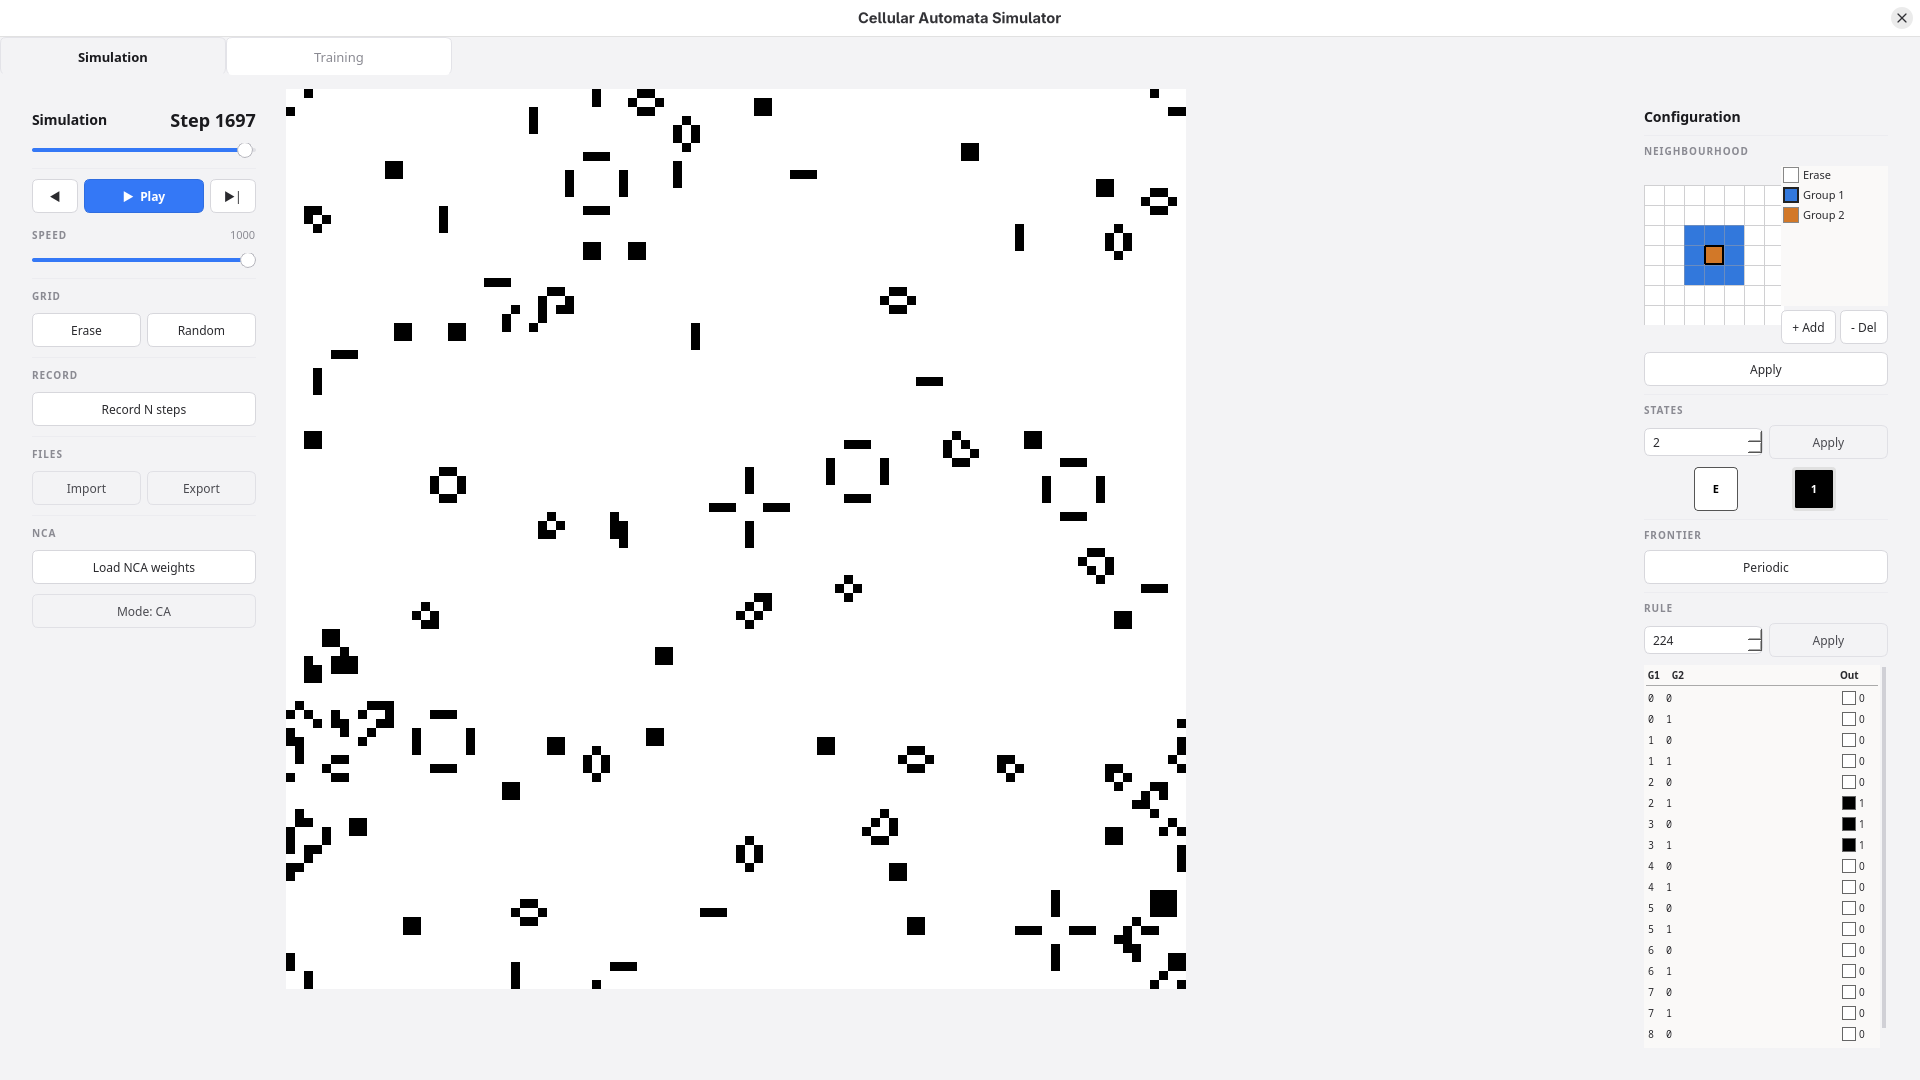
\includegraphics[width=0.9\linewidth]{img/disenoSoftware/ui_main.png}
		\caption{Interfaz de usuario. Pestaña de simulación.}
		\label{fig:ui_main}
	\end{figure}
	
	\begin{enumerate}
		\item Los controles de evolución, situados del lado izquierdo (ver figura \ref{fig:ui_main_simulator}), manipulan la evolución del autómata celular (iniciar, pausar, reiniciar, avanzar, retroceder o cambiar velocidad); además, permiten grabar un número de pasos, tomar capturas, importar y exportar evoluciones y cargar modelos del autómata celular neuronal.
		\item El área central es el espacio de evolución definido por una red regular cuadrada.
		\item La configuración del autómata celular, localizada del lado derecho (ver figura \ref{fig:ui_main_config}), define la vecindad, los estados, la condición de frontera y la regla de transición.
	\end{enumerate}
	
	\begin{figure}[H]
		\centering
		\begin{subfigure}{0.4\textwidth}
			\centering
			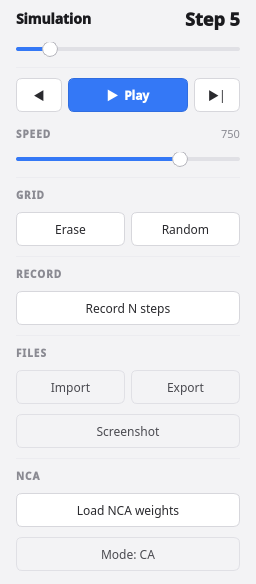
\includegraphics[width=0.8\linewidth]{img/disenoSoftware/ui_main_simulator.png}
			\caption{Controles de evolución.}
			\label{fig:ui_main_simulator}
		\end{subfigure}
		\begin{subfigure}{0.4 \textwidth}
			\centering
			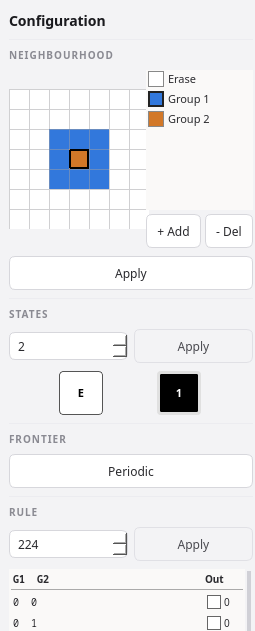
\includegraphics[width=0.8\linewidth]{img/disenoSoftware/ui_main_config.png}
			\caption{Controles de configuración.}
			\label{fig:ui_main_config}
		\end{subfigure}
	\end{figure}
	
	\item \textbf{Pestaña de entrenamiento}
	
	Esta pestaña permite al usuario entrenar el autómata celular neuronal dado un conjunto de datos, tal como se muestra en la figura \ref{fig:ui_training}. 
	
	\begin{figure}[H]
		\centering
		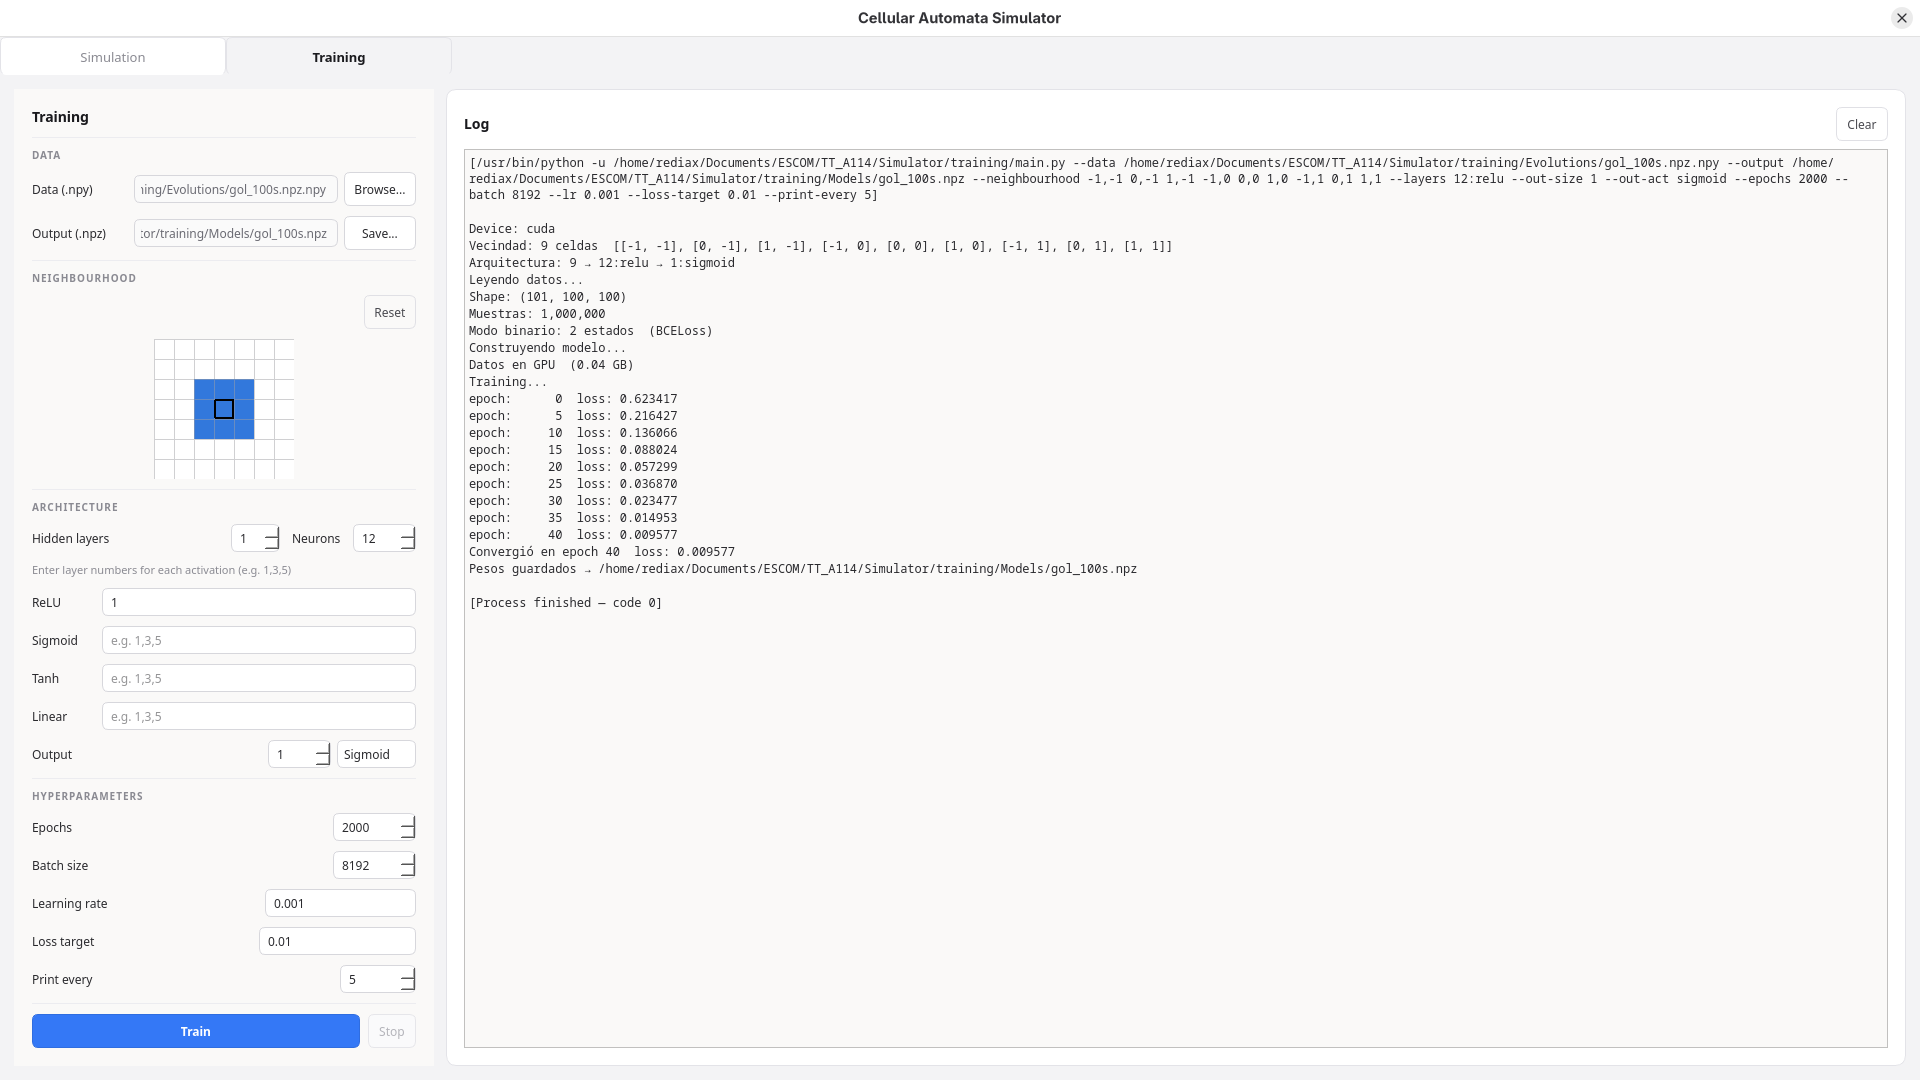
\includegraphics[width=0.9\linewidth]{img/disenoSoftware/ui_training.png}
		\caption{Interfaz de usuario. Pestaña de entrenamiento.}
		\label{fig:ui_training}
	\end{figure}
	
	La primera sección permite realizar la configuración, que incluye los datos de entrenamiento (una o varias evoluciones y el archivo de pesos), la vecindad y la condición de frontera, el número de capas ocultas y las funciones de activación de cada capa, así como la definición de hiperparámetros como el número de épocas, el tamaño del lote, la tasa de aprendizaje y su reducción, la pérdida objetivo y la semilla (ver figura \ref{fig:ui_training_config}). La segunda parte muestra únicamente los registros del entrenamiento. 
	
		\begin{figure}[H]
		\centering
		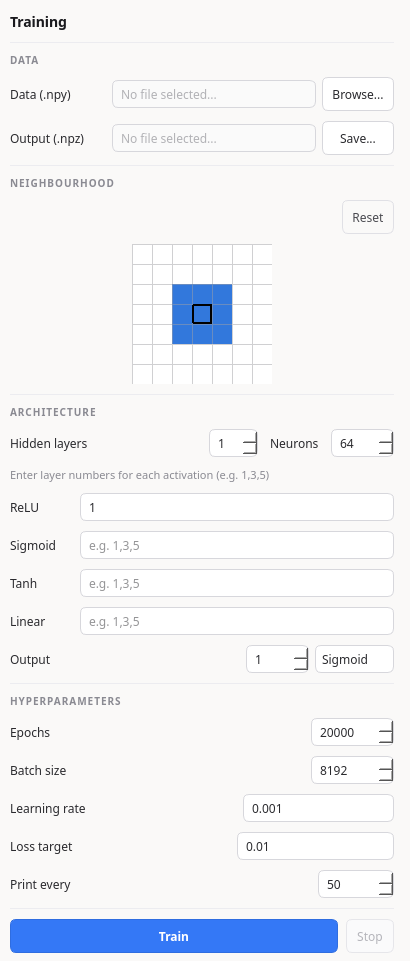
\includegraphics[width=0.8\linewidth]{img/disenoSoftware/ui_training_config.png}
		\caption{Controles de definición de entrenamiento.}
		\label{fig:ui_training_config}
	\end{figure}
\end{itemize}

		
	\chapter{Implementación}


Durante el siguiente capítulo se explora el proceso de implementación de software. Se describe como fueron usadas las tecnologías, las versiones requeridas de las herramientas utilizadas, la estructura del proyecto, el proceso de entrenamiento de la red neuronal y termina con la validación del software, analizando las evoluciones obtenidas.

\section{Entorno de desarrollo}

El simulador se construyó mediante tres entornos de ejecución independientes; cada uno está asociado a una parte fundamental del proyecto o a una herramienta específica. Estos entornos son: 

\begin{itemize}
	\item \textbf{core}: Implementa el cómputo intensivo para la simulación del autómata celular y su versión neuronal, lo que requiere cálculos matriciales complejos que fueron delegados a CUDA por su alto poder computacional paralelo. 
	
	\item \textbf{GUI}: La interfaz gráfica construida en Python utilizando PyQt5 que tiene instancia con el \textit{binding} del core. 
	
	\item \textbf{training}: Módulo de entrenamiento neuronal ejecutado en PyTorch como un proceso desacoplado.
	
\end{itemize}

El sistema fue desarrollado y probado en \textit{Fedora Linux 44 Workstation Edition} con una GPU \textit{NVIDIA} compatible con CUDA. Adicionalmente, en la tabla \ref{table:entorno_global} se describen las versiones requeridas de las herramientas utilizadas.

\begin{table}[H]
    \centering
    \begin{tabular}{l|l}
        \hline
        \textbf{Herramienta} & \textbf{Versión} \\ \hline
        Sistema operativo & Fedora Linux 44 \\ \hline
        Compilador C++ & GCC 15 (\textit{host compiler} para \texttt{nvcc}) \\ \hline
        CUDA Toolkit & 13.2 \\ \hline
        CMake & $\geq$ 3.15 \\ \hline
        Python & 3.14 \\ \hline
        Pybind11 & última versión estable \\ \hline
        PyQt5 & 5.15 \\ \hline
        NumPy & $\geq$ 1.24 \\ \hline
        SciPy & $\geq$ 1.10 \\ \hline
        PyTorch & 2.x con soporte CUDA \\ \hline
    \end{tabular}
    \caption{Versiones de las herramientas del entorno global.}
    \label{table:entorno_global}
\end{table}

\subsection{core}

El módulo de \textit{core} implementa ambos autómatas celulares en C++17 y CUDA. Estos se exponen a Python mediante \textit{bindings}. Se compilan y generan los archivos \texttt{CA.cpython-*.so} y \texttt{NCA.cpython-*.so} que posteriormente son importados por GUI como un módulo nativo.

\begin{itemize}
    \item \textbf{Lenguajes}: C++17 para la lógica y los \textit{bindings}. CUDA C++17 para los \textit{kernels} del dispositivo.
    \item \textbf{Sistema de \textit{build}}: CMake (El compilador para \texttt{nvcc} se fija a GCC 15, ya que HCC 16 no es compatible con CUDA 13.2).
    \item \textbf{Dependencias}: \texttt{pybind11} (instalado en un entorno virtual local), \texttt{CUDAToolkit} y encabezados de Python.
    \item \textbf{Arquitectura GPU}: la opción \texttt{CMAKE\_CUDA\_ARCHITECTURES native} permite que el compilador detecte la \textit{Compute Capability} de la GPU presente al momento de la compilación.
\end{itemize}

El proceso de compilación y exportación del binding al directorio GUI se automatiza mediante el código \texttt{core/bind.sh}. Este \textit{script} activa el entorno virtual, ejecuta CMake, invoca \texttt{make} y copia el artefacto en el directorio de la GUI.

\subsection{GUI}

La interfaz gráfica se desarrolla en Python sobre PyQt5. Es el único medio de interacción con el usuario. 

\begin{itemize}
    \item \textbf{Lenguaje}: Python 3.14.
    \item \textbf{\textit{Framework} gráfico}: PyQt5 (\textit{bindings} de Qt 5.15). Elegido por su modelo de señales y su soporte estable de \texttt{QImage} para el renderizado del espacio celular.
    \item \textbf{Dependencias numéricas}: NumPy para el manejo del arreglo del espacio celular; SciPy para la exportación al formato \texttt{.mat}.
    \item \textbf{Módulo nativo}: \texttt{CA.cpython-*.so} y \texttt{NCA.cpython-*.so}.
\end{itemize}

\subsection{training}

El entorno de entrenamiento es independiente de la GUI y del módulo nativo. No requiere CUDA en tiempo de compilación, ya que PyTorch gestiona el acceso a la GPU en tiempo de ejecución.

\begin{itemize}
    \item \textbf{Lenguaje}: Python 3.x.
    \item \textbf{\textit{Framework} de aprendizaje profundo}: PyTorch 2.x con soporte CUDA. La elección frente a TensorFlow o JAX se justifica por la facilidad de prototipado y el control explícito sobre el entrenamiento.
    \item \textbf{Invocación}: El \textit{script} principal \texttt{training/main.py} se ejecuta de forma independiente o como subproceso lanzado por la pestaña de entrenamiento de la GUI.
\end{itemize}
	\section{Estructura del proyecto}

El proyecto se organiza en tres directorios principales equivalentes a los tres entornos descritos en la sección anterior. Esto asegura el aislamiento de dependencias y la claridad en la lectura dentro del repositorio.

\begin{forest}
	for tree={
		font=\ttfamily,
		grow'=0,
		folder,           
		l sep=1.5em,  
		s sep=2pt,        
	}
	[Simulator/
	[\fitem{core/}{\# C++17/CUDA + bindings pybind11}]
	[\fitem{GUI/}{\# Aplicación PyQt5}]
	[\fitem{training/}{\# Scripts de entrenamiento en PyTorch}]
	]
\end{forest}

\subsection{Directorio core}

Contiene la implementación de bajo nivel del autómata celular y del autómata celular neuronal.

\begin{table}[H]
    \centering
    \begin{tabular}{c|p{0.52\linewidth}}
        \hline
        \textbf{Archivo} & \textbf{Responsabilidad} \\ \hline
        \texttt{ca.h} / \texttt{ca.cu} & Definición e implementación del autómata celular clásico en CUDA. \\ \hline
        \texttt{nca.h} / \texttt{nca.cu} & Definición e implementación del autómata celular neuronal. \\ \hline
        \texttt{bindings/python\_module.cpp} & Capa pybind11 que expone las clases \texttt{CA} y \texttt{NCA} al intérprete de Python. \\ \hline
        \texttt{CMakeLists.txt} & Configuración del \textit{build} con CMake. \\ \hline
        \texttt{bind.sh} & \textit{Script} de automatización. \\ \hline
        \texttt{requirements.txt} & Dependencia única: \texttt{pybind11}. \\ \hline
        \texttt{build/} & Directorio generado por CMake (no versionado). \\ \hline
        \texttt{venv\_bind/} & Entorno virtual local para el proceso de compilación. \\ \hline
    \end{tabular}
    \caption{Contenido del directorio \texttt{core/}.}
\end{table}

\subsection{Directorio GUI}

Implementa la aplicación gráfica completa siguiendo el patrón Modelo-Vista-Controlador descrito en la sección \ref{sec:arquitectura}.

\begin{table}[H]
    \centering
    \begin{tabular}{ p{0.4\textwidth} | p{0.54\textwidth}}
        \hline
        \textbf{Ruta} & \textbf{Responsabilidad} \\ \hline
        \texttt{main.py} & Instancia \texttt{QApplication} y \texttt{MainWindow}. \\ \hline
        \texttt{models/}  \texttt{cellularAutomaton.py} & \textit{Wrapper} de Python sobre la clase \texttt{CA} expuesta por pybind11. \\ \hline
        \texttt{models/}  \texttt{neuralCellularAutomaton.py} & \textit{Wrapper} de Python sobre la clase \texttt{NCA}. \\ \hline
        \texttt{controllers/}  \texttt{SimulationController.py} & Controlador principal. Coordina los \textit{widgets}, el modelo y el \textit{prefetch} asíncrono. \\ \hline
        \texttt{controllers/}  \texttt{SimulationConfig.py} & Encapsulamiento de la configuración del autómata. \\ \hline
        \texttt{ui/}  \texttt{MainWindow.py} & Ventana principal. Contiene un \texttt{QTabWidget} con las pestañas de simulación y entrenamiento. \\ \hline
        \texttt{ui/}  \texttt{ControlPane.py} & Panel izquierdo de la pestaña de simulación: reproducción, paso, retroceso, borrado, aleatorización y velocidad. \\ \hline
        \texttt{ui/}  \texttt{SimulationWidget.py} & \textit{Widget} central. Renderiza la cuadrícula con \texttt{QImage} en formato indexado y emite señales de \textit{click}. \\ \hline
        \texttt{ui/}  \texttt{ConfigPane.py} & Panel derecho. Configura vecindad, estados, frontera y regla de transición. \\ \hline
        \texttt{ui/}  \texttt{NeighbourWidget.py} & Editor visual de la vecindad. Soporta múltiples grupos. \\ \hline
        \texttt{ui/}  \texttt{TrainingPane.py} & Pestaña de entrenamiento. Captura hiperparámetros, lanza \texttt{QProcess} y muestra el \textit{log} en tiempo real. \\ \hline
    \end{tabular}
    \caption{Contenido del directorio \texttt{GUI/}.}
\end{table}

\subsection{Directorio training}

Reúne los \textit{scripts} de entrenamiento del autómata celular neuronal, las evoluciones de referencia utilizadas como conjuntos de datos y los modelos entrenados a partir de ellas.

\begin{table}[H]
    \centering
    \begin{tabular}{p{0.2\linewidth}|p{0.7\linewidth}}
        \hline
        \textbf{Archivo /}   \quad \textbf{directorio} & \textbf{Responsabilidad} \\ \hline
        \texttt{scripts/} \texttt{main.py} & \textit{Script} principal. Implementa la extracción de pares (vecindad, objetivo), la construcción dinámica del MLP en PyTorch y el ciclo de entrenamiento. \\ \hline
        \texttt{scripts/} \texttt{test.py} & Implementa en NumPy el paso del autómata celular neuronal y compara su evolución con la regla exacta del juego de la vida. \\ \hline
        \texttt{scripts/} \texttt{png\_to\_\allowbreak evolution.py} & Convierte una secuencia de imágenes PNG segmentadas en una evolución con el formato \texttt{(T, H, W)} en \texttt{.npy}/\texttt{.mat}. \\ \hline
        \texttt{CA/} & Evoluciones de referencia, una carpeta por experimento: las reglas del juego de la vida (\texttt{evo} para entrenamiento, \texttt{base} como condición de prueba), \texttt{Sandpile/}, \texttt{LangtonAnt/}, \texttt{FLAME3/}, \texttt{SEVIR/} y \texttt{Physarum/}. \\ \hline
        \texttt{NCA/} & Pesos entrenados (\texttt{.npz}) por experimento, las evoluciones que producen (\texttt{t\_*}) y los resultados de los barridos; \texttt{ga\_runs/} contiene la búsqueda genética. \\ \hline
        \texttt{notebooks/} & Un \textit{notebook} por experimento: de Python (\texttt{.ipynb}) para convertir los datos externos en evoluciones (FLAME~3, SEVIR y \textit{Physarum}) y de Wolfram Mathematica (\texttt{.nb}) para el análisis y las figuras (juego de la vida, \textit{sandpile}, hormiga de Langton y FLAME~3). \\ \hline
        \texttt{Dataset/} & Datos crudos descargados (no versionado). \\ \hline
    \end{tabular}
    \caption{Contenido del directorio \texttt{training/}.}
\end{table}

\subsection{Flujo de artefactos entre directorios}

El flujo de artefactos entre directorios es el siguiente:

\begin{enumerate}
    \item El \textit{build} en \texttt{core/build/} produce \texttt{CA.cpython-*.so} (con las clases \texttt{CA} y \texttt{NCA}), que se copia al directorio \texttt{GUI/}.
    \item La GUI registra evoluciones mediante el botón de grabación de \texttt{ControlPane} y las exporta a \texttt{.npy}/\texttt{.mat} en cualquier ubicación, típicamente \texttt{training/CA/}.
    \item El \textit{script} de entrenamiento lee dichos archivos y produce un \texttt{.npz} con pesos, sesgos y metadatos.
    \item La GUI carga el \texttt{.npz} desde \texttt{SimulationController} y cambia al modo NCA para reproducir la evolución aprendida.
\end{enumerate}

Este flujo unidireccional garantiza que los tres entornos puedan evolucionar de forma independiente: un cambio en el módulo nativo no requiere reentrenar, y un cambio en el entrenamiento no requiere recompilar.

	\section{Entrenamiento del modelo}

El entrenamiento del autómata celular neuronal consiste en ajustar los pesos y sesgos del perceptrón multicapa para que, dado el vector de estados en la vecindad de una celda en el instante $t$, produzca como salida el estado de esa misma celda en el instante $t+1$. 

Esta sección describe la implementación concreta del \textit{pipeline} de entrenamiento: la preparación del conjunto de datos, la construcción dinámica del modelo, el ciclo de optimización, la persistencia de los pesos y la integración con la interfaz gráfica.

\subsection{Preparación del conjunto de datos}

El entrenamiento parte de una evolución registrada previamente desde la GUI o generada por una utilidad externa. El archivo se almacena en formato NumPy con \textit{shape} $(T, H, W)$ y \texttt{dtype} entero, donde $T$ es el número de pasos temporales registrados.

A partir de esta evolución se extraen pares de entrenamiento a nivel de celda, no a nivel de imagen. Para cada celda $(x, y)$ en cada instante $t \in [0, T-1)$ se construye:

\begin{itemize}
    \item \textbf{Entrada} $X_{t,x,y}$: vector de tamaño $N_{\text{vec}}$ que concatena el estado de las celdas indicadas por la vecindad relativa a $(x, y)$ en el instante $t$. Las coordenadas se resuelven con condición de frontera periódica (módulo $H$ y $W$).
    \item \textbf{Salida esperada} $Y_{t,x,y}$: estado de la celda $(x, y)$ en el instante $t+1$.
\end{itemize}

Esta vectorización transforma una evolución de $T$ pasos sobre una grilla $H \times W$ en un conjunto de $T \cdot H \cdot W$ muestras independientes, lo que multiplica la cantidad de datos por celdas evaluadas y permite entrenar con \textit{batches} grandes sin requerir múltiples evoluciones.

\subsection{Construcción dinámica del modelo}

La arquitectura del perceptrón multicapa no está fijada en el código: se determina en tiempo de ejecución a partir de los argumentos de la línea de comandos (o de la pestaña de entrenamiento de la GUI). El \textit{script} \texttt{training/scripts/main.py} acepta los parámetros resumidos en la tabla \ref{tab:cli-entrenamiento}.

\begin{table}[H]
    \centering
    \begin{tabular}{l|l|p{0.42\linewidth}}
        \hline
        \textbf{Argumento} & \textbf{\textit{Default}} & \textbf{Descripción} \\ \hline
        \texttt{--data} & --- & Archivo \texttt{.npy} con la evolución de entrada. \\ \hline
        \texttt{--output} & \texttt{weights.npz} & Archivo de salida con los pesos entrenados. \\ \hline
        \texttt{--neighbourhood} & --- & Lista de pares \texttt{"dx,dy"} separados por espacio. \\ \hline
        \texttt{--radius} & 1 & Vecindad cuadrada $(2r+1) \times (2r+1)$ si no se especifica \texttt{--neighbourhood}. \\ \hline
        \texttt{--layers} & --- & Capas ocultas con activación, ejemplo \texttt{"64:relu 32:tanh"}. \\ \hline
        \texttt{--hidden} & 64 & Tamaño de capa oculta única (si no se usa \texttt{--layers}). \\ \hline
        \texttt{--out-size} & 1 & Neuronas de la capa de salida. \\ \hline
        \texttt{--out-act} & \texttt{sigmoid} & Activación de la capa de salida. \\ \hline
        \texttt{--epochs} & 20000 & Número máximo de épocas. \\ \hline
        \texttt{--batch} & 8192 & Tamaño de \textit{batch}. \\ \hline
        \texttt{--lr} & 0.001 & Tasa de aprendizaje del optimizador. \\ \hline
        \texttt{--loss-target} & 0.01 & Umbral de pérdida para detención temprana. \\ \hline
        \texttt{--print-every} & 50 & Frecuencia de impresión del \textit{log}. \\ \hline
    \end{tabular}
    \caption{Argumentos CLI del \textit{script} de entrenamiento.}
    \label{tab:cli-entrenamiento}
\end{table}

A partir de estos argumentos se construye un \texttt{torch.nn.Sequential} concatenando capas \texttt{nn.Linear} con la activación correspondiente. Las activaciones soportadas son \texttt{ReLU}, \texttt{Sigmoid}, \texttt{Tanh} y \texttt{Linear} (identidad), las mismas que reconoce el \textit{kernel} CUDA del NCA. La equivalencia de códigos numéricos (\texttt{0=ReLU, 1=Sigmoid, 2=Tanh, 3=Linear}) garantiza que los pesos entrenados sean directamente ejecutables en el dispositivo.

\subsection{Ciclo de optimización}

El entrenamiento sigue un esquema de optimización por descenso de gradiente estocástico con minilotes:

\begin{itemize}
    \item \textbf{Optimizador}: \texttt{torch.optim.Adam} con la tasa de aprendizaje configurada. Se eligió Adam por su robustez frente a la elección inicial de hiperparámetros y por su comportamiento estable en presencia de gradientes ruidosos.
    \item \textbf{Función de pérdida}: error cuadrático medio (\texttt{MSELoss}). Aunque el objetivo es discreto en los autómatas celulares clásicos, el MLP produce salidas continuas y se interpreta el valor de salida mediante umbralización al momento de inferencia.
    \item \textbf{Detención temprana}: el ciclo se interrumpe cuando la pérdida acumulada por época cae por debajo de \texttt{loss\_target}, evitando épocas adicionales innecesarias una vez que el modelo ha convergido.
    \item \textbf{\textit{Logging}}: cada \texttt{print\_every} épocas se imprime el número de época, la pérdida acumulada. Este \textit{log} se captura en tiempo real por la GUI cuando el entrenamiento se lanza desde \texttt{TrainingPane}.
\end{itemize}

\subsection{Persistencia de los pesos}

Al finalizar el entrenamiento, el modelo se almacena en un archivo \texttt{.npz} con la siguiente estructura:

\begin{itemize}
    \item \texttt{weights\_N} y \texttt{biases\_N} por cada capa lineal (con $N$ el índice de capa).
    \item \texttt{layer\_in}, \texttt{layer\_out}: tamaños de entrada y salida.
    \item \texttt{activations}: arreglo de códigos enteros para cada capa.
    \item \texttt{neighbourhood}: lista de desplazamientos relativos utilizada durante el entrenamiento.
\end{itemize}

Este formato es el que espera el método \texttt{on\_load\_nca\_button} de \texttt{SimulationController} y es compatible con la firma del constructor de la clase \texttt{NCA} en el módulo nativo, sin necesidad de transformaciones intermedias.

\subsection{Integración con la interfaz gráfica}

Desde la pestaña de entrenamiento de la GUI, el usuario configura visualmente la vecindad, las capas ocultas, las activaciones y los hiperparámetros. Al pulsar el botón de entrenamiento, la GUI ensambla la línea de comandos equivalente e instancia un \texttt{QProcess} con la \textit{flag} \texttt{-u} de Python, que desactiva el \textit{buffering} de la salida estándar. La salida estándar y de error del subproceso se conecta mediante señales de Qt a un \textit{widget} de \textit{log} que se actualiza en tiempo real.

Esta arquitectura permite que el entrenamiento se ejecute en un proceso completamente independiente del de la GUI: una falla durante el entrenamiento no afecta a la interfaz, y el usuario puede continuar simulando o ajustando la configuración mientras el proceso avanza en segundo plano. Una vez terminado, el archivo \texttt{.npz} resultante puede cargarse desde la pestaña de simulación para intercambiar al modo NCA.

	\section{Validación y pruebas}

La validación del simulador se realiza en tres partes: primero se comprueba el funcionamiento del autómata celular replicando reglas conocidas; después se realiza una verificación numérica del autómata celular neuronal y finalmente se realizan mediciones de rendimiento. Además, se describen las pruebas de interfaz, el manejo de errores y los cambios que requirió el \textit{software} durante la investigación.

\subsection{Validación funcional del autómata celular clásico}

El autómata celular se valida reproduciendo reglas ampliamente documentadas en la literatura y comparando visual y numéricamente la evolución obtenida con la esperada.

Para esto se establece la misma condición inicial en dos diferentes simuladores y se evolucionan bajo las mismas condiciones. Si la diferencia de las evoluciones en cada paso evolutivo es $0$, se infiere que el comportamiento es el mismo, pues sus trayectorias en el espacio de evoluciones son equivalentes.

\subsection{Validación del autómata celular neuronal}

El criterio de validación del entrenamiento es la capacidad del modelo entrenado para replicar la regla original. Para cada regla objetivo se realiza el siguiente procedimiento:

\begin{enumerate}
    \item Generar una evolución de $T$ pasos con el autómata celular clásico.
    \item Entrenar el perceptrón multicapa con dicha evolución.
    \item Cargar los pesos resultantes en el modo NCA del simulador.
    \item Ejecutar una nueva evolución partiendo de la misma configuración inicial y comparar.
\end{enumerate}

La métrica principal es el porcentaje de celdas coincidentes entre las dos evoluciones a lo largo de los $T$ pasos. Una coincidencia superior al 99\% en una vecindad completa se interpreta como que el autómata celular neuronal fue capaz de replicar exitosamente la regla.

\subsection{Pruebas de rendimiento}

Para las pruebas de rendimiento en la simulación se utilizó la regla B3/S23 con una población aleatoria del 50\% de células vivas. El rendimiento se analiza dentro del método \texttt{step()}, que es quien ejecuta el paso evolutivo y se sincroniza con la GPU, y el método \texttt{run()}, que ejecuta $N$ pasos consecutivos.

\begin{table}[H]
    \centering
    \begin{tabular}{c|c|c}
        \hline
        $n$ & \texttt{step()} (pasos/s) & \texttt{run(100)} (pasos/s) \\ \hline
        100  & 345,000 & 102,800 \\ \hline
        500  & 313,000 &   6,500 \\ \hline
        1,000 & 137,000 &   1,800 \\ \hline
        2,000 &  55,400 &     520  \\ \hline
    \end{tabular}
    \caption{Velocidad de evolución medida sobre cuadrículas $n \times n$. \texttt{step()} mide únicamente el \textit{kernel} y el intercambio de \textit{buffers} (sincronización perezosa). \texttt{run()} incluye la copia \textit{device-to-host} por \textit{frame}, que constituye el techo real para la reproducción visible.}
    \label{tab:perf-evolucion}
\end{table}

La caída de \texttt{run()} respecto a \texttt{step()} cuantifica el costo de la transferencia \textit{device-to-host}: en cuadrículas de $2{,}000 \times 2{,}000$ la transferencia domina por encima del cómputo.

\subsubsection{Velocidad de renderizado}

El renderizado se mide en modo \texttt{offscreen} de Qt Platform Abstraction para aislar el costo de dibujar del costo del sistema de ventanas. Se contabiliza el tiempo medio entre \texttt{update()} y la finalización del \textit{repaint}.

\begin{table}[H]
    \centering
    \begin{tabular}{c|c|c}
        \hline
        $n$ & ms / \textit{repaint} & fps \\ \hline
        100  & 0.66 & 1,515 \\ \hline
        500  & 0.89 & 1,125 \\ \hline
        1,000 & 2.83 &  353 \\ \hline
        2,000 & 8.18 &  122 \\ \hline
    \end{tabular}
    \caption{Velocidad de renderizado para distintos tamaños de cuadrícula.}
    \label{tab:perf-render}
\end{table}

Incluso a $2{,}000 \times 2{,}000$ celdas (4 millones de celdas), el renderizado supera los 100 fps, lo que confirma la viabilidad del enfoque basado en \texttt{QImage(Format\_Indexed8)} con una sola llamada a \texttt{drawImage} por \textit{frame}.

\subsection{Pruebas de interfaz}

Las pruebas de la interfaz gráfica se realizaron de forma manual siguiendo guiones derivados de los casos de uso. Los escenarios principales validados son:

\begin{itemize}
    \item Configuración de una regla desde cero: definir estados, vecindad multigrupo y tabla de regla, y verificar la evolución resultante.
    \item Edición interactiva del espacio celular: pintar con el mouse, borrar y aleatorizar, comprobando que la grilla mostrada coincide con el estado interno del autómata.
    \item Importación y exportación de evoluciones: grabar una evolución, exportarla a \texttt{.npy} y \texttt{.mat}, reimportarla y verificar que la secuencia reproducida es idéntica.
    \item Carga de un modelo NCA entrenado y conmutación entre los modos CA y NCA durante la simulación.
    \item Lanzamiento del subproceso de entrenamiento desde la pestaña correspondiente, verificando la captura de la salida en tiempo real y la correcta finalización del archivo \texttt{.npz}.
\end{itemize}

\subsection{Robustez y manejo de errores}

A lo largo del desarrollo se identificaron y resolvieron algunos errores:

\begin{itemize}
    \item \textbf{Errores de CUDA silenciosos}: todas las llamadas a la API de CUDA se envuelven en una macro \texttt{CUDA\_CHECK} que verifica el código de retorno y aborta con un mensaje descriptivo, evitando fallos de segmentación retardados que dificultan la depuración. La macro se omite deliberadamente en los destructores para no propagar excepciones durante la destrucción de los objetos.
    \item \textbf{Tamaño de tabla excesivo}: cambios en \texttt{states} o en \texttt{group\_sizes} pueden generar tablas de regla que excederían los límites técnicos del dispositivo. La capa de \textit{bindings} prevalida $r_{\text{size}} \leq 16{,}777{,}216$ antes de aplicar cualquier cambio.
    \item \textbf{Invalidación del \textit{prefetch}}: el contador \texttt{\_generation} en el controlador descarta de forma segura los \textit{frames} precomputados cuyo trabajo ha quedado obsoleto, evitando inconsistencias visuales.
    \item \textbf{\textit{Mismatch} entre el \textit{driver} y la biblioteca de CUDA}: Incidentes documentados durante el desarrollo recomendaron reiniciar el sistema tras actualizaciones parciales del \textit{driver} NVIDIA.
\end{itemize}

\subsection{Cambios}

Durante el desarrollo de la investigación, estos fueron los cambios requeridos en el \textit{software} que no fueron contemplados:

\begin{itemize}
	\item Se añadió un campo opcional en el módulo de entrenamiento que es la semilla, esto para poder replicar experimentos y, además, para poder realizar múltiples pruebas con diferentes semillas aleatorias.
	\item Se agregó la reducción de la tasa de aprendizaje durante el entrenamiento (\texttt{--lr-schedule}): exponencial, coseno o por estancamiento (\textit{plateau}), debido a que con una tasa constante la pérdida oscilaba sin alcanzar la pérdida objetivo.
	\item Se agregó la codificación \textit{one-hot} de la capa de entrada (\texttt{--one-hot}). El número de estados se guarda en el archivo de pesos (\texttt{one\_hot\_states}) y lo interpretan tanto el \textit{kernel} del autómata celular neuronal como la GUI.
	\item Se agregó la frontera abierta en el entrenamiento (\texttt{--open-boundary}) para sistemas como \textit{sandpile}, en los que lo que sale del espacio se pierde.
	\item El entrenamiento acepta varios archivos de datos, en formato \texttt{.npy} o \texttt{.mat}, cuyas transiciones se juntan en un solo conjunto de datos.
	\item Se agregó el registro de la pérdida y de la tasa de aprendizaje en un archivo CSV (\texttt{--log-csv}) para graficar las curvas de entrenamiento.
\end{itemize}

	\chapter{Replicación de comportamientos conocidos}

Una vez construido, validado e implementado el simulador, el siguiente paso es la experimentación con el objetivo de replicar el comportamiento de sistemas complejos. 

En este capítulo y en el siguiente se exponen seis experimentos realizados con el simulador para entrenar autómatas celulares neuronales, con un análisis paralelo mediante Mathematica. Los experimentos se dividen en dos series:

\begin{enumerate}
	\item \textbf{Replicación de comportamientos conocidos} (este capítulo). Se entrena el autómata celular neuronal con evoluciones de reglas bien conocidas (juego de la vida, \textit{sandpile} y hormiga de Langton) para medir su capacidad de recuperar la regla a partir de la evolución y la vecindad.
	\item \textbf{Replicación de sistemas complejos naturales} (capítulo \ref{chap:naturales}). Se entrena con evoluciones obtenidas de sistemas reales sin una regla de transición conocida: la propagación de un incendio, el movimiento de tormentas y el crecimiento de un moho mucilaginoso. Cada sistema requiere su propio método de limpieza para llevar los datos al formato $(T, n, n)$ del simulador.
\end{enumerate}

El objetivo de esta primera serie de experimentos es replicar el comportamiento de evoluciones conocidas para identificar las capacidades y limitaciones del autómata celular neuronal en entornos controlados. 

Primero se realizan experimentos sobre el juego de la vida de John Conway. Se usa como base la regla B3/S23, se caracteriza la regla y posteriormente se definen los hiperparámetros y las condiciones necesarias para que el autómata celular neuronal pueda replicar (o intentar replicar) el comportamiento de dicha regla. 

Posteriormente se experimenta sobre \textit{sandpile}: un sistema autoorganizado que consiste en una cuadrícula y un generador de arena que, cuando se llena, dispersa la arena en sus vecinos cercanos. 

Finalmente, se replica la hormiga de Langton mediante un autómata celular. La hormiga de Langton es un agente reactivo en un espacio bidimensional que sigue una serie de instrucciones según su posición.
	\section{El juego de la vida}

Para este experimento, se utiliza principalmente la regla B3/S23, de la cual fueron evolucionadas 100 condiciones iniciales aleatorias en un espacio de $100 \times 100$ durante 100 pasos evolutivos para analizar su comportamiento.  

De acuerdo con la figura \ref{fig:life_state_distribution}, la regla B3/S23 produce el estado uno un $16.5\%$ de las veces. La mayoría de los datos se agrupa entre $12.3\%$ y $20.7\%$, donde los porcentajes más grandes corresponden a las configuraciones iniciales aleatorias. Esto se demuestra en la figura \ref{fig:life_all_steps}, donde la proporción del estado uno de todas las evoluciones a través del tiempo decrece hasta estabilizarse, comportamiento característico del atractor de dicha regla.

\begin{figure}[htbp]
	\centering
	\begin{subfigure}[b]{0.49\textwidth}
		\centering
		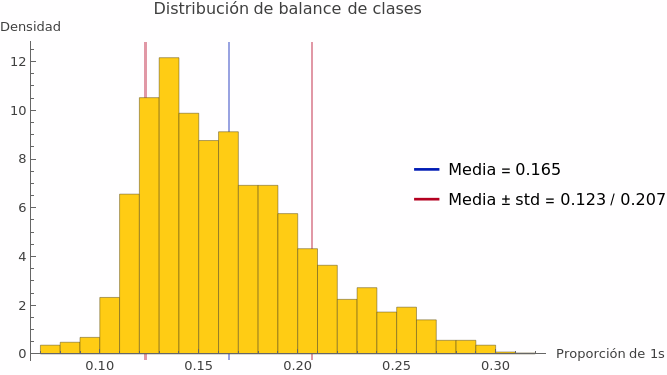
\includegraphics[width=\linewidth]{img/experimentacion/duplicacion/gol/life_state_distribution.png}
		\caption{Histograma de distribución de la clase 1. Media de $16.5$ y desviación estándar de $4.2$.}
		\label{fig:life_state_distribution} 
	\end{subfigure}%
	\hfill % Añade espacio horizontal flexible entre las figuras
	\begin{subfigure}[b]{0.49\textwidth}
		\centering
		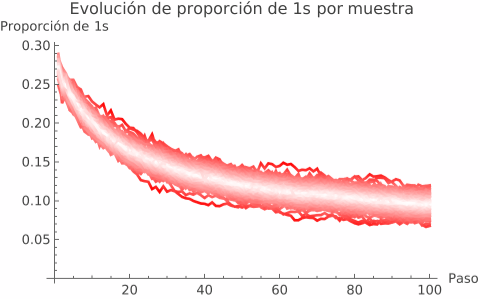
\includegraphics[width=\linewidth]{img/experimentacion/duplicacion/gol/life_all_steps.png}
		\caption{Proporción de unos a lo largo del tiempo de todas las muestras.}
		\label{fig:life_all_steps}
	\end{subfigure}
	\caption{Resultados estadísticos del conjunto de pruebas para la regla B3/S23.}
\end{figure}

Por otro lado, dado que la salida de cada paso evolutivo es la entrada del siguiente, también se analiza el desbalance de entradas, es decir, la frecuencia con la que aparecen diferentes patrones. Para esto, utilizaremos la nomenclatura $CxNy$ que cuenta el número de unos que aparecen en el centro ($C$) y en el exterior ($N$).

En la figura \ref{fig:life_pattern_count} se muestran las frecuencias de aparición de todos los patrones en el mismo conjunto de datos. La regla B3/S23 no genera mucha vida dentro de las comunidades, lo que causa un desbalance de entradas. Los patrones con menor frecuencia de aparición son $C1N8$ y $C0N8$, que suman menos del $0.02\%$, lo que causa un problema de representación o sesgo de muestra.

\begin{figure}[H]
	\centering
	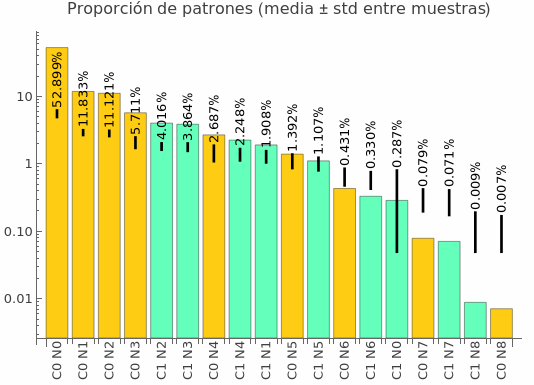
\includegraphics[width=0.7\linewidth]{img/experimentacion/duplicacion/gol/life_pattern_count.png}
	\caption{Distribuciones de probabilidad de los patrones en la regla B3/S23.}
	\label{fig:life_pattern_count}
\end{figure}

Para evitar este sesgo, se proponen dos soluciones: (1) realizar un sobremuestreo de los datos menos frecuentes o (2) modificar la función de costo para penalizar en mayor medida los errores en patrones poco representados. Las pruebas a continuación se realizan con una pérdida objetivo exigente con la intención de encontrar configuraciones capaces de replicar el comportamiento de forma exacta.

\subsection{Capacidad de replicación}

Se usa la siguiente nomenclatura:
\[
\text{número de capas}:\text{número de neuronas}:\text{función de activación}
\]
para especificar la composición de la red neuronal. 

Fueron probadas 10 combinaciones de funciones de activación, de las cuales una sola converge en menos de 1,000 épocas. 
En la tabla \ref{tab:nca_gol_funciones_1} se observan los resultados. La falta de convergencia puede deberse al tamaño de la red neuronal o a la pérdida objetivo utilizada. 

\begin{table}[h]
	\centering
	\begin{tabular}{llrrr}
		\toprule
		\textbf{Capa Oculta} & \textbf{Capa Salida} & \textbf{Épocas} & \textbf{Pérdida} & \textbf{Tiempo} \\
		\midrule
		1:4:ReLU & 2:Linear & 122 & 0.000098 & 4.64 s \\
		1:4:TanH & 1:Sigmoid & 1,000 & 0.052895 & 40.19 s\\
		1:4:TanH & 2:Linear & 1,000 & 0.079425 & 36.52 s \\
		1:4:Sigmoid & 2:Linear & 1,000 & 0.159343 & 36.71 s \\
		1:4:Sigmoid & 1:Sigmoid & 1,000 & 0.159343 & 39.37 s \\
		1:4:ReLU & 2:TanH & 1,000 &  0.179589 & 38.65 s \\
		1:4:ReLU & 1:Sigmoid & 1,000 & 0.269196 & 38.16 s\\
		1:4:Linear & 1:Sigmoid & 1,000 & 0.297529 & 39.12 s \\
		1:4:Linear & 2:Linear & 1,000 & 0.297529 & 34.75 s  \\
		1:4:ReLU & 2:Sigmoid & 1,000 & 0.374756 & 37.55 s \\
		\bottomrule
	\end{tabular}
	\caption{Comparativa de rendimiento con múltiples hiperparámetros de la regla B3/S23: pérdida objetivo 0.0001, límite de épocas: 1,000,
		tamaño del lote: 8,192, tasa de aprendizaje: 0.001, semilla aleatoria: 42.}
	\label{tab:nca_gol_funciones_1}
\end{table}

Al incrementar el número de capas ocultas y de neuronas, se observa en la tabla \ref{tab:nca_gol_funciones_2} que existen cuatro nuevas configuraciones que alcanzan la convergencia. Adicionalmente, en la figura \ref{fig:gol_funciones_2} observamos que el estancamiento ocurre en las primeras 12 épocas, lo que sugiere un problema de la combinación de funciones de activación más que una limitación de la tasa de aprendizaje. 

\begin{table}[h]
	\centering
	\begin{tabular}{llrr}
		\toprule
		\textbf{Capa Oculta} & \textbf{Capa Salida} & \textbf{Épocas} & \textbf{Pérdida}\\
		\midrule
		4:8:ReLU & 2:Linear & 18 & 0.000087 \\
		4:8:TanH & 1:Sigmoid & 51 & 0.000097 \\
		4:8:TanH & 2:Linear & 35 & 0.000097 \\
		4:8:Sigmoid & 2:Linear & 79 & 0.000095 \\
		4:8:Sigmoid & 1:Sigmoid & 1,000 & 0.159342 \\
		4:8:ReLU & 2:TanH & 1,000 & 0.126928 \\
		4:8:ReLU & 1:Sigmoid & 133 & 0.000096 \\
		4:8:Linear & 1:Sigmoid & 1,000 & 0.297542 \\
		4:8:Linear & 2:Linear & 1,000 & 0.297544 \\
		4:8:ReLU & 2:Sigmoid & 1,000 & 0.374756 \\
		\bottomrule
	\end{tabular}
	\caption{Comparativa de rendimiento con múltiples hiperparámetros de la regla B3/S23: pérdida objetivo 0.0001, límite de épocas: 1,000,
		tamaño del lote: 8,192, tasa de aprendizaje: 0.001, semilla aleatoria: 42.}
	\label{tab:nca_gol_funciones_2}
\end{table}

\begin{figure}[H]
	\centering
	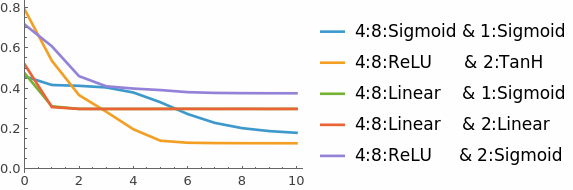
\includegraphics[width=0.75\linewidth]{img/experimentacion/duplicacion/gol/gol_funciones_2.png}
	\caption{Registro de pérdida obtenida en las primeras 12 épocas de las configuraciones sin convergencia de la tabla \ref{tab:nca_gol_funciones_2}.}
	\label{fig:gol_funciones_2}
\end{figure}

Queda demostrado que un autómata celular neuronal puede aprender el comportamiento de una regla ya conocida con una pérdida de 0.0001. Para fines de esta investigación, se omiten las configuraciones no convergentes.

\subsection{Aprendizaje de reglas similares}

De acuerdo con la figura \ref{fig:life_pattern_count}, las probabilidades de aparición de los patrones $C0N8$ y $C1N8$ son menores que $0.02\%$. La siguiente prueba busca identificar la relación entre la pérdida objetivo y la regla aprendida. Para esto, se entrena la regla B3/S23 con diferentes pérdidas objetivo y se identifica cómo esos patrones infrecuentes afectan el aprendizaje.

Cabe mencionar que aunque las reglas del juego de la vida son semitotalísticas, existe la posibilidad de que la regla aprendida no lo sea, es decir, que el autómata celular neuronal sí haga distinción entre dos patrones que conduzcan al mismo comportamiento. Por ejemplo, podemos generar de ocho formas diferentes el patrón $C0N1$:
\[
 \left[ \begin{matrix} 1 & 0 & 0 \\ 0 & 0 & 0 \\ 0 & 0 & 0 \end{matrix} \right] = 
 \left[ \begin{matrix} 0 & 1 & 0 \\ 0 & 0 & 0 \\ 0 & 0 & 0 \end{matrix} \right] = \dots = 
 \left[ \begin{matrix} 0 & 0 & 0 \\ 0 & 0 & 0 \\ 0 & 0 & 1 \end{matrix} \right]
\]
 pero, a falta de exposición a todas las posibles configuraciones, la red neuronal puede distinguir patrones, lo que convierte a la regla en una arbitraria.
 
Las reglas semitotalísticas son un subconjunto de las reglas arbitrarias. Para verificar que la regla aprendida coincida con todas las posibles configuraciones de los patrones, se diseñó la configuración inicial de la figura \ref{fig:test}, la cual se evoluciona un paso y se comparan los centros de cada subespacio de $3 \times 3$. 

\begin{figure}[H]
	\centering
	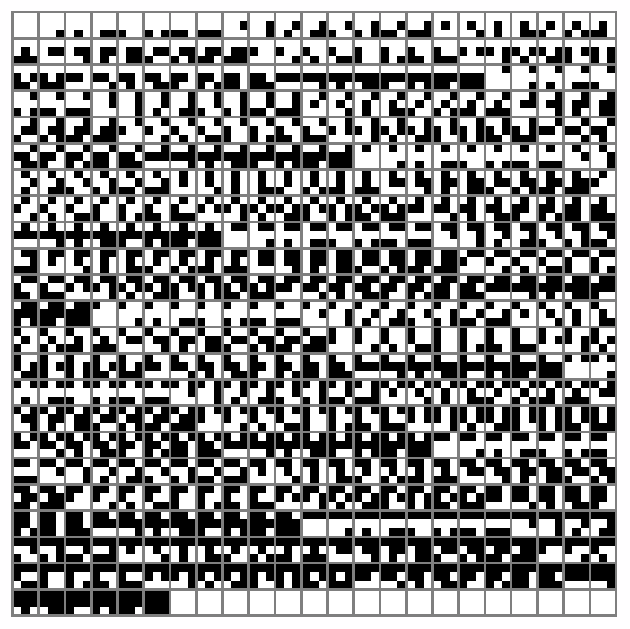
\includegraphics[width=0.6\linewidth]{img/experimentacion/duplicacion/gol/test.png}
	\caption{Espacio que contiene todas las configuraciones posibles ($2^9 = 512$) de 2 estados en 9 células.}
	\label{fig:test}
\end{figure}

Los autómatas celulares neuronales que utilizaron las pérdidas objetivo de 0.2 y 0.3 aprendieron la regla 0 (ver figura \ref{fig:b3s23_loss}). Podemos concluir que esta configuración es estable porque, aunque existan patrones de baja frecuencia como $C0N8$ y $C1N8$, sigue siendo capaz de replicar el comportamiento con una pérdida objetivo de $0.1$. Una hipótesis es que la red neuronal se inicializa generando ceros y, como casi nunca recibe esas entradas, sus salidas para ellas se mantienen en ese valor. 

\begin{figure}[H]
	\centering
	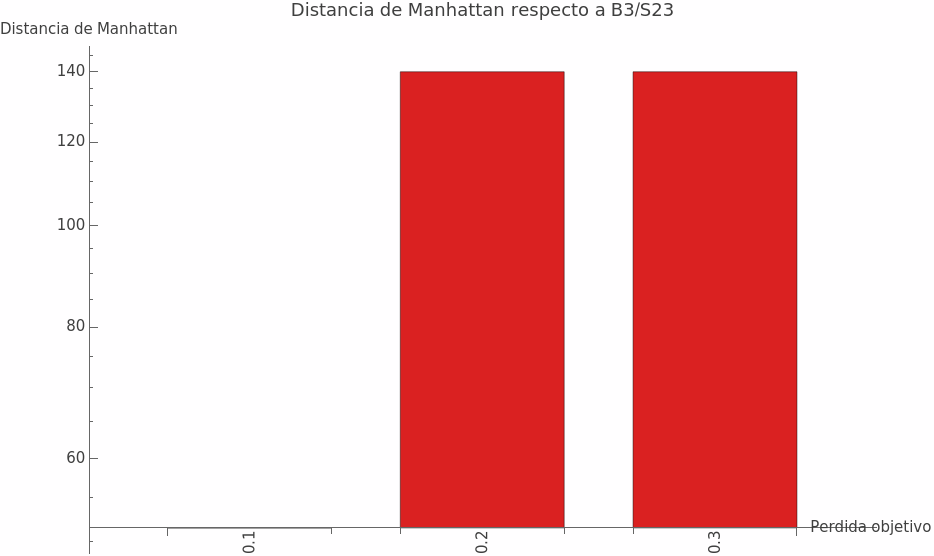
\includegraphics[width=0.6\linewidth]{img/experimentacion/duplicacion/gol/b3s23_loss.png}
	\caption{Distancia Manhattan de los vectores de regla de múltiples pérdidas objetivo comparados con B3/S23.}
	\label{fig:b3s23_loss}
\end{figure}


A continuación, se replica el experimento para las siguientes reglas \textit{life-like}: B3/S238, B38/S238 y B3/S236.

Para la regla B3/S238 (figura \ref{fig:b3s238_loss}), el autómata celular neuronal aprende una regla que difiere únicamente en un elemento (con una pérdida objetivo entre 0.03 y 0.1). Esta diferencia corresponde al patrón $C1N8$, el cual solo tiene una posible representación:
\[
\left[
\begin{matrix}
	1 & 1 & 1 \\
	1 & 1 & 1 \\
	1 & 1 & 1 
\end{matrix}
\right]
\]

\begin{figure}[H]
	\centering
	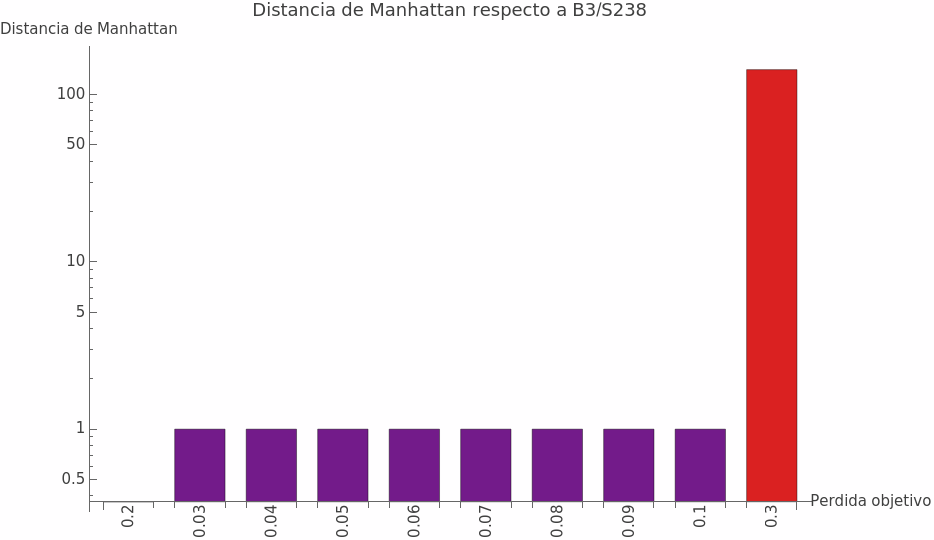
\includegraphics[width=.6\linewidth]{img/experimentacion/duplicacion/gol/b3s238_loss.png}
	\caption{Distancia Manhattan de los vectores de regla de múltiples pérdidas objetivo comparados con B3/S238.}
	\label{fig:b3s238_loss} 
\end{figure}

Como la regla aprendida considera todas las permutaciones del patrón $C1N8$, esto significa que aprendió una regla semitotalística que ignora la supervivencia con 8 vecinos. Su regla aprendida equivale a B3/S23. Esto lo corroboramos con la figura \ref{fig:b3s238_vector}, en donde se muestra la única diferencia entre ambas reglas y cómo fue omitida durante el entrenamiento. 

\begin{figure}[H]
	\centering
	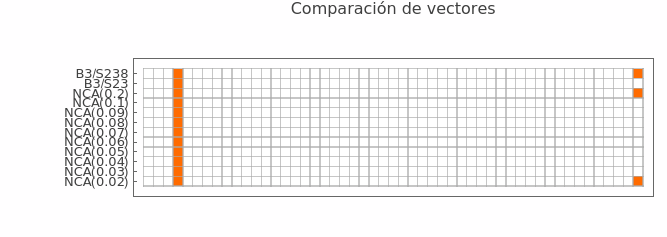
\includegraphics[width=.8\linewidth]{img/experimentacion/duplicacion/gol/b3s238_vector.png}
	\caption{Últimos 50 elementos de los vectores de regla de B3/S238, B3/S23 y los aprendidos por el autómata celular neuronal.}
	\label{fig:b3s238_vector} 
\end{figure}

Con la regla B38/S238 (figura \ref{fig:b38s238_loss}) se aprenden 2 comportamientos diferentes: B3/S238 y B3/S23, como se observa en la figura \ref{fig:b38s238_vector}.

\begin{figure}[H]
	\centering
	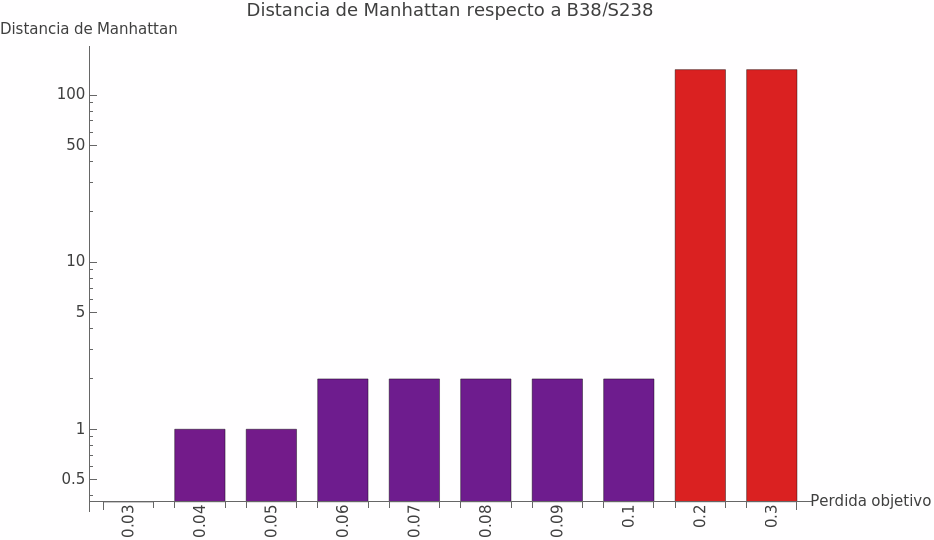
\includegraphics[width=.6\linewidth]{img/experimentacion/duplicacion/gol/b38s238_loss.png}
	\caption{Distancia Manhattan de los vectores de regla de múltiples pérdidas objetivo comparados con B38/S238.}
	\label{fig:b38s238_loss} 
\end{figure}

\begin{figure}[H]
	\centering
	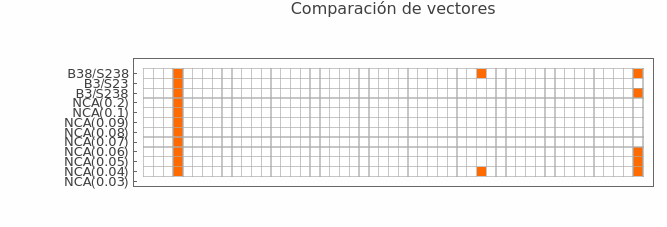
\includegraphics[width=.8\linewidth]{img/experimentacion/duplicacion/gol/b38s238_vector.png}
	\caption{Últimos 50 elementos de los vectores de regla de B38/S238, B3/S23, B3/S238 y los aprendidos por el autómata celular neuronal.}
	\label{fig:b38s238_vector} 
\end{figure}

En la regla B3/S236 (figura \ref{fig:b3s236_loss}), con una pérdida objetivo de 0.2 difieren 32 elementos, de los cuales 28 sustituyeron el 1 por 0 (figura \ref{fig:b3s236_02_10}) y 4 al revés (figura \ref{fig:b3s236_02_01}). El primer conjunto corresponde al patrón $C1N6$, mientras que los 4 restantes necesitan otros 4 patrones adicionales para capturar a $C1N7$. Por esta razón, la regla aprendida no es semitotalística: hace distinción entre elementos de su vecindad.

\begin{figure}[H]
	\centering
	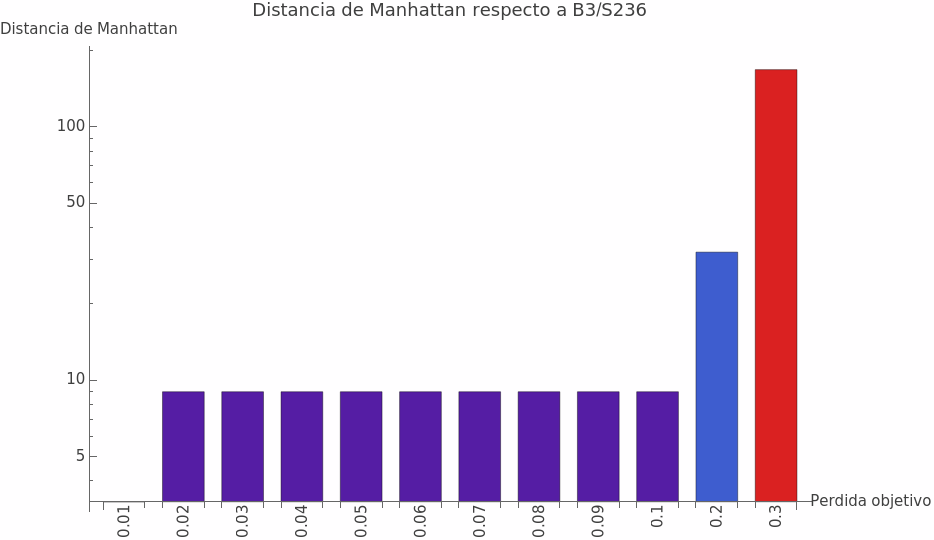
\includegraphics[width=.75\linewidth]{img/experimentacion/duplicacion/gol/b3s236_loss.png}
	\caption{Distancia Manhattan de los vectores de regla de múltiples pérdidas objetivo comparados con B3/S236.}
	\label{fig:b3s236_loss} 
\end{figure}

\begin{figure}[htbp]
	\centering
	\begin{subfigure}[b]{0.5\textwidth}
		\centering
		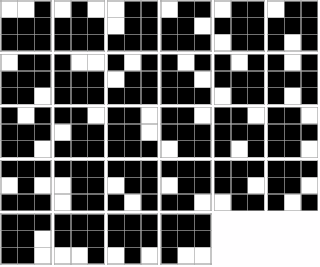
\includegraphics[width=0.7\linewidth]{img/experimentacion/duplicacion/gol/b3s236_02_10.png}
		\caption{Se intercambió 1 por 0 en $C1N6$.}
		\label{fig:b3s236_02_10} 
	\end{subfigure}%
	\hfill % Añade espacio horizontal flexible entre las figuras
	\begin{subfigure}[b]{0.5\textwidth}
		\centering
		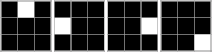
\includegraphics[width=0.5\linewidth]{img/experimentacion/duplicacion/gol/b3s236_02_01.png}
		\caption{Se intercambió 0 por 1.}
		\label{fig:b3s236_02_01}
	\end{subfigure}
	\caption{Patrones que difieren entre B3/S236 y el autómata celular neuronal con una pérdida objetivo de 0.2.}
\end{figure}

El resto de reglas aprendidas erróneamente (con pérdidas objetivo de 0.02 a 0.1) diferencian los patrones de las figuras \ref{fig:b3s236_03_10} y \ref{fig:b3s236_03_01}. Ambos patrones se encuentran completos ($C1N7$ y $C1N8$), por lo que la célula sobrevive con 7 y 8 vecinos, es decir, aprendió la regla B3/S23678.

\begin{figure}[htbp]
	\centering
	\begin{subfigure}[b]{0.5\textwidth}
		\centering
		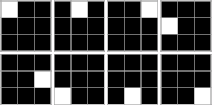
\includegraphics[width=0.7\linewidth]{img/experimentacion/duplicacion/gol/b3s236_03_10.png}
		\caption{Se intercambió 0 por 1 en $C1N7$.}
		\label{fig:b3s236_03_10} 
	\end{subfigure}%
	\hfill % Añade espacio horizontal flexible entre las figuras
	\begin{subfigure}[b]{0.5\textwidth}
		\centering
		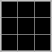
\includegraphics[width=0.17\linewidth]{img/experimentacion/duplicacion/gol/b3s236_03_01.png}
		\caption{Se intercambió 0 por 1 en $C1N8$.}
		\label{fig:b3s236_03_01}
	\end{subfigure}
	\caption{Patrones que difieren entre B3/S236 y el autómata celular neuronal con pérdidas objetivo de 0.02 a 0.1.}
\end{figure}

\subsection{Efecto del tamaño de la vecindad}

Experimentar con reglas ya conocidas implica conocer toda la configuración necesaria de ese sistema en específico. Esto no ocurre en fenómenos reales, donde no conocemos el número de estados, la función de transición o, específicamente para este experimento, la vecindad que define el sistema. Los siguientes experimentos tienen el propósito de identificar cómo afecta el desconocimiento de la vecindad en un sistema complejo al momento de intentar replicar el comportamiento de la regla B3/S23.

Dada la vecindad de la regla, definimos las siguientes pruebas: (1) eliminación de una célula exterior, (2) eliminación de la célula central, (3) incremento del tamaño de la vecindad y (4) sustitución de elementos de la vecindad. Con esto se busca identificar un método de selección de vecindad que nos permita extraer el comportamiento esencial de un sistema complejo.

La vecindad semitotalística se divide en dos subvecindades: el centro y los bordes. Dado que el valor de la subvecindad de los bordes está dado por la sumatoria, cada uno de ellos tiene la misma relevancia, por lo que solo es necesario realizar pruebas ignorando uno de esos elementos. La tabla \ref{tab:vecindad_ajuste_16x16} muestra las pérdidas finales obtenidas bajo diferentes configuraciones, todas mayores a 0.1. 

\begin{table}[H]
	\centering
	\small
	\begin{tabular}{ccccccc}
		\toprule
		& & \textbf{ReLU} & \textbf{TanH} & \textbf{TanH} & \textbf{ReLU} &  \\
		\textbf{Tasa} & \textbf{Lote} & \textbf{2:Linear }&  \textbf{1:Sigmoid }& \textbf{2:Linear  }& \textbf{1:Sigmoid} & \textbf{Segundos}  \\
		\midrule
		0.0003 & 1,024 & 0.121595 & 0.121808 & 0.121824 & 0.121536 & 216 \\
		0.0003 & 4,096 & 0.121675 & 0.122049 & 0.122123 & 0.121576 & 58 \\
		0.0003 & 8,192 & 0.121774 & 0.122444 & 0.122367 & 0.121747 & 40 \\
		\midrule
		0.001 & 1,024 & 0.121590 & 0.121645 & 0.121871 & 0.121605 & 213 \\
		0.001 & 4,096 & 0.121546 & 0.121790 & 0.121768 & 0.121580 & 58 \\
		0.001 & 8,192 & 0.121794 & 0.121946 & 0.122043 & 0.121604 & 42 \\
		\midrule
		0.003 & 1,024 & 0.121685 & 0.414336 & 0.414441 & 0.486924 & 210 \\
		0.003 & 4,096 & 0.121647 & 0.230796 & 0.318269 & 0.121626 & 58 \\
		0.003 & 8,192 & 0.192933 & 0.122014 & 0.122387 & 0.121660 & 35 \\
		\bottomrule
	\end{tabular}
	\caption{Pérdida final de cada configuración. Vecindad de $3 \times 3$ sin el vecino noroeste, 100 épocas, semilla 42, red de tamaño 16:16. Pérdida mínima alcanzable: 0.121294.}
	\label{tab:vecindad_ajuste_16x16}
\end{table}

Como se mencionó anteriormente, con una pérdida objetivo de 0.1 la red neuronal aún replica B3/S23; en este caso ninguna configuración baja de 0.12, por lo que la red neuronal no pudo replicar el comportamiento. Todas las configuraciones del barrido sin el vecino noroeste (de 1:4 a 16:16, con las cuatro combinaciones de funciones de activación) aprenden la misma regla, que difiere en 98 de 512 elementos ($19\%$). La regla aprendida no genera osciladores, sino que únicamente produce naturaleza muerta. 

Si ignoramos la célula central (tabla \ref{tab:vecindad_centro}), observamos que ninguna de las configuraciones tuvo una pérdida menor a 0.07, valor mucho menor que el obtenido al eliminar un vecino del exterior. Es una bella casualidad cómo, mediante este experimento, se demuestra una vez más que existe una mayor dependencia de los estados vecinos que del propio. La regla aprendida tiende a eliminar todos los estados 1 y genera pocas configuraciones estáticas y cíclicas en menos de 50 pasos, tal como se muestra en la figura \ref{fig:b3s23_c0n8}.

\begin{table}[H]
	\centering
	\begin{tabular}{llr}
		\toprule
		\textbf{Capa Oculta} & \textbf{Capa Salida} & \textbf{Pérdida} \\ 
			\midrule
			1:4:ReLU & 2:Linear & 0.088437 \\
			2:8:ReLU & 2:Linear & 0.085921 \\
			4:8:ReLU & 2:Linear & 0.078934 \\
			4:16:ReLU & 2:Linear & 0.078685 \\
			8:16:ReLU & 2:Linear & 0.078674 \\
			16:16:ReLU & 2:Linear & 0.078720 \\
			\midrule
			1:4:TanH & 1:Sigmoid & 0.081676 \\
			2:8:TanH & 1:Sigmoid & 0.078866 \\
			4:8:TanH & 1:Sigmoid & 0.078713 \\
			4:16:TanH & 1:Sigmoid & 0.078670 \\
			8:16:TanH & 1:Sigmoid & 0.078671 \\
			16:16:TanH & 1:Sigmoid & 0.078707 \\
			\midrule
			1:4:TanH & 2:Linear & 0.082283 \\
			2:8:TanH & 2:Linear & 0.078758 \\
			4:8:TanH & 2:Linear & 0.078716 \\
			4:16:TanH & 2:Linear & 0.078685 \\
			8:16:TanH & 2:Linear & 0.078680 \\
			16:16:TanH & 2:Linear & 0.078900 \\
			\midrule
			1:4:ReLU & 1:Sigmoid & 0.168493 \\
			2:8:ReLU & 1:Sigmoid & 0.080522 \\
			4:8:ReLU & 1:Sigmoid & 0.078796 \\
			4:16:ReLU & 1:Sigmoid & 0.078688 \\
			8:16:ReLU & 1:Sigmoid & 0.078679 \\
			16:16:ReLU & 1:Sigmoid & 0.078671 \\
			\bottomrule
		\end{tabular}
		\caption{Regla B3/S23 sin la célula central. Pérdida objetivo 0.001, límite de épocas: 500, tamaño del lote: 4,096, tasa de aprendizaje: 0.001, semilla aleatoria: 42. Pérdida mínima alcanzable: 0.078650.}
		\label{tab:vecindad_centro}
	\end{table}

\begin{figure}[htbp]
	\centering
	\begin{subfigure}[b]{0.5\textwidth}
		\centering
		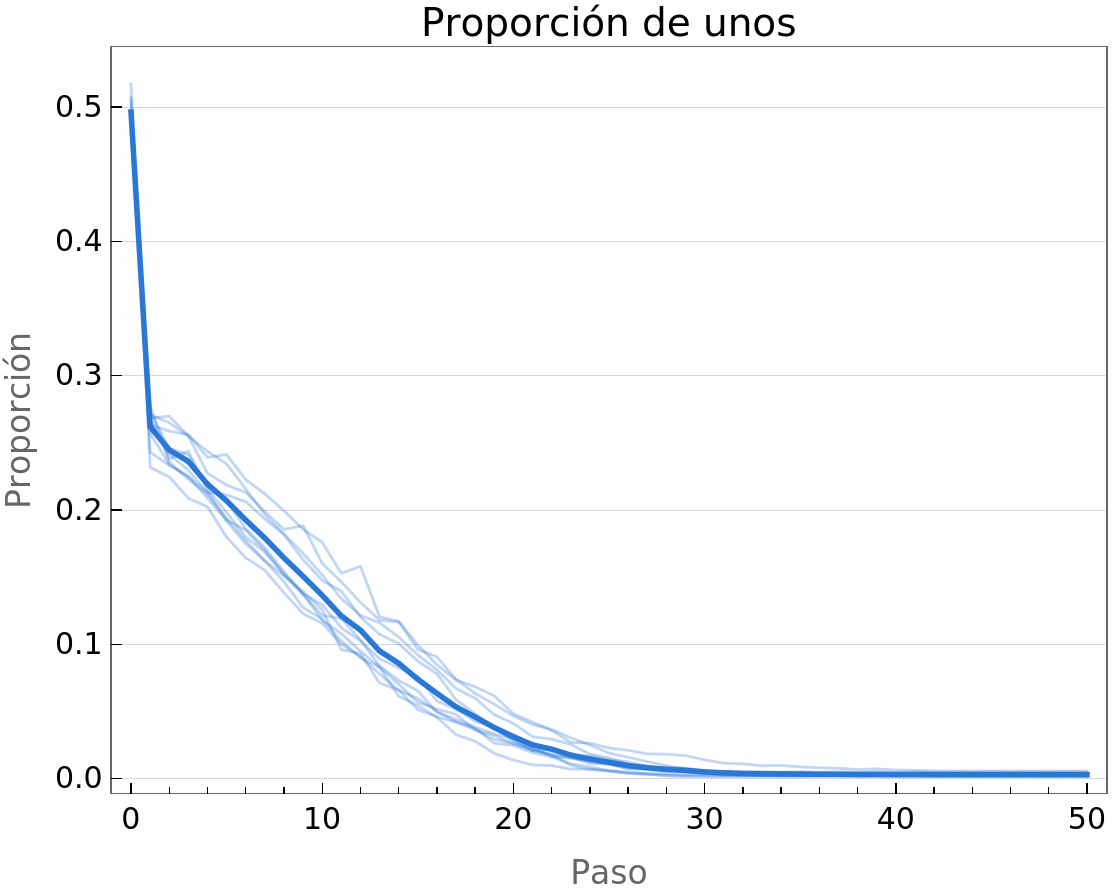
\includegraphics[width=0.77\linewidth]{img/experimentacion/duplicacion/gol/b3s23_reduction_1s.png}
		\caption{Proporción de unos en cada paso evolutivo.}
		\label{fig:b3s23_reduction_1s} 
	\end{subfigure}%
	\hfill % Añade espacio horizontal flexible entre las figuras
	\begin{subfigure}[b]{0.5\textwidth}
		\centering
		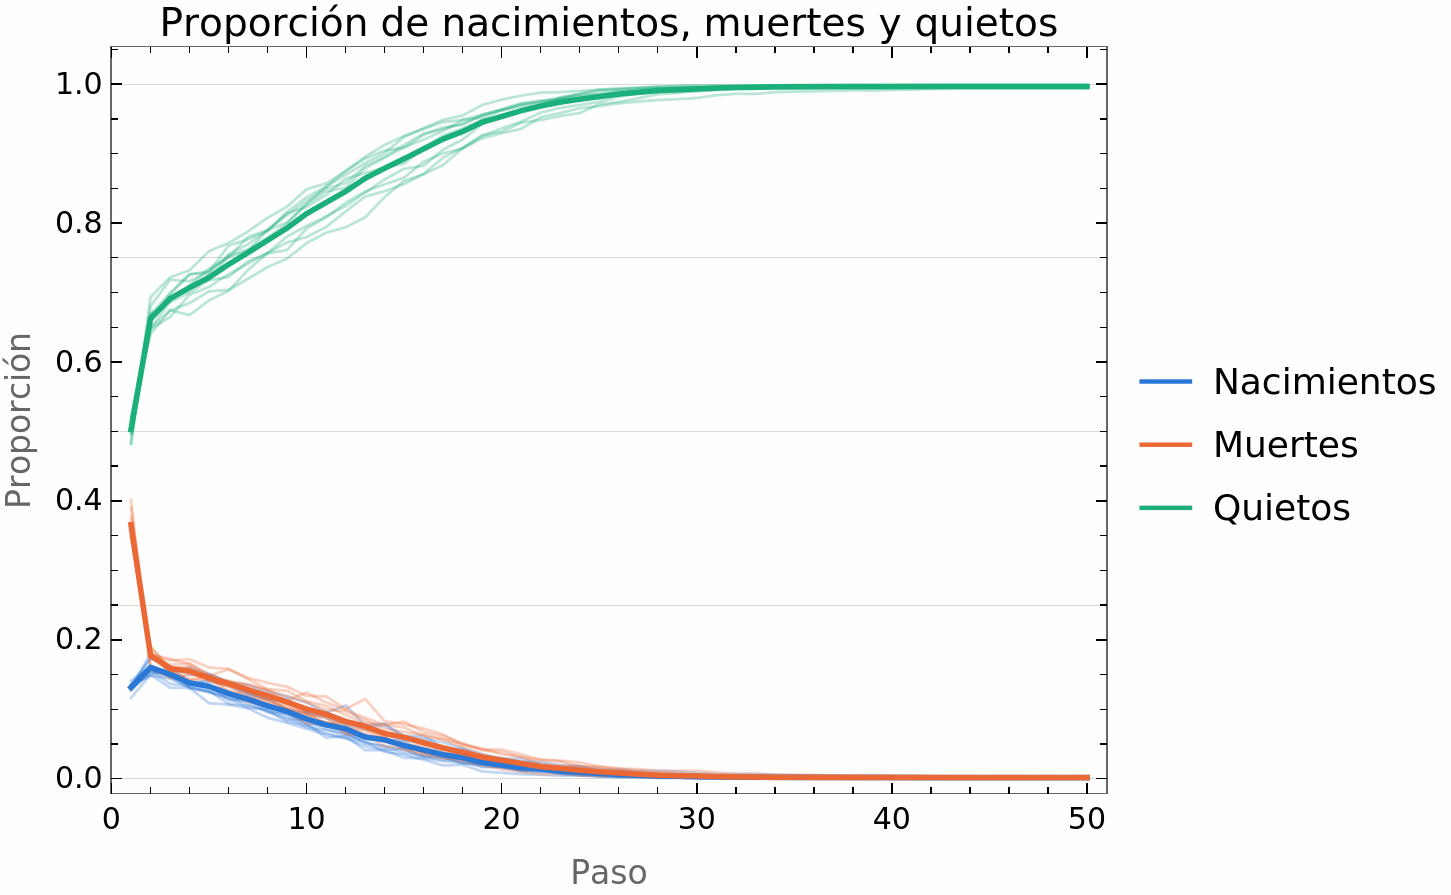
\includegraphics[width=\linewidth]{img/experimentacion/duplicacion/gol/b3s23_reduction_changes.png}
		\caption{Porcentaje de nacimientos, muertes y células sin cambios en cada paso evolutivo.}
		\label{fig:b3s23_reduction_changes}
	\end{subfigure}
	\caption{Proporciones de estados y cambios de estados en 10 evoluciones con condiciones iniciales aleatorias durante 50 pasos con el autómata celular neuronal obtenido por 16:16:ReLU \& 1:Sigmoid.}
	\label{fig:b3s23_c0n8}
\end{figure}

Por otro lado, el incremento de la vecindad no afecta la replicación del comportamiento. La red neuronal puede aprender la regla incluso con exceso de información. En la tabla \ref{tab:vecindad_ampliada} se muestran los mejores resultados con sus respectivas pérdidas finales; todas alcanzaron la pérdida objetivo en 21 épocas o menos.

\begin{table}[H]
	\centering
	\footnotesize
	\begin{tabular}{lllr}
		\toprule
		\textbf{Vecindad} & \textbf{Capa Oculta} & \textbf{Capa Salida} & \textbf{Pérdida} \\
		\midrule
		\multirow{3}{*}{$5\times5$} & 4:16:ReLU & 2:Linear & 0.000035 \\
		& 8:16:ReLU & 2:Linear & 0.000062 \\
		& 16:16:ReLU & 1:Sigmoid & 0.000225 \\
		\midrule
		\multirow{3}{*}{$7\times7$} & 8:16:ReLU & 2:Linear & 0.000023 \\
		& 8:16:ReLU & 1:Sigmoid & 0.000045 \\
		& 4:16:ReLU & 1:Sigmoid & 0.000137 \\
		\midrule
		\multirow{3}{*}{$8\times8$} & 8:16:ReLU & 2:Linear & 0.000063 \\
		& 8:16:ReLU & 1:Sigmoid & 0.000141 \\
		& 16:16:ReLU & 1:Sigmoid & 0.000156 \\
		\bottomrule
	\end{tabular}
	\caption{Las tres configuraciones con menor pérdida de la regla B3/S23 al aumentar la vecindad. Pérdida objetivo 0.001, límite de épocas: 500, tamaño del lote: 4,096, tasa de aprendizaje: 0.001, semilla aleatoria: 42. La vecindad de $8\times8$ abarca los desplazamientos $-4$ a $3$ en cada eje.}
	\label{tab:vecindad_ampliada}
\end{table}

Para finalizar, se realiza la sustitución, es decir, se elimina un elemento de la vecindad, pero se compensa con un incremento de vecinos circundantes en ese punto faltante. Esto se hace con el objetivo de analizar si la información adicional es útil o es únicamente ruido.

En la tabla \ref{tab:vecindad_reducida_ampliada} se experimenta con vecindades de $7 \times 7$ y $9 \times 9$ ignorando en cada caso un vecino: la esquina noroeste $(-1,-1)$ o el centro $(0,0)$. Se aprecia que el incremento de la vecindad reduce parcialmente la pérdida. Para el centro, pasamos de un 0.078650 a un 0.065987, y para el borde de 0.121294 a 0.097587.

\begin{table}[H]
	\centering
	\footnotesize
	\begin{tabular}{lllr}
		\toprule
		\textbf{Vecindad} & \textbf{Capa Oculta} & \textbf{Capa Salida} & \textbf{Pérdida} \\
		\midrule
		\multirow{4}{*}{$7\times7$ sin $(-1,-1)$} & 16:16:ReLU & 2:Linear & 0.099847 \\
		& 16:16:TanH & 1:Sigmoid & 0.098628 \\
		& 16:16:TanH & 2:Linear & 0.098407 \\
		& 16:16:ReLU & 1:Sigmoid & 0.099326 \\
		\midrule
		\multirow{4}{*}{$9\times9$ sin $(-1,-1)$} & 16:16:ReLU & 2:Linear & 0.098381 \\
		& 16:16:TanH & 1:Sigmoid & 0.097587 \\
		& 16:16:TanH & 2:Linear & 0.098029 \\
		& 16:16:ReLU & 1:Sigmoid & 0.098368 \\
		\midrule
		\multirow{4}{*}{$7\times7$ sin $(0,0)$} & 16:16:ReLU & 2:Linear & 0.067663 \\
		& 16:16:TanH & 1:Sigmoid & 0.066962 \\
		& 16:16:TanH & 2:Linear & 0.066976 \\
		& 16:16:ReLU & 1:Sigmoid & 0.068002 \\
		\midrule
		\multirow{4}{*}{$9\times9$ sin $(0,0)$} & 16:16:ReLU & 2:Linear & 0.067066 \\
		& 16:16:TanH & 1:Sigmoid & 0.066031 \\
		& 16:16:TanH & 2:Linear & 0.065987 \\
		& 16:16:ReLU & 1:Sigmoid & 0.067197 \\
		\bottomrule
	\end{tabular}
	\caption{Regla B3/S23 con vecindades de $7\times7$ y $9\times9$ sin un vecino. Pérdida objetivo 0.001, límite de épocas: 500, tamaño del lote: 4,096, tasa de aprendizaje: 0.001, semilla aleatoria: 42.}
	\label{tab:vecindad_reducida_ampliada}
\end{table}

Con estos resultados experimentales, establecemos algunas consideraciones esenciales para el entrenamiento de autómatas celulares neuronales:

\begin{itemize}
	\item La capacidad de generalización depende de clases y entradas balanceadas. Establecer una pérdida objetivo restrictiva fuerza a la red a ajustar sus pesos en regiones con patrones menos representados. El caso contrario atenúa estados y los conduce a otros comportamientos. 
	
	\item El entrenamiento de reglas semitotalísticas no garantiza que la regla aprendida también lo sea. 

	\item Incrementar el tamaño de la vecindad es un costo computacional viable cuando se desconoce el tamaño de la vecindad real. De igual manera, el incremento puede ayudar a disminuir la pérdida si aún existen vecinos que no fueron considerados, aunque con un límite contextual.

\end{itemize}

Estos experimentos confirman que no se requieren arquitecturas neuronales complejas para replicar este tipo de dinámicas evolutivas. Asimismo, queda validada la metodología propuesta para extraer e identificar el vector de regla aprendido por el modelo, sentando las bases para los siguientes experimentos del capítulo.

	\section{Pila de arena de Bak–Tang–Wiesenfeld}\label{sec:exp1_sandpile}

El siguiente experimento tiene el objetivo de replicar el comportamiento del sistema autoorganizado llamado \textit{sandpile} \cite{bak1987}. Es un sistema bidimensional que agrega granos de arena a una célula que, cuando alcanza un umbral, pierde sus granos y los distribuye en sus vecinos.

En un sentido estricto, el modelo de \textit{sandpile} no es un autómata celular, porque el sistema recibe constantemente una entrada (el grano de arena en el centro) que depende de la salida del sistema (cuando está en equilibrio). 

Para representar este sistema mediante un autómata celular se agrega un nuevo subconjunto de estados que representan el flujo constante de arena en cada paso evolutivo, salvo cuando la célula generadora se derrumba. 

Sea $\mathcal{S}_b = \{0,1,2,3,4, 5, 6, 7\}$ el conjunto de estados que definen la altura y sea $\mathcal{S}_i = \{ 0_i, 1_i, 2_i, 3_i, 4_i, 5_i, 6_i, 7_i, 8_i\}$ el conjunto de estados que definen la altura y que añaden granos; definimos entonces $\mathcal{S} = \mathcal{S}_b \cup \mathcal{S}_i$ como el conjunto completo de estados. 

Aunque el umbral de dispersión es de cuatro granos, se definen ocho alturas (de 0 a 7) para incluir todos los escenarios posibles. Por ejemplo: 
\[
\left[\begin{matrix}
	0 & 4 & 0 \\
	4 & 3 & 4 \\
	0 & 4 & 0
\end{matrix}\right] \rightarrow
\left[\begin{matrix}
	2 & 0 & 2 \\
	0 & 7 & 0 \\
	2 & 0 & 2
\end{matrix}\right] \rightarrow
\left[\begin{matrix}
	2 & 1 & 2 \\
	1 & 3 & 1 \\
	2 & 1 & 2
\end{matrix}\right]
\]
Del mismo modo, los estados generadores incluyen un estado adicional. Derivado del ejemplo anterior, si una célula generadora recibe el máximo de granos de sus vecinos, en el mismo paso recibe además su propio grano, lo que causa una nueva dispersión. Cuando la célula generadora se derrumba, no agrega su grano:
\[
\left[\begin{matrix}
	0 & 4 & 0 \\
	4 & 3_i & 4 \\
	0 & 4 & 0
\end{matrix}\right] \rightarrow
\left[\begin{matrix}
	2 & 0 & 2 \\
	0 & 8_i & 0 \\
	2 & 0 & 2
\end{matrix}\right] \rightarrow
\left[\begin{matrix}
	2 & 1 & 2 \\
	1 & 4_i & 1 \\
	2 & 1 & 2
\end{matrix}\right] \rightarrow
\left[\begin{matrix}
	2 & 2 & 2 \\
	2 & 0_i & 2 \\
	2 & 2 & 2
\end{matrix}\right]
\]

Existen $|\mathcal{S}| = 17$ estados y una vecindad de von Neumann (el centro y sus 4 vecinos). El vector de regla tiene un tamaño de $17^5 = 1{,}419{,}857$, y la regla del autómata celular que replica \textit{sandpile} es una entre $17^{1419857}$ posibles reglas. Su orden de complejidad es mucho mayor comparado con B3/S23. Es por esto que el objetivo del autómata celular neuronal será descifrar la regla que imite este comportamiento.

Con esta definición propuesta, fueron generadas 100 condiciones aleatorias con cuatro generadores en un espacio de $50 \times 50$ durante 1,500 pasos. 

De acuerdo con la figura \ref{fig:sp_proportion}, existen estados, como $8_i$, que tienen una probabilidad de aparición muy baja. Sin embargo, esta probabilidad se debe a que solo se consideran cuatro de 2,500 células. 

Por otro lado, si consideramos la evolución tradicional con el espacio vacío, con una única célula generadora, obtenemos las proporciones de la figura \ref{fig:sp_0_proportion}, donde aún existe la presencia de todos los estados, pero con una diferente dispersión. Cabe recordar que esta es la probabilidad de aparición de los estados y no la probabilidad de aparición de los patrones.

\begin{figure}[htbp!]
	\centering
	\begin{subfigure}[b]{0.45\textwidth}
		\centering
		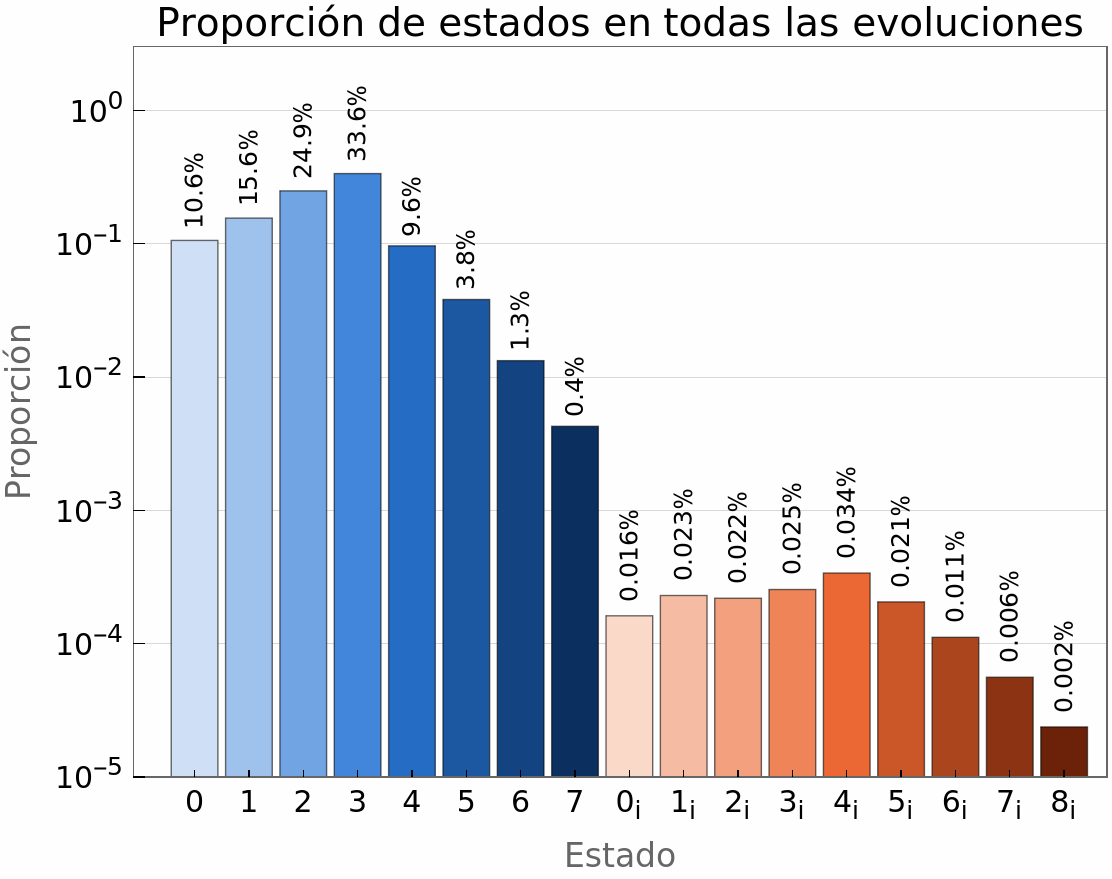
\includegraphics[width=\linewidth]{img/experimentacion/duplicacion/sandpile/sp_proportion.png}
		\caption{Distribuciones de probabilidad con múltiples condiciones iniciales.}
		\label{fig:sp_proportion}
	\end{subfigure}
	\hfill % Añade espacio horizontal flexible entre las figuras
	\begin{subfigure}[b]{0.45\textwidth}
		\centering
		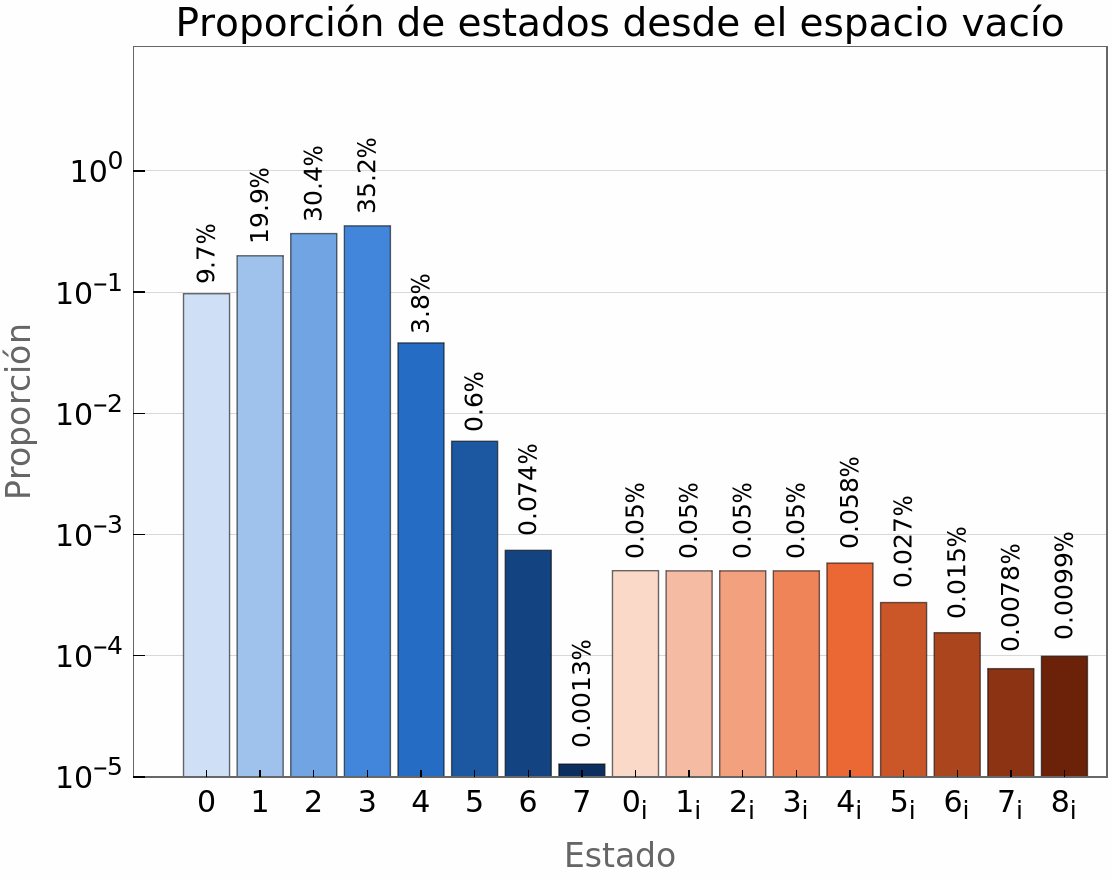
\includegraphics[width=\linewidth]{img/experimentacion/duplicacion/sandpile/sp_0_proportion.png}
		\caption{Distribuciones de probabilidad con un único generador.}
		\label{fig:sp_0_proportion}
	\end{subfigure}
	\caption{Distribución de probabilidad de aparición de todos los estados en la regla \textit{sandpile}. Azul para los estados normales y naranja para los generadores. }
	\label{fig:sp_proporciones}
\end{figure}

\subsection{Capacidad de replicación}

En la tabla \ref{tab:sp_activaciones} se muestran 5 diferentes pruebas para encontrar la mejor combinación de funciones de activación. Se entrenó con un único generador en el centro y la combinación 16:16:ReLU \& 17:Linear fue la que dio mejores resultados, con una pérdida de 0.009935 durante 500 épocas. 

\begin{table}[H]
	\centering
	\footnotesize
	\begin{tabular}{llrrr}
		\toprule
		\textbf{Capa Oculta} & \textbf{Capa Salida} & \textbf{Pérdida} & \textbf{Exactitud (\%)} & \textbf{\shortstack{Exactitud\\generador (\%)}} \\
		\midrule
		16:16:ReLU & \multirow{3}{*}{17:Linear} & 0.009935 & 99.417 & 91.600 \\
		16:16:Sigmoid & & 1.252780 & 55.318 & 0.000 \\
		16:16:TanH & & 0.011293 & 99.604 & 58.350 \\
		\midrule
		\multirow{3}{*}{16:16:ReLU} & 17:Linear & 0.009935 & 99.417 & 91.600 \\
		 & 17:Sigmoid & 2.200967 & 55.318 & 0.000 \\
		 & 17:TanH & 1.754721 & 55.318 & 0.000 \\
		\bottomrule
	\end{tabular}
	\caption{Regla \textit{sandpile} con múltiples funciones de activación en la capa oculta y en la capa de salida: pérdida objetivo 0.001, límite de épocas: 500, tamaño del lote: 4,096, tasa de aprendizaje: 0.0003, semilla aleatoria: 42.}
	\label{tab:sp_activaciones}
\end{table}

Posteriormente, fue probada la mejor combinación de funciones de activación (ReLU y Linear) con diferentes tamaños de red, tasas de aprendizaje y pérdidas objetivo (ver tabla \ref{tab:sp_arquitecturas}). Incrementar el número de capas no proporciona mejores resultados; en su lugar, es preferible el uso de más neuronas por capa. La tasa de aprendizaje de 0.001 es la que da mejores resultados, y con ella se reproduce el 100\% de los datos de entrenamiento si se configura la red neuronal con 2:64:ReLU \& 17:Linear.  

\begin{table}[H]
	\centering
	\footnotesize
	\setlength{\tabcolsep}{4pt}
	\begin{tabular}{lrrrrrr}
		\toprule
		\textbf{Capa Oculta} & \textbf{\shortstack{Tasa de\\aprendizaje}} & \textbf{\shortstack{Pérdida\\objetivo}} & \textbf{Épocas} & \textbf{Pérdida} & \textbf{\shortstack{Exactitud\\(\%)}} & \textbf{\shortstack{Exactitud\\generador (\%)}} \\
		\midrule
		16:16:ReLU & 0.0003 & 0.001 & 500 & 0.009935 & 99.417 & 91.600 \\
		\midrule
		\multirow{5}{*}{32:32:ReLU} & 0.003 & 0.001 & 500 & 0.709890 & 69.026 & 0.000 \\
		 & 0.001 & 0.001 & 500 & 0.012164 & 99.679 & 89.750 \\
		 & 0.0003 & 0.001 & 500 & 0.022682 & 99.234 & 50.850 \\
		 & 0.0001 & 0.001 & 500 & 0.025121 & 99.104 & 79.900 \\
		 & 0.00003 & 0.001 & 500 & 0.026755 & 99.207 & 69.150 \\
		\midrule
		\multirow{2}{*}{8:32:ReLU} & 0.001 & 0.001 & 202 & 0.000989 & 99.970 & 94.100 \\
		 & 0.001 & 0.0001 & 476 & 0.000093 & 99.996 & 100.000 \\
		\midrule
		8:16:ReLU & 0.001 & 0.0001 & 1,256 & 0.000086 & 99.998 & 99.950 \\
		4:32:ReLU & 0.001 & 0.0001 & 392 & 0.000098 & 99.998 & 100.000 \\
		2:64:ReLU & 0.001 & 0.0001 & 351 & 0.000099 & 99.999 & 100.000 \\
		2:32:ReLU & 0.001 & 0.0001 & 1,333 & 0.000079 & 99.999 & 100.000 \\
		 2:64:ReLU & 0.001 & 0.00001 & 630 & 0.000010 & 100.000 & 100.000 \\
		\bottomrule
	\end{tabular}
	\caption{Regla \textit{sandpile} con capa de salida 17:Linear y distintos tamaños de red. Tasa de aprendizaje constante, límite de épocas: 500 en 16:16:ReLU y 32:32:ReLU, tamaño del lote: 4,096, semilla aleatoria: 42.}
	\label{tab:sp_arquitecturas}
\end{table}

Los datos de entrenamiento pudieron haber tenido condiciones iniciales aleatorias, pero en este experimento se busca acercarse más al escenario en donde no se conoce la regla, por lo que se experimenta sin la posibilidad de generar todos los escenarios ideales que favorezcan la replicación del comportamiento. De esta forma, queda demostrado que el autómata celular neuronal puede aprender el comportamiento de \textit{sandpile} una vez que se representa como un autómata celular. La figura \ref{fig:sp_nca} muestra la misma configuración en el paso 1,000 entre \textit{sandpile} y el autómata celular neuronal.

\begin{figure}[htbp!]
	\centering
	\begin{subfigure}[b]{0.5\textwidth}
		\centering
		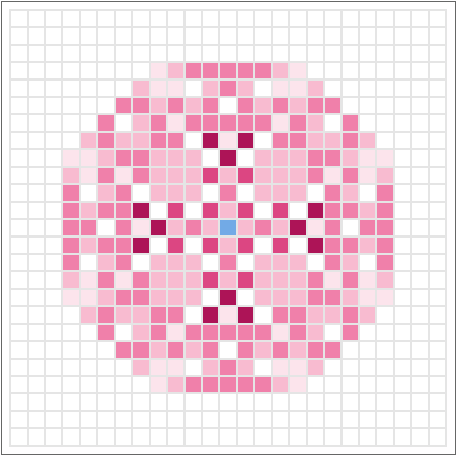
\includegraphics[width=0.65\linewidth]{img/experimentacion/duplicacion/sandpile/sp_1000.png}
		\caption{Evolución de \textit{sandpile} original generada en Mathematica.}
		\label{fig:sp_1000} 
	\end{subfigure}%
	\hfill % Añade espacio horizontal flexible entre las figuras
	\begin{subfigure}[b]{0.5\textwidth}
		\centering
		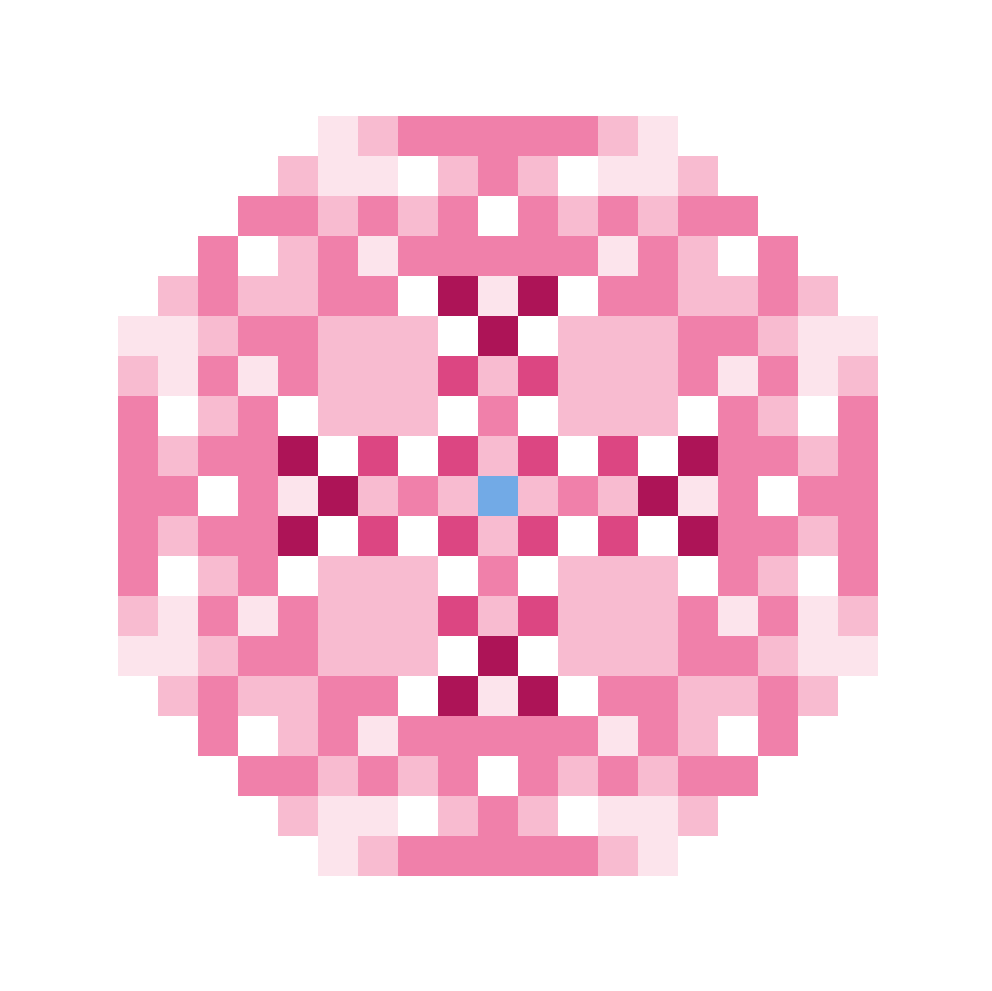
\includegraphics[width=0.6\linewidth]{img/experimentacion/duplicacion/sandpile/sp_nca_1000.png}
		\caption{Evolución del autómata celular neuronal originada en el simulador.}
		\label{fig:sp_nca_1000}
	\end{subfigure}
	\caption{Comparativa de simulaciones entre el sistema original (figura \ref{fig:sp_1000}) y la regla aprendida (figura \ref{fig:sp_nca_1000}). Células generadoras en tonos azules. }
	\label{fig:sp_nca}
\end{figure}

\subsection{Reducción de la tasa de aprendizaje}

El autómata celular neuronal pudo replicar el comportamiento exacto de la evolución con la que fue entrenado: una única célula generadora en el centro. Sin embargo, esa configuración no fue capaz de generalizar el comportamiento. Esto se observa cuando existen múltiples células generadoras, lo que causa la generación de más de ellas o la eliminación de las mismas (ver figura \ref{fig:sp_nca_err_1}).

\begin{figure}[htbp]
	\centering
	\begin{subfigure}[b]{0.45\textwidth}
		\centering
		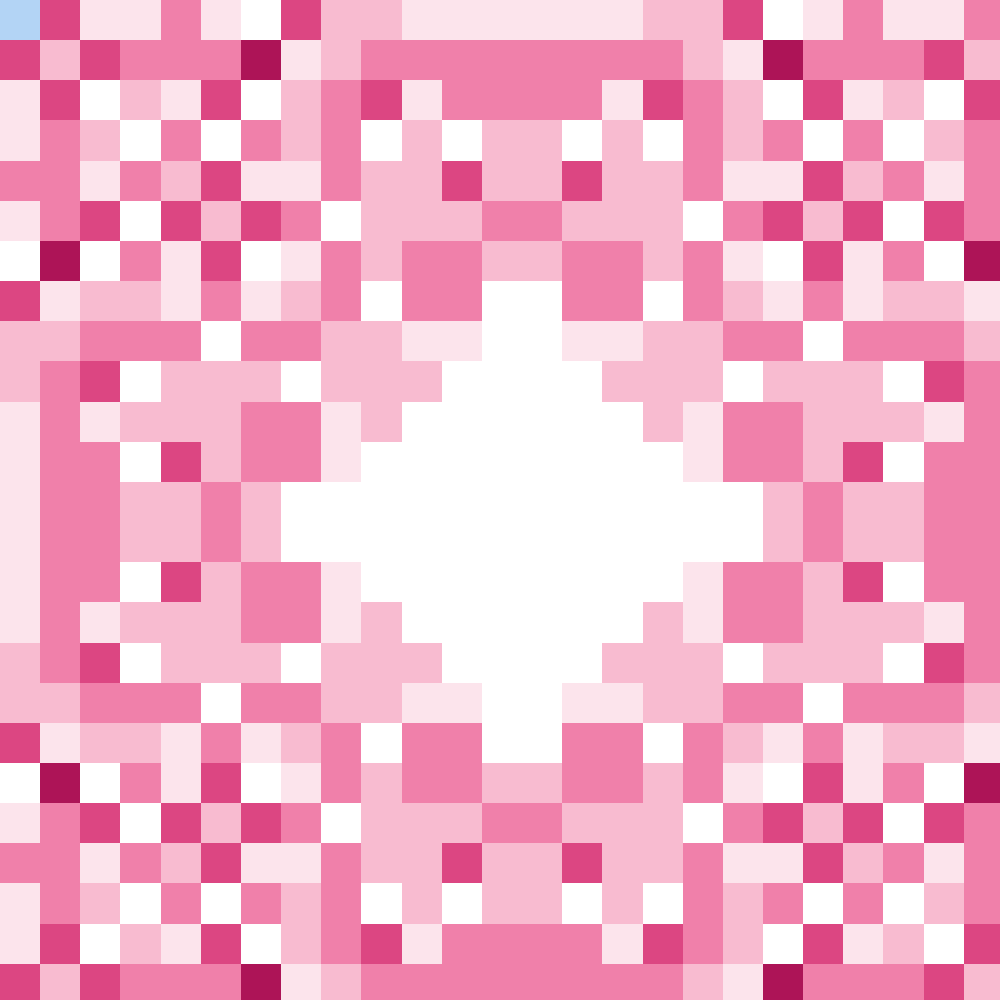
\includegraphics[width=0.45\linewidth]{img/experimentacion/duplicacion/sandpile/sp_nca_step_1928.png}
		\caption{Evolución en el paso 1,928.}
		\label{fig:sp_nca_step_1928} 
	\end{subfigure}%
	\hfill % Añade espacio horizontal flexible entre las figuras
	\begin{subfigure}[b]{0.45\textwidth}
		\centering
		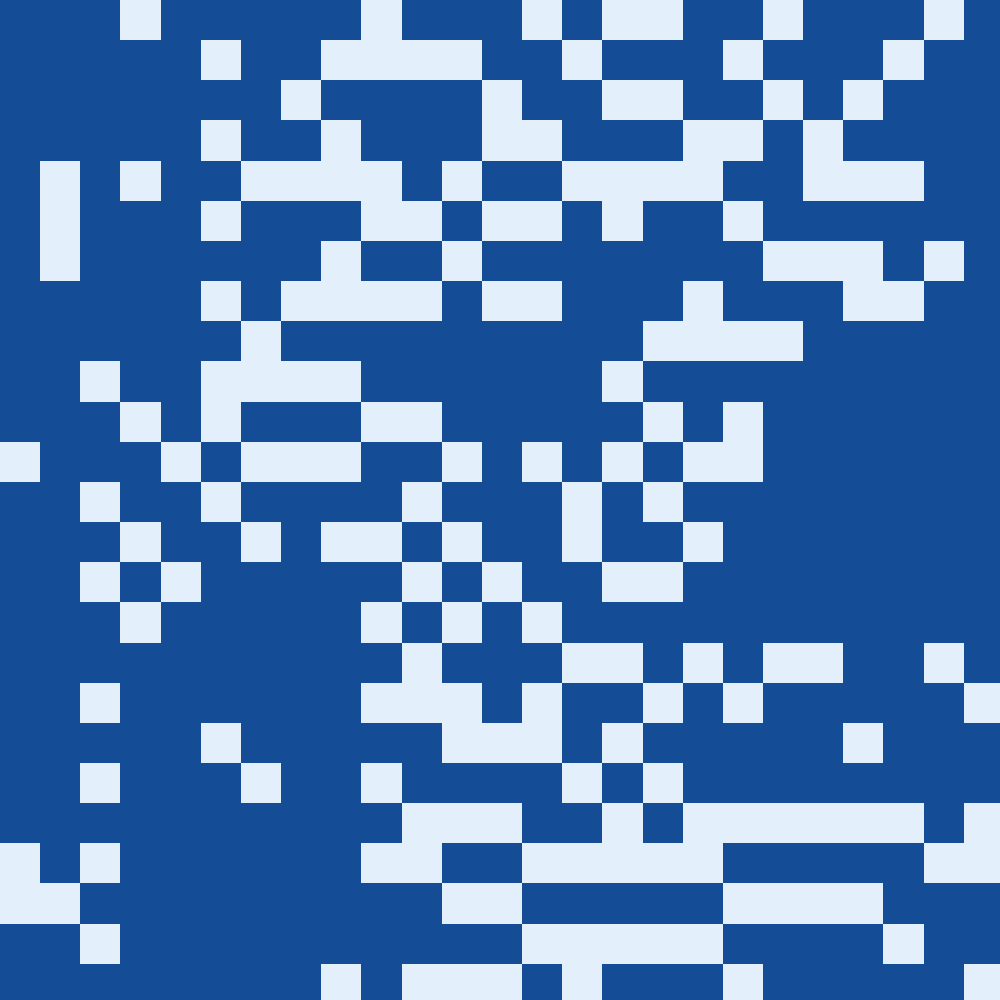
\includegraphics[width=0.5\linewidth]{img/experimentacion/duplicacion/sandpile/sp_nca_step_2080.png}
		\caption{Evolución en el paso 2,080.}
		\label{fig:sp_nca_step_2080}
	\end{subfigure}

	\vspace{1em}
	\begin{subfigure}[b]{0.45\textwidth}
		\centering
		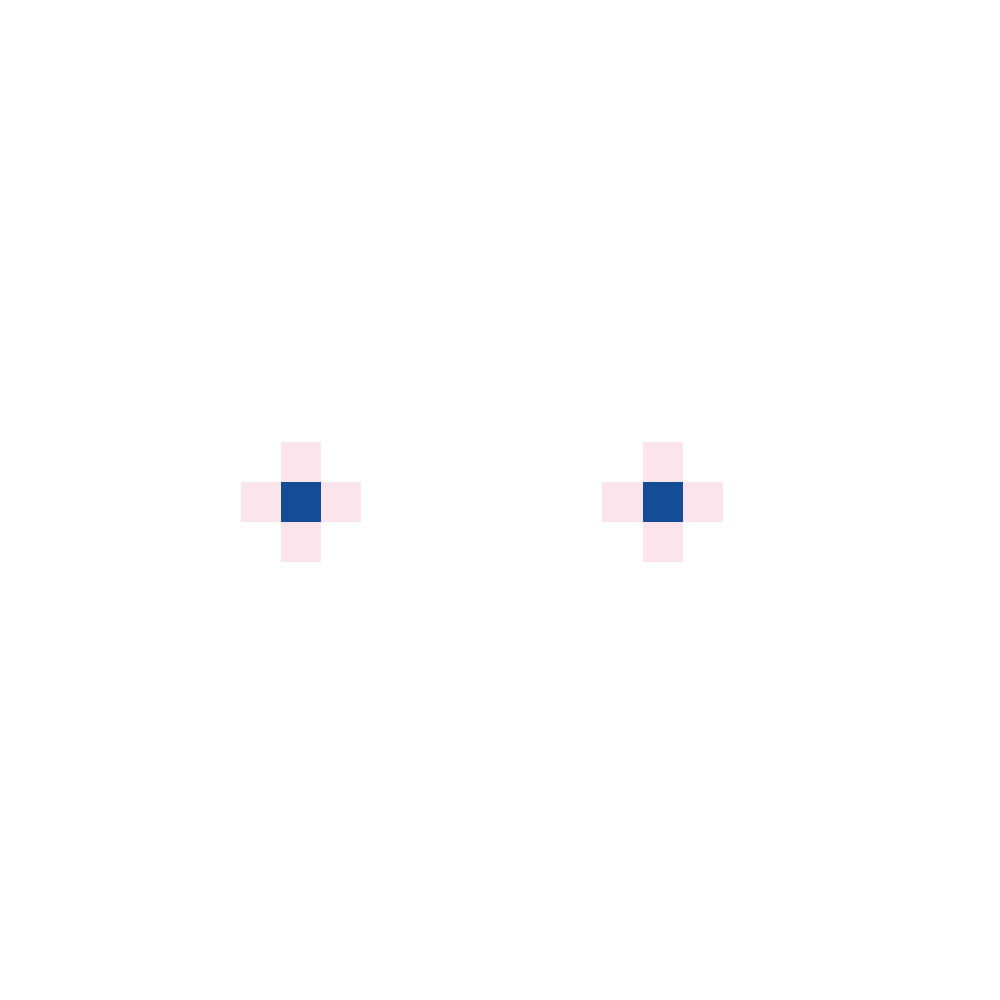
\includegraphics[width=0.45\linewidth]{img/experimentacion/duplicacion/sandpile/sp_nca_2_step_9.png}
		\caption{Evolución en el paso 9.}
		\label{fig:sp_nca_2_step_9} 
	\end{subfigure}
	\hfill 
	\begin{subfigure}[b]{0.45\textwidth}
		\centering
		
\includegraphics[width=0.45\linewidth]{img/experimentacion/duplicacion/sandpile/sp_nca_2_step_246.png}
		\caption{Evolución en el paso 246.}
		\label{fig:sp_nca_2_step_246}
	\end{subfigure}
	\caption{Célula generadora en $(0, 0)$ con frontera periódica (figuras \ref{fig:sp_nca_step_1928} y \ref{fig:sp_nca_step_2080}) y dos células generadoras separadas por ocho células (figuras \ref{fig:sp_nca_2_step_9} y \ref{fig:sp_nca_2_step_246}).}
	\label{fig:sp_nca_err_1}
\end{figure}


Además, la red fue entrenada con datos de frontera abierta, donde la arena que cae fuera de los bordes desaparece. Por esta razón el sistema no puede replicar el escenario en donde la arena llena el espacio. En la figura \ref{fig:sp_nca_step_2080} las generadoras se propagan cuando hay mucha arena en el sistema. El mismo efecto ocurre cuando existen generadoras muy juntas. 

Para solucionar el problema de la eliminación de células generadoras, se entrena con dos evoluciones en un espacio de $25 \times 25$ y 2,000 pasos cada una: la primera con una célula generadora y la segunda con cuatro células generadoras. Este nuevo experimento permite que coexistan varias (sin tocarse), pero revela un comportamiento oscilatorio en la pérdida de la red neuronal. De acuerdo con la figura \ref{fig:sp_4generadores_loss}, esta decrece de forma limpia hasta cerca de 150 épocas y continúa de forma errática. 

\begin{figure}[H]
	\centering
	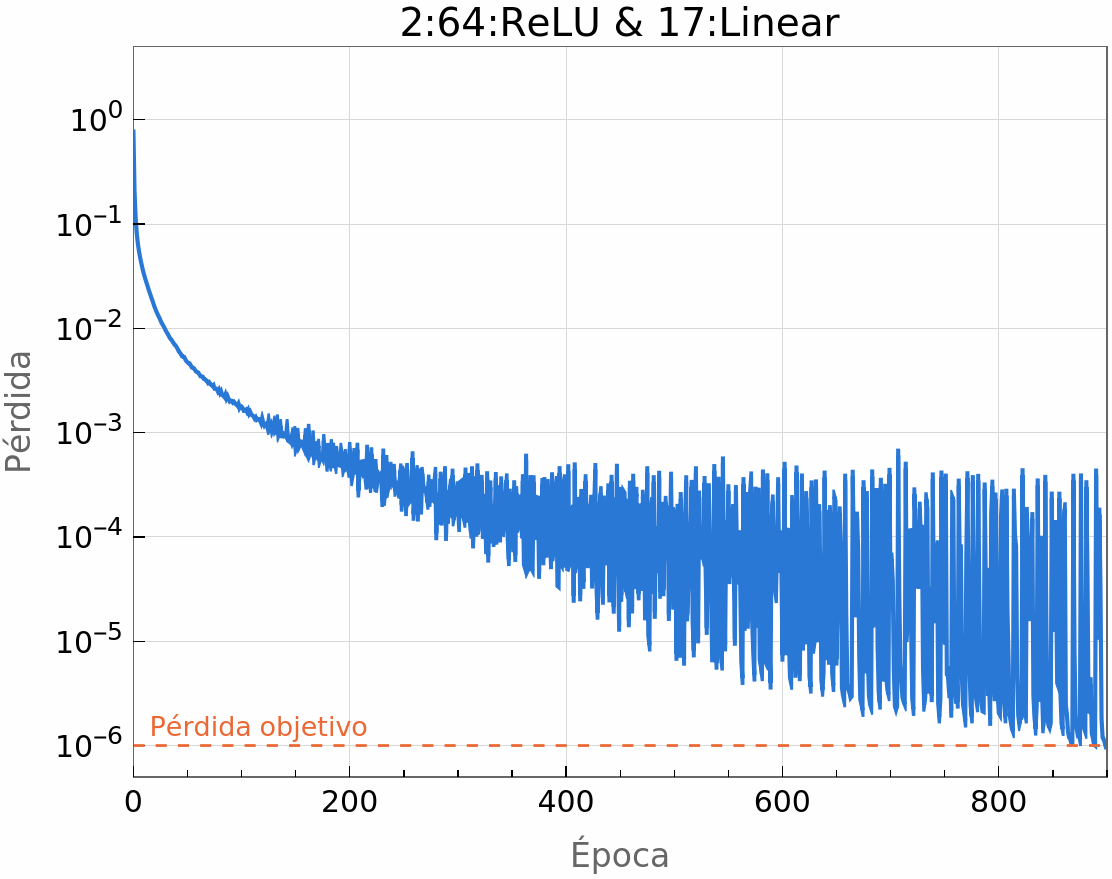
\includegraphics[width=0.5\linewidth]{img/experimentacion/duplicacion/sandpile/sp_4generadores_loss.png}
	\caption{Pérdida de la red neuronal al entrenar \textit{sandpile} con 4 generadores, tasa de aprendizaje constante de 0.001 y pérdida objetivo de 0.000001.}
	\label{fig:sp_4generadores_loss}
\end{figure}


Se proponen dos soluciones: reducción exponencial y reducción dinámica de la tasa de aprendizaje:

\begin{itemize}
	\item La reducción exponencial calcula la tasa de aprendizaje de la siguiente forma:	
	\[
	\mathrm{lr}(e) = \mathrm{lr}_{0} \left( \frac{\mathrm{lr}_{\min}}{\mathrm{lr}_{0}} \right)^{\frac{e}{E - 1}}
	\]
	donde $\mathrm{lr}_{0} = 0.001$ es la tasa inicial, $\mathrm{lr}_{\min} = 0.000001$ la tasa final, $e = 0,1, \dots, E - 1$ es la época actual y $E = 2{,}000$ es el total de épocas.
	Aunque su curva está más suavizada, la tasa le impide alcanzar la pérdida objetivo y terminó por límite de épocas con una pérdida de 0.000015 (ver figura \ref{fig:sp_4generadores_loss_exp}).
	
	\item La reducción dinámica o de \textit{plateau} divide la tasa a la mitad cada vez que la pérdida se estanca mediante la siguiente fórmula:
	\[
	\mathrm{lr}(e) = \max\left( \mathrm{lr}_{0} \cdot f^{n(e)},\ \mathrm{lr}_{\min} \right)
	\]
	donde $f = 0.5$ es el factor de reducción y $n(e)$ es el número de veces que la pérdida dejó de mejorar durante $p = 20$ épocas seguidas antes de la época $e$. Con esta reducción se alcanza la pérdida objetivo, pero en 1,319 épocas (figura \ref{fig:sp_4generadores_loss_plateau}).
\end{itemize}

\begin{figure}[htbp]
	\centering
	\begin{subfigure}[b]{0.45\textwidth}
		\centering
		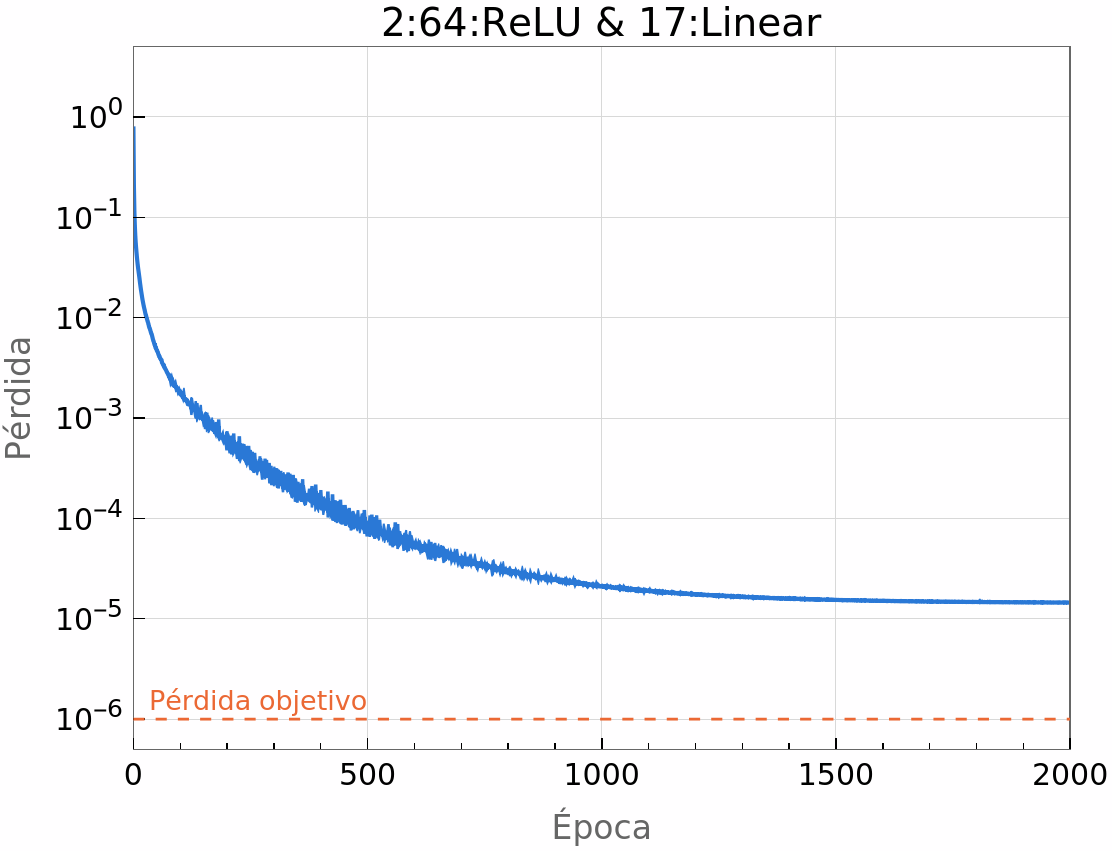
\includegraphics[width=\linewidth]{img/experimentacion/duplicacion/sandpile/sp_4generadores_loss_exp.png}
		\caption{Decrecimiento de la tasa de aprendizaje mediante reducción exponencial.}
		\label{fig:sp_4generadores_loss_exp}
	\end{subfigure}
	\hfill 
		\begin{subfigure}[b]{0.45\textwidth}
		\centering
		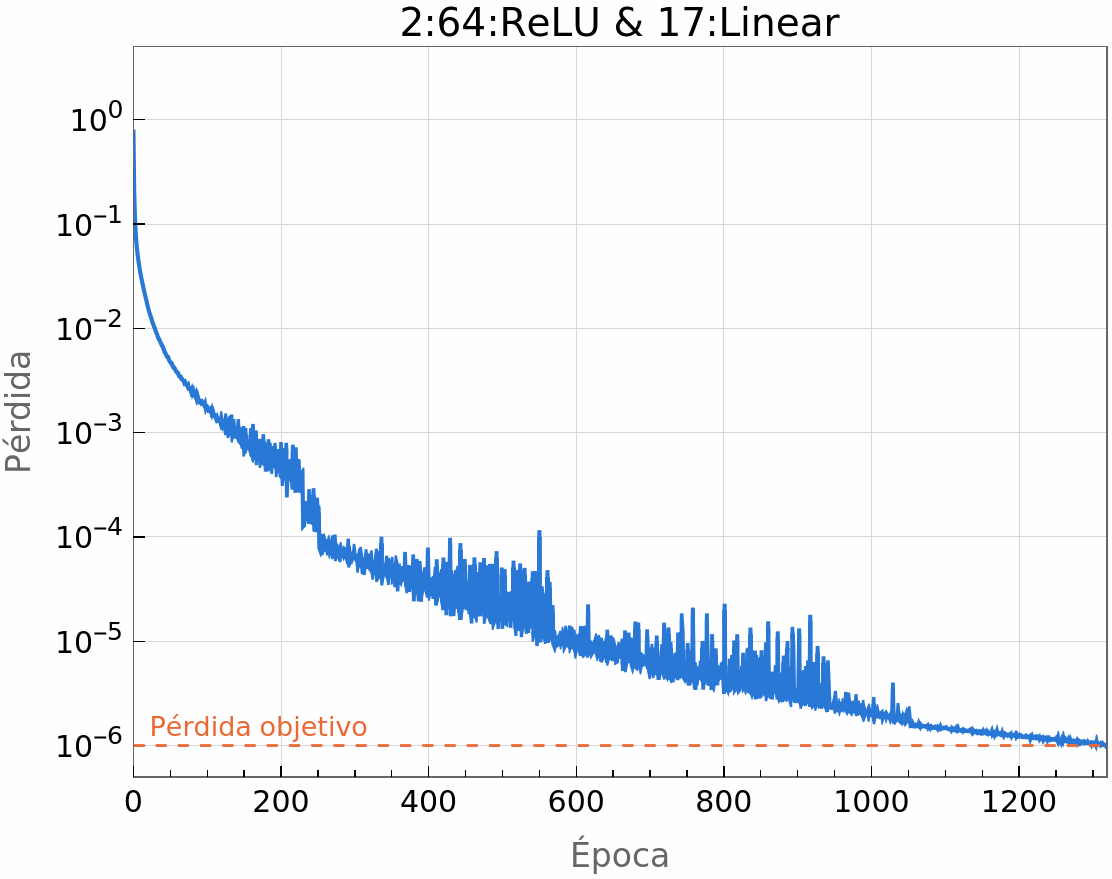
\includegraphics[width=\linewidth]{img/experimentacion/duplicacion/sandpile/sp_4generadores_loss_plateau.png}
		\caption{Decrecimiento de la tasa de aprendizaje mediante reducción por \textit{plateau}.}
		\label{fig:sp_4generadores_loss_plateau}
	\end{subfigure}
	\caption{Pérdida de la red neuronal al entrenar \textit{sandpile} con cuatro generadores y una pérdida objetivo de 0.000001 con las técnicas de reducción de tasa de aprendizaje exponencial (figura \ref{fig:sp_4generadores_loss_exp}) y dinámica (figura \ref{fig:sp_4generadores_loss_plateau}). }
	\label{fig:sp_4generadores_loss_red}
\end{figure}

Todas fueron entrenadas con una pérdida objetivo exigente (0.000001) y tuvieron una exactitud del 100\%. Cabe recordar que la exactitud mide cuántas predicciones fueron correctas y la pérdida, la seguridad de dicha decisión. Además, al evolucionar un generador en el centro de un espacio de $25 \times 25$ con frontera abierta, las tres rompen la simetría: la reducción exponencial en el paso 2,615, el resto en el 3,241. Solo la reducción dinámica genera un segundo generador, en el paso 4,045, y llena casi todo el espacio con generadores (85\%) en el 4,266; las otras dos no generan generadores adicionales en 6,000 pasos.

\subsection{Capa de entrada con \textit{one-hot encoding}}

La capa de entrada de la red neuronal para B3/S23 consiste en nueve células, cada una con un valor de cero o uno. Sin embargo, en \textit{sandpile} existen solo cinco células, pero cada una de ellas puede adquirir uno de 17 valores. Esta falta de normalización dificulta la tarea de predicción. 

Una red neuronal es un proceso que combina números mediante funciones de agregación en cada neurona. Al tratar los datos de manera secuencial estamos indicando que existe la misma relación entre cada par de valores con la misma distancia. Para \textit{sandpile}, los estados del 0 al 7 corresponden a las alturas posibles de arena y los estados del 8 al 16 corresponden a las alturas de 0 a 8 para las generadoras. Sin embargo, al escoger una escala lineal estamos indicando que la relación que existe entre el estado 0 y el 1 o el 9 y el 10 es la misma que entre el 7 y el 8. Es por esto que Menchaca en \cite{MenchacaMendez2022} sugiere el uso de \textit{one-hot encoding}, una técnica de codificación de datos binaria.

En este caso, la capa de entrada pasa de tener 5 neuronas con valores entre 0 y 16 a $17 \times 5 = 85$ neuronas con valores de 0 o 1.

Al entrenar con un único generador (tabla \ref{tab:sp_onehot_1gen}), el autómata celular neuronal con \textit{one-hot} sobrevive 5,149 pasos antes de romper la simetría, 3,106 pasos más que sin \textit{one-hot} (2,043). Sin embargo, sigue siendo incapaz de evolucionar junto con otro generador.

\begin{table}[H]
	\centering
	\footnotesize
	\setlength{\tabcolsep}{4pt}
	\begin{tabular}{lrrrrr}
		\toprule
		\textbf{Entrada} & \textbf{Épocas} & \textbf{Pérdida} & \textbf{\shortstack{Tiempo\\(s)}} & \textbf{\shortstack{Exactitud\\(\%)}} & \textbf{\shortstack{Exactitud\\generador (\%)}} \\
		\midrule
		Sin \textit{one-hot} & 1,200 & 0.000003 & 140.97 & 100.000 & 100.000 \\
		\textit{One-hot} & 40 & 0.000001 & 4.92 & 100.000 & 100.000 \\
		\bottomrule
	\end{tabular}
	\caption{Regla \textit{sandpile} con un generador, con capas: 2:64:ReLU \& 17:Linear, pérdida objetivo 0.000001, límite de épocas: 1,200, tamaño del lote: 4,096, tasa de aprendizaje inicial: 0.001 con reducción \textit{plateau}, semilla aleatoria: 42. La red sin \textit{one-hot} terminó por límite de épocas.}
	\label{tab:sp_onehot_1gen}
\end{table}

Por otro lado, en la tabla \ref{tab:sp_onehot} se entrena con cuatro generadores; utilizando \textit{one-hot}, converge en 63 veces menos épocas y 53 veces menos tiempo. Además, esta configuración sobrevive al menos 10,000 pasos en la configuración tradicional y 2,985 con frontera periódica antes de romper la simetría. 

\begin{table}[H]
	\centering
	\footnotesize
	\setlength{\tabcolsep}{4pt}
	\begin{tabular}{lrrrrr}
		\toprule
		\textbf{Entrada} & \textbf{Épocas} & \textbf{Pérdida} & \textbf{\shortstack{Tiempo\\(s)}} & \textbf{\shortstack{Exactitud\\(\%)}} & \textbf{\shortstack{Exactitud\\generador (\%)}} \\
		\midrule
		Sin \textit{one-hot} & 1,319 & 0.000001 & 301.47 & 100.000 & 100.000 \\
		\textit{One-hot} & 21 & 0.000001 & 5.67 & 100.000 & 100.000 \\
		\bottomrule
	\end{tabular}
	\caption{Regla \textit{sandpile} con un generador y con 4 generadores (dos evoluciones de $25\times25$ con 2,000 pasos), con capas: 2:64:ReLU \& 17:Linear, pérdida objetivo 0.000001, tamaño del lote: 4,096, tasa de aprendizaje inicial: 0.001 con reducción \textit{plateau}, semilla aleatoria: 42.}
	\label{tab:sp_onehot}
\end{table}

Adicionalmente, este nuevo autómata celular neuronal replicó parcialmente un comportamiento que nunca se le había presentado: dos generadores contiguos. Si iniciamos el sistema con dos generadores contiguos en el centro de un espacio de $25 \times 25$, ambas evoluciones coinciden durante 1,882 pasos y en el siguiente se rompe la similitud, tal como se muestra en la figura \ref{fig:sp_2gen}. El error ocurre en la célula generadora con 5 granos contigua a la otra generadora, un patrón que no aparece en los datos de entrenamiento. En espacios de $20 \times 20$ y $50 \times 50$ el primer error aparece en los pasos 1,270 y 6,265, respectivamente, y en $100 \times 100$ no hay errores en 10,000 pasos.

\begin{figure}[htbp]
	\centering
	\begin{subfigure}[b]{0.45\textwidth}
		\centering
		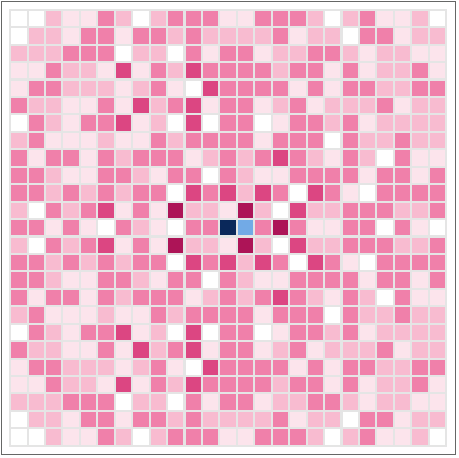
\includegraphics[width=0.7\linewidth]{img/experimentacion/duplicacion/sandpile/sp_2gen_step_1883.png}
		\caption{Evolución de \textit{sandpile} original generada en Mathematica.}
		\label{fig:sp_2gen_original}
	\end{subfigure}
	\hfill 
	\begin{subfigure}[b]{0.45\textwidth}
		\centering
		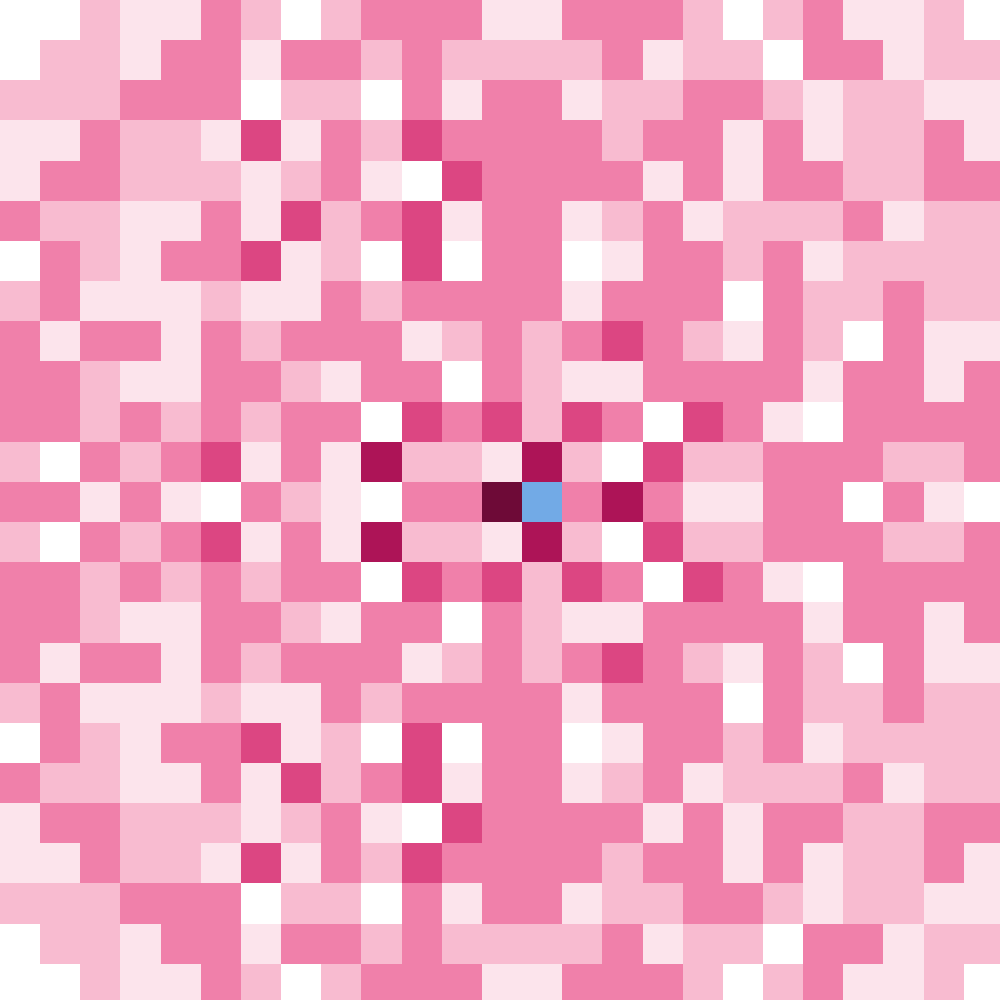
\includegraphics[width=0.67\linewidth]{img/experimentacion/duplicacion/sandpile/sp_nca_2gen_step_1883.png}
		\caption{Evolución del autómata celular neuronal originada en el simulador.}
		\label{fig:sp_2gen_nca}
	\end{subfigure}
	\caption{Comparativa de simulaciones entre el sistema original (figura \ref{fig:sp_2gen_original}) y la regla aprendida (figura \ref{fig:sp_2gen_nca}) con 2 células generadoras contiguas en el centro después de 1,883 pasos. }
	\label{fig:sp_2gen}
\end{figure}

La forma de representar \textit{sandpile} como un autómata celular nos permitió explorar y definir mejoras en la definición de la red neuronal. Aunque el sistema no pudo extrapolar el comportamiento con una célula generadora a múltiples, sí pudo generalizar parcialmente hacia generadoras contiguas. Este descubrimiento nos indica que la red neuronal se acerca al comportamiento de sumas que se presenta al derribar las torres, tanto para las células normales como para las generadoras, aunque sigue fallando en patrones que no aparecen en los datos de entrenamiento. Esto es gracias a la codificación \textit{one-hot}, que no crea relaciones lineales entre los datos, fenómeno que pasó desapercibido con dos estados en las reglas del juego de la vida, ya que era codificación binaria. 

	\subsection{Hormiga de Langton}

El último experimento de esta sección busca imitar el comportamiento de la hormiga de Langton, un agente reactivo que vive en un espacio bidimensional. Este sistema no fue concebido como un autómata celular en un sentido estricto, pero a diferencia de \textit{sandpile}, sí se puede definir como uno sin necesidad de manipular su comportamiento. 

Originalmente, la hormiga de Langton realiza un par de acciones según el estado de la célula que esté pisando, estas incluyen cambiar el color y cambiar de dirección. La representación mediante un autómata celular pone el foco en cada célula, donde la mayoría está en un estado de naturaleza muerta hasta que tienen un vecino que contiene una hormiga a punto de caminar encima de ella.

Para este experimento se considera la convención original en una cuadrícula, cada una con 2 estados y una hormiga con 2 instrucciones, girar a la derecha con blancos y a la izquierda con negros. Además, para representar la posición de la hormiga se requieren dos conjuntos de estados que incluyen las cuatro direcciones para blanco y negro. 

Es necesario considerar la dirección por cada color. Considerando la célula del centro en el siguiente escenario:
\[
\left[
\begin{matrix}
	0 & \downarrow & 0 \\
	0 & 0 & 0 \\
	0 & 0 & 0 
\end{matrix} \right] \rightarrow
\left[ \begin{matrix}
	0 & 0 & 0 \\
	0 & \leftarrow & 0 \\
	0 & 0& 0 \\
\end{matrix}  \right]\rightarrow
\left[ \begin{matrix}
0 & 0 & 0 \\
\uparrow & x & 0 \\
0 & 0& 0 \\
\end{matrix}  \right]
\]
En el primer paso, la información que recibe de sus vecinos y de sí misma es que una hormiga caminará sobre él y cambiará su dirección. En el siguiente paso, sabe que tiene que dejar de ser una hormiga y convertirse en un estado, pero el sistema no tiene memoria, es decir, no recuerda qué estado era antes de ser la dirección de la hormiga, por lo que pierde el contexto de la situación.

El vector de regla tiene un tamaño de $10^{5} = 100{,}000$, y la hormiga de Langton es una regla entre $10^{100000}$. Otra limitación de este sistema es la cantidad de información que presenta, pues los únicos cambios existen cuando una hormiga está cerca. Tratar a la hormiga como un autómata celular es computacionalmente más complejo, pero este experimento busca la extracción de sistemas con poca información. 

En un espacio de $100 \times 100$ si evolucionamos el sistema por 11,000 pasos con una configuración inicial vacía obtenemos la distribución de estados de la figura \ref{fig:langton_RL_100x100_proporcion}, donde se observa el problema de distribución de clases. Por otro lado, si consideramos múltiples condiciones iniciales aleatorias pero una única hormiga, obtenemos los datos de la figura \ref{fig:langton_RL_aleatorias_proporcion}, donde la única diferencia es la distribución entre ceros y unos. 

\begin{figure}[htbp]
	\centering
	\begin{subfigure}[b]{0.45\textwidth}
		\centering
		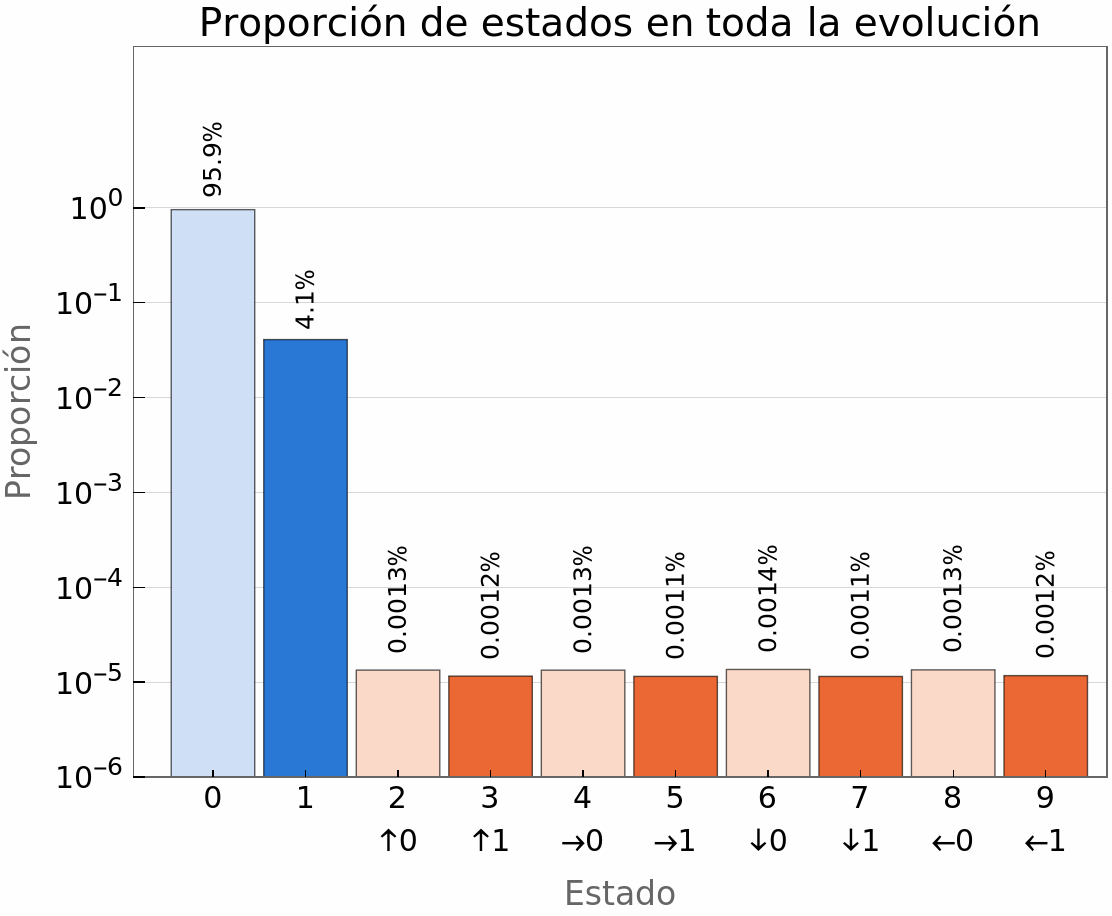
\includegraphics[width=0.9\linewidth]{img/experimentacion/duplicacion/langton/langton_RL_100x100_proporcion.png}
		\caption{11000 pasos con una configuración inicial vacía. }
		\label{fig:langton_RL_100x100_proporcion}
	\end{subfigure}
	\hfill 
	\begin{subfigure}[b]{0.45\textwidth}
		\centering
		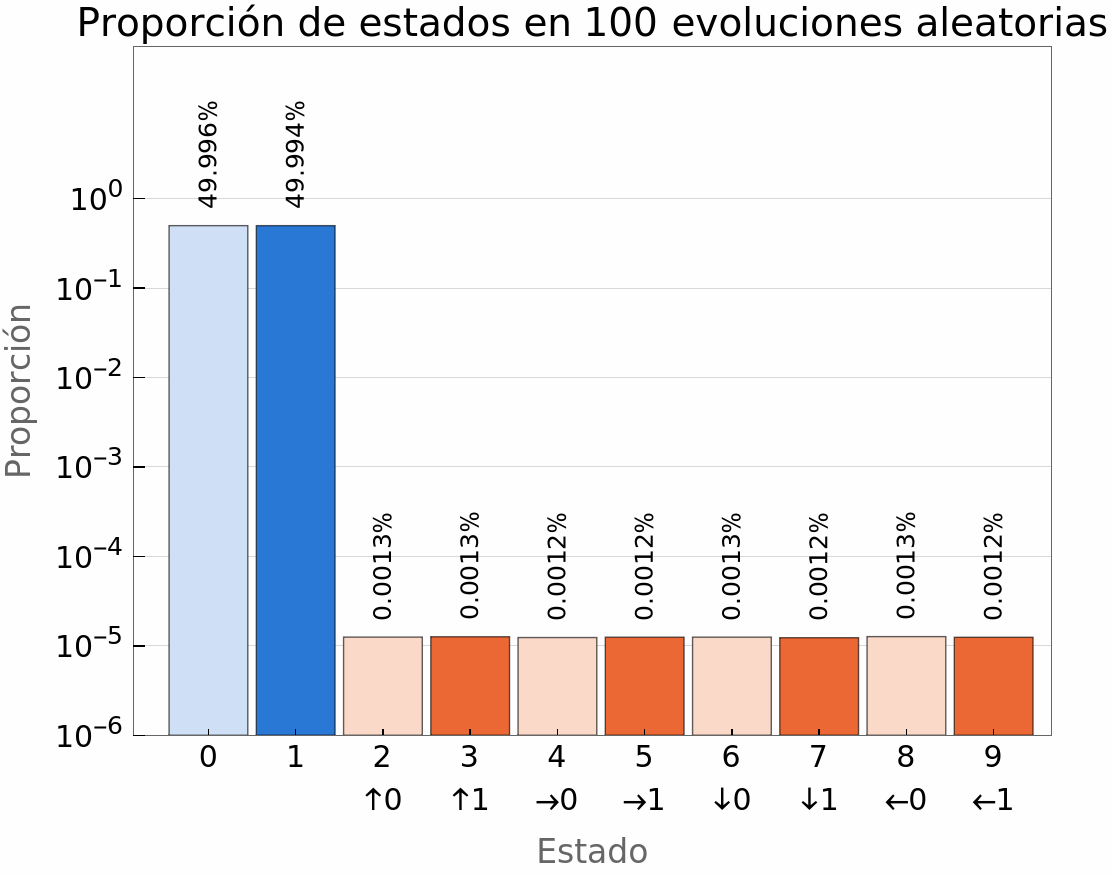
\includegraphics[width=0.9\linewidth]{img/experimentacion/duplicacion/langton/langton_RL_aleatorias_proporcion.png}
		\caption{100 pruebas durante 1,000 pasos con configuraciones iniciales aleatorias.}
		\label{fig:langton_RL_aleatorias_proporcion}
	\end{subfigure}
	\caption{Distribuciones de probabilidad de los 10 estados de una hormiga de Langton RL. Escala logarítmica.}
	\label{fig:langton_distribucion}
\end{figure}

\subsubsection{Capacidad de replicación}

Con una red neuronal dada por 2:8:ReLU \& 10:Linear, una tasa de aprendizaje de 0.001 y una pérdida objetivo de 0.0001, el autómata celular neuronal pudo replicar el comportamiento de una hormiga en el espacio a la perfección en tan solo 36 épocas usando \textit{one-hot encoding}. En la figura \ref{fig:langton_RL_paso_11000} se muestra el paso 11,000 de la hormiga generado en Mathematica y por el autómata celular neuronal en el simulador, y su coincidencia en el mismo punto.

\begin{figure}[htbp]
	\centering
	\begin{subfigure}[b]{0.45\textwidth}
		\centering
		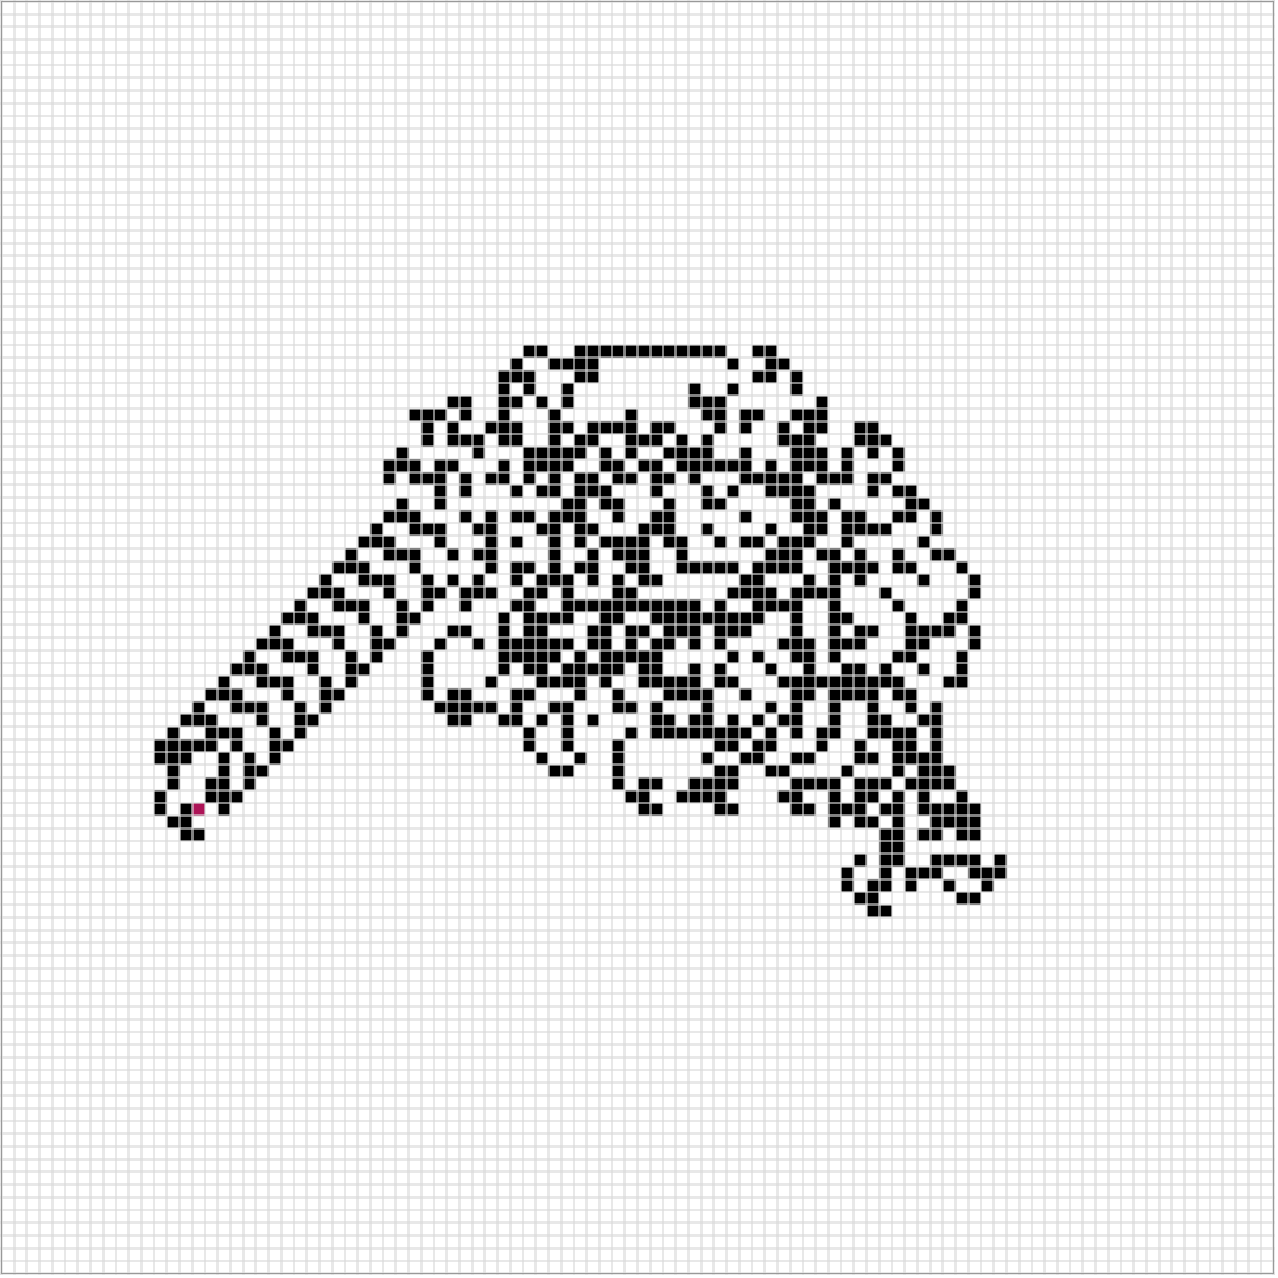
\includegraphics[width=0.7\linewidth]{img/experimentacion/duplicacion/langton/langton_RL_100x100_paso_11000.png}
		\caption{Evolución de la hormiga de Langton generada en Mathematica.}
		\label{fig:langton_RL_100x100_paso_11000}
	\end{subfigure}
	\hfill 
	\begin{subfigure}[b]{0.45\textwidth}
		\centering
		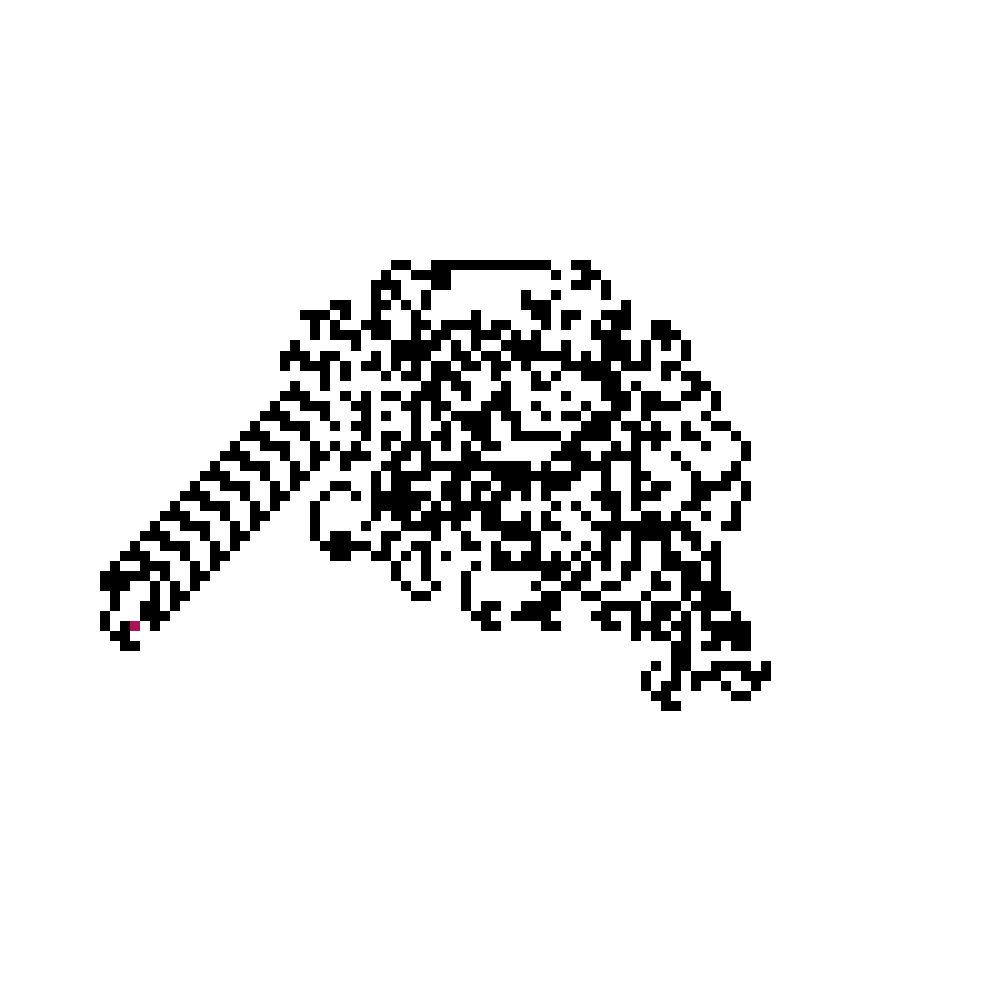
\includegraphics[width=0.67\linewidth]{img/experimentacion/duplicacion/langton/langton_RL_nca_100x100_paso_11000.png}
		\caption{Evolución del autómata celular neuronal originado en el simulador.}
		\label{fig:langton_RL_nca_100x100_paso_11000}
	\end{subfigure}
	\caption{Comparativa del agente Langton y el autómata celular neuronal entrenado después de 11,000 pasos con la misma configuración inicial. }
	\label{fig:langton_RL_paso_11000}
\end{figure}

\subsubsection{Colisión de múltiples hormigas}

Al colocar dos hormigas con la misma regla en el mismo espacio, su comportamiento suele ser independiente y ocurre sin errores hasta que se aproximan entre ellas. En la figura \ref{fig:langton_RL_nca_patrones_multi} se muestran los posibles patrones de dos hormigas donde una apunta a otra, en todos ellos, se realiza la sustitución correcta. El autómata celular neuronal extrapoló su conocimiento con una única hormiga para satisfacer estas condiciones. 

\begin{figure}[H]
	\centering
	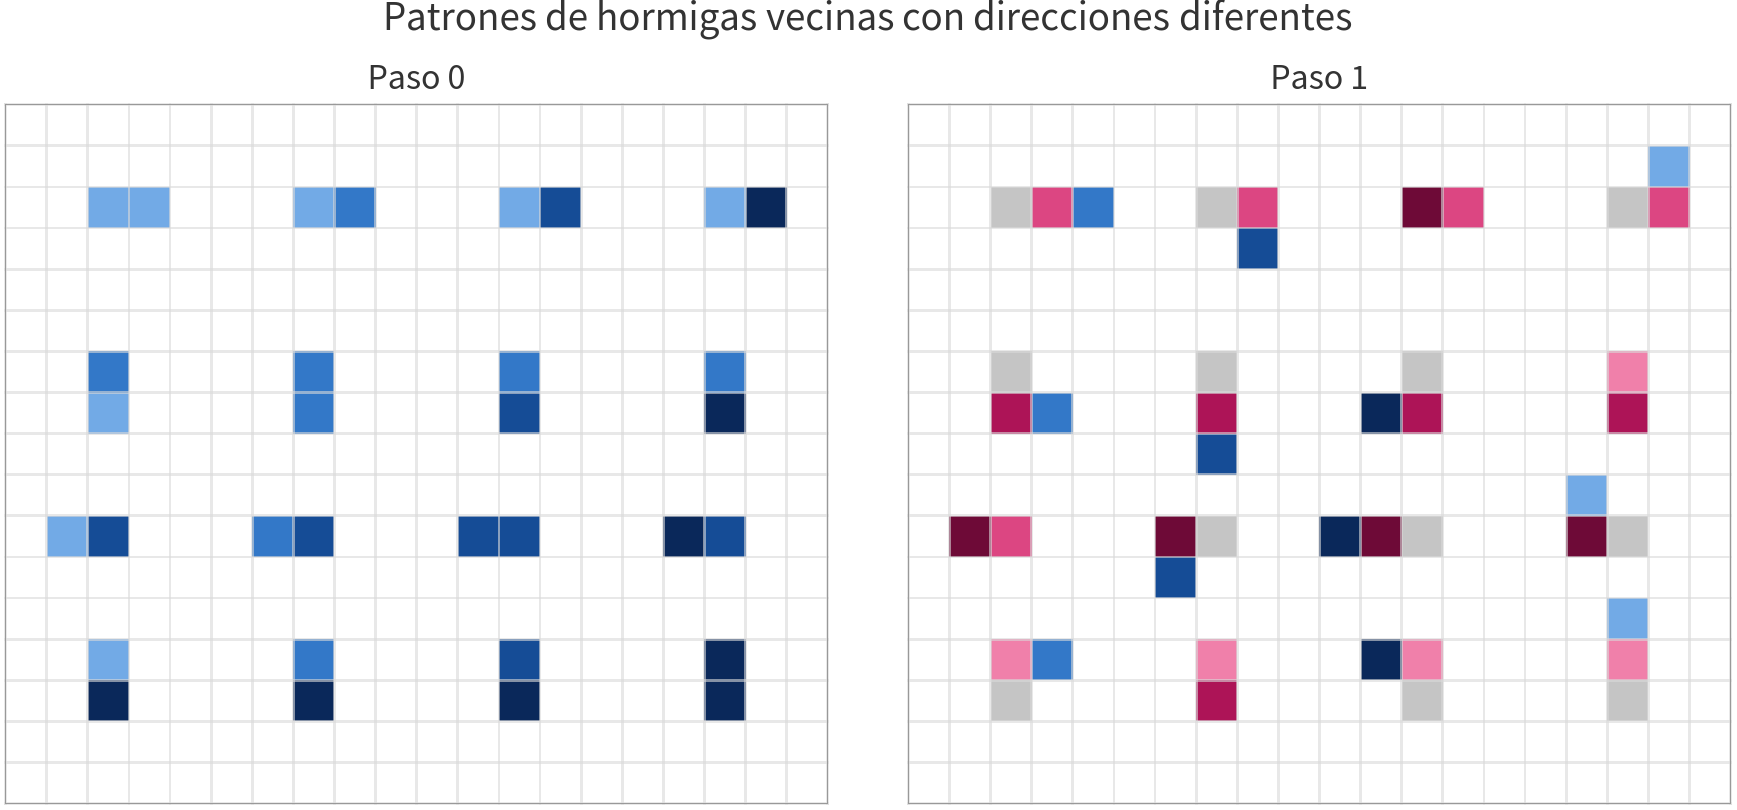
\includegraphics[width=0.5\linewidth]{img/experimentacion/duplicacion/langton/langton_RL_nca_patrones_multi.png}
	\caption{Preservación de hormigas vecinas bajo múltiples combinaciones.}
	\label{fig:langton_RL_nca_patrones_multi}
\end{figure}

Adicionalmente, en la figura \ref{fig:langton_RL_nca_patrones_combi} se muestran todos los patrones en donde dos hormigas colisionan en el siguiente paso. La solución que da el autómata celular neuronal es eliminar una de ellas.

\begin{figure}[H]
	\centering
	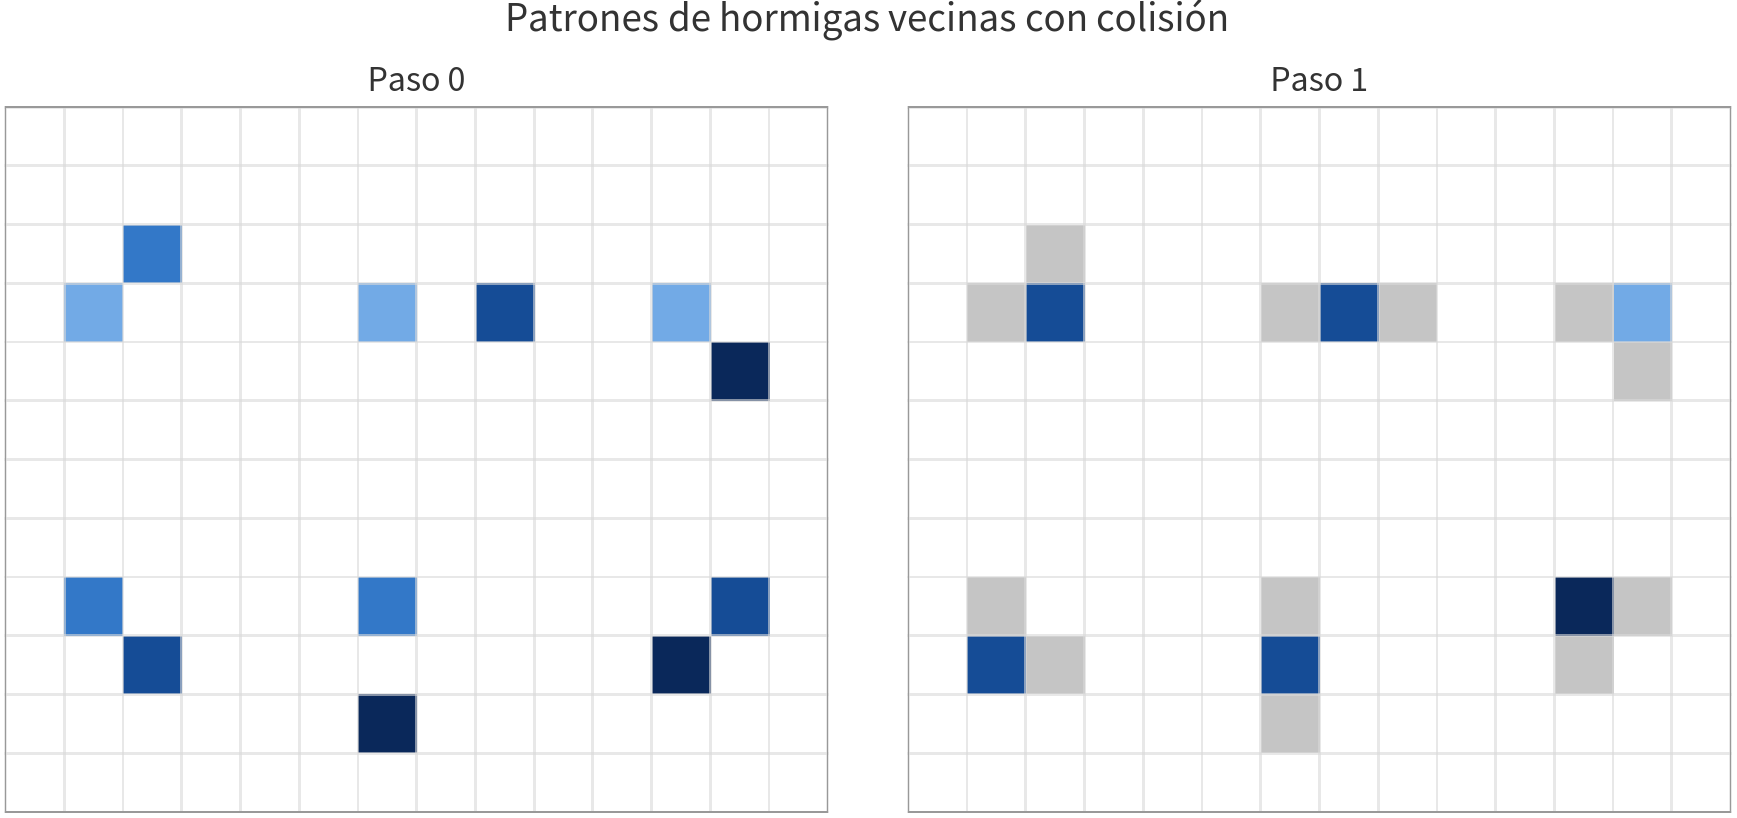
\includegraphics[width=0.5\linewidth]{img/experimentacion/duplicacion/langton/langton_RL_nca_patrones_combi.png}
	\caption{Eliminación de hormigas bajo múltiples combinaciones que colisionan en el paso 1.}
	\label{fig:langton_RL_nca_patrones_combi}
\end{figure}

Las simulaciones con múltiples hormigas deben tener una regla adicional que defina el comportamiento cuando hay colisiones, algunas opciones son:
\begin{itemize}
	\item Las hormigas son independientes: Cada hormiga ignora a las otras hormigas y solo le interesa el estado de la célula. Esta solución requiere incrementar el número de estados de manera proporcional al número de hormigas. Por lo que se requeriría definir el comportamiento de cuando hasta 4 hormigas colisionan en el mismo punto, situaciones menos probables que dependerían de preparar escenarios manuales para fomentar su aparición.
	\item Rotar sin avanzar: Es decir, si dos hormigas van a colisionar, se define una regla que ninguna ocupará ese espacio y en su lugar, cada una de ellas rota sobre su eje. Esta solución resuelve el problema, pero agrega un comportamiento adicional a la hormiga. 
	\item Actualización asíncrona: Las hormigas tienen un orden de prioridad, si se define se incrementa el número de estados, si no, rompe la definición de autómata celular.
	\item Combinación de hormigas: Solo una de ellas sobrevive cuando colisionan, resultado que fue inferido por el autómata celular neuronal.
\end{itemize}

Esta discrepancia se origina porque no existe una definición formal de cuál debe ser el comportamiento de múltiples hormigas en el mismo espacio, pues la idea fue concebida para una única hormiga.

\subsubsection{Crecimiento de estados}

Para finalizar, se explora el crecimiento del número de estados. La hormiga de Langton se generaliza a $n$ colores mediante una cadena de instrucciones, donde la letra $i$ indica el giro sobre una célula de color $i$ (R a la derecha, L a la izquierda), y la célula pasa al color $(i+1) \bmod n$. Con $n$ colores y cuatro direcciones, el autómata celular requiere $n + 4n = 5n$ estados, por lo que de 2 a 10 colores se pasa de 10 a 50 estados.

Para cada número de colores se generó un conjunto de datos con dos hormigas en un espacio de $30 \times 30$ con frontera periódica durante 10,000 pasos, usando la regla de rotar sin avanzar cuando dos hormigas van a colisionar. Para cada $n$ se eligió la regla que distribuye los colores de forma más uniforme, ignorando aquellas que repiten una más corta (por ejemplo, RRLRRL se comporta como RRL). La vecindad es un rombo de radio 2 (13 células), pues una célula necesita saber si otra hormiga a dos células de distancia también apunta hacia ella. Todas las redes tienen la forma 4:64:ReLU \& $5n$:Linear con \textit{one-hot encoding}, una tasa de aprendizaje inicial de 0.001 que se reduce a la mitad cuando la pérdida no mejora en 20 épocas, una pérdida objetivo de $1 \times 10^{-7}$ y semilla 42.

En la tabla \ref{tab:langton_colores} se observa que el número de estados casi no afecta el entrenamiento: todas las configuraciones alcanzaron la pérdida objetivo en menos de 90 épocas y menos de 100 segundos. Además, el número de épocas no crece de forma monótona con el número de colores. A partir de 8 colores la tasa de aprendizaje se redujo una vez, a 0.0005. Ocho de las nueve redes reproducen los 10,000 pasos de su evolución sin errores. La excepción es la regla RRRLLL (6 colores), que tiene un único error en 9 millones de células, en un paso donde las hormigas colisionan, lo que hace que la evolución diverja en el paso 7,028.

\begin{table}[H]
	\centering
	\begin{tabular}{c c l c c c}
		\toprule
		Colores & Estados & Regla & Épocas & Pérdida final & Tiempo \\
		\midrule
		2  & 10 & RL         & 22 & $5.18 \times 10^{-8}$ & 25.6 s \\
		3  & 15 & RLL        & 63 & $3.83 \times 10^{-8}$ & 73.8 s \\
		4  & 20 & RLLR       & 16 & $3.27 \times 10^{-8}$ & 20.0 s \\
		5  & 25 & RLRLL      & 44 & $7.81 \times 10^{-8}$ & 51.3 s \\
		6  & 30 & RRRLLL     & 68 & $4.35 \times 10^{-8}$ & 75.4 s \\
		7  & 35 & RLRLRLL    & 77 & $6.77 \times 10^{-9}$ & 85.7 s \\
		8  & 40 & RLRLRLRR   & 63 & $1.57 \times 10^{-8}$ & 70.4 s \\
		9  & 45 & RLRLRLLRL  & 63 & $2.31 \times 10^{-8}$ & 73.7 s \\
		10 & 50 & RLRLRLRRRL & 87 & $2.38 \times 10^{-9}$ & 97.3 s \\
		\bottomrule
	\end{tabular}
	\caption{Entrenamiento de la hormiga de Langton con dos hormigas de 2 a 10 colores. Espacio de $30 \times 30$, 10,000 pasos, red 4:64:ReLU \& $5n$:Linear con \textit{one-hot encoding}, pérdida objetivo $1 \times 10^{-7}$.}
	\label{tab:langton_colores}
\end{table}

Sin embargo, reproducir la evolución de entrenamiento no implica haber aprendido la regla. Con la regla de 10 colores, una única hormiga orientada hacia la izquierda, en el centro de un espacio de $100 \times 100$ con frontera periódica, evoluciona sin errores hasta el paso 12,455, donde la hormiga se divide en dos. La hormiga gira y avanza correctamente, pero la célula que deja no cambia de color y conserva una hormiga girada, como si hubiera estado bloqueada por otra. Es decir, el autómata celular neuronal aplica la regla de colisión aprendida de los datos con dos hormigas en un patrón que nunca vio durante el entrenamiento, aunque no haya otra hormiga cerca.

Con este último experimento observamos que el autómata celular neuronal puede reproducir comportamientos complejos con un número creciente de estados. El sistema tradicional pudo ser replicado con exactitud y, con hasta 10 colores (50 estados, $50^{13}$ patrones y $50^{50^{13}}$ reglas totales), las redes reprodujeron su evolución de entrenamiento, es decir, extrajeron la parte de la función de transición presente en esos datos. Sin embargo, fuera de ellos aparecen errores como la división de la hormiga, por lo que reproducir la evolución no garantiza haber extraído la función de transición en su totalidad.

Además, se pudo generalizar el comportamiento de una hacia dos hormigas cuando no colisionan pero sí son vecinas, comportamiento que no estuvo presente durante el entrenamiento. Finalmente, aplicó la eliminación de hormigas que, aunque pudo haber utilizado cualquier función para definir ese comportamiento, fue constante en todas las combinaciones donde colisionaban.

Esta serie de tres experimentos (juego de la vida, modelo de \textit{sandpile} y hormiga de Langton) ayudaron no solo a probar las capacidades de replicación de la red neuronal al momento de experimentar con sistemas complejos, sino que adicionalmente ayudaron a 
\begin{itemize}
	\item Definir la mejor estructura de la red neuronal: Se encontró que ReLU en las capas ocultas y Linear en la capa de salida suele tener los mejores resultados. Además, no es necesario tener redes muy profundas, en su lugar, es recomendado tener pocas capas con mayor número de neuronas cada una. 

	\item Seleccionar hiperparámetros: Comparando métodos de reducción de tasa de aprendizaje, se concluyó que una reducción dinámica es una opción viable cuando la pérdida empieza a tener un comportamiento oscilatorio. 

	\item Definir la capa de entrada: Esto mediante una codificación \textit{one-hot} que elimina la linealidad entre los datos y agiliza el entrenamiento de la red neuronal drásticamente. 
	
	\item Comprender la generalización de comportamientos: Cómo se adapta ante escenarios nunca antes vistos o muy poco frecuentes pero manteniendo su dinámica principal.
\end{itemize}

Estas tareas ayudaron a implementar mejoras dentro del simulador así como configurar el autómata celular neuronal para los próximos experimentos, en donde se busca imitar el comportamiento de sistemas complejos que se encuentren en la naturaleza.


	\chapter{Replicación de sistemas complejos naturales}
\label{chap:naturales}

El autómata celular neuronal tiene la capacidad de replicar sistemas bidimensionales con una regla muy bien definida. La regla obtenida no pudo replicar todos los escenarios en todos los experimentos; sin embargo, sí conserva una fuerte adherencia al comportamiento original. 

Hasta el momento, solo se experimentó con simulaciones en donde tenemos un control absoluto de todos los escenarios, pues al tener una regla bien definida y, más aún, un sistema del cual obtener los datos de entrenamiento, tenemos la referencia exacta de cómo la evolución debiera ser. Pero en la vida real no es posible obtener todas estas evoluciones, y los siguientes experimentos buscan dar paso al objetivo central de esta investigación: brindar a los autómatas celulares la capacidad de aprender reglas del entorno con la referencia evolutiva y no con la regla del sistema. 

Dicho esto, en esta parte se siguen tres experimentos principales que buscan dar propósito a este sistema: la simulación de la propagación de un incendio, la simulación de tormentas y el crecimiento de un moho mucilaginoso.


	\section{Simulación de la propagación}

El presente experimento busca analizar la propagación del fuego. Una opción para simularlo pudiera ser mediante la definición manual de la regla que gobierne el sistema. Por ejemplo, podemos definir tres estados: vivo, quemado y quemándose, en donde toda célula viva que tenga un vecino quemándose se quema en el siguiente paso, y toda célula quemándose se apaga. Si bien esta definición podría mostrar dinámicas de propagación, no está definida mediante un sistema real, objetivo de esta investigación.

Este experimento se alimenta del conjunto de datos FLAME~3 \cite{hopkins2024flame3datasetunleashing}, que captura la quema de Hanna Hammock en 2023. Sus autores utilizaron un dron que captura imágenes térmicas con vista cenital\footnote{Cenit: punto más alto en el cielo, ubicado a 90° por encima del observador \cite{plano_cenital}.} para la gestión de incendios forestales. Este conjunto de datos contiene tres carpetas de imágenes: en formato ``tiff'', que registran la temperatura, en ``jpg'' con vista térmica y en ``jpg'' regular.

\subsection{Preprocesamiento de los datos}

Para la limpieza del conjunto de datos, se procedió de la siguiente manera: 

\begin{enumerate}
	\item Selección de conjuntos de mayor representación: El conjunto de datos completo contiene la vista de tres diferentes zonas, de las cuales solo los \textit{plot} 1 y 2 contienen la secuencia en formato ``tiff'' durante la quema. De estos conjuntos, se consideran las siguientes dos particiones como representantes de la propagación:

	\begin{itemize}
		\item flame\_plot\_1 (\textit{plot} 1 de Kaggle): de la imagen 662 a la 777, 116 \textit{frames}
		\item flame\_plot\_2 (\textit{plot} 2 de Kaggle): de la imagen 1189 a la 1254, 66 \textit{frames}
	\end{itemize}
	
	Estos rangos se caracterizan por mostrar la propagación del fuego de un $\sim 2\%$ a un $\sim 86\%$ del espacio en flame\_plot\_1 y de un $\sim 4\%$ a casi el $100\%$ en flame\_plot\_2. Iniciar con fuego dentro del sistema es esencial para que la red neuronal no infiera combustión espontánea. Además, se seleccionan estos rangos por ser los que incluyen una propagación con velocidad constante. 

	\item Ajuste de posición: El dron se mueve por el viento, por lo que un desajuste de varios píxeles obliga a incrementar la vecindad en cada dirección para capturar el error. Para esto, se opta por la siguiente técnica que ajusta la imagen:

	\begin{enumerate}
		\item Se mide el desplazamiento entre pares de imágenes mediante correlación de fase con precisión de $1/20$ de píxel. Para que el movimiento del fuego no se confunda con el movimiento de la cámara, solo se compara la textura del suelo frío (menos de 50 °C en ambas imágenes y a más de 12 píxeles del fuego).
		\item Cada imagen se compara no solo con la siguiente, sino con las que están a 1, 2, 4, 8, \dots, 128 imágenes de distancia. Al encadenar únicamente imágenes consecutivas, el error de cada medición se acumula a lo largo de la secuencia.
		\item Con todas las mediciones se resuelve la posición de cada imagen respecto a la primera mediante mínimos cuadrados robustos (pérdida de Huber), lo que reduce el peso de las mediciones erróneas.
		\item Cada imagen se desplaza a la posición de la primera mediante interpolación bilineal. La corrección máxima fue de 6.57 píxeles en flame\_plot\_1 y de 7.69 píxeles en flame\_plot\_2.
	\end{enumerate}

	Sin embargo, las imágenes resultantes generan bordes negros que representan el movimiento de la imagen. Esto genera ruido en los bordes, lo que nos obliga a reducir el tamaño de los datos.
	
	\item Eliminación de ruido residual: Al desplazar cada imagen, la zona que queda fuera de la imagen original se rellena con píxeles negros (sin dato). Para ello, se extrae de la imagen el cuadrado de mayor tamaño que no tenga ruido en ninguna imagen de la secuencia (esto para ambas secuencias), y se obtiene la imagen reducida, tal como se muestra en la figura \ref{fig:experimentacion:natuales:Flame3:clean_03}.
	
	\item Escalado de la evolución: Con la imagen reducida, se aplican operaciones de convolución con el objetivo de reducir el tamaño de la imagen a $100 \times 100$ píxeles y disminuir la complejidad de la dinámica. Sin embargo, este método reduce el conjunto de entrenamiento, porque disminuye la cantidad de vecindades que podemos extraer. 
	
	 \item Discretización: El objetivo de este experimento es simular la propagación del fuego y no la propagación de la temperatura. Estos datos están estrechamente relacionados, pero si únicamente consideramos los registros de temperatura, ignoramos que el fuego no se puede propagar dos veces por el mismo terreno. Es por esto que el sistema debe conocer cuándo hay un incendio y distinguir si los registros corresponden a su temperatura antes o después del fuego. 
	 
	 Para resolver esto, se discretizan los píxeles y se ajustan a 18 estados según las temperaturas de la tabla \ref{tab:flame_states_proportion}. Los estados $ \mathcal{S}_b = \{0, 1, \dots, 11\}$ corresponden a las temperaturas normales y su incremento conforme el fuego se propaga y la temperatura aumenta, mientras que los estados $\mathcal{S}_t = \{12, 13, \dots, 17\}$ corresponden al enfriamiento del sistema. Sea $\tau_{\vec{i}}(t) \in \{0, 1, \dots, 11\}$ el estado de temperatura de la célula $\vec{i}$, $T_{\vec{i}}(t)$ su temperatura en °C y $m_{\vec{i}}$ la temperatura mínima que ha registrado desde que se quemó. Definimos la siguiente regla para asignar los estados:
	 \[
	 	\sigma_{\vec{i}}(t + 1) \in
	 	\begin{cases}
	 		\mathcal{S}_t & \text{si } \tau_{\vec{i}}(t + 1) < \tau_{\vec{i}}(t) \\
	 		\mathcal{S}_b & \text{si } \sigma_{\vec{i}}(t) \in \mathcal{S}_t,\ T_{\vec{i}}(t + 1) > m_{\vec{i}} + 30\,^\circ\mathrm{C} \\
	 		\text{el de } \sigma_{\vec{i}}(t) & \text{en otro caso}
	 	\end{cases}
	 \]
	 donde una célula en $\mathcal{S}_b$ toma el estado $\tau_{\vec{i}}(t + 1)$ y una en $\mathcal{S}_t$ toma el estado $12 + \lfloor \tau_{\vec{i}}(t + 1) / 2 \rfloor$, por lo que los estados quemados agrupan las temperaturas de dos en dos.

	 Es decir, si se enfría pasa a un estado quemado, pero si su temperatura aumenta nuevamente más de 30 °C sobre el mínimo registrado desde que se quemó, deja de estar quemada y regresa a su estado de temperatura.
	 
\end{enumerate}

\begin{table}[htbp]
	\centering
	\footnotesize
	\begin{tabular}{ccccc}
		\toprule
		& & & \textbf{Porcentaje en} & \textbf{Porcentaje en} \\
		\textbf{Estado} & \textbf{Tipo} & \textbf{Temperatura} & \textbf{flame\_plot\_1} & \textbf{flame\_plot\_2} \\ \midrule
		0 & \multirow{12}{*}{Temperatura} & 25.3--59.0 & 49.13 & 16.74 \\
		1 &  & 59.0--72.9 & 1.45 & 4.07 \\
		2 &  & 72.9--90.1 & 0.87 & 2.25 \\
		3 &  & 90.1--111.4 & 0.77 & 1.35 \\
		4 &  & 111.4--137.6 & 0.76 & 1.15 \\
		5 &  & 137.6--170.0 & 0.70 & 1.11 \\
		6 &  & 170.0--210.0 & 0.71 & 1.10 \\
		7 &  & 210.0--259.5 & 0.74 & 1.25 \\
		8 &  & 259.5--320.6 & 0.83 & 1.43 \\
		9 &  & 320.6--396.1 & 0.82 & 1.92 \\
		10 &  & 396.1--489.3 & 0.15 & 2.13 \\
		11 &  & 489.3--604.6 & 0.00 & 0.28 \\ \midrule
		12 & \multirow{6}{*}{Quemado} & 25.3--72.9 & 23.82 & 10.79 \\
		13 &  & 72.9--111.4 & 9.24 & 15.88 \\
		14 &  & 111.4--170.0 & 5.72 & 16.59 \\
		15 &  & 170.0--259.5 & 3.25 & 13.34 \\
		16 &  & 259.5--396.1 & 1.03 & 7.81 \\
		17 &  & 396.1--604.6 & 0.01 & 0.80 \\ \bottomrule
	\end{tabular}
	\caption{Estados de FLAME~3 con 12 estados de temperatura y 6 de quemado, su rango de temperatura en °C y el porcentaje de células en cada estado.}
	\label{tab:flame_states_proportion}
\end{table}

	El resultado se muestra en la figura \ref{fig:flame_clean_process}, que presenta la conversión de una imagen durante cada uno de los pasos ya mencionados. Cabe mencionar que este proceso no se realiza sobre las imágenes ``jpg'', sino sobre las ``tiff'', ya que las primeras ajustan los colores según los rangos de temperatura presentes, por lo que dos temperaturas pueden tener el mismo color asociado en diferentes imágenes, mientras que las ``tiff'' almacenan la temperatura de cada posición.
	
	\begin{figure}[htbp]
		\centering
		\begin{subfigure}[b]{0.35\textwidth}
			\centering
			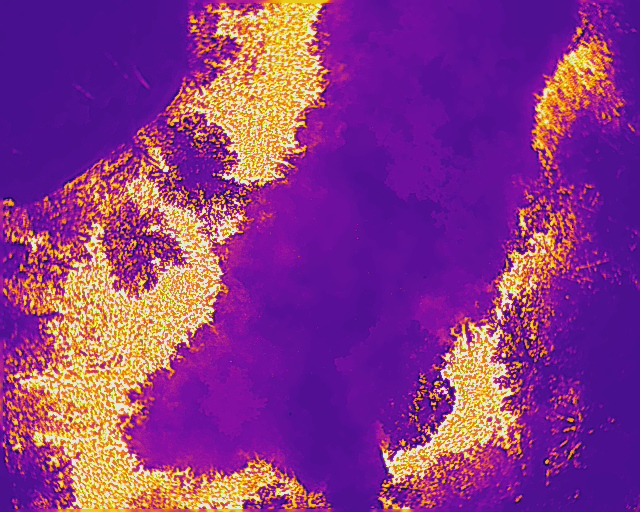
\includegraphics[width=\linewidth]{img/experimentacion/naturales/Flame3/clean_01.jpg}
			\caption{Imagen original}
			\label{fig:experimentacion:natuales:Flame3:clean_01}
		\end{subfigure}
		\hfill 
		\begin{subfigure}[b]{0.35\textwidth}
			\centering
			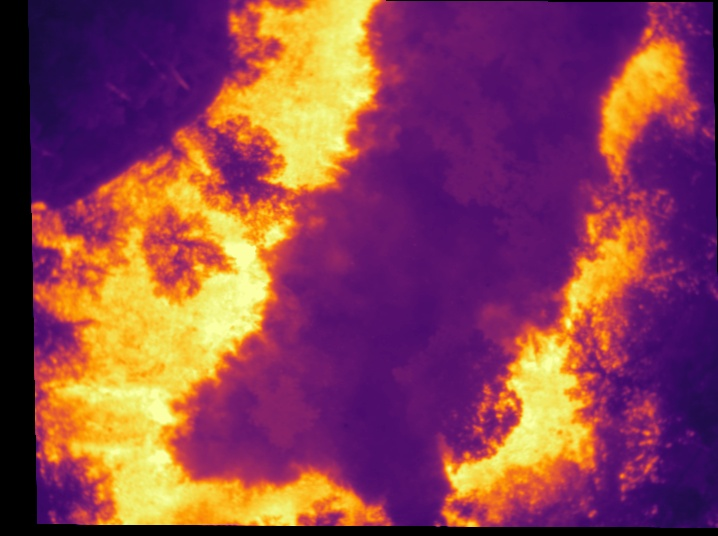
\includegraphics[width=\linewidth]{img/experimentacion/naturales/Flame3/clean_02.jpg}
			\caption{Ajuste de posición}
			\label{fig:experimentacion:natuales:Flame3:clean_02}
		\end{subfigure}
		\hfill 
		\begin{subfigure}[b]{0.30\textwidth}
			\centering
			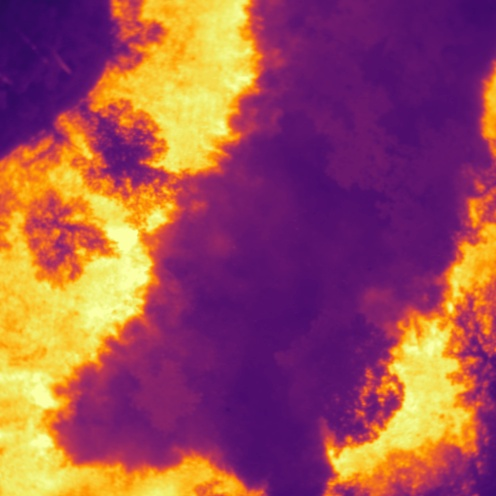
\includegraphics[width=0.75\linewidth]{img/experimentacion/naturales/Flame3/clean_03.jpg}
			\caption{Eliminación de ruido residual}
			\label{fig:experimentacion:natuales:Flame3:clean_03}
		\end{subfigure}
		\hfill 
		\begin{subfigure}[b]{0.30\textwidth}
			\centering
			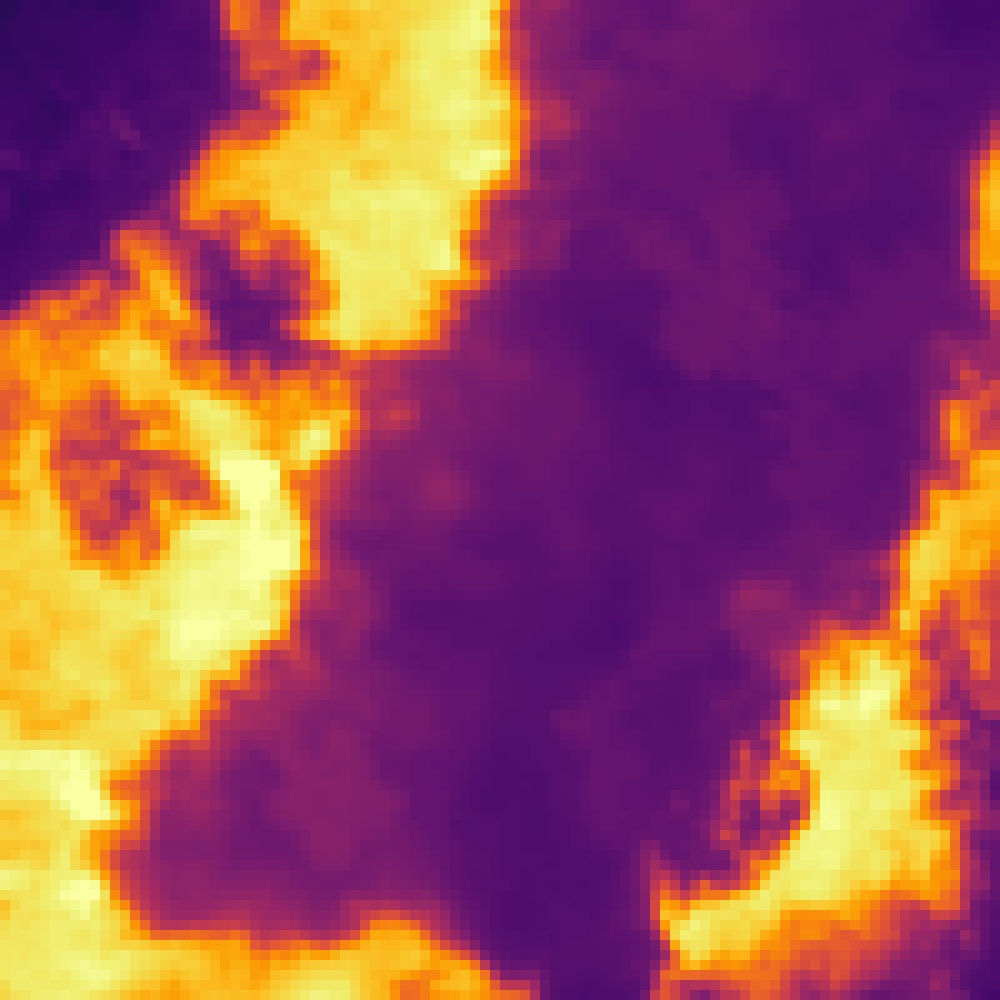
\includegraphics[width=0.75\linewidth]{img/experimentacion/naturales/Flame3/clean_04.jpg}
			\caption{Reducción por convolución}
			\label{fig:experimentacion:natuales:Flame3:clean_04}
		\end{subfigure}
		\hfill 
		\begin{subfigure}[b]{0.30\textwidth}
			\centering
			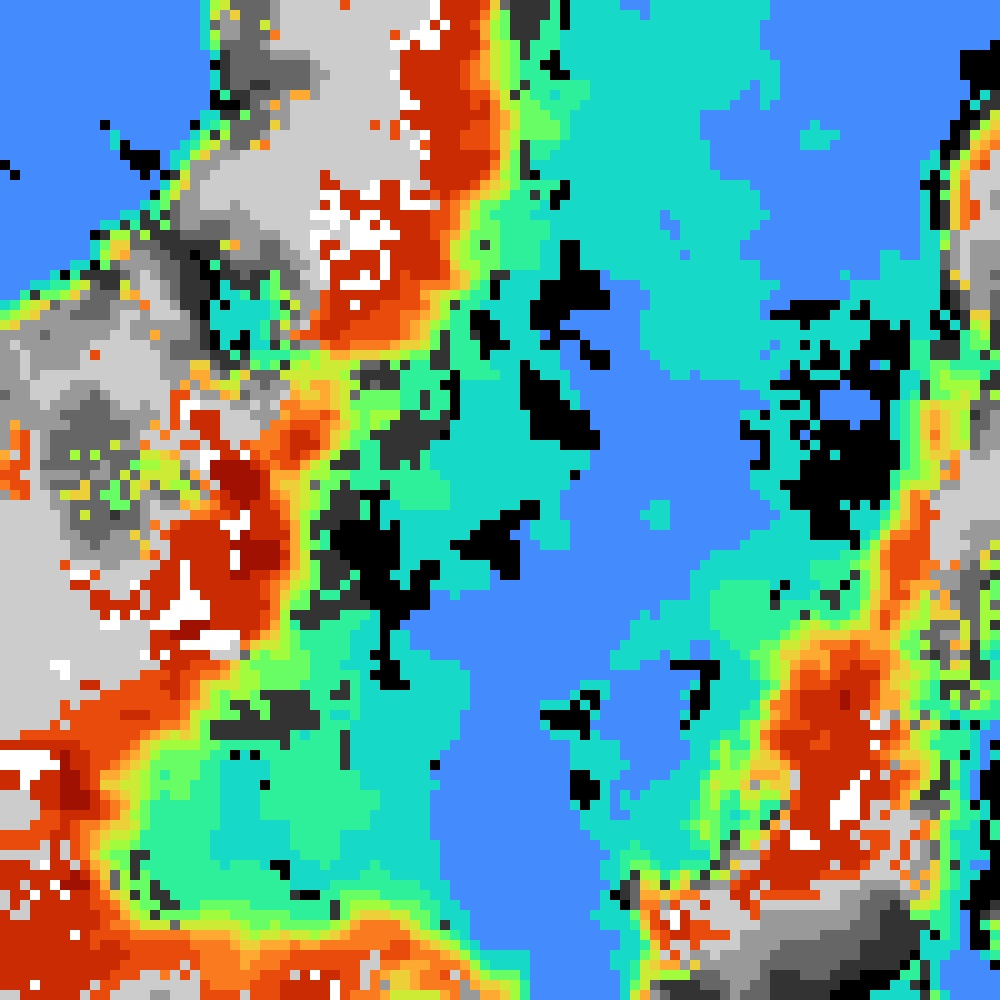
\includegraphics[width=0.75\linewidth]{img/experimentacion/naturales/Flame3/clean_05_18estados.jpg}
			\caption{Segmentación en 18 estados}
			\label{fig:experimentacion:natuales:Flame3:clean_05}
		\end{subfigure}
		\caption{Proceso de limpieza sobre la imagen 1204 del \textit{plot} 2 de Kaggle.}
		\label{fig:flame_clean_process}
	\end{figure}
	
		Con estos datos, obtenemos un total de $116 + 66 = 182$ imágenes de $100 \times 100$ píxeles, o mejor dicho, células. Estas tienen una distribución de estados como se muestra en la figura \ref{fig:flame_distribucion_estados}, en donde la mayoría de las células se ajustan a los valores más fríos, es decir, terreno que aún no se quema o que ya se enfrió después del fuego, y las zonas más calientes tienen menor representación. Sin embargo, se considera un rango aceptable dadas las capacidades de extracción de comportamientos que se apreciaron durante los experimentos de la hormiga de Langton.
	
	\begin{figure}[htbp]
		\centering
		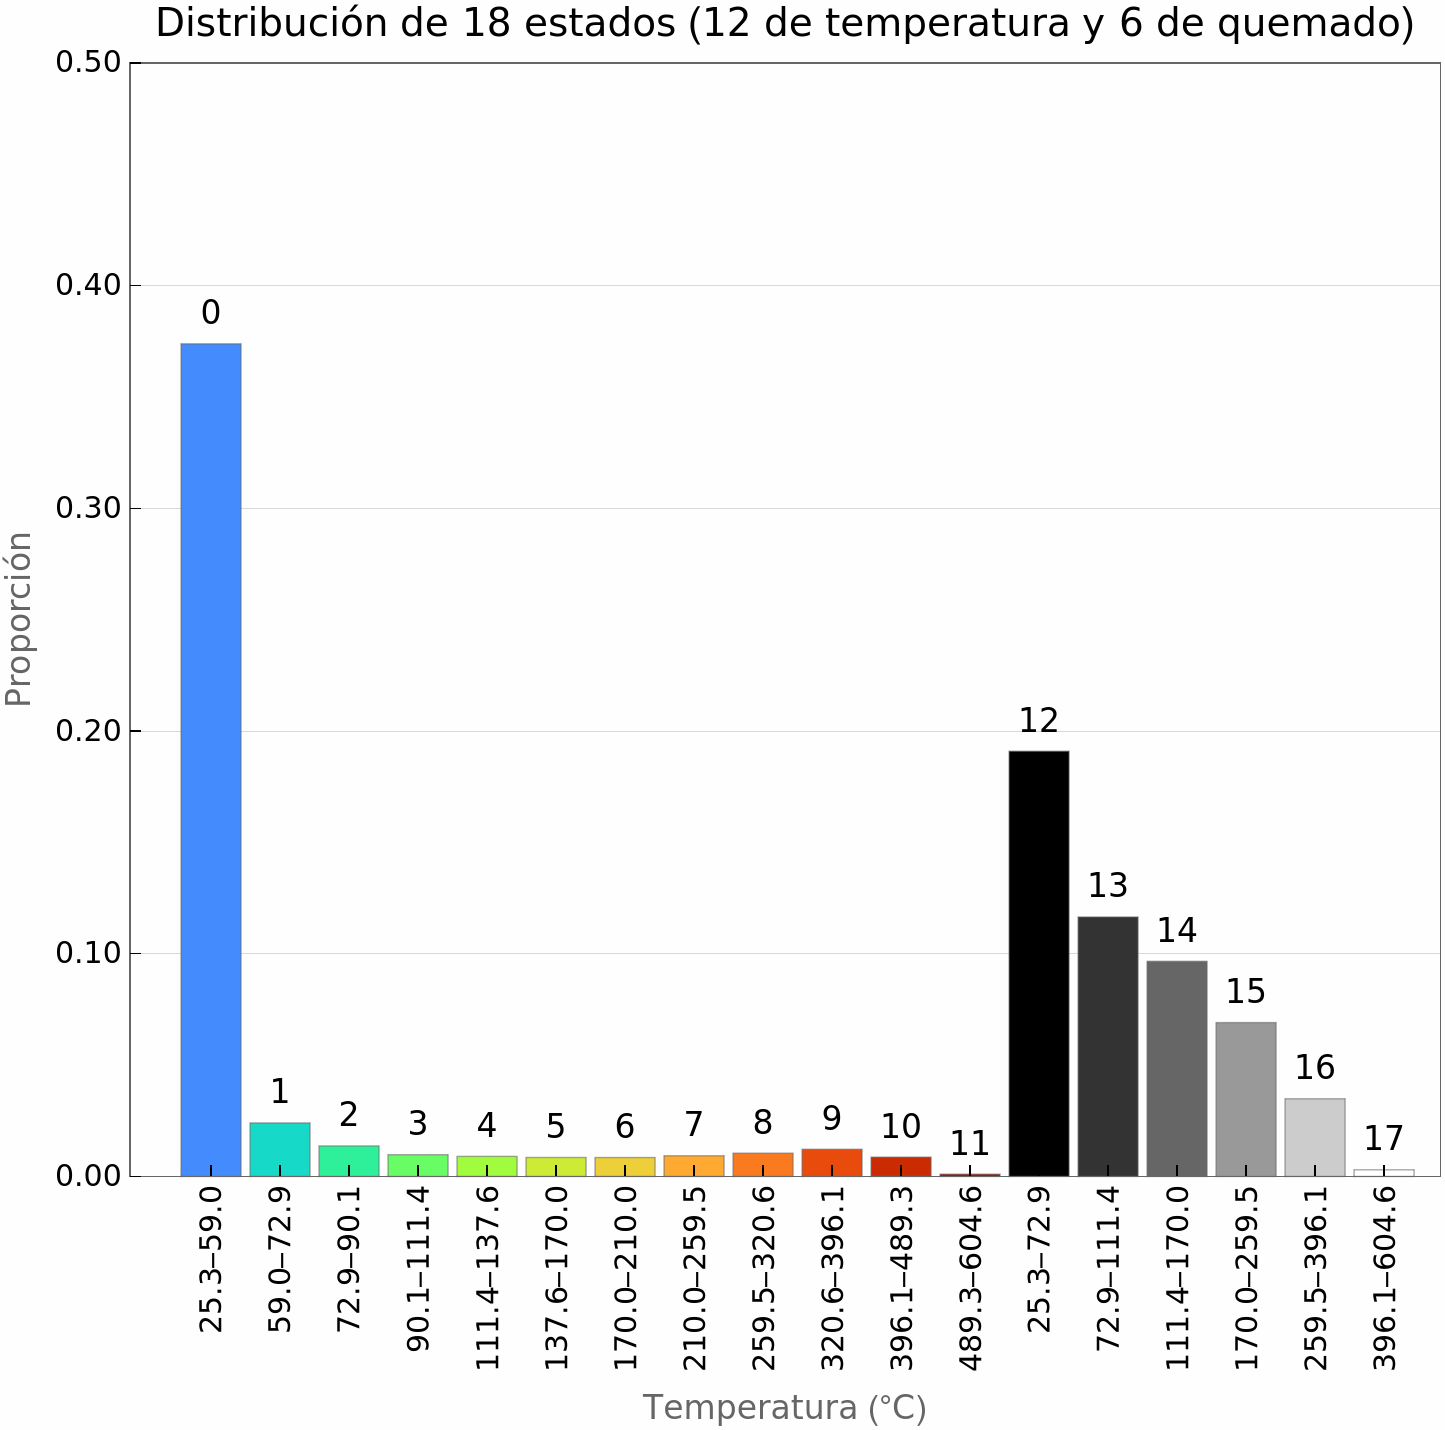
\includegraphics[width=0.6\linewidth]{img/experimentacion/naturales/Flame3/distribucion_estados18.png}
		\caption{Distribución de los 18 estados del conjunto de imágenes de entrenamiento de FLAME~3 para la predicción de propagación del fuego.}
		\label{fig:flame_distribucion_estados}
	\end{figure}
	
	Cabe mencionar que este método de limpieza de datos fue el que tuvo un mejor rendimiento y fue diseñado con base en los resultados de experimentos previos. 

	Adicionalmente, se hace la distinción entre el error de cuantización y el error de la dinámica: el primero mide qué tanta información se pierde al convertir una temperatura en un estado; no está relacionado con la red neuronal, únicamente mide la pérdida de información al discretizar. El segundo se refiere al error que tiene la red neuronal en su predicción, es decir, compara los datos discretizados con lo que predice la red.

	Por ejemplo, al discretizar en 15 estados con una escala logarítmica, tenemos un error de cuantización de 5.2 °C, es decir, en promedio cada célula difiere de su temperatura original por esa cantidad. A continuación, en la tabla \ref{tab:flame_experiments} se muestran múltiples configuraciones que ayudaron a obtener esta configuración final. El porcentaje de error en la predicción compara la red neuronal entrenada contra no hacer nada, es decir, contra suponer que cada célula conserva el mismo estado. Por esto, si es menor al 100\%, significa que la red mejora en relación con no hacer nada; en el caso contrario, es peor que no hacer nada.
	

	\begin{table}[htbp]
		\centering
		\footnotesize
		\setlength{\tabcolsep}{4pt}
		\setlength{\belowrulesep}{2pt}
		\begin{tabularx}{\textwidth}{p{0.24\textwidth}Xp{0.21\textwidth}}
			\toprule
			\textbf{Modificación} & \textbf{Resultado} & \textbf{Aporte a la configuración final} \\ \midrule
			Segmentar los estados mediante \textit{k-means} &
			Codo en $k = 4$. El estado 0 abarca del 66 al 99\% de las células y todo lo que supera 238 °C queda en un solo estado. &
			Escala logarítmica de 15 estados que distingue las zonas más calientes. \\ \midrule
			
			Tomar una imagen de cada 1, 3 o 6 &
			Con 6, la red de vecindad $9 \times 9$ y configuración 2:32 supera a la predicción sin cambio (exactitud de 0.588 contra 0.552 en el \textit{plot} de prueba). &
			Se toma una imagen de cada 6. \\ \midrule
			
			Cambiar el número de estados (de 4 a 50, logarítmicos y \textit{k-means}) &
			Con 50 estados se reduce el error de cuantización a 1.6 °C, pero no el error de la dinámica. Con 4 estados aumenta a 19 °C. &
			Entre 12 y 15 estados de temperatura (error de $\sim 5.2$ °C). \\ \midrule
			
			Quitar las imágenes de la ignición &
			Casi ninguna red supera a la predicción sin cambio ni enciende células. Las redes entrenadas con la ignición y evaluadas sin ella tienen menor error en la simulación libre. &
			Las secuencias inician con el fuego ya presente y en propagación. \\ \midrule
			
			Quitar el conjunto casi sin fuego &
			En ese conjunto casi nada cambia: la predicción sin cambio tiene un error de 1.92 °C y no permite saber si la red aprende. &
			Se descartan las secuencias casi sin fuego. \\ \midrule
			
			Unir los estados más fríos (0--2 en 13 estados; 0--3 en 12 estados) &
			Con 13, el error en la simulación libre baja de 21.9 a 19.2 °C. Con 12 estados, la mejor red tiene el 92.8\% del error de la predicción sin cambio. &
			12 estados de temperatura (estado 0 = 25.3--59.0 °C). \\ \midrule
			
			Rotar las imágenes de entrenamiento 0, 90, 180 y 270° &
			El error de un paso baja del 94 al 91\% del de la predicción sin cambio; la simulación libre no mejora de forma consistente. &
			No se usa. \\ \midrule
			Reducir a $200 \times 200$ &
			Error del 90\% de la predicción sin cambio, pero enciende menos células: solo el 50\% y el 20\% de las que se encienden tienen fuego vecino. &
			Se mantiene $100 \times 100$. \\ \midrule
			
			Agregar el combustible como clase fija &
			La red casi no enciende células (menos del 1.4\%) y no mejora a la red sin clase. &
			No se usa. \\ \midrule
			
			Bandera de quemado: el estado se duplica si la célula alguna vez llegó a 135.9 °C o más &
			5 veces más células encendidas, con precisión de $\approx 0.2$. Error de un paso de $\approx 22$ °C contra 16 °C de la predicción sin cambio, y la simulación libre diverge (37--67 °C contra 18 °C). &
			Estado de quemado por enfriamiento de la célula y no por un umbral fijo. \\ \midrule
			
			Quemado al enfriarse, con 12 estados de quemado (24 estados) y sin umbral &
			28,537 regresos de quemado a no quemado, el 92\% por subidas de un solo estado (ruido); el estado 23 nunca aparece. &
			Estados de quemado agrupados de dos en dos y umbral de 30 °C (9,102 regresos). \\ \bottomrule
			
		\end{tabularx}
		\caption{Modificaciones al preprocesamiento de FLAME~3 previas a la configuración final. Predicción sin cambio: suponer que el siguiente paso es igual al actual. Salvo que se indique otra cosa, vecindad $9 \times 9$, 2 capas de 32 neuronas e imágenes de $100 \times 100$.}
		\label{tab:flame_experiments}
	\end{table}
	
	Antes de definir estados de quemado o de combustible, usar \textit{one-hot encoding} no mejoraba los resultados (tabla \ref{tab:flame_onehot}). Con \textit{one-hot} la red aprende mejor los datos de entrenamiento, pero tiene una peor generalización: su error es mayor en casi todos los experimentos y entre 2 y 5 veces más redes terminan la simulación libre con más del doble de error que la predicción sin cambio. La excepción es la bandera de quemado, en donde los estados ya no están ordenados por temperatura.

	\begin{table}[htbp]
		\centering
		\footnotesize
		\setlength{\tabcolsep}{4pt}
		\begin{tabular}{llcccc}
			\toprule
			& & \textbf{Error} & \textbf{Redes} & & \\
			& & \textbf{respecto a} & \textbf{mejores que} & & \\
			& & \textbf{la predicción} & \textbf{la predicción} & \textbf{Redes que} & \textbf{Pérdida al} \\
			\textbf{Experimento} & \textbf{One-hot} & \textbf{sin cambio} & \textbf{sin cambio} & \textbf{se desvían} & \textbf{entrenar} \\ \midrule
			\multirow{2}{*}{Paso de 1 imagen} & No & 104\% & 0 de 18 & 1 de 18 & 0.225 \\
			& Sí & 111\% & 0 de 18 & 4 de 18 & 0.208 \\ \midrule
			\multirow{2}{*}{Pasos de 3 y 6} & No & 109\% & 6 de 24 & 5 de 24 & 0.417 \\
			& Sí & 121\% & 4 de 24 & 11 de 24 & 0.352 \\ \midrule
			\multirow{2}{*}{Sin ignición} & No & 113\% & 11 de 36 & 3 de 36 & 0.447 \\
			& Sí & 132\% & 7 de 36 & 15 de 36 & 0.371 \\ \midrule
			\multirow{2}{*}{Rotaciones} & No & 101\% & 23 de 48 & 4 de 48 & 0.613 \\
			& Sí & 105\% & 15 de 48 & 16 de 48 & 0.523 \\ \midrule
			\multirow{2}{*}{4 estados} & No & 103\% & 7 de 20 & 0 de 20 & 0.255 \\
			& Sí & 103\% & 6 de 20 & 6 de 20 & 0.215 \\ \midrule
			\multirow{2}{*}{Bandera de quemado} & No & 111\% & 9 de 16 & 2 de 16 & 0.645 \\
			& Sí & 100\% & 11 de 16 & 4 de 16 & 0.523 \\ \bottomrule
		\end{tabular}
		\caption{Las mismas redes entrenadas sin y con \textit{one-hot encoding}. Redes que se desvían: redes que al final de la simulación libre tienen más del doble del error de la predicción sin cambio.}
		\label{tab:flame_onehot}
	\end{table}

	\subsection{Capacidad de replicación}

	Con los 18 estados (12 de temperatura y 6 de quemado) se probaron 18 configuraciones: paso de 5, 15 o 30 s (1 \textit{frame} = 5 s); vecindad de $9 \times 9$ (81 vecinos) o dispersa (41 vecinos), y capas ocultas de 2:32:ReLU, 3:64:ReLU o 4:256:ReLU, con capa de salida 18:Linear. Todas usan \textit{one-hot}, por lo que la capa de entrada tiene $81 \times 18 = 1{,}458$ entradas con la vecindad de $9 \times 9$ y $41 \times 18 = 738$ con la dispersa. Cada configuración se entrenó con un conjunto y se probó en el otro: primero se entrena con flame\_plot\_2 y se prueba en flame\_plot\_1, y después al revés. En la prueba, la red parte de la primera imagen y evoluciona sola con sus propias predicciones (simulación libre) hasta el final de la secuencia.

	La vecindad dispersa toma el cuadrado de $5 \times 5$ alrededor de la célula y 16 células a distancia 5: las cuatro esquinas y tres células en el centro de cada lado de un cuadrado de $11 \times 11$ (figura \ref{fig:flame_vecindades}). Solo se usan vecindades de 128 vecinos o menos, que es el máximo que acepta el simulador; por ejemplo, una vecindad de $13 \times 13$ tiene 169 vecinos.

	\begin{figure}[htbp]
		\centering
		\begin{subfigure}[b]{0.30\textwidth}
			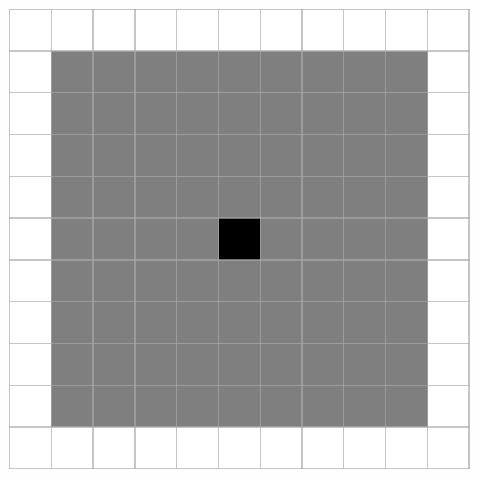
\includegraphics[width=\textwidth]{img/experimentacion/naturales/Flame3/vecindad_9x9.png}
			\caption{Vecindad de $9 \times 9$ (81 vecinos).}
			\label{fig:flame_vecindad_9x9}
		\end{subfigure}
		\hspace{1cm}
		\begin{subfigure}[b]{0.30\textwidth}
			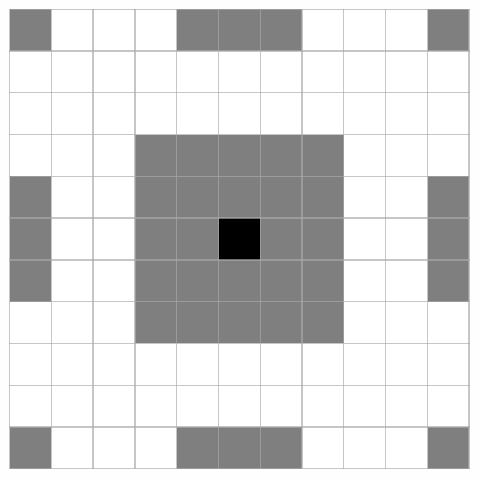
\includegraphics[width=\textwidth]{img/experimentacion/naturales/Flame3/vecindad_dispersa41.png}
			\caption{Vecindad dispersa (41 vecinos).}
			\label{fig:flame_vecindad_dispersa}
		\end{subfigure}
		\caption{Vecindades de las 18 configuraciones. La célula central, en negro, también es parte de la vecindad.}
		\label{fig:flame_vecindades}
	\end{figure}

	Todas las configuraciones se entrenaron durante 200 épocas con entropía cruzada como función de pérdida, una tasa de aprendizaje inicial de 0.001 con reducción exponencial hasta 0.00001, un tamaño del lote de 8,192, frontera abierta y semilla aleatoria 42. Para aprovechar todas las imágenes, con un paso de 30 s cada conjunto se divide en 6 secuencias que empiezan en imágenes distintas (0, 6, 12, \dots; 1, 7, 13, \dots; y así hasta 5, 11, 17, \dots) y las 6 se usan para entrenar; con un paso de 15 s se forman 3 secuencias y con uno de 5 s, solo una.

	Para comparar las configuraciones se usan cuatro medidas. Para el área quemada y el área con fuego, un valor de 100\% significa que la simulación libre es idéntica a la real. Para los dos errores, un valor de 100\% significa que la red se equivocó en la misma medida que la predicción sin cambio; menos de 100\% significa que la red es mejor y más de 100\%, que es peor. Por ejemplo, un error de 89\% indica que la red se equivoca 11\% menos que la predicción sin cambio, mientras que uno de 400\% indica que se equivoca cuatro veces más. 
	
	\begin{enumerate}
		\item El área quemada indica qué tanto se parece el área quemada al final de la simulación libre a la real.
		\item El área con fuego indica qué tanto se parecen las células que alguna vez llegaron a 130 °C.
		\item El error de un paso se mide prediciendo un solo paso desde cada imagen real.
		\item El error en la simulación libre se mide en su último paso.
	\end{enumerate} 

	Como de un paso a otro el fuego cambia pocas células, la predicción sin cambio tiene un error bajo y es difícil de superar; sin embargo, nunca propaga el fuego, por lo que su área quemada es de 0\%. Por esto, el área quemada indica si la red propaga el fuego hacia donde debe, y el error, si además acierta las temperaturas.

	Las configuraciones también se evaluaron de forma visual, eligiendo las mejores al ver la animación de la simulación libre junto a la evolución real (columna ``Selección visual''). Esta selección coincide con el área quemada: al probar en flame\_plot\_1 se eligieron las 5 primeras por área quemada, y al probar en flame\_plot\_2, la primera y la tercera. Esto indica que el área quemada es la medida que mejor representa si la simulación se parece a la propagación real. Las configuraciones elegidas de forma visual cumplen los siguientes criterios:
	
	\begin{itemize}
		\item Propagan el fuego a una velocidad constante y similar a la de la evolución de prueba.
		\item Si se inicia el sistema con una frontera periódica y con el fuego en el centro, los frentes de propagación del fuego se extinguen al colisionar.
		\item Una vez quemado todo el sistema, este ya no es capaz de generar fuego.
		\item El sistema se calienta y se enfría.
	\end{itemize}

	La tabla \ref{tab:flame_18_prueba1} muestra los resultados al probar en flame\_plot\_1. A diferencia de los experimentos sin estados de quemado, todas las configuraciones propagan el fuego: el área quemada se parece entre un 72 y un 86\% a la real. Las mejores son las redes de 2:32 y 3:64 con paso de 15 y 30 s, con un área quemada del 84 al 86\%. Sin embargo, ninguna supera a la predicción sin cambio en el error de la simulación libre: las de paso de 30 s se equivocan entre 1.4 y 2.3 veces más, y las de paso de 15 s, entre 3.6 y 4.5 veces más. Es decir, el fuego avanza hacia las zonas correctas, pero las temperaturas no coinciden con las reales.

	\begin{table}[htbp]
		\centering
		\footnotesize
		\setlength{\tabcolsep}{3pt}
		\begin{tabular}{@{}ccccccccc@{}}
			\toprule
			& & & & & & \textbf{Error en la} & & \\
			& & & & \textbf{Área} & \textbf{Área} & \textbf{simulación} & \textbf{Error de} & \textbf{Selección} \\
			\textbf{Lugar} & \textbf{Paso} & \textbf{Vecindad} & \textbf{Capas} & \textbf{quemada} & \textbf{con fuego} & \textbf{libre} & \textbf{un paso} & \textbf{visual} \\ \midrule
			1 & 15 s & Dispersa & 3:64 & 86\% & 68\% & 404\% & 113\% & $\checkmark$ \\
			2 & 30 s & Dispersa & 3:64 & 86\% & 67\% & 140\% & 119\% & $\checkmark$ \\
			3 & 30 s & $9 \times 9$ & 2:32 & 85\% & 55\% & 147\% & 110\% & $\checkmark$ \\
			4 & 15 s & $9 \times 9$ & 2:32 & 85\% & 57\% & 450\% & 108\% & $\checkmark$ \\
			5 & 15 s & $9 \times 9$ & 3:64 & 85\% & 68\% & 391\% & 118\% & $\checkmark$ \\
			6 & 30 s & Dispersa & 2:32 & 84\% & 67\% & 232\% & 114\% &  \\
			7 & 15 s & Dispersa & 2:32 & 84\% & 38\% & 364\% & 106\% &  \\
			8 & 30 s & $9 \times 9$ & 3:64 & 84\% & 65\% & 170\% & 125\% & $\checkmark$ \\
			9 & 5 s & Dispersa & 4:256 & 83\% & 69\% & 709\% & 119\% &  \\
			10 & 5 s & $9 \times 9$ & 4:256 & 79\% & 69\% & 429\% & 126\% &  \\
			11 & 15 s & $9 \times 9$ & 4:256 & 79\% & 68\% & 326\% & 145\% &  \\
			12 & 15 s & Dispersa & 4:256 & 78\% & 68\% & 287\% & 140\% & $\checkmark$ \\
			% 13 & 5 s & $9 \times 9$ & 2:32 & 74\% & 71\% & 1203\% & 102\% &  \\
			% 14 & 30 s & Dispersa & 4:256 & 74\% & 67\% & 382\% & 145\% &  \\
			% 15 & 5 s & Dispersa & 3:64 & 74\% & 69\% & 1179\% & 102\% &  \\
			% 16 & 30 s & $9 \times 9$ & 4:256 & 73\% & 66\% & 471\% & 148\% &  \\
			% 17 & 5 s & $9 \times 9$ & 3:64 & 73\% & 69\% & 909\% & 107\% &  \\
			% 18 & 5 s & Dispersa & 2:32 & 72\% & 70\% & 1195\% & 101\% &  \\
			\bottomrule
		\end{tabular}
		\caption{Las 12 mejores configuraciones probadas en flame\_plot\_1 y entrenadas con flame\_plot\_2, ordenadas por área quemada.}
		\label{tab:flame_18_prueba1}
	\end{table}

	

	La tabla \ref{tab:flame_18_prueba2} muestra los resultados al probar en flame\_plot\_2, en donde el fuego es más difícil de reproducir: el área quemada se parece como máximo en un 67\% a la real. En este caso las mejores son las redes de 4:256, ya que las redes de 2:32 propagan el fuego muy lento y su área quemada se queda entre el 10 y el 30\%. En esta prueba varias configuraciones sí superan a la predicción sin cambio en la simulación libre, como la de $9 \times 9$ con 4:256 y paso de 15 s, que tiene el área quemada más parecida (67\%) y se equivoca un 11\% menos que la predicción sin cambio.


	\begin{table}[htbp]
		\centering
		\footnotesize
		\setlength{\tabcolsep}{3pt}
		\begin{tabular}{@{}ccccccccc@{}}
			\toprule
			& & & & & & \textbf{Error en la} & & \\
			& & & & \textbf{Área} & \textbf{Área} & \textbf{simulación} & \textbf{Error de} & \textbf{Selección} \\
			\textbf{Lugar} & \textbf{Paso} & \textbf{Vecindad} & \textbf{Capas} & \textbf{quemada} & \textbf{con fuego} & \textbf{libre} & \textbf{un paso} & \textbf{visual} \\ \midrule
			1 & 15 s & $9 \times 9$ & 4:256 & 67\% & 61\% & 89\% & 105\% & $\checkmark$ \\
			2 & 5 s & Dispersa & 4:256 & 61\% & 52\% & 77\% & 117\% &  \\
			3 & 5 s & $9 \times 9$ & 4:256 & 57\% & 44\% & 87\% & 118\% & $\checkmark$ \\
			4 & 15 s & Dispersa & 4:256 & 50\% & 44\% & 94\% & 104\% &  \\
			5 & 30 s & $9 \times 9$ & 4:256 & 49\% & 44\% & 96\% & 93\% &  \\
			6 & 15 s & $9 \times 9$ & 3:64 & 43\% & 41\% & 99\% & 104\% &  \\
			7 & 15 s & Dispersa & 3:64 & 40\% & 40\% & 112\% & 100\% &  \\
			8 & 30 s & Dispersa & 4:256 & 39\% & 34\% & 94\% & 92\% &  \\
			9 & 30 s & $9 \times 9$ & 3:64 & 36\% & 33\% & 102\% & 93\% &  \\
			10 & 30 s & Dispersa & 3:64 & 33\% & 29\% & 101\% & 90\% &  \\
			11 & 30 s & $9 \times 9$ & 2:32 & 30\% & 27\% & 97\% & 89\% &  \\
			12 & 5 s & $9 \times 9$ & 3:64 & 28\% & 27\% & 126\% & 110\% &  \\
			% 13 & 30 s & Dispersa & 2:32 & 25\% & 20\% & 97\% & 88\% &  \\
			% 14 & 15 s & $9 \times 9$ & 2:32 & 23\% & 19\% & 98\% & 101\% &  \\
			% 15 & 15 s & Dispersa & 2:32 & 22\% & 21\% & 107\% & 101\% &  \\
			% 16 & 5 s & Dispersa & 3:64 & 21\% & 21\% & 129\% & 106\% &  \\
			% 17 & 5 s & $9 \times 9$ & 2:32 & 16\% & 23\% & 149\% & 108\% &  \\
			% 18 & 5 s & Dispersa & 2:32 & 10\% & 28\% & 173\% & 104\% &  \\
			\bottomrule
		\end{tabular}
		\caption{Las 12 mejores configuraciones probadas en flame\_plot\_2 y entrenadas con flame\_plot\_1, ordenadas por área quemada.}
		\label{tab:flame_18_prueba2}
	\end{table}

	
	Ninguna configuración es la mejor en las dos pruebas: las redes chicas funcionan mejor en flame\_plot\_1 y las grandes en flame\_plot\_2. Para elegir una configuración general, en la tabla \ref{tab:flame_18_lugares} se ordenan las configuraciones de la 1 (mejor) a la 18 en cada prueba y se promedia su lugar. Considerando solo el área quemada, las mejores son la dispersa con 3:64 y paso de 15 s, la de $9 \times 9$ con 3:64 y paso de 15 s, y la dispersa con 4:256 y paso de 5 s. Considerando las cuatro medidas (lugar combinado), las mejores son la dispersa con 3:64 y paso de 15 o 30 s, y la de $9 \times 9$ con 2:32 y paso de 30 s. En ambos casos, las peores son las de paso de 5 s con redes de 2:32 o 3:64: las células quemadas no se enfrían y el error en la simulación libre llega a ser 12 veces el de la predicción sin cambio.

	\begin{table}[htbp]
		\centering
		\footnotesize
		\setlength{\tabcolsep}{3pt}
		\begin{tabular}{ccccccccc}
			\toprule
			& & & \multicolumn{3}{c}{\textbf{Lugar por área quemada}} & \multicolumn{3}{c}{\textbf{Lugar combinado}} \\
			\cmidrule(lr){4-6} \cmidrule(lr){7-9}
			& & & \textbf{Prueba} & \textbf{Prueba} & & \textbf{Prueba} & \textbf{Prueba} & \\
			\textbf{Paso} & \textbf{Vecindad} & \textbf{Capas} & \textbf{1} & \textbf{2} & \textbf{Promedio} & \textbf{1} & \textbf{2} & \textbf{Promedio} \\ \midrule
			15 s & Dispersa & 3:64 & 1 & 7 & 4 & 1 & 10 & 5.5 \\
			15 s & $9 \times 9$ & 3:64 & 5 & 6 & 5.5 & 5 & 7 & 6 \\
			5 s & Dispersa & 4:256 & 9 & 2 & 5.5 & 9.5 & 3 & 6.25 \\
			30 s & Dispersa & 3:64 & 2 & 10 & 6 & 2 & 9 & 5.5 \\
			15 s & $9 \times 9$ & 4:256 & 11 & 1 & 6 & 14 & 1 & 7.5 \\
			5 s & $9 \times 9$ & 4:256 & 10 & 3 & 6.5 & 9.5 & 6 & 7.75 \\
			30 s & $9 \times 9$ & 2:32 & 3 & 11 & 7 & 3 & 8 & 5.5 \\
			15 s & Dispersa & 4:256 & 12 & 4 & 8 & 15.5 & 4.5 & 10 \\
			30 s & $9 \times 9$ & 3:64 & 8 & 9 & 8.5 & 12 & 11 & 11.5 \\
			15 s & $9 \times 9$ & 2:32 & 4 & 14 & 9 & 9.5 & 13 & 11.25 \\
			30 s & Dispersa & 2:32 & 6 & 13 & 9.5 & 4 & 12 & 8 \\
			30 s & $9 \times 9$ & 4:256 & 16 & 5 & 10.5 & 18 & 2 & 10 \\
			15 s & Dispersa & 2:32 & 7 & 15 & 11 & 7 & 14 & 10.5 \\
			30 s & Dispersa & 4:256 & 14 & 8 & 11 & 17 & 4.5 & 10.75 \\
			5 s & $9 \times 9$ & 3:64 & 17 & 12 & 14.5 & 15.5 & 15 & 15.25 \\
			5 s & $9 \times 9$ & 2:32 & 13 & 17 & 15 & 6 & 18 & 12 \\
			5 s & Dispersa & 3:64 & 15 & 16 & 15.5 & 13 & 17 & 15 \\
			5 s & Dispersa & 2:32 & 18 & 18 & 18 & 9.5 & 16 & 12.75 \\ \bottomrule
		\end{tabular}
		\caption{Lugar de cada configuración (1 = mejor) entre las 18, ordenadas por el promedio del lugar por área quemada.}
		\label{tab:flame_18_lugares}
	\end{table}

	Las tres configuraciones con mejor lugar combinado empatan con 5.5. De ellas, se elige como configuración final la de paso de 30 s, vecindad de $9 \times 9$ y 2:32:ReLU, por ser la red más pequeña y la única de las tres que, al probar en flame\_plot\_2, se equivoca menos que la predicción sin cambio tanto en un paso (89\%) como en la simulación libre (97\%).

	La figura \ref{fig:flame_criterios} muestra la configuración final en el simulador con los criterios de la selección visual. El espacio inicia frío y sin quemar, con un foco de fuego en el centro y frontera periódica: el fuego se propaga en todas direcciones (b y c), los frentes se extinguen al encontrarse después de cruzar la frontera (d y e) y, una vez quemado todo el espacio, ya no vuelve a aparecer fuego (f).

	% Leyenda de los 18 estados con la paleta del simulador (Simulator/GUI/colores/flame_log12_quemado6.csv)
	\definecolor{flame0}{HTML}{448CFD}\definecolor{flame1}{HTML}{17D9C7}\definecolor{flame2}{HTML}{2FF09A}
	\definecolor{flame3}{HTML}{69FD65}\definecolor{flame4}{HTML}{A1FC3D}\definecolor{flame5}{HTML}{CDEB34}
	\definecolor{flame6}{HTML}{EDCF39}\definecolor{flame7}{HTML}{FDA932}\definecolor{flame8}{HTML}{FA7A1F}
	\definecolor{flame9}{HTML}{E84B0C}\definecolor{flame10}{HTML}{CB2B03}\definecolor{flame11}{HTML}{A01101}
	\definecolor{flame12}{HTML}{000000}\definecolor{flame13}{HTML}{333333}\definecolor{flame14}{HTML}{666666}
	\definecolor{flame15}{HTML}{999999}\definecolor{flame16}{HTML}{CCCCCC}\definecolor{flame17}{HTML}{FFFFFF}
	\newcommand{\estadoflame}[2][black]{\fcolorbox{gray}{flame#2}{\makebox[1.1em]{\textcolor{#1}{#2}}}}
	\newcommand{\leyendaflame}{%
		\par\medskip
		{\footnotesize\setlength{\fboxsep}{1pt}%
		Temperatura: \estadoflame{0}\estadoflame{1}\estadoflame{2}\estadoflame{3}\estadoflame{4}\estadoflame{5}%
		\estadoflame{6}\estadoflame{7}\estadoflame{8}\estadoflame{9}\estadoflame[white]{10}\estadoflame[white]{11}%
		\quad Quemado: \estadoflame[white]{12}\estadoflame[white]{13}\estadoflame[white]{14}\estadoflame{15}%
		\estadoflame{16}\estadoflame{17}\par}}

	\begin{figure}[htbp]
		\centering
		\begin{subfigure}[t]{0.3\textwidth}
			\centering
			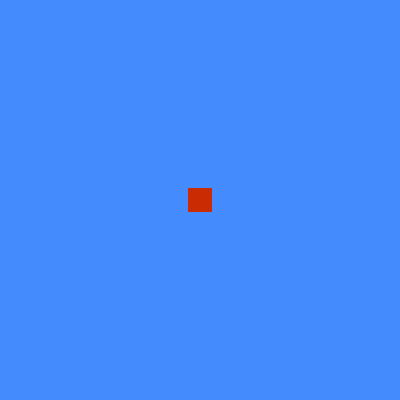
\includegraphics[width=\linewidth]{img/experimentacion/naturales/Flame3/criterios/entrenada_flame_plot_2/paso_0.png}
			\caption{0 s}
			\label{fig:flame_criterios_0s}
		\end{subfigure}
		\hfill
		\begin{subfigure}[t]{0.3\textwidth}
			\centering
			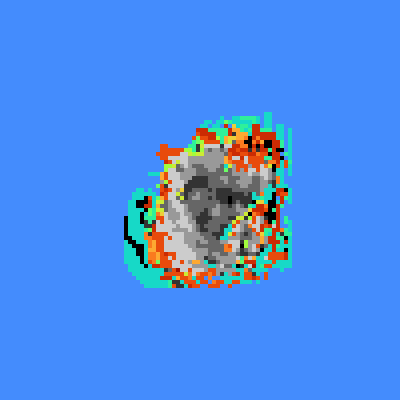
\includegraphics[width=\linewidth]{img/experimentacion/naturales/Flame3/criterios/entrenada_flame_plot_2/paso_5.png}
			\caption{150 s}
			\label{fig:flame_criterios_150s}
		\end{subfigure}
		\hfill
		\begin{subfigure}[t]{0.3\textwidth}
			\centering
			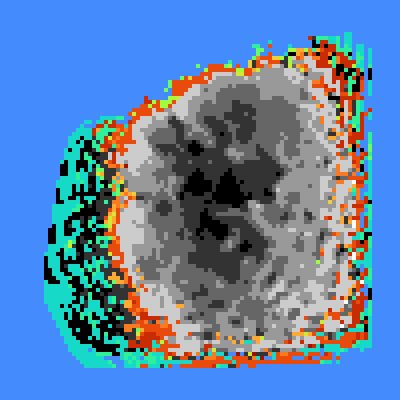
\includegraphics[width=\linewidth]{img/experimentacion/naturales/Flame3/criterios/entrenada_flame_plot_2/paso_10.png}
			\caption{300 s}
			\label{fig:flame_criterios_300s}
		\end{subfigure}
		\\[6pt]
		\begin{subfigure}[t]{0.3\textwidth}
			\centering
			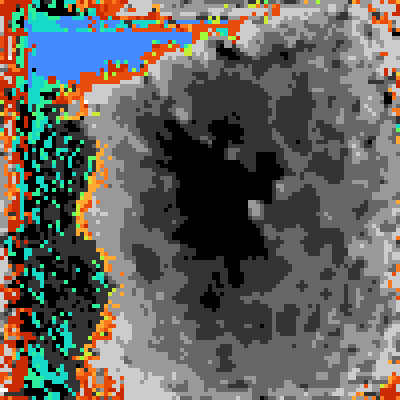
\includegraphics[width=\linewidth]{img/experimentacion/naturales/Flame3/criterios/entrenada_flame_plot_2/paso_14.png}
			\caption{420 s}
			\label{fig:flame_criterios_420s}
		\end{subfigure}
		\hfill
		\begin{subfigure}[t]{0.3\textwidth}
			\centering
			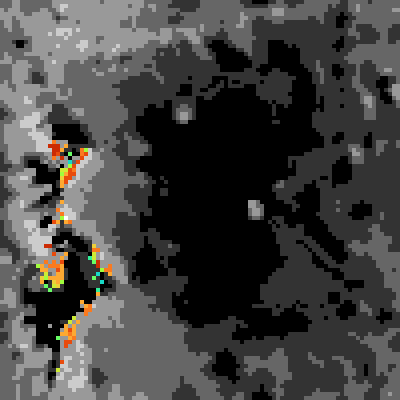
\includegraphics[width=\linewidth]{img/experimentacion/naturales/Flame3/criterios/entrenada_flame_plot_2/paso_18.png}
			\caption{540 s}
			\label{fig:flame_criterios_540s}
		\end{subfigure}
		\hfill
		\begin{subfigure}[t]{0.3\textwidth}
			\centering
			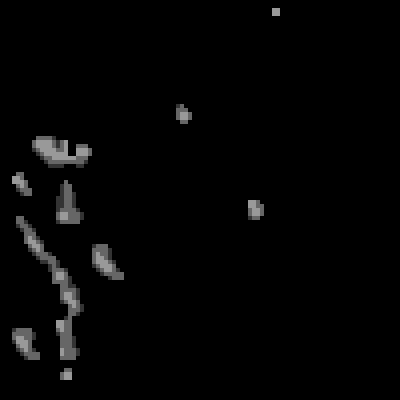
\includegraphics[width=\linewidth]{img/experimentacion/naturales/Flame3/criterios/entrenada_flame_plot_2/paso_40.png}
			\caption{1200 s}
			\label{fig:flame_criterios_1200s}
		\end{subfigure}
		\leyendaflame
		\caption{Configuración final (paso de 30 s, vecindad de $9 \times 9$ y 2:32:ReLU, entrenada con flame\_plot\_2) en el simulador, con frontera periódica. El espacio de $100 \times 100$ células inicia en el estado 0 con un foco de $6 \times 6$ células en el estado 10 en el centro. Los colores son los estados de la tabla \ref{tab:flame_states_proportion}.}
		\label{fig:flame_criterios}
	\end{figure}

	En las figuras \ref{fig:flame_comparacion1} y \ref{fig:flame_comparacion2} se muestran la evolución original y la comparativa con las 9 configuraciones de la selección visual de ambas pruebas, al probar en flame\_plot\_1 y en flame\_plot\_2, respectivamente.

	\begin{figure}[htbp]
		\centering
		\begin{subfigure}[t]{0.48\textwidth}
			\centering
			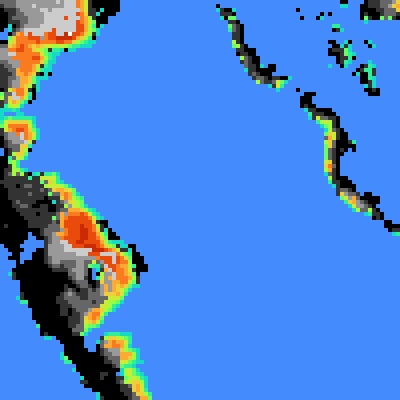
\includegraphics[width=0.32\linewidth]{img/experimentacion/naturales/Flame3/comparacion/flame_plot_1/real_150s.png}\hfill
			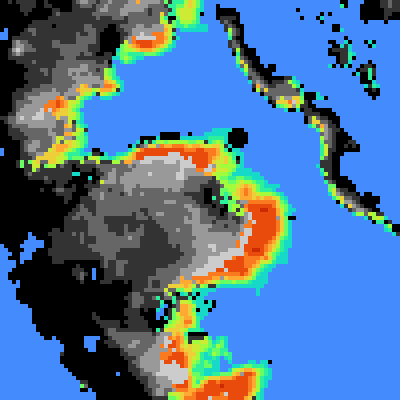
\includegraphics[width=0.32\linewidth]{img/experimentacion/naturales/Flame3/comparacion/flame_plot_1/real_300s.png}\hfill
			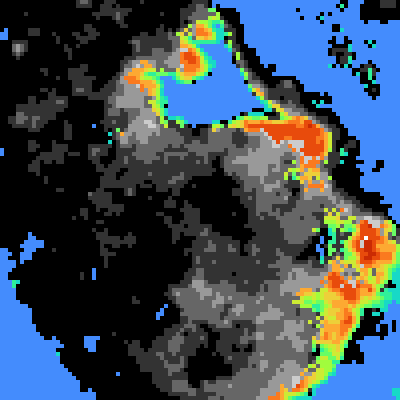
\includegraphics[width=0.32\linewidth]{img/experimentacion/naturales/Flame3/comparacion/flame_plot_1/real_420s.png}
			\caption{Real}
			\label{fig:flame_comparacion1_real}
		\end{subfigure}
		\hfill
		\begin{subfigure}[t]{0.48\textwidth}
			\centering
			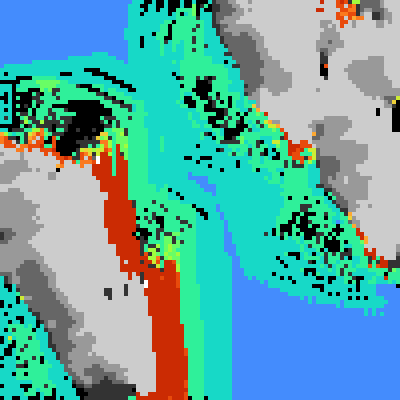
\includegraphics[width=0.32\linewidth]{img/experimentacion/naturales/Flame3/comparacion/flame_plot_1/paso15s_9x9_2x32_150s.png}\hfill
			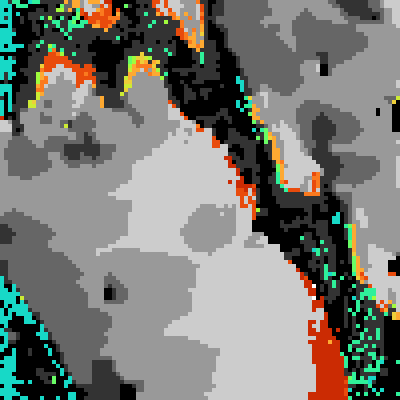
\includegraphics[width=0.32\linewidth]{img/experimentacion/naturales/Flame3/comparacion/flame_plot_1/paso15s_9x9_2x32_300s.png}\hfill
			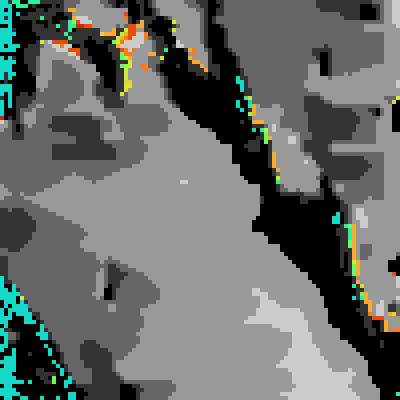
\includegraphics[width=0.32\linewidth]{img/experimentacion/naturales/Flame3/comparacion/flame_plot_1/paso15s_9x9_2x32_420s.png}
			\caption{15 s, $9 \times 9$, 2:32}
			\label{fig:flame_comparacion1_paso15s_9x9_2x32}
		\end{subfigure}
		\\[6pt]
		\begin{subfigure}[t]{0.48\textwidth}
			\centering
			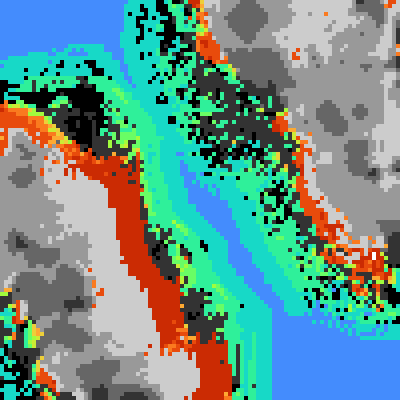
\includegraphics[width=0.32\linewidth]{img/experimentacion/naturales/Flame3/comparacion/flame_plot_1/paso15s_9x9_3x64_150s.png}\hfill
			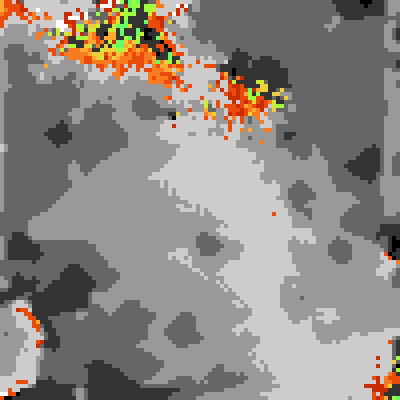
\includegraphics[width=0.32\linewidth]{img/experimentacion/naturales/Flame3/comparacion/flame_plot_1/paso15s_9x9_3x64_300s.png}\hfill
			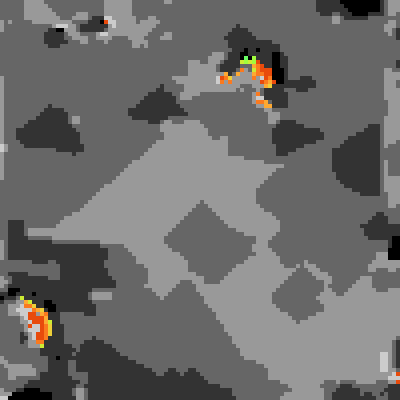
\includegraphics[width=0.32\linewidth]{img/experimentacion/naturales/Flame3/comparacion/flame_plot_1/paso15s_9x9_3x64_420s.png}
			\caption{15 s, $9 \times 9$, 3:64}
			\label{fig:flame_comparacion1_paso15s_9x9_3x64}
		\end{subfigure}
		\hfill
		\begin{subfigure}[t]{0.48\textwidth}
			\centering
			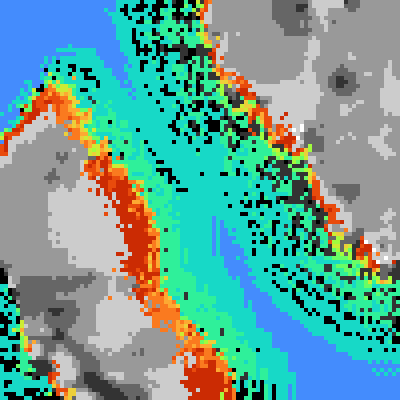
\includegraphics[width=0.32\linewidth]{img/experimentacion/naturales/Flame3/comparacion/flame_plot_1/paso15s_dispersa41_3x64_150s.png}\hfill
			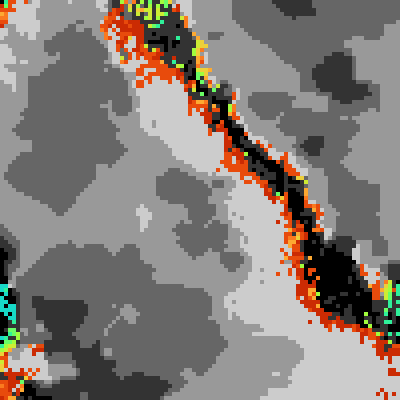
\includegraphics[width=0.32\linewidth]{img/experimentacion/naturales/Flame3/comparacion/flame_plot_1/paso15s_dispersa41_3x64_300s.png}\hfill
			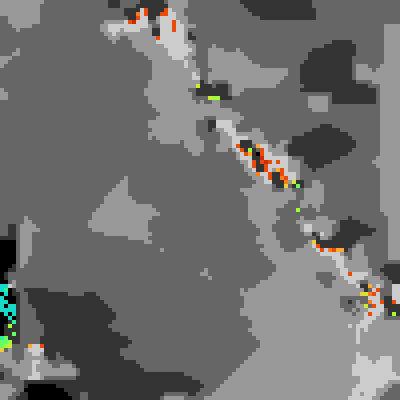
\includegraphics[width=0.32\linewidth]{img/experimentacion/naturales/Flame3/comparacion/flame_plot_1/paso15s_dispersa41_3x64_420s.png}
			\caption{15 s, dispersa, 3:64}
			\label{fig:flame_comparacion1_paso15s_dispersa41_3x64}
		\end{subfigure}
		\\[6pt]
		\begin{subfigure}[t]{0.48\textwidth}
			\centering
			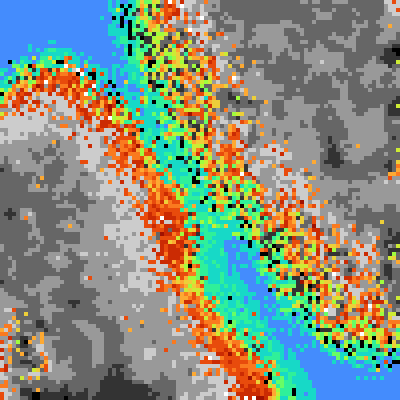
\includegraphics[width=0.32\linewidth]{img/experimentacion/naturales/Flame3/comparacion/flame_plot_1/paso15s_dispersa41_4x256_150s.png}\hfill
			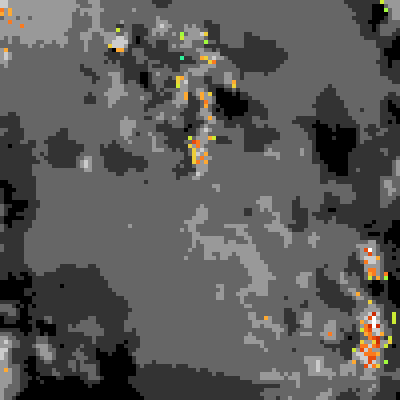
\includegraphics[width=0.32\linewidth]{img/experimentacion/naturales/Flame3/comparacion/flame_plot_1/paso15s_dispersa41_4x256_300s.png}\hfill
			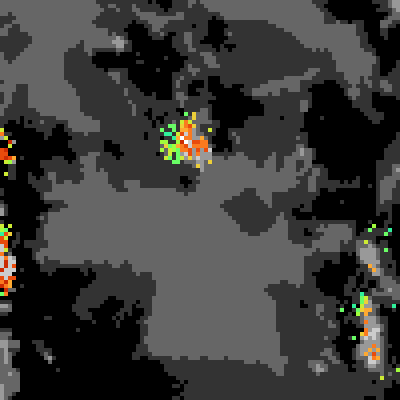
\includegraphics[width=0.32\linewidth]{img/experimentacion/naturales/Flame3/comparacion/flame_plot_1/paso15s_dispersa41_4x256_420s.png}
			\caption{15 s, dispersa, 4:256}
			\label{fig:flame_comparacion1_paso15s_dispersa41_4x256}
		\end{subfigure}
		\hfill
		\begin{subfigure}[t]{0.48\textwidth}
			\centering
			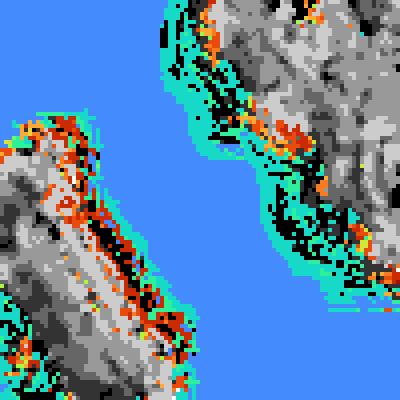
\includegraphics[width=0.32\linewidth]{img/experimentacion/naturales/Flame3/comparacion/flame_plot_1/paso30s_9x9_2x32_150s.png}\hfill
			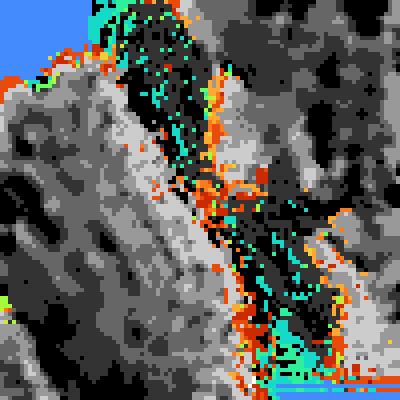
\includegraphics[width=0.32\linewidth]{img/experimentacion/naturales/Flame3/comparacion/flame_plot_1/paso30s_9x9_2x32_300s.png}\hfill
			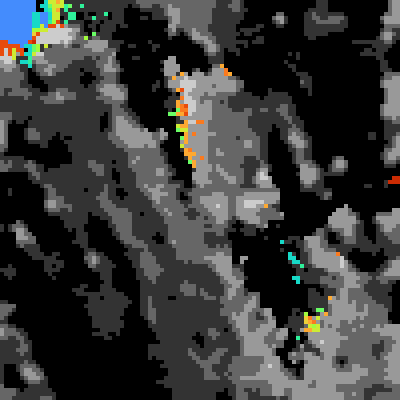
\includegraphics[width=0.32\linewidth]{img/experimentacion/naturales/Flame3/comparacion/flame_plot_1/paso30s_9x9_2x32_420s.png}
			\caption{30 s, $9 \times 9$, 2:32}
			\label{fig:flame_comparacion1_paso30s_9x9_2x32}
		\end{subfigure}
		\\[6pt]
		\begin{subfigure}[t]{0.48\textwidth}
			\centering
			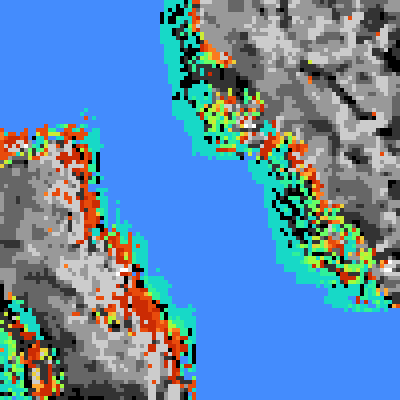
\includegraphics[width=0.32\linewidth]{img/experimentacion/naturales/Flame3/comparacion/flame_plot_1/paso30s_9x9_3x64_150s.png}\hfill
			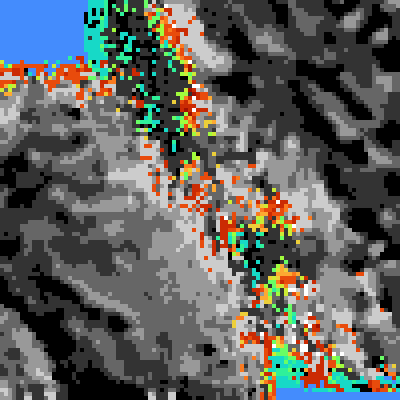
\includegraphics[width=0.32\linewidth]{img/experimentacion/naturales/Flame3/comparacion/flame_plot_1/paso30s_9x9_3x64_300s.png}\hfill
			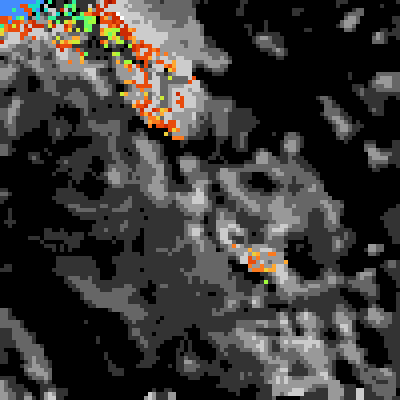
\includegraphics[width=0.32\linewidth]{img/experimentacion/naturales/Flame3/comparacion/flame_plot_1/paso30s_9x9_3x64_420s.png}
			\caption{30 s, $9 \times 9$, 3:64}
			\label{fig:flame_comparacion1_paso30s_9x9_3x64}
		\end{subfigure}
		\hfill
		\begin{subfigure}[t]{0.48\textwidth}
			\centering
			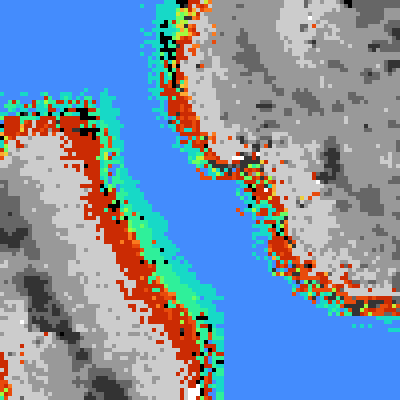
\includegraphics[width=0.32\linewidth]{img/experimentacion/naturales/Flame3/comparacion/flame_plot_1/paso30s_dispersa41_3x64_150s.png}\hfill
			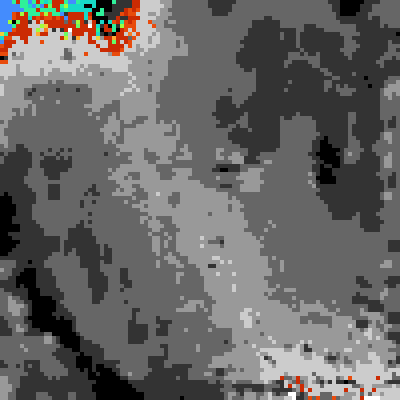
\includegraphics[width=0.32\linewidth]{img/experimentacion/naturales/Flame3/comparacion/flame_plot_1/paso30s_dispersa41_3x64_300s.png}\hfill
			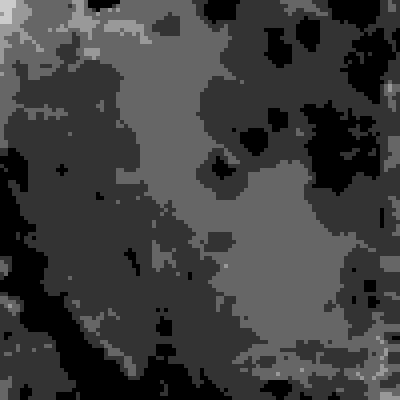
\includegraphics[width=0.32\linewidth]{img/experimentacion/naturales/Flame3/comparacion/flame_plot_1/paso30s_dispersa41_3x64_420s.png}
			\caption{30 s, dispersa, 3:64}
			\label{fig:flame_comparacion1_paso30s_dispersa41_3x64}
		\end{subfigure}
		\\[6pt]
		\begin{subfigure}[t]{0.48\textwidth}
			\centering
			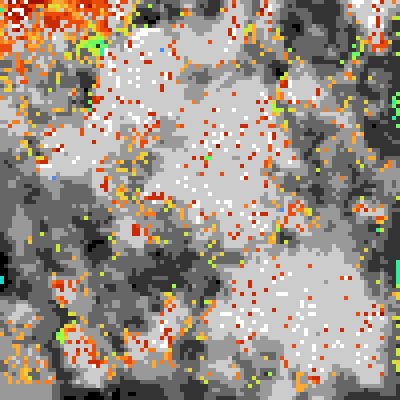
\includegraphics[width=0.32\linewidth]{img/experimentacion/naturales/Flame3/comparacion/flame_plot_1/paso5s_9x9_4x256_150s.png}\hfill
			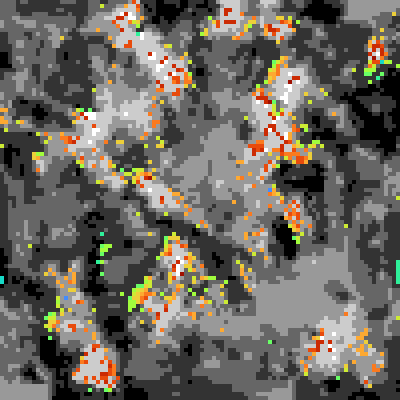
\includegraphics[width=0.32\linewidth]{img/experimentacion/naturales/Flame3/comparacion/flame_plot_1/paso5s_9x9_4x256_300s.png}\hfill
			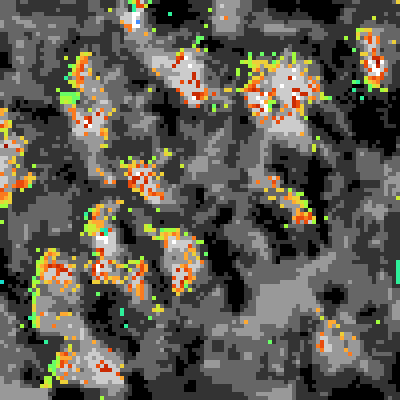
\includegraphics[width=0.32\linewidth]{img/experimentacion/naturales/Flame3/comparacion/flame_plot_1/paso5s_9x9_4x256_420s.png}
			\caption{5 s, $9 \times 9$, 4:256}
			\label{fig:flame_comparacion1_paso5s_9x9_4x256}
		\end{subfigure}
		\hfill
		\begin{subfigure}[t]{0.48\textwidth}
			\centering
			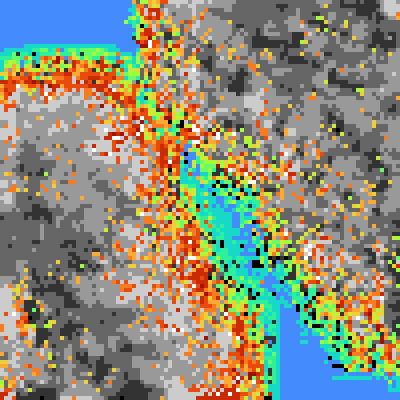
\includegraphics[width=0.32\linewidth]{img/experimentacion/naturales/Flame3/comparacion/flame_plot_1/paso15s_9x9_4x256_150s.png}\hfill
			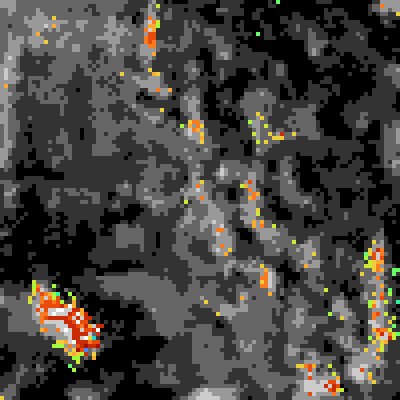
\includegraphics[width=0.32\linewidth]{img/experimentacion/naturales/Flame3/comparacion/flame_plot_1/paso15s_9x9_4x256_300s.png}\hfill
			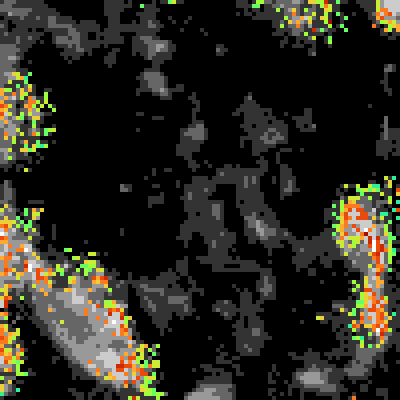
\includegraphics[width=0.32\linewidth]{img/experimentacion/naturales/Flame3/comparacion/flame_plot_1/paso15s_9x9_4x256_420s.png}
			\caption{15 s, $9 \times 9$, 4:256}
			\label{fig:flame_comparacion1_paso15s_9x9_4x256}
		\end{subfigure}
		\leyendaflame
		\caption{Evolución de flame\_plot\_1 (a) y simulación libre de las 9 configuraciones de ambas pruebas, entrenadas con flame\_plot\_2. En cada una: 150, 300 y 420 s después de la imagen inicial.}
		\label{fig:flame_comparacion1}
	\end{figure}

	\begin{figure}[htbp]
		\centering
		\begin{subfigure}[t]{0.48\textwidth}
			\centering
			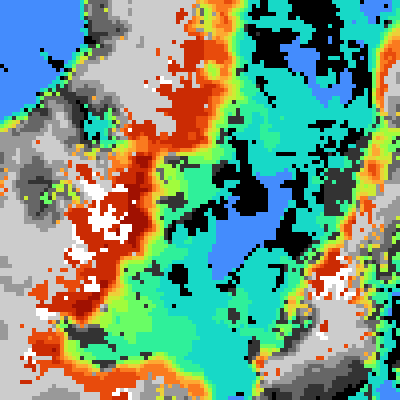
\includegraphics[width=0.32\linewidth]{img/experimentacion/naturales/Flame3/comparacion/flame_plot_2/real_90s.png}\hfill
			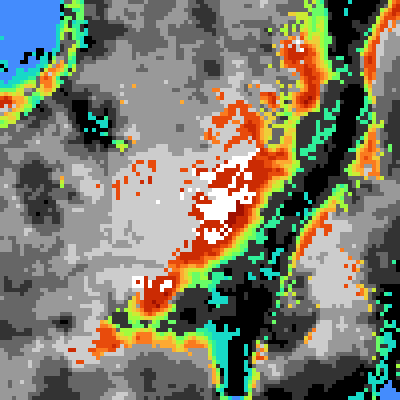
\includegraphics[width=0.32\linewidth]{img/experimentacion/naturales/Flame3/comparacion/flame_plot_2/real_150s.png}\hfill
			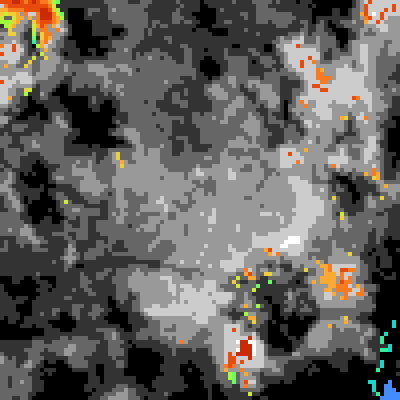
\includegraphics[width=0.32\linewidth]{img/experimentacion/naturales/Flame3/comparacion/flame_plot_2/real_240s.png}
			\caption{Real}
			\label{fig:flame_comparacion2_real}
		\end{subfigure}
		\hfill
		\begin{subfigure}[t]{0.48\textwidth}
			\centering
			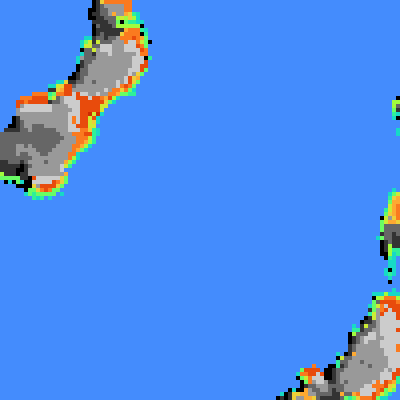
\includegraphics[width=0.32\linewidth]{img/experimentacion/naturales/Flame3/comparacion/flame_plot_2/paso15s_9x9_2x32_90s.png}\hfill
			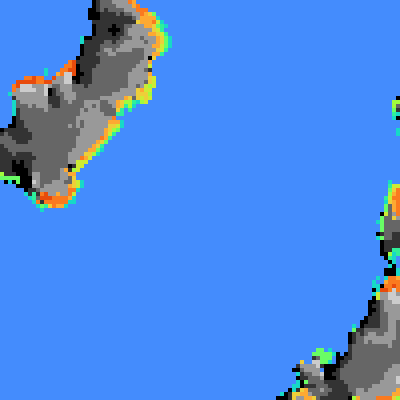
\includegraphics[width=0.32\linewidth]{img/experimentacion/naturales/Flame3/comparacion/flame_plot_2/paso15s_9x9_2x32_150s.png}\hfill
			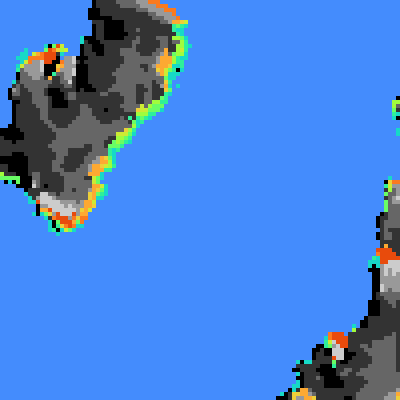
\includegraphics[width=0.32\linewidth]{img/experimentacion/naturales/Flame3/comparacion/flame_plot_2/paso15s_9x9_2x32_240s.png}
			\caption{15 s, $9 \times 9$, 2:32}
			\label{fig:flame_comparacion2_paso15s_9x9_2x32}
		\end{subfigure}
		\\[6pt]
		\begin{subfigure}[t]{0.48\textwidth}
			\centering
			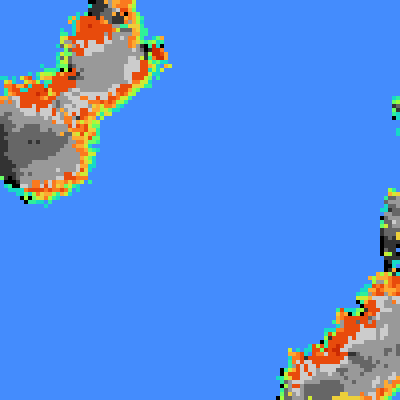
\includegraphics[width=0.32\linewidth]{img/experimentacion/naturales/Flame3/comparacion/flame_plot_2/paso15s_9x9_3x64_90s.png}\hfill
			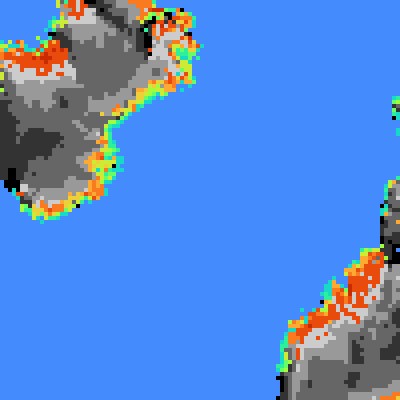
\includegraphics[width=0.32\linewidth]{img/experimentacion/naturales/Flame3/comparacion/flame_plot_2/paso15s_9x9_3x64_150s.png}\hfill
			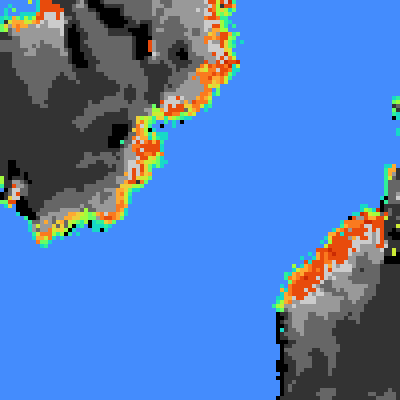
\includegraphics[width=0.32\linewidth]{img/experimentacion/naturales/Flame3/comparacion/flame_plot_2/paso15s_9x9_3x64_240s.png}
			\caption{15 s, $9 \times 9$, 3:64}
			\label{fig:flame_comparacion2_paso15s_9x9_3x64}
		\end{subfigure}
		\hfill
		\begin{subfigure}[t]{0.48\textwidth}
			\centering
			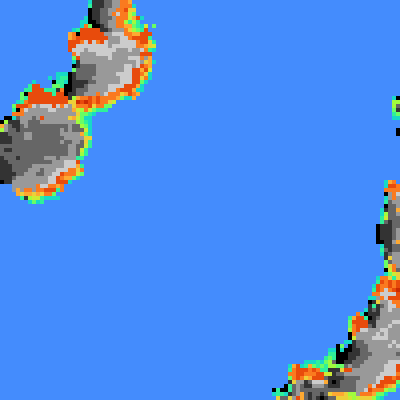
\includegraphics[width=0.32\linewidth]{img/experimentacion/naturales/Flame3/comparacion/flame_plot_2/paso15s_dispersa41_3x64_90s.png}\hfill
			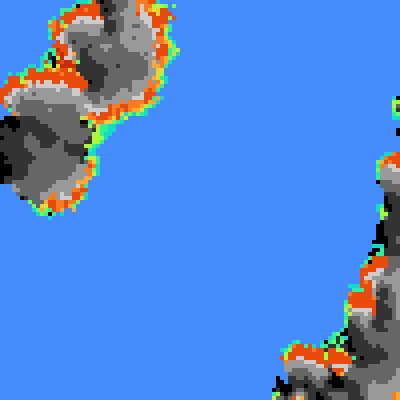
\includegraphics[width=0.32\linewidth]{img/experimentacion/naturales/Flame3/comparacion/flame_plot_2/paso15s_dispersa41_3x64_150s.png}\hfill
			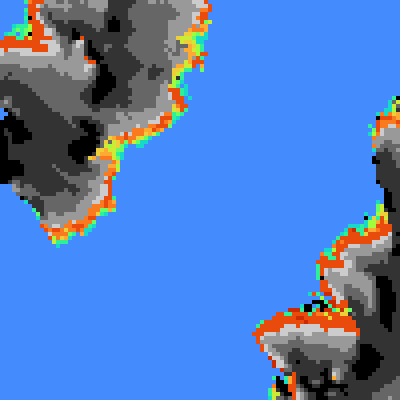
\includegraphics[width=0.32\linewidth]{img/experimentacion/naturales/Flame3/comparacion/flame_plot_2/paso15s_dispersa41_3x64_240s.png}
			\caption{15 s, dispersa, 3:64}
			\label{fig:flame_comparacion2_paso15s_dispersa41_3x64}
		\end{subfigure}
		\\[6pt]
		\begin{subfigure}[t]{0.48\textwidth}
			\centering
			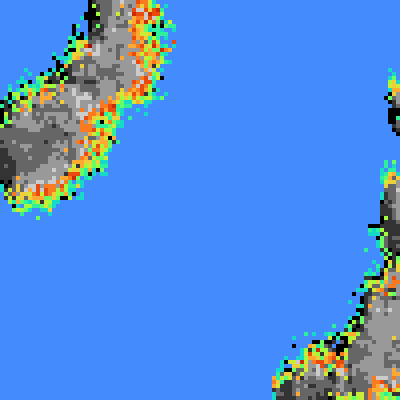
\includegraphics[width=0.32\linewidth]{img/experimentacion/naturales/Flame3/comparacion/flame_plot_2/paso15s_dispersa41_4x256_90s.png}\hfill
			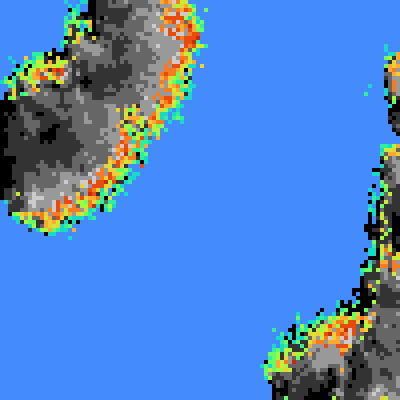
\includegraphics[width=0.32\linewidth]{img/experimentacion/naturales/Flame3/comparacion/flame_plot_2/paso15s_dispersa41_4x256_150s.png}\hfill
			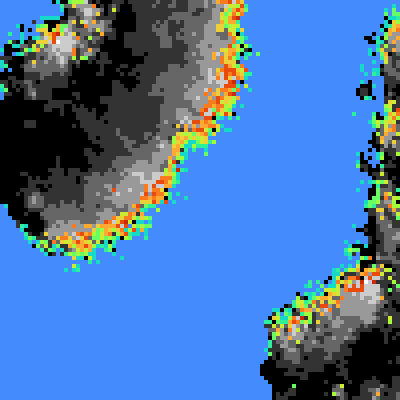
\includegraphics[width=0.32\linewidth]{img/experimentacion/naturales/Flame3/comparacion/flame_plot_2/paso15s_dispersa41_4x256_240s.png}
			\caption{15 s, dispersa, 4:256}
			\label{fig:flame_comparacion2_paso15s_dispersa41_4x256}
		\end{subfigure}
		\hfill
		\begin{subfigure}[t]{0.48\textwidth}
			\centering
			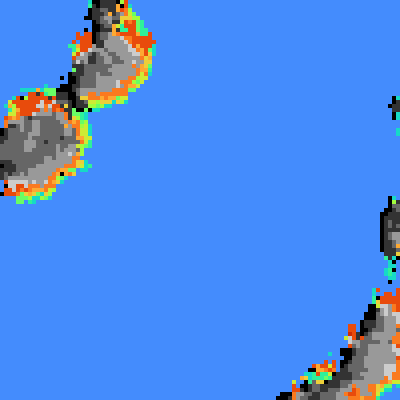
\includegraphics[width=0.32\linewidth]{img/experimentacion/naturales/Flame3/comparacion/flame_plot_2/paso30s_9x9_2x32_90s.png}\hfill
			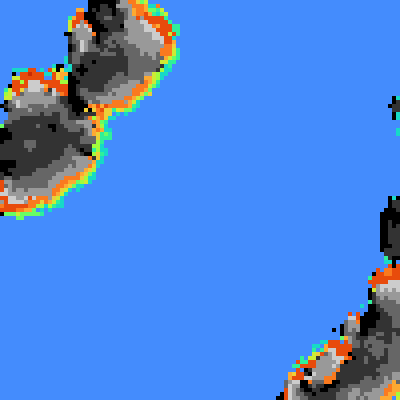
\includegraphics[width=0.32\linewidth]{img/experimentacion/naturales/Flame3/comparacion/flame_plot_2/paso30s_9x9_2x32_150s.png}\hfill
			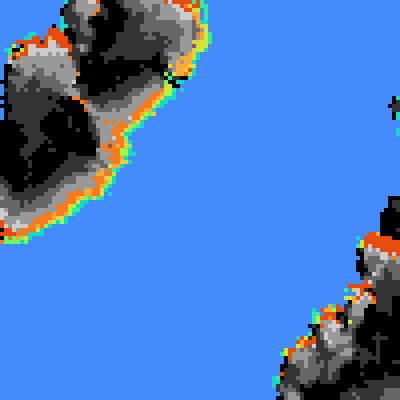
\includegraphics[width=0.32\linewidth]{img/experimentacion/naturales/Flame3/comparacion/flame_plot_2/paso30s_9x9_2x32_240s.png}
			\caption{30 s, $9 \times 9$, 2:32}
			\label{fig:flame_comparacion2_paso30s_9x9_2x32}
		\end{subfigure}
		\\[6pt]
		\begin{subfigure}[t]{0.48\textwidth}
			\centering
			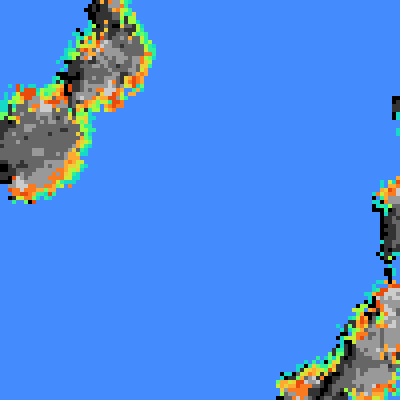
\includegraphics[width=0.32\linewidth]{img/experimentacion/naturales/Flame3/comparacion/flame_plot_2/paso30s_9x9_3x64_90s.png}\hfill
			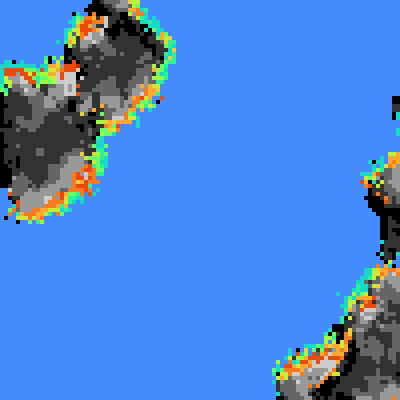
\includegraphics[width=0.32\linewidth]{img/experimentacion/naturales/Flame3/comparacion/flame_plot_2/paso30s_9x9_3x64_150s.png}\hfill
			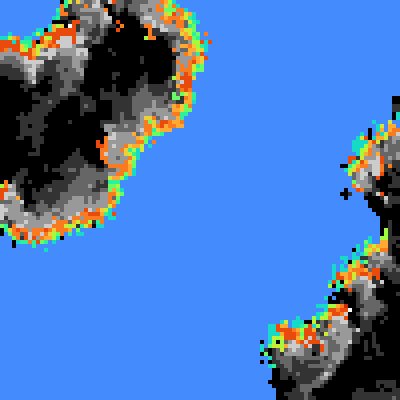
\includegraphics[width=0.32\linewidth]{img/experimentacion/naturales/Flame3/comparacion/flame_plot_2/paso30s_9x9_3x64_240s.png}
			\caption{30 s, $9 \times 9$, 3:64}
			\label{fig:flame_comparacion2_paso30s_9x9_3x64}
		\end{subfigure}
		\hfill
		\begin{subfigure}[t]{0.48\textwidth}
			\centering
			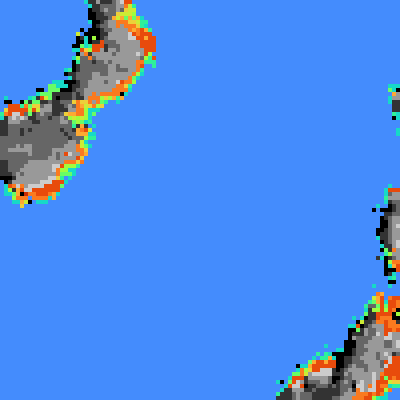
\includegraphics[width=0.32\linewidth]{img/experimentacion/naturales/Flame3/comparacion/flame_plot_2/paso30s_dispersa41_3x64_90s.png}\hfill
			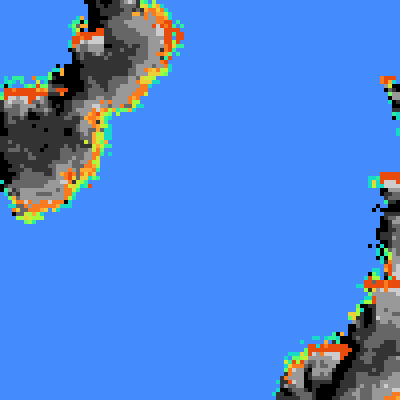
\includegraphics[width=0.32\linewidth]{img/experimentacion/naturales/Flame3/comparacion/flame_plot_2/paso30s_dispersa41_3x64_150s.png}\hfill
			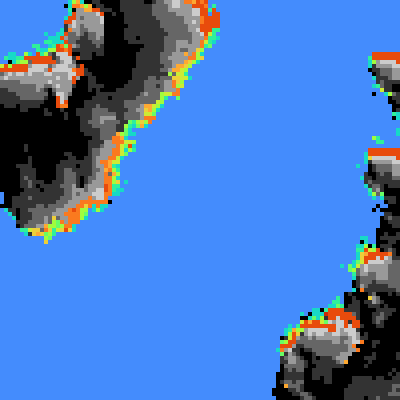
\includegraphics[width=0.32\linewidth]{img/experimentacion/naturales/Flame3/comparacion/flame_plot_2/paso30s_dispersa41_3x64_240s.png}
			\caption{30 s, dispersa, 3:64}
			\label{fig:flame_comparacion2_paso30s_dispersa41_3x64}
		\end{subfigure}
		\\[6pt]
		\begin{subfigure}[t]{0.48\textwidth}
			\centering
			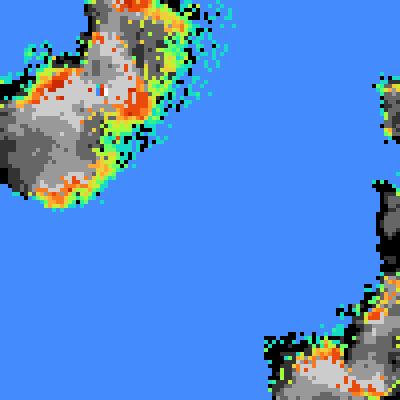
\includegraphics[width=0.32\linewidth]{img/experimentacion/naturales/Flame3/comparacion/flame_plot_2/paso5s_9x9_4x256_90s.png}\hfill
			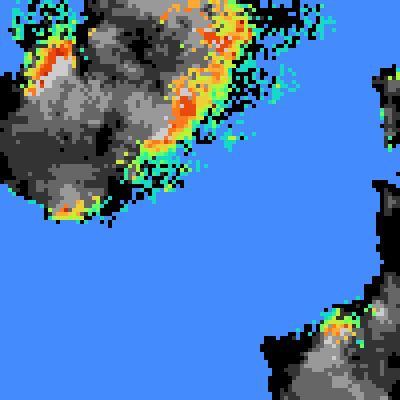
\includegraphics[width=0.32\linewidth]{img/experimentacion/naturales/Flame3/comparacion/flame_plot_2/paso5s_9x9_4x256_150s.png}\hfill
			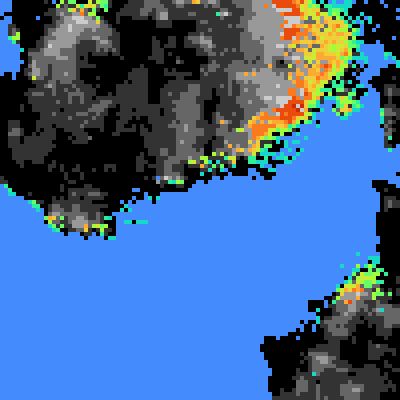
\includegraphics[width=0.32\linewidth]{img/experimentacion/naturales/Flame3/comparacion/flame_plot_2/paso5s_9x9_4x256_240s.png}
			\caption{5 s, $9 \times 9$, 4:256}
			\label{fig:flame_comparacion2_paso5s_9x9_4x256}
		\end{subfigure}
		\hfill
		\begin{subfigure}[t]{0.48\textwidth}
			\centering
			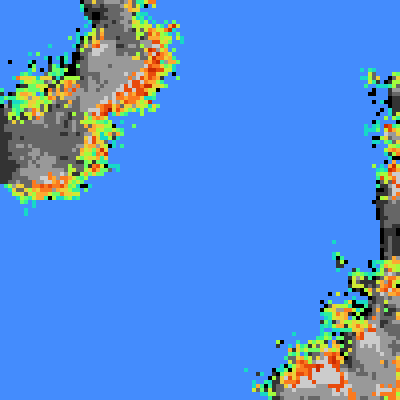
\includegraphics[width=0.32\linewidth]{img/experimentacion/naturales/Flame3/comparacion/flame_plot_2/paso15s_9x9_4x256_90s.png}\hfill
			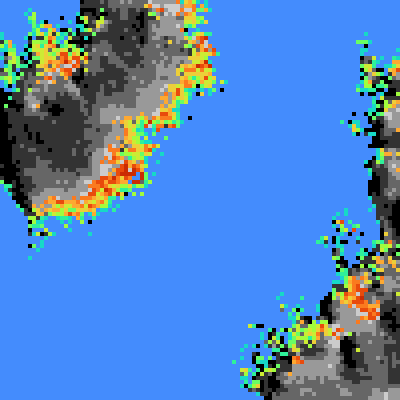
\includegraphics[width=0.32\linewidth]{img/experimentacion/naturales/Flame3/comparacion/flame_plot_2/paso15s_9x9_4x256_150s.png}\hfill
			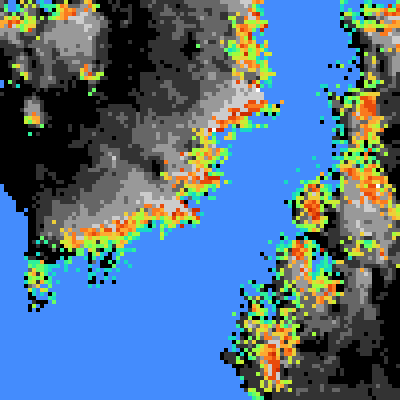
\includegraphics[width=0.32\linewidth]{img/experimentacion/naturales/Flame3/comparacion/flame_plot_2/paso15s_9x9_4x256_240s.png}
			\caption{15 s, $9 \times 9$, 4:256}
			\label{fig:flame_comparacion2_paso15s_9x9_4x256}
		\end{subfigure}
		\leyendaflame
		\caption{Evolución de flame\_plot\_2 (a) y simulación libre de las 9 configuraciones de ambas pruebas, entrenadas con flame\_plot\_1. En cada una: 90, 150 y 240 s después de la imagen inicial.}
		\label{fig:flame_comparacion2}
	\end{figure}
		
	Este experimento está limitado por varias razones. La primera es la cantidad de información recopilada, ya que FLAME~3 es uno de los pocos conjuntos de datos que registran la propagación del fuego, y específicamente con vista cenital. Además, este experimento no contempla todas las variables del sistema: únicamente se utilizan células en un plano bidimensional, sin considerar otras variables como la altura, las carreteras, los árboles, la dirección del viento o la humedad, que cambian drásticamente la dinámica.

	La reducción del conjunto de datos a únicamente dos muestras no permite generalizar a múltiples escenarios, y aparecen comportamientos diferentes que dependen de la geografía del sistema. Por ejemplo, en flame\_plot\_1 los cambios de temperatura casi siempre ocurren cerca de la línea del fuego, es decir, el sistema se mantiene frío excepto cuando el fuego se aproxima. Por otro lado, en flame\_plot\_2 primero se propagan las temperaturas medias y después son alcanzadas por el fuego.

	Otra consideración fue la dirección de la propagación. Aunque se probó rotar el sistema, las rotaciones añaden ruido, ya que la cámara está orientada hacia el norte y, en ambas pruebas, el viento apunta al este, por lo que las llamas, o las temperaturas, se mueven en esa dirección.

	A diferencia de lo que ocurrió con los sistemas ya conocidos, la red neuronal no tuvo el mismo éxito al intentar replicar el comportamiento. Sin embargo, algunas de las configuraciones sí pueden utilizarse para mostrarlo. En este caso, la selección visual de los experimentos tuvo como objetivo recoger aquellas configuraciones que podrían simular la propagación del fuego y la colisión de diferentes frentes, con una velocidad constante, sin generación espontánea de fuego y sin que un mismo lugar se queme dos veces.

	De este experimento podemos concluir que podría ser posible replicar estos sistemas con la cantidad de información suficiente para generalizarlos a cualquier entorno. Se pudieron diseñar autómatas celulares neuronales que propagan el fuego, pero basados únicamente en el registro de temperaturas y no en la geografía, que aportaría información específica para ayudar al sistema.
	



	\subsection{Simulación de tormentas}

El segundo sistema natural es el movimiento de las tormentas. A diferencia del fuego, que solo avanza sobre el terreno que no se ha quemado, una tormenta se desplaza con el viento, crece, se debilita y puede aparecer en zonas donde antes no llovía.

Este experimento se alimenta del conjunto de datos SEVIR (\textit{Storm EVent ImagRy}) \cite{veillette2020sevir}, que reúne más de 10,000 eventos meteorológicos registrados en los Estados Unidos entre 2017 y 2019. Cada evento cubre una zona de $384 \times 384$ km durante 4 horas y contiene imágenes de radar y de satélite. De todas ellas, solo se utiliza el VIL (\textit{vertically integrated liquid}), que mide la cantidad de agua líquida en la columna de aire sobre cada kilómetro cuadrado: un valor alto indica lluvia intensa o granizo. Cada evento tiene 49 imágenes de $384 \times 384$ píxeles (1 km por píxel), una cada 5 minutos.

Del conjunto completo se descargaron los 19,093 eventos que tienen VIL completo: 3,536 corresponden a tormentas registradas en la base de datos de eventos severos y 15,557 a eventos aleatorios. En este experimento solo se utilizan las tormentas.

\subsubsection{Preprocesamiento de los datos}

Para la limpieza del conjunto de datos, se procedió de la siguiente manera:

\begin{enumerate}
	\item Escalado de la evolución: Cada imagen se reduce de $384 \times 384$ a $96 \times 96$ células promediando bloques de $4 \times 4$ píxeles, por lo que cada célula representa 4 km. Con esta escala, una tormenta avanza alrededor de una célula por paso, lo que permite capturar su movimiento con una vecindad pequeña.

	\item Discretización: Se utilizan los 6 umbrales de VIL que proponen los autores de SEVIR para evaluar pronósticos (16, 74, 133, 160, 181 y 219, en la escala de 0 a 255 del conjunto de datos), lo que da 7 estados: el estado 0 indica que no hay lluvia y el estado 6, la lluvia más intensa (tabla \ref{tab:sevir_estados}). En adelante, se considera que una célula tiene tormenta si su estado es 2 o mayor, es decir, si su VIL es de al menos 74. La figura \ref{fig:sevir_preprocesamiento} muestra el resultado de ambos pasos.

	\item Selección de eventos: Para que la red no aprenda que las tormentas aparecen de la nada, se eligen al azar eventos en los que al menos el 2\% de las células tienen tormenta desde la primera imagen. El conjunto de entrenamiento tiene 40 tormentas de 2018 y el de prueba, 20 tormentas de 2019, por lo que la red se prueba con tormentas de otro año que nunca vio.
\end{enumerate}

\begin{table}[htbp]
	\centering
	\footnotesize
	\begin{tabular}{cccc}
		\toprule
		& & \textbf{Porcentaje en} & \textbf{Porcentaje en} \\
		\textbf{Estado} & \textbf{VIL} & \textbf{entrenamiento} & \textbf{prueba} \\ \midrule
		0 & 0--16 & 70.76 & 68.01 \\
		1 & 16--74 & 12.63 & 15.19 \\
		2 & 74--133 & 11.33 & 12.41 \\
		3 & 133--160 & 3.15 & 2.52 \\
		4 & 160--181 & 1.09 & 0.90 \\
		5 & 181--219 & 0.87 & 0.75 \\
		6 & 219--255 & 0.17 & 0.21 \\
		\bottomrule
	\end{tabular}
	\caption{Estados de SEVIR según el VIL de cada célula y su porcentaje en los conjuntos de entrenamiento (40 tormentas de 2018) y prueba (20 tormentas de 2019).}
	\label{tab:sevir_estados}
\end{table}

\definecolor{sevir0}{HTML}{F2F2F2}\definecolor{sevir1}{HTML}{9BE39B}\definecolor{sevir2}{HTML}{2E9E3A}
\definecolor{sevir3}{HTML}{F5D90A}\definecolor{sevir4}{HTML}{F28C1E}\definecolor{sevir5}{HTML}{D7191C}
\definecolor{sevir6}{HTML}{B10DC9}
\newcommand{\estadosevir}[2][black]{\fcolorbox{gray}{sevir#2}{\makebox[1.1em]{\textcolor{#1}{#2}}}}
\newcommand{\leyendasevir}{%
	\par\medskip
	{\footnotesize\setlength{\fboxsep}{1pt}%
	Estado: \estadosevir{0}\estadosevir{1}\estadosevir[white]{2}\estadosevir{3}\estadosevir{4}%
	\estadosevir[white]{5}\estadosevir[white]{6}\par}}

\begin{figure}[htbp]
	\centering
	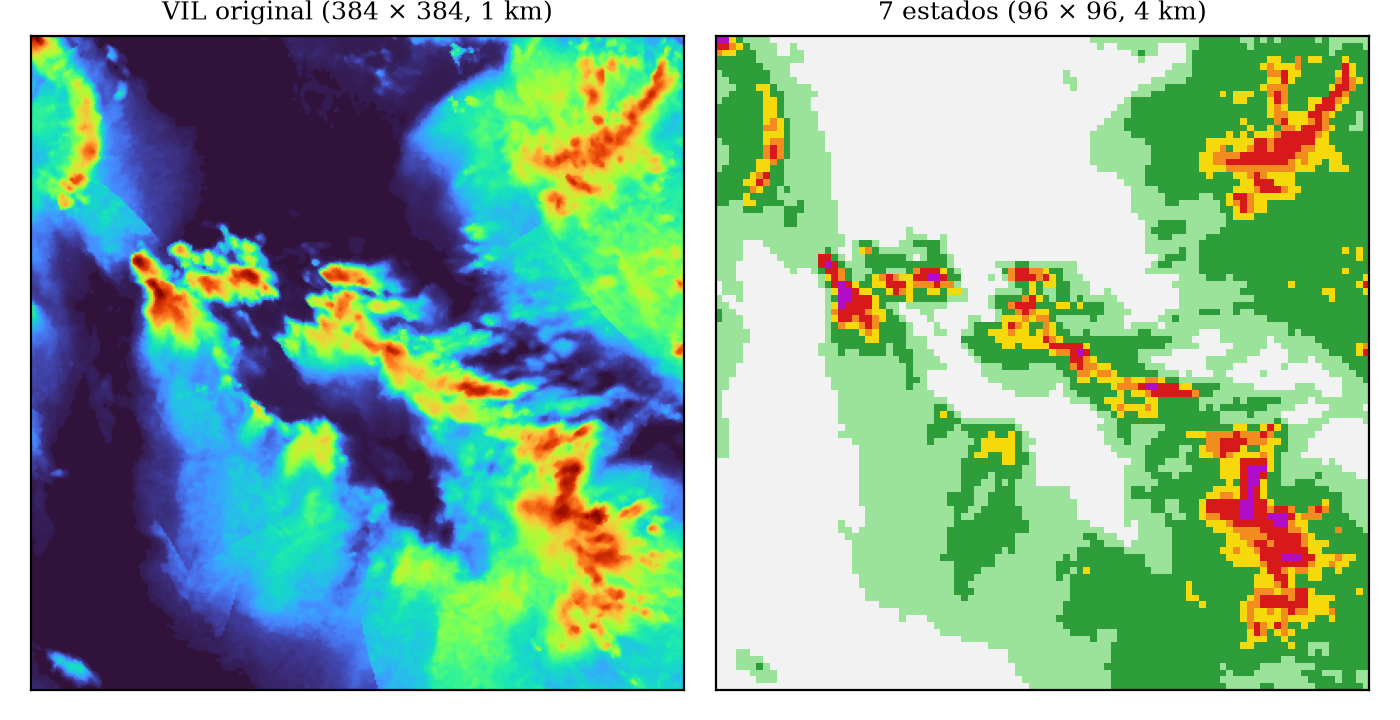
\includegraphics[width=0.8\linewidth]{img/experimentacion/naturales/SEVIR/preprocesamiento.png}
	\leyendasevir
	\caption{Primera imagen de una tormenta del conjunto de prueba (27 de mayo de 2019): VIL original y sus 7 estados después del escalado.}
	\label{fig:sevir_preprocesamiento}
\end{figure}

\subsubsection{Capacidad de replicación}

Se probaron 4 configuraciones: vecindad de $5 \times 5$ (25 vecinos) o de $9 \times 9$ (81 vecinos), y capas ocultas de 2:32:ReLU o 3:64:ReLU, con capa de salida 7:Linear. Todas usan \textit{one-hot}, por lo que la capa de entrada tiene $25 \times 7 = 175$ entradas con la vecindad de $5 \times 5$ y $81 \times 7 = 567$ con la de $9 \times 9$. Todas se entrenaron durante 30 épocas con entropía cruzada como función de pérdida, una tasa de aprendizaje inicial de 0.001 con reducción exponencial hasta 0.00001, un tamaño del lote de 8,192, frontera abierta y semilla aleatoria 42. El conjunto de entrenamiento tiene 17,694,720 muestras (40 tormentas, 48 pasos y $96 \times 96$ células); a diferencia de FLAME~3, cada entrenamiento tardó menos de un minuto.

Al igual que en FLAME~3, las redes se comparan con la predicción sin cambio, que supone que la siguiente imagen es igual a la actual. Se usan dos medidas:

\begin{enumerate}
	\item La exactitud es el porcentaje de células con el estado correcto.
	\item El área con tormenta indica qué tanto se parecen las células con tormenta (estado 2 o mayor) de la simulación a las reales. Un valor de 100\% significa que son idénticas.
\end{enumerate}

Ambas medidas se calculan de dos formas: prediciendo un solo paso desde cada imagen real de las 20 tormentas de prueba, y en la simulación libre, en la que la red parte de la primera imagen y evoluciona sola con sus propias predicciones durante 4 horas.

La tabla \ref{tab:sevir_resultados} muestra los resultados. Las 4 configuraciones superan a la predicción sin cambio en todas las medidas, aunque por poco: en un paso aciertan entre el 89.30 y el 89.37\% de las células, contra el 87.64\% de la predicción sin cambio, y en la simulación libre su área con tormenta se parece a la real entre un 4 y un 5\% más que la de la predicción sin cambio a los 30, 60 y 120 minutos. Las diferencias entre configuraciones son muy pequeñas: aumentar la vecindad o el tamaño de la red reduce la pérdida, pero no mejora la simulación libre.

\begin{table}[htbp]
	\centering
	\footnotesize
	\setlength{\tabcolsep}{4pt}
	\begin{tabular}{@{}cccccccc@{}}
		\toprule
		& & & & & \multicolumn{3}{c}{\textbf{Área con tormenta en}} \\
		& & & \multicolumn{2}{c}{\textbf{Un paso}} & \multicolumn{3}{c}{\textbf{la simulación libre}} \\
		\cmidrule(lr){4-5} \cmidrule(l){6-8}
		& & & & \textbf{Área con} & & & \\
		\textbf{Vecindad} & \textbf{Capas} & \textbf{Pérdida} & \textbf{Exactitud} & \textbf{tormenta} & \textbf{30 min} & \textbf{60 min} & \textbf{120 min} \\ \midrule
		\multicolumn{3}{c}{Predicción sin cambio} & 87.64\% & 76.93\% & 45.52\% & 32.43\% & 19.93\% \\ \midrule
		\multirow{2}{*}{$5 \times 5$} & 2:32 & 0.2266 & 89.30\% & 79.83\% & 50.24\% & 37.00\% & 23.77\% \\
		& 3:64 & 0.2245 & 89.31\% & 79.90\% & 50.22\% & 36.86\% & 23.38\% \\
		\multirow{2}{*}{$9 \times 9$} & 2:32 & 0.2226 & 89.35\% & 79.91\% & 50.02\% & 36.79\% & 23.55\% \\
		& 3:64 & 0.2192 & 89.37\% & 80.03\% & 49.94\% & 36.88\% & 23.28\% \\
		\bottomrule
	\end{tabular}
	\caption{Resultados en las 20 tormentas de prueba (2019) de las redes entrenadas con 40 tormentas de 2018.}
	\label{tab:sevir_resultados}
\end{table}

Sin embargo, la figura \ref{fig:sevir_comparacion} muestra que la simulación libre no se parece a una tormenta real. Las redes sí desplazan las tormentas, pero en pocos pasos las suavizan: las zonas de lluvia pierden sus detalles y se convierten en manchas uniformes, y las células más intensas se unen en bloques que dejan de moverse. Además, las redes nunca crean tormentas nuevas, mientras que en la evolución real aparecen nuevas líneas de tormenta y entran otras desde fuera del espacio.

\begin{figure}[htbp]
	\centering
	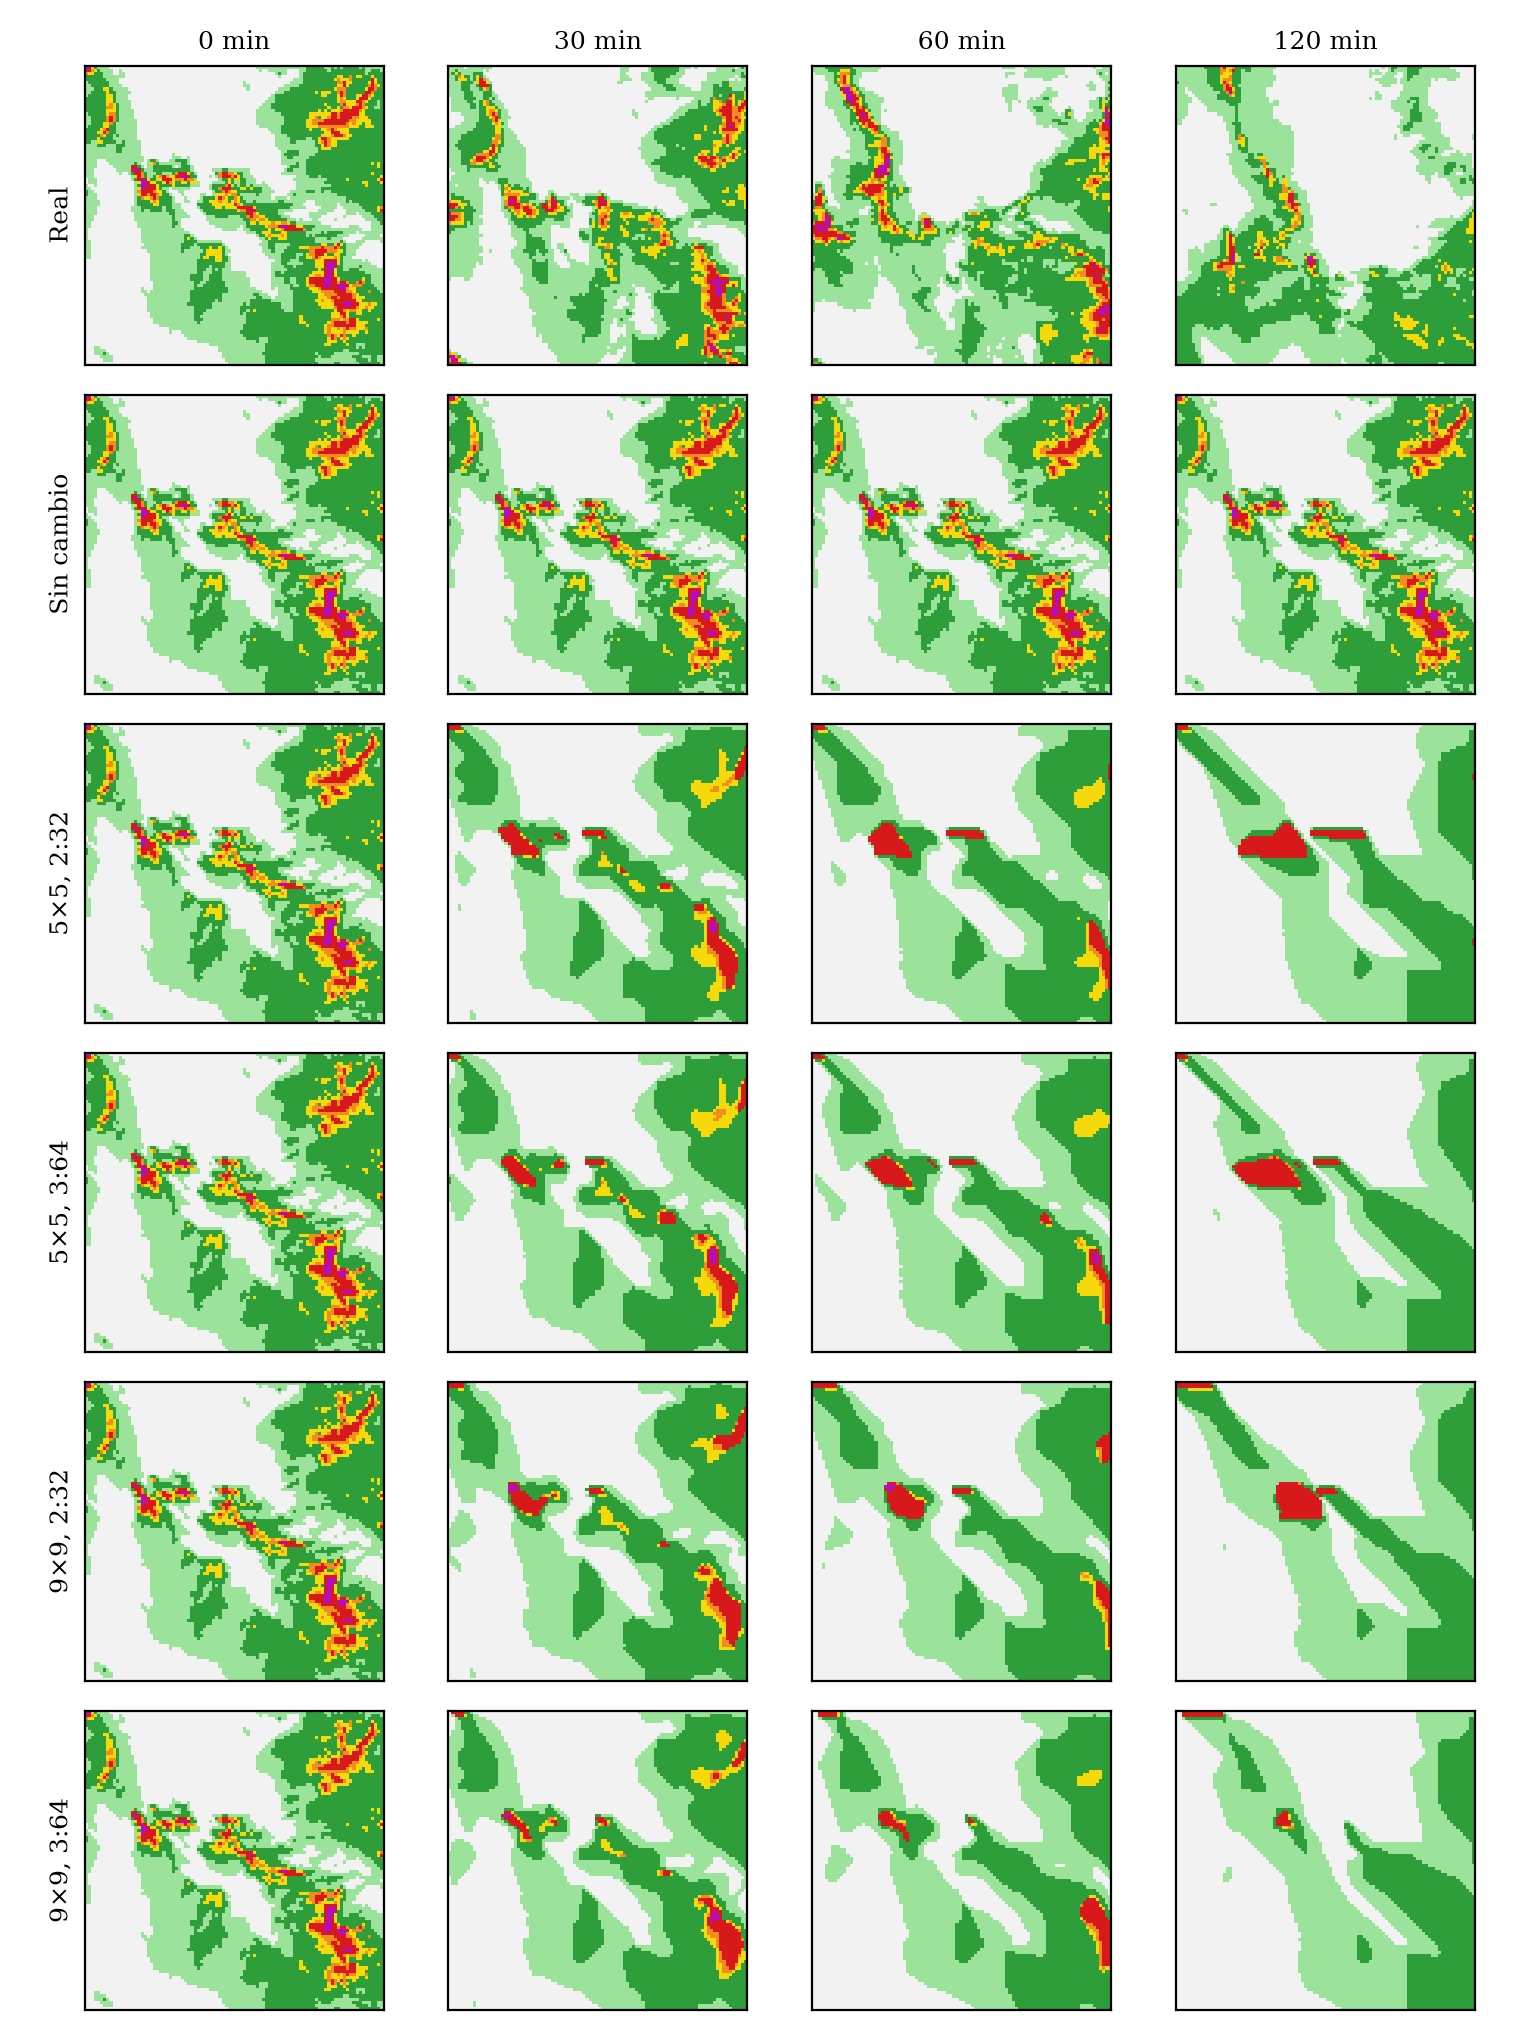
\includegraphics[width=0.8\linewidth]{img/experimentacion/naturales/SEVIR/comparacion.png}
	\leyendasevir
	\caption{Evolución real de la tormenta de la figura \ref{fig:sevir_preprocesamiento}, predicción sin cambio y simulación libre de las 4 configuraciones a los 0, 30, 60 y 120 minutos.}
	\label{fig:sevir_comparacion}
\end{figure}

Esto también se observa en la figura \ref{fig:sevir_area}: en las tormentas de prueba, el área con tormenta real crece del 12.3 al 19.7\% del espacio durante las 4 horas, mientras que en la simulación libre de todas las redes se reduce hasta un 9 o 10\%. Es decir, las redes aprendieron a mover y a debilitar las tormentas, pero no a formarlas ni a intensificarlas.

\begin{figure}[htbp]
	\centering
	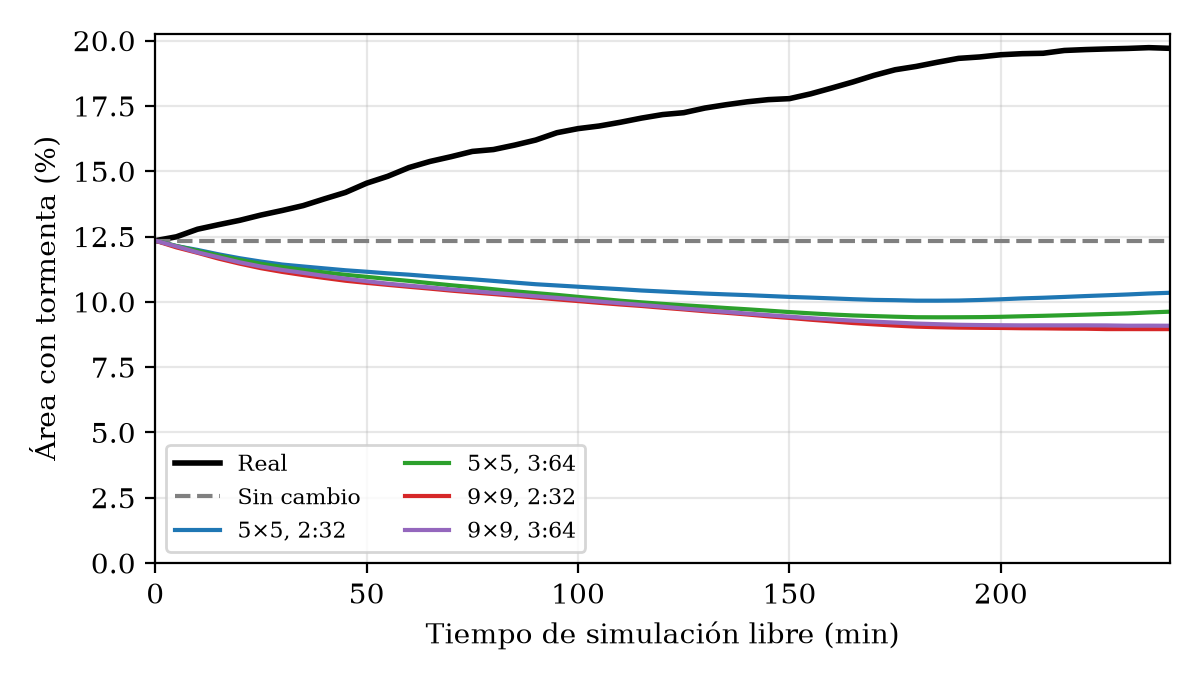
\includegraphics[width=0.75\linewidth]{img/experimentacion/naturales/SEVIR/area.png}
	\caption{Porcentaje del espacio con tormenta (estado 2 o mayor) durante la simulación libre, promedio de las 20 tormentas de prueba.}
	\label{fig:sevir_area}
\end{figure}

Este comportamiento tiene una explicación: cuando la red no puede saber si una célula va a llover más o menos, elige el estado más probable según los datos de entrenamiento, que casi siempre es uno de menos lluvia. Paso a paso, esta elección borra los detalles y debilita las tormentas. Al igual que en FLAME~3, la dinámica depende de variables que no están en las imágenes, como la temperatura, la humedad o el viento a distintas alturas, por lo que la vecindad no contiene toda la información necesaria para predecir el siguiente paso.

\subsubsection{Barrido de configuraciones}

Para saber si el resultado anterior se debe a la poca cantidad de datos o a la configuración de la red, se realizó un barrido con más tormentas, redes más grandes y más vecindades. Se utilizaron las 1,996 tormentas que cumplen la condición de selección para entrenar (1,286 de 2018 y 710 de 2017) y 200 tormentas de 2019 para la prueba, entre las que están las 20 del experimento anterior. Los 7 estados no cambian.

El programa de entrenamiento guarda en memoria la vecindad de cada célula de cada paso, por lo que 40 tormentas completas con la vecindad de $11 \times 11$ ya ocupan cerca de 9 GB. Para usar más tormentas sin rebasar ese límite, de cada tormenta se toman solo algunas transiciones, es decir, pares de imágenes consecutivas, elegidas al azar.

Todas las redes se entrenaron igual que en el experimento anterior (30 épocas, entropía cruzada, tasa de aprendizaje de 0.001 a 0.00001 con reducción exponencial, lote de 8,192 y semilla aleatoria 42) y con frontera abierta: fuera del espacio todas las células están en el estado 0. Una tormenta que entra desde el borde no está en la imagen anterior, por lo que con una frontera periódica la red aprendería que las tormentas aparecen de la nada.

Se probaron 8 vecindades (figura \ref{fig:sevir_vecindades}): 3 cuadradas, 3 circulares y 2 dispersas, la de FLAME~3 y una en forma de estrella, con un núcleo de $5 \times 5$ y 8 rayos que llegan hasta 11 células (44 km) de distancia. Todas tienen como máximo 128 vecinos, por lo que se pueden usar en el simulador. Las capas ocultas fueron 2:32:ReLU, 3:64:ReLU, 8:64:ReLU, 16:64:ReLU y 16:128:ReLU, con capa de salida 7:Linear, y la entrada fue lineal (el estado de cada vecino como un número) o con \textit{one-hot}.

\begin{figure}[htbp]
	\centering
	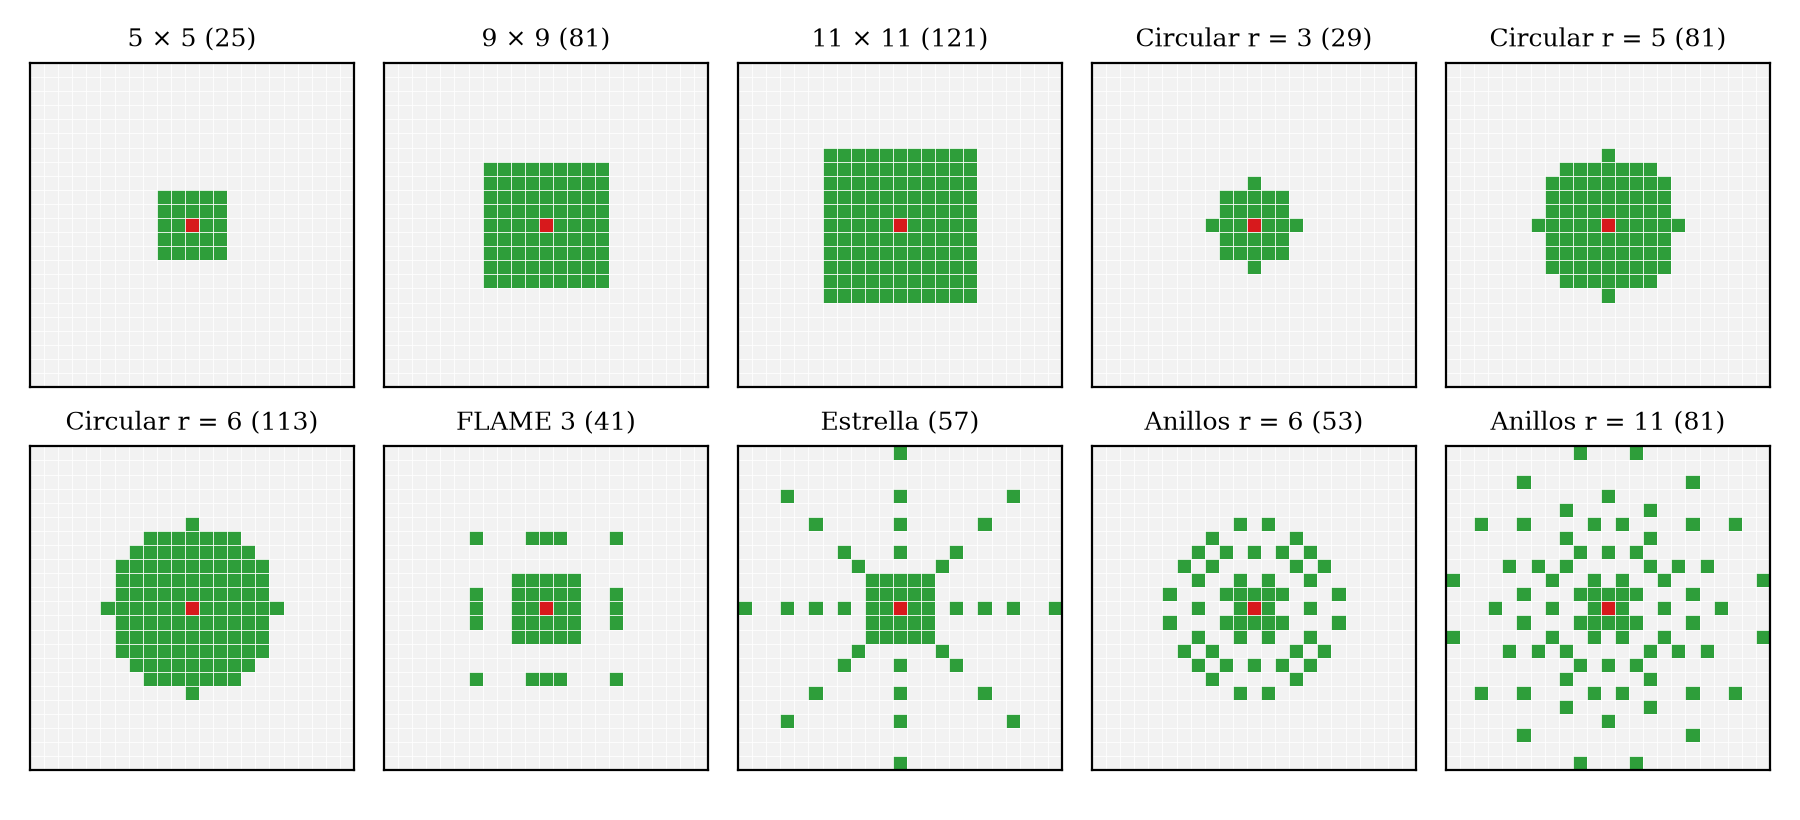
\includegraphics[width=\linewidth]{img/experimentacion/naturales/SEVIR/barrido_vecindades.png}
	\caption{Vecindades probadas en SEVIR y su número de vecinos. En rojo, la célula central. Las de anillos se probaron después del barrido.}
	\label{fig:sevir_vecindades}
\end{figure}

El barrido se dividió en tres fases:

\begin{enumerate}
	\item Pruebas pequeñas: las 80 combinaciones de vecindad, capas ocultas y entrada, con las mismas 40 tormentas completas del experimento anterior. Se eligieron las 4 mejores según el área con tormenta en un paso y en la simulación libre a los 60 y 120 minutos, y según qué tan parecida es la cantidad de tormenta simulada a la real a los 120 minutos.
	\item Más tormentas: las 4 mejores se entrenaron con 400 tormentas de 5 transiciones cada una (casi el mismo número de transiciones que con 40 tormentas completas, pero más variadas) y con 1,000 tormentas de 2 o 3 transiciones.
	\item Estabilidad: la mejor configuración se entrenó con las semillas aleatorias 1 y 2, con 100 épocas y con 4 estados en lugar de 7.
\end{enumerate}

La tabla \ref{tab:sevir_barrido_vecindad} muestra el promedio de las 10 redes de cada vecindad en la primera fase. Las 80 redes superan a la predicción sin cambio en todas las medidas, pero quedan muy cerca unas de otras: el área con tormenta en un paso va de 81.95 a 82.40\% y en la simulación libre a los 60 minutos, de 39.63 a 41.57\%. Las vecindades que llegan a 4 o más células de distancia ($9 \times 9$, $11 \times 11$, circulares de radio 5 y 6, y la de FLAME~3) son un poco mejores que las que llegan a 2 o 3 células. La vecindad de FLAME~3 da casi el mismo resultado que la de $11 \times 11$ con la tercera parte de los vecinos.

\begin{table}[htbp]
	\centering
	\footnotesize
	\setlength{\tabcolsep}{4pt}
	\resizebox{\linewidth}{!}{%
	\begin{tabular}{@{}cccccccc@{}}
		\toprule
		& & & \multicolumn{2}{c}{\textbf{Un paso}} & \multicolumn{2}{c}{\textbf{Área con tormenta en}} & \textbf{Tormenta simulada} \\
		\cmidrule(lr){4-5}
		& & & & \textbf{Área con} & \multicolumn{2}{c}{\textbf{la simulación libre}} & \textbf{respecto a la real} \\
		\cmidrule(lr){6-7}
		\textbf{Vecindad} & \textbf{Vecinos} & \textbf{Pérdida} & \textbf{Exactitud} & \textbf{tormenta} & \textbf{60 min} & \textbf{120 min} & \textbf{a los 120 min} \\ \midrule
		\multicolumn{3}{c}{Predicción sin cambio} & 87.79\% & 77.98\% & 31.78\% & 20.02\% & -- \\ \midrule
		$5 \times 5$ & 25 & 0.2261 & 90.13\% & 82.20\% & 40.02\% & 26.79\% & 65.25\% \\
		$9 \times 9$ & 81 & 0.2215 & 90.17\% & 82.28\% & 40.73\% & 27.95\% & 68.56\% \\
		$11 \times 11$ & 121 & 0.2199 & 90.16\% & 82.26\% & 40.94\% & 28.33\% & 70.22\% \\
		Circular, radio 3 & 29 & 0.2251 & 90.14\% & 82.22\% & 40.25\% & 27.08\% & 66.47\% \\
		Circular, radio 5 & 81 & 0.2214 & 90.17\% & 82.26\% & 40.89\% & 28.27\% & 70.91\% \\
		Circular, radio 6 & 113 & 0.2204 & 90.17\% & 82.28\% & 40.90\% & 28.06\% & 69.37\% \\
		FLAME~3 & 41 & 0.2221 & 90.17\% & 82.28\% & 40.85\% & 28.00\% & 67.99\% \\
		Estrella & 57 & 0.2196 & 90.15\% & 82.25\% & 40.57\% & 27.89\% & 64.99\% \\
		\bottomrule
	\end{tabular}}
	\caption{Primera fase del barrido: promedio de las 10 redes de cada vecindad (5 tamaños de capas ocultas, entrada lineal y \textit{one-hot}), entrenadas con 40 tormentas de 2018 y probadas en 200 tormentas de 2019.}
	\label{tab:sevir_barrido_vecindad}
\end{table}

El tamaño de la red tiene un efecto todavía menor (tabla \ref{tab:sevir_barrido_capas}): pasar de 2:32:ReLU a 16:128:ReLU reduce la pérdida, pero el área con tormenta a los 60 minutos solo sube de 40.34 a 40.83\%, mientras que el tiempo de entrenamiento crece de 35 a 89 segundos. La entrada lineal y el \textit{one-hot} dan prácticamente el mismo resultado (40.74 y 40.55\% a los 60 minutos), y las 4 mejores redes usan entrada lineal: circular de radio 5 con 16:128:ReLU, $11 \times 11$ con 16:64:ReLU, circular de radio 6 con 16:128:ReLU y $11 \times 11$ con 16:128:ReLU.

\begin{table}[htbp]
	\centering
	\footnotesize
	\begin{tabular}{@{}ccccccc@{}}
		\toprule
		& & & \multicolumn{2}{c}{\textbf{Un paso}} & \multicolumn{2}{c}{\textbf{Área con tormenta en}} \\
		\cmidrule(lr){4-5}
		& & \textbf{Tiempo} & & \textbf{Área con} & \multicolumn{2}{c}{\textbf{la simulación libre}} \\
		\cmidrule(l){6-7}
		\textbf{Capas} & \textbf{Pérdida} & \textbf{(s)} & \textbf{Exactitud} & \textbf{tormenta} & \textbf{60 min} & \textbf{120 min} \\ \midrule
		2:32 & 0.2275 & 34.7 & 90.11\% & 82.15\% & 40.34\% & 27.47\% \\
		3:64 & 0.2225 & 37.8 & 90.17\% & 82.24\% & 40.63\% & 27.84\% \\
		8:64 & 0.2210 & 54.5 & 90.18\% & 82.27\% & 40.65\% & 27.76\% \\
		16:64 & 0.2213 & 81.1 & 90.18\% & 82.33\% & 40.78\% & 27.95\% \\
		16:128 & 0.2179 & 88.9 & 90.15\% & 82.28\% & 40.83\% & 27.98\% \\
		\bottomrule
	\end{tabular}
	\caption{Primera fase del barrido: promedio de las 16 redes de cada tamaño de capas ocultas (8 vecindades, entrada lineal y \textit{one-hot}).}
	\label{tab:sevir_barrido_capas}
\end{table}

En la segunda fase (tabla \ref{tab:sevir_barrido_tormentas}), las 4 redes mejoran un poco al pasar de 40 tormentas completas a 400 tormentas con 5 transiciones cada una, aunque el número de transiciones es casi el mismo, es decir, la variedad de tormentas ayuda más que la cantidad de imágenes de cada una. En cambio, con 1,000 tormentas de solo 2 o 3 transiciones los resultados empeoran. La mejor configuración del barrido es la vecindad de $11 \times 11$ con 16:64:ReLU y entrada lineal, entrenada con 400 tormentas.

\begin{table}[htbp]
	\centering
	\footnotesize
	\setlength{\tabcolsep}{4pt}
	\begin{tabular}{@{}cccccccc@{}}
		\toprule
		& & & \textbf{Transiciones} & \textbf{Un paso} & \multicolumn{3}{c}{\textbf{Área con tormenta en}} \\
		& & & \textbf{por} & \textbf{Área con} & \multicolumn{3}{c}{\textbf{la simulación libre}} \\
		\cmidrule(l){6-8}
		\textbf{Vecindad} & \textbf{Capas} & \textbf{Tormentas} & \textbf{tormenta} & \textbf{tormenta} & \textbf{60 min} & \textbf{120 min} & \textbf{240 min} \\ \midrule
		\multicolumn{4}{c}{Predicción sin cambio} & 77.98\% & 31.78\% & 20.02\% & 10.78\% \\ \midrule
		\multirow{4}{*}{Circular, radio 5} & \multirow{4}{*}{16:128} & 40 & 48 & 82.34\% & 41.57\% & 29.20\% & 17.07\% \\
		& & 400 & 5 & 82.65\% & 41.67\% & 28.41\% & 15.66\% \\
		& & 400 & 7 & 82.59\% & 41.31\% & 28.04\% & 15.62\% \\
		& & 1,000 & 3 & 82.62\% & 41.52\% & 28.44\% & 15.82\% \\ \midrule
		\multirow{3}{*}{$11 \times 11$} & \multirow{3}{*}{16:64} & 40 & 48 & 82.36\% & 41.23\% & 28.43\% & 16.55\% \\
		& & 400 & 5 & \textbf{82.67\%} & \textbf{41.83\%} & \textbf{28.84\%} & 16.08\% \\
		& & 1,000 & 2 & 82.55\% & 40.49\% & 27.13\% & 14.17\% \\ \midrule
		\multirow{3}{*}{Circular, radio 6} & \multirow{3}{*}{16:128} & 40 & 48 & 82.40\% & 41.42\% & 28.44\% & 15.85\% \\
		& & 400 & 5 & 82.66\% & 41.68\% & 28.24\% & 15.15\% \\
		& & 1,000 & 2 & 82.56\% & 40.31\% & 26.82\% & 14.34\% \\ \midrule
		\multirow{3}{*}{$11 \times 11$} & \multirow{3}{*}{16:128} & 40 & 48 & 82.34\% & 41.38\% & 28.76\% & 16.88\% \\
		& & 400 & 5 & \textbf{82.67\%} & 41.68\% & 28.18\% & 15.51\% \\
		& & 1,000 & 2 & 82.57\% & 40.23\% & 26.82\% & 14.16\% \\
		\bottomrule
	\end{tabular}
	\caption{Segunda fase del barrido: las 4 mejores redes de la primera fase (entrada lineal) entrenadas con más tormentas. Con 48 transiciones se usa la tormenta completa. Con la vecindad circular de radio 5 caben 7 transiciones de 400 tormentas y 3 de 1,000; con las demás, solo 5 y 2.}
	\label{tab:sevir_barrido_tormentas}
\end{table}

En la tercera fase (tabla \ref{tab:sevir_barrido_estabilidad}), las semillas aleatorias 1 y 2 dan resultados casi iguales a los de la semilla 42, aunque el área con tormenta a los 60 minutos varía hasta 0.8\%, que es más que la diferencia entre muchas de las configuraciones de la primera fase. Entrenar 100 épocas reduce la pérdida, pero no mejora la simulación libre. Con 4 estados (sin lluvia, lluvia, tormenta y tormenta intensa) la red conserva un poco más de tormenta, aunque su exactitud no se puede comparar con la de 7 estados, porque con menos estados es más fácil acertar.

\begin{table}[htbp]
	\centering
	\footnotesize
	\setlength{\tabcolsep}{4pt}
	\begin{tabular}{@{}ccccccc@{}}
		\toprule
		& & \multicolumn{2}{c}{\textbf{Un paso}} & \multicolumn{2}{c}{\textbf{Área con tormenta en}} & \textbf{Tormenta simulada} \\
		\cmidrule(lr){3-4}
		& & & \textbf{Área con} & \multicolumn{2}{c}{\textbf{la simulación libre}} & \textbf{respecto a la real} \\
		\cmidrule(lr){5-6}
		\textbf{Prueba} & \textbf{Pérdida} & \textbf{Exactitud} & \textbf{tormenta} & \textbf{60 min} & \textbf{120 min} & \textbf{a los 120 min} \\ \midrule
		Semilla 42 & 0.2272 & 90.34\% & 82.67\% & 41.83\% & 28.84\% & 70.95\% \\
		Semilla 1 & 0.2277 & 90.35\% & 82.63\% & 41.19\% & 27.56\% & 66.49\% \\
		Semilla 2 & 0.2282 & 90.33\% & 82.63\% & 41.02\% & 27.41\% & 65.16\% \\
		100 épocas & 0.2250 & 90.36\% & 82.53\% & 40.70\% & 27.08\% & 62.45\% \\
		4 estados & 0.1798 & 92.36\% & 82.58\% & 42.24\% & 29.27\% & 76.76\% \\
		\bottomrule
	\end{tabular}
	\caption{Tercera fase del barrido: vecindad de $11 \times 11$, 16:64:ReLU, entrada lineal y 400 tormentas de 5 transiciones. Con 4 estados, la predicción sin cambio tiene una exactitud de 90.26\%; su área con tormenta es la misma que con 7 estados, porque la tormenta sigue siendo el VIL de al menos 74.}
	\label{tab:sevir_barrido_estabilidad}
\end{table}

\subsubsection{Vecindades de anillos}

Por último, se probaron dos vecindades dispersas circulares formadas por anillos (figura \ref{fig:sevir_vecindades}), con la configuración de la mejor red: la célula central, el anillo de radio 1 completo y anillos con 12 a 20 puntos repartidos a la misma distancia. La primera llega a 6 células de distancia con 53 vecinos y la segunda, a 11 células con 81 vecinos. Cada una se entrenó con las semillas aleatorias 42, 1 y 2.

La tabla \ref{tab:sevir_anillos} muestra que ambas dan prácticamente el mismo resultado que la vecindad de $11 \times 11$, con menos de la mitad de los vecinos en el caso de la de radio 6. Ver más lejos no mejora la simulación libre: la vecindad de radio 11 tiene el área con tormenta en un paso más alta y la menor variación entre semillas, pero conserva un poco menos de tormenta.

\begin{table}[htbp]
	\centering
	\footnotesize
	\setlength{\tabcolsep}{4pt}
	\begin{tabular}{@{}cccccccc@{}}
		\toprule
		& & \multicolumn{2}{c}{\textbf{Un paso}} & \multicolumn{3}{c}{\textbf{Área con tormenta en}} & \textbf{Tormenta simulada} \\
		\cmidrule(lr){3-4}
		& & & \textbf{Área con} & \multicolumn{3}{c}{\textbf{la simulación libre}} & \textbf{respecto a la real} \\
		\cmidrule(lr){5-7}
		\textbf{Vecindad} & \textbf{Vecinos} & \textbf{Exactitud} & \textbf{tormenta} & \textbf{60 min} & \textbf{120 min} & \textbf{240 min} & \textbf{a los 120 min} \\ \midrule
		\multicolumn{2}{c}{Predicción sin cambio} & 87.79\% & 77.98\% & 31.78\% & 20.02\% & 10.78\% & -- \\ \midrule
		$11 \times 11$ & 121 & 90.34\% & 82.64\% & 41.35\% & 27.93\% & 15.14\% & 67.53\% \\
		Anillos, radio 6 & 53 & 90.31\% & 82.59\% & 41.18\% & 27.61\% & 14.77\% & 65.99\% \\
		Anillos, radio 11 & 81 & 90.36\% & 82.68\% & 41.24\% & 27.69\% & 14.73\% & 64.49\% \\
		\bottomrule
	\end{tabular}
	\caption{Vecindades de anillos contra la de $11 \times 11$, con 16:64:ReLU, entrada lineal y 400 tormentas de 5 transiciones. Promedio de las semillas aleatorias 42, 1 y 2.}
	\label{tab:sevir_anillos}
\end{table}

Las figuras \ref{fig:sevir_barrido_comparacion} y \ref{fig:sevir_barrido_area} muestran que el comportamiento del experimento anterior no cambia con más tormentas ni con otras vecindades. Las redes conservan la forma general y la dirección de las tormentas, pero las convierten en manchas uniformes, y el área con tormenta de la simulación libre se queda entre el 11 y el 12\% del espacio, mientras que la real crece del 12.6 al 17.6\%.

\begin{figure}[htbp]
	\centering
	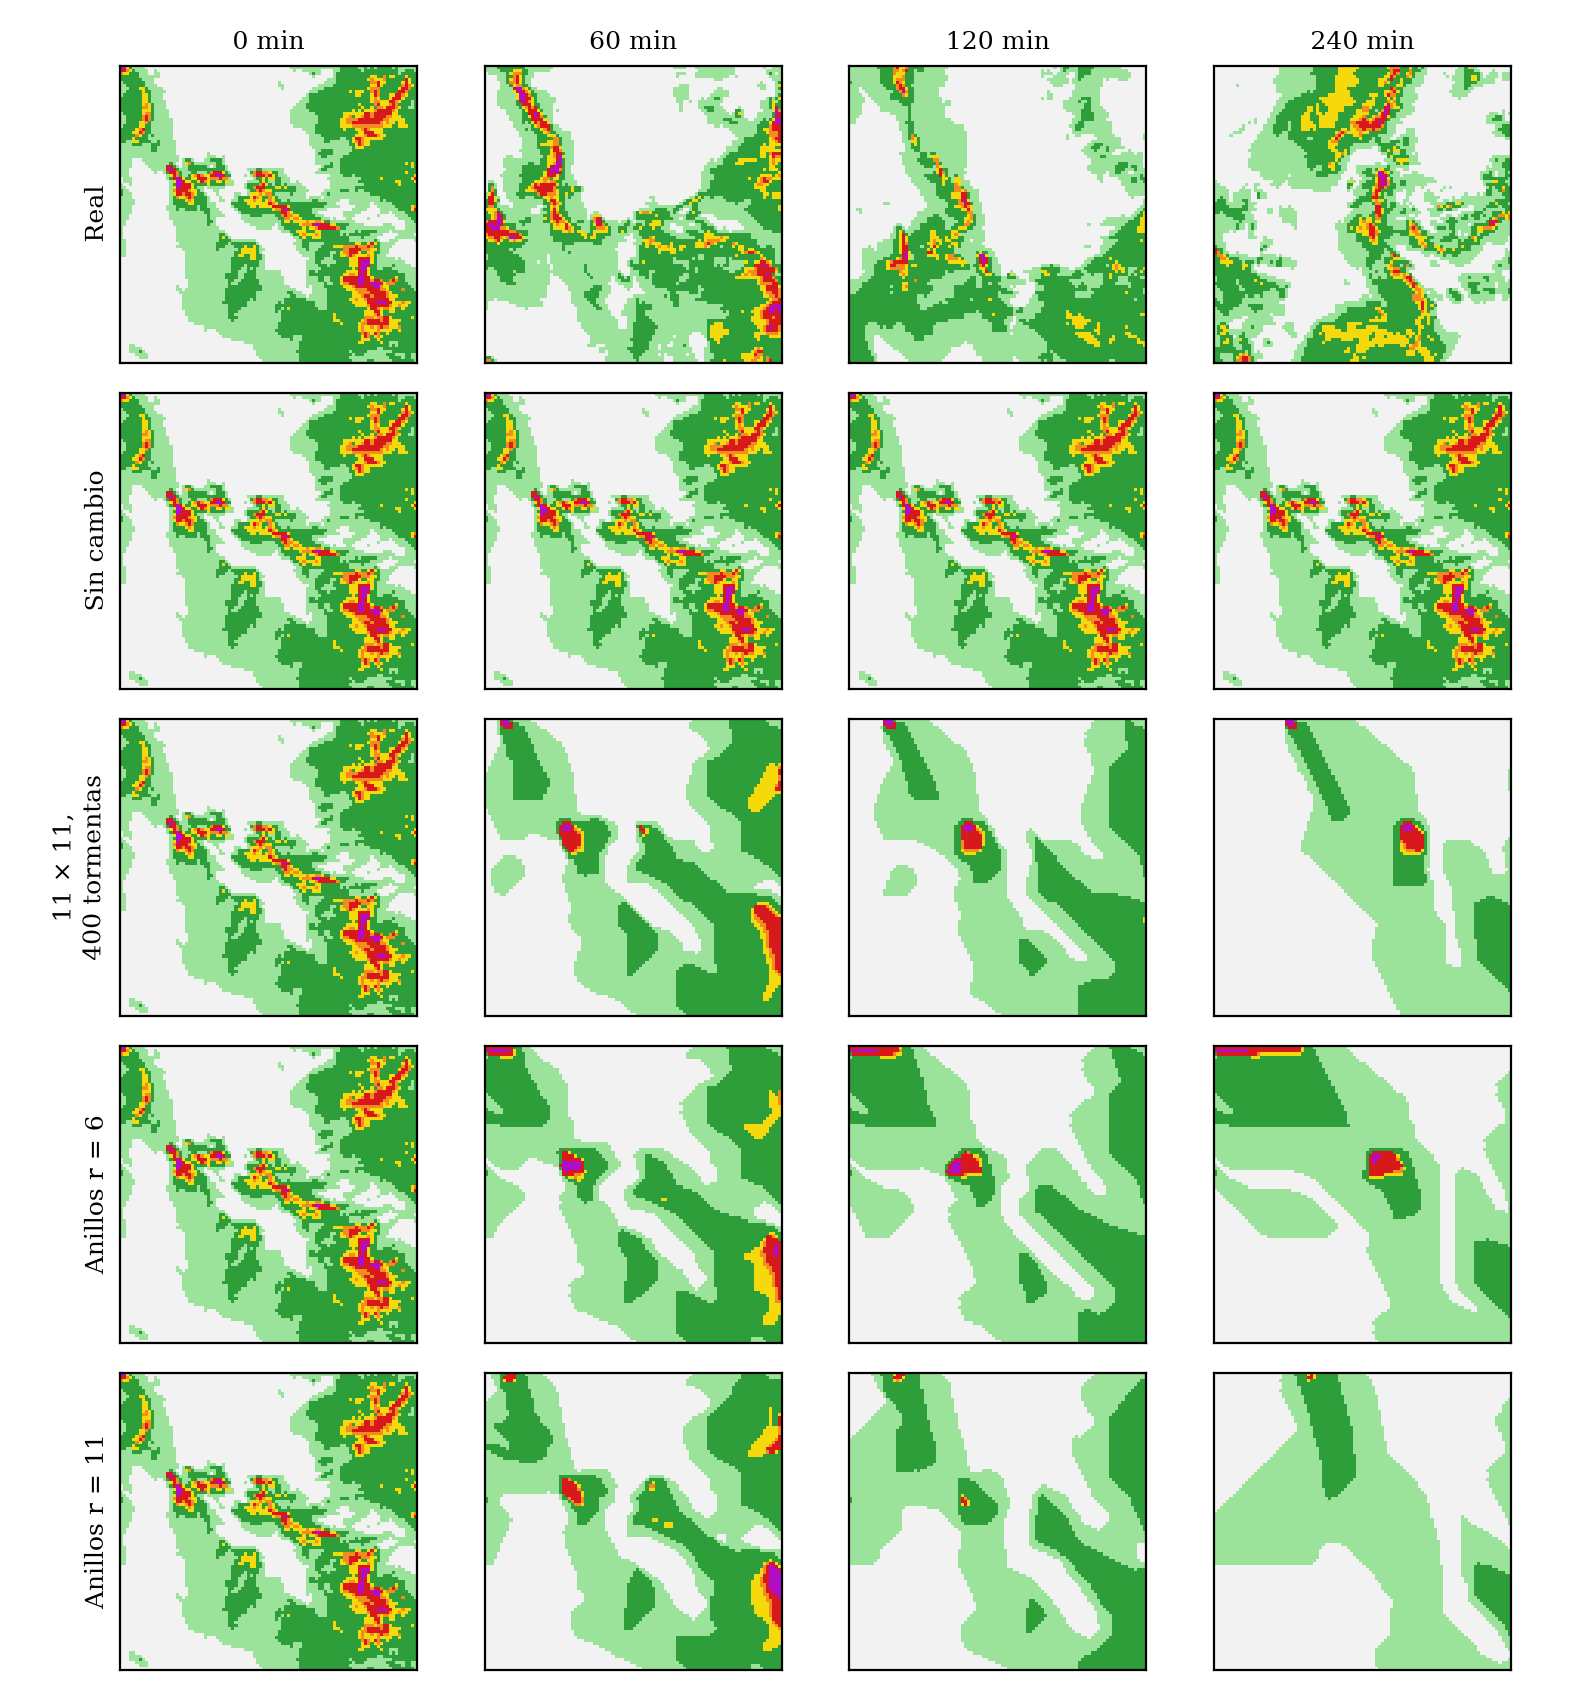
\includegraphics[width=0.8\linewidth]{img/experimentacion/naturales/SEVIR/barrido_comparacion.png}
	\leyendasevir
	\caption{Evolución real de la tormenta de la figura \ref{fig:sevir_preprocesamiento}, predicción sin cambio y simulación libre de la mejor red del barrido ($11 \times 11$) y de las vecindades de anillos, todas con 16:64:ReLU y 400 tormentas, a los 0, 60, 120 y 240 minutos.}
	\label{fig:sevir_barrido_comparacion}
\end{figure}

\begin{figure}[htbp]
	\centering
	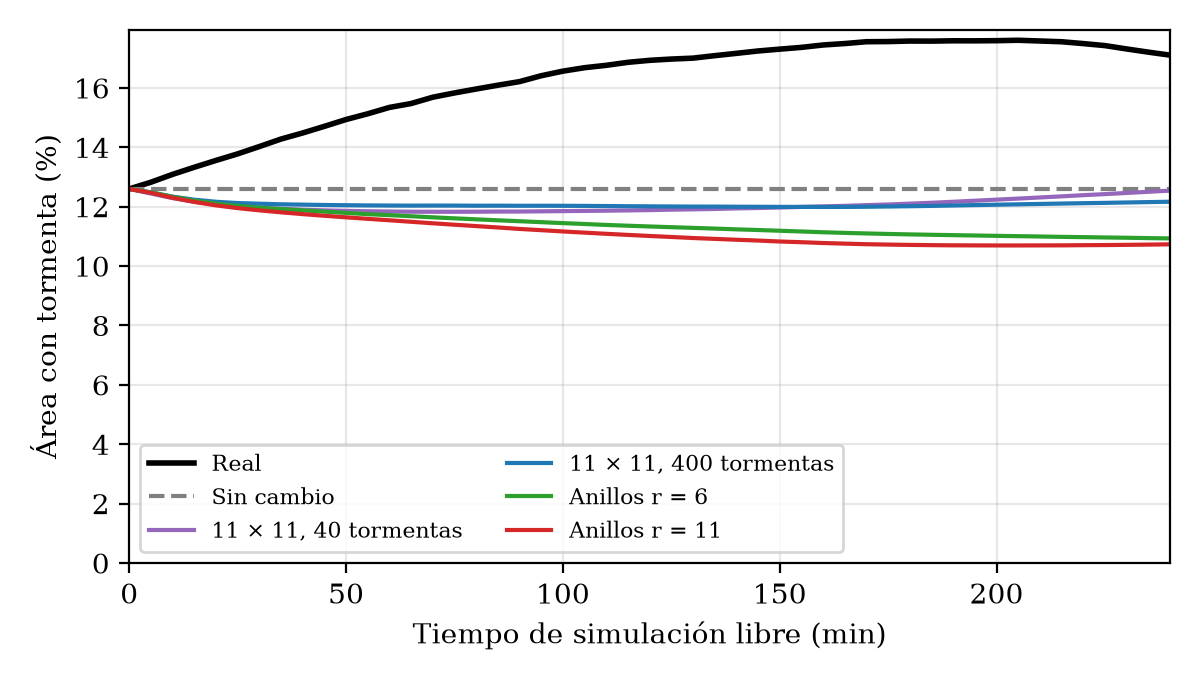
\includegraphics[width=0.75\linewidth]{img/experimentacion/naturales/SEVIR/barrido_area.png}
	\caption{Porcentaje del espacio con tormenta (estado 2 o mayor) durante la simulación libre, promedio de las 200 tormentas de prueba. Todas las redes usan 16:64:ReLU y entrada lineal.}
	\label{fig:sevir_barrido_area}
\end{figure}

\subsubsection{Desplazamiento de las tormentas}

Para saber qué aprendió la red, se midió cuánto se desplaza cada tormenta en 60 minutos, buscando el corrimiento de la primera imagen que mejor coincide con las células con tormenta a los 60 minutos. La tabla \ref{tab:sevir_desplazamiento} muestra que la red mueve casi todas las tormentas hacia el este, que es la dirección más común en los Estados Unidos, con mucha menos variación que las tormentas reales. La relación entre el desplazamiento de la red y el real es débil: la red se equivoca en promedio por unas 5 células, mientras que mover todas las tormentas con el desplazamiento promedio se equivoca por unas 6.

\begin{table}[htbp]
	\centering
	\footnotesize
	\begin{tabular}{@{}cccc@{}}
		\toprule
		& \textbf{Desplazamiento promedio} & \textbf{Variación entre tormentas} & \textbf{Relación con el real} \\
		& \textbf{hacia el este} & \textbf{(este--oeste / norte--sur)} & \textbf{(este--oeste / norte--sur)} \\ \midrule
		Real & 5.82 células (23 km) & 7.06 / 7.18 células & -- \\
		Red & 7.17 células (29 km) & 4.49 / 4.04 células & 0.36 / 0.51 \\
		\bottomrule
	\end{tabular}
	\caption{Desplazamiento de las células con tormenta en 60 minutos en las 200 tormentas de prueba, real y en la simulación libre de la mejor red ($11 \times 11$, 16:64:ReLU, 400 tormentas). La variación es la desviación estándar y la relación es la correlación entre el desplazamiento de la red y el real (1 sería idéntico).}
	\label{tab:sevir_desplazamiento}
\end{table}

Es decir, la red aprendió principalmente a desplazar las tormentas. La dirección en la que se mueve una tormenta depende del viento, que no está en las imágenes de VIL, y lo mismo ocurre con su crecimiento, que depende de la humedad y la temperatura del aire, y con las tormentas que entran desde fuera del espacio. Dos tormentas con la misma imagen pueden moverse en direcciones distintas, por lo que la vecindad no tiene la información necesaria para predecir el siguiente paso. Un autómata celular es un sistema cerrado, en el que la evolución depende solo de los estados de las células, y las tormentas no cumplen esa condición.

De este experimento podemos concluir que el autómata celular neuronal sí aprende parte de la dinámica de las tormentas a partir de su evolución, ya que supera a la predicción sin cambio en tormentas de un año que nunca vio. Sin embargo, con 7 estados y una sola variable, la simulación libre pierde las tormentas en pocas horas. El barrido muestra que este límite no depende de la cantidad de datos, del tamaño de la red ni de la vecindad, sino de que las tormentas son un sistema abierto, que depende de factores externos como el viento.

	\subsection{Crecimiento de moho mucilaginoso}

El ultimo experimento analiza el crecimiento de moho mucilaginoso, llamado \textit{Physarum polycephalum}, un moho que tiene características excepcionales al ser capaz de resolver laberintos, recordar rutas, adaptarse a obstáculos sin siquiera poseer cerebro o sistema nervioso. 

Este experimento utiliza el data
	
	
	\chapter{Líneas de investigación paralelas}

Durante el desarrollo de esta investigación se realizaron dos proyectos paralelos que contribuyeron al entendimiento de los sistemas complejos y, en particular, de los autómatas celulares neuronales. Ambos estudian el espacio de reglas de los autómatas celulares, es decir, el conjunto de todas las reglas locales posibles para un número dado de estados y de vecinos, desde dos perspectivas complementarias: cómo explorarlo para encontrar reglas con un comportamiento de interés y cómo medir qué tan parecidas son dos reglas por su comportamiento. Estas preguntas se relacionan directamente con los autómatas celulares neuronales, cuyas reglas no se diseñan a mano, sino que se obtienen mediante un proceso de optimización y, por lo tanto, también deben buscarse y compararse.

El primer proyecto, \textit{Adaptive Evolution in Totalistic Cellular Automaton}, se desarrolló en la \textit{Wolfram Summer School} 2025 y se presentó en la \textit{Wolfram Technology Conference} 2025. En él se buscan reglas de autómatas celulares totalísticos que, a partir de una sola celda activa, generen formas de vida finitas, combinando filtros que reducen el espacio de reglas con algoritmos de búsqueda de inspiración biológica. El segundo, \textit{Spectral Moments with Attractor Mass: A Similarity Index for One-Dimensional Cellular Automata}, se realizó en colaboración con Sukanta Das en la \textit{Indian Summer School on Cellular Automata} 2026 y propone un índice de similitud entre reglas basado en su grafo de transiciones, aplicable incluso a reglas con distinto número de estados o de vecinos. Ambos proyectos están relacionados: el primero agrupa reglas por su comportamiento a través de un grafo de mutaciones, mientras que el segundo busca cuantificar qué tan similares son dos reglas.

	\section{Adaptive Evolution in Totalistic Cellular Automaton}
\label{sec:evolucion-adaptativa}

En biología existen patrones de vida que crecen de forma indefinida y descontrolada, otros que mueren de inmediato bajo ciertas condiciones, y otros que persisten solo durante un número finito de pasos. Estos comportamientos también están presentes en reglas de autómatas celulares. En esta investigación \cite{angeles2025adaptive}, se estudiaron las reglas de autómatas celulares totalísticos unidimensionales capaces de generar formas de vida finitas \cite{hurtado2024finite}, es decir, reglas que, partiendo de una única célula activa, evolucionan un número de pasos antes de extinguirse. Posteriormente, el trabajo se amplió para su presentación en la \textit{Wolfram Technology Conference} 2025 \cite{angeles2025wtc}, con un filtro adicional y nuevas estrategias de búsqueda.

\subsection{Reducción del espacio de reglas}

Realizar una búsqueda exhaustiva de estas formas resulta computacionalmente inviable, ya que el número de reglas se incrementa de forma exponencial en función del número de estados y el tamaño de la vecindad. Para reducir el espacio de búsqueda, se aplican los siguientes cuatro filtros:

\begin{itemize}
	\item \textbf{Vida espontánea}: Se descartan las reglas que asignan un estado distinto de cero a la suma cero, pues generan actividad a partir de una vecindad completamente inactiva. La suma cero corresponde a la última posición del vector de la regla, de modo que solo se conservan las reglas cuyo número es múltiplo de $k$.
	
	\item \textbf{Muerte espontánea}: Si la penúltima posición vale 0, el patrón desaparece en el primer paso, por lo que esta posición debe ser distinta de cero.
	
	\item \textbf{Crecimiento infinito en triángulo}: Si la penúltima posición vale 1, las células de los extremos siempre ven una vecindad con suma 1 y reproducen el estado inicial, de modo que el patrón crece indefinidamente como un triángulo.
	
	\item \textbf{Crecimiento infinito completo}: El filtro anterior no elimina todos los triángulos infinitos. Un patrón crece como \textit{triángulo completo} si en el paso $t$ tiene un ancho de $2tr + 1$ células, y este crecimiento depende únicamente del \textit{vector intermedio}, formado por las posiciones $-k$ a $-2$ del vector de la regla, es decir, por las salidas de las sumas $k-1$ a $1$. Basta entonces probar cada vector intermedio con el resto de la regla en cero, y se conservan solo los que contienen a lo más un valor distinto de cero o no producen un triángulo completo. El resto del vector también influye en la evolución, pero con este filtro se evitan todos los triángulos completos.
\end{itemize}

Con los cuatro filtros basta estudiar alrededor del $8\%$ del total de reglas, y el número de reglas restantes puede aproximarse a partir del número $D_k$ de vectores intermedios aceptables. Aun con estos filtros, la búsqueda exhaustiva solo es viable en espacios pequeños, de hasta unos dos millones de reglas, como el de $k = 3$ y $r = 2.5$, con $3^{13} = 1{,}594{,}323$ reglas. 

\subsection{Estrategias de búsqueda}

Sobre el espacio filtrado se exploraron tres estrategias. En todas, la aptitud de una regla se define como el tiempo de vida de la forma que produce, es decir, el número de pasos hasta que el patrón desaparece:

\subsubsection{Búsqueda por fuerza bruta} 

Cada regla se trata como un nodo de un grafo. Sus vecinos son mutaciones de un solo dígito del vector de la regla. La búsqueda parte de la regla nula (regla 0), que puede convertirse en una forma de vida finita con una sola mutación, y explora su vecindad en anchura hasta alcanzar un número dado de nodos visitados. El resultado es un grafo de mutaciones. En él, todas las reglas que producen formas de vida finitas forman una componente conexa. Esto convierte la búsqueda en un problema de optimización: recorrer el grafo hacia las regiones con patrones más longevos.

\subsubsection{Algoritmo genético}

Para explorar espacios más grandes se aplicó un algoritmo genético, que mantiene una población de reglas candidatas y la hace evolucionar mediante selección, cruza, mutación y reemplazo. Se parte de una población aleatoria de $M$ reglas (por ejemplo, $M = 20$) y en cada generación se aplican cuatro pasos:
	
\begin{itemize}
	\item \textbf{Selección por torneo}: Se eligen al azar $n$ reglas de la población y la de mayor aptitud pasa a la población de padres hasta alcanzar el mismo tamaño que la población inicial.
	
	\item \textbf{Cruza uniforme}: Para cada par de padres se genera una máscara binaria. Si una posición vale 0, el primer hijo toma el gen del primer padre y el segundo hijo el del segundo; si vale 1, se intercambian. 
	
	\item \textbf{Mutación aleatoria}: Se eligen hijos al azar y se cambia el valor de una posición de su vector de regla.
	
	\item \textbf{Reemplazo elitista}: Se unen la población inicial y la de hijos, se ordenan por aptitud y se conservan las mejores $M$ reglas para la siguiente generación.
\end{itemize}
	
El proceso se repite hasta alcanzar la evolución más larga posible o un número dado de iteraciones. Se observó que las reglas más longevas comparten subconjuntos específicos de dígitos en su vector, que se comportan como motivos genéticos que mejoran la supervivencia, y que, generación tras generación, la población converge hacia regiones prometedoras del espacio de reglas. Sin embargo, el método es computacionalmente costoso, porque evalúa muchas reglas a la vez.
	
\subsubsection{Recocido simulado con distribución de Poisson}

El recocido simulado parte de una solución aleatoria y una temperatura alta. En cada paso propone una solución vecina y la acepta si es mejor. Si es peor, la acepta con una probabilidad que depende de la temperatura, la cual disminuye gradualmente hasta que el sistema se ``congela'' o se alcanza una condición de paro. Aceptar soluciones peores permite escapar de máximos locales, aunque, una vez congelado el sistema, es difícil salir de ellos.
	
Sobre esta idea, y en la línea del modelo mínimo de evolución biológica propuesto por Wolfram \cite{wolfram2024evolution}, se diseñó un algoritmo de evolución adaptativa. La búsqueda parte de la regla nula (regla 0) y calcula su tiempo de vida. En cada iteración se generan todas las mutaciones puntuales de la regla actual y se evalúa el tiempo de vida de cada una. Las mutaciones inválidas o degeneradas se descartan. El siguiente paso se elige al azar entre estas mutaciones, ponderadas por una distribución de Poisson con parámetro $\lambda$: cuando $\lambda$ es bajo, todos los vecinos tienen una probabilidad similar, lo que promueve una exploración amplia. Cuando es alto, los vecinos con mayor tiempo de vida son más probables, lo que promueve un refinamiento local. El parámetro $\lambda$ aumenta en cada iteración, de forma análoga al enfriamiento del recocido simulado. Cada vez que se encuentra una regla con un tiempo de vida mayor que el máximo registrado, esta se guarda y $\lambda$ se reduce temporalmente para explorar con amplitud la vecindad de la nueva regla, y luego vuelve a aumentar gradualmente. La búsqueda termina cuando $\lambda$ supera 5. En la práctica, incrementos de $\lambda$ menores que 0.5 dieron mejores resultados.

\subsection{Resultados y conclusiones}

La forma de vida finita más larga encontrada por búsqueda exhaustiva dura 109,521 pasos y se obtuvo con $k = 3$, $r = 2.5$, estado inicial 2 y un espacio de 699 células. Con $k = 3$ y $r = 1$, la forma de vida más larga dura 88 pasos, y en el grafo de mutaciones aparecen regiones de reglas que producen la misma evolución. En general, las formas de vida cortas son producidas por muchas reglas y están ampliamente distribuidas en el espacio de reglas, mientras que las largas son producidas por pocas reglas y se encuentran aisladas. En el grafo de mutaciones, las reglas que producen formas de vida similares forman grupos densamente conectados, mientras que las formas más largas y complejas aparecen en la periferia, con pocas conexiones. Por esta razón, las caminatas aleatorias son una estrategia débil.

En las ejecuciones del recocido simulado con distribución de Poisson desde la regla nula y con $r = 1$, la búsqueda alcanzó formas de vida de 88 pasos con $k = 3$ y de $1{,}800$ pasos con $k = 5$. Aceptar temporalmente reglas peores resultó necesario para explorar el espacio. Aun así, con $k = 4$ la búsqueda se estanca en configuraciones específicas, y con $k = 5$ es difícil pasar de un pico a otro, porque no existe un camino directo de mejoras sucesivas. Algoritmos más simples, como el ascenso de colinas (\textit{hill climbing}), no funcionaron bien porque se estancan muy rápido.

En conjunto, esta metodología permitió descubrir formas de vida finitas y proporcionó un marco para estudiar la estructura del espacio de reglas, la robustez de las formas de vida y los caminos evolutivos entre configuraciones. Además, al agrupar reglas por su comportamiento, el grafo de mutaciones se relaciona con la pregunta que motivó el segundo proyecto: qué tan similares son dos reglas.

Este proyecto se realizó en la \textit{Wolfram Summer School} 2025, en Bentley University, Massachusetts, EUA, bajo la mentoría de Willem Nielsen y a partir de una propuesta de Stephen Wolfram. Los resultados se publicaron en \textit{Wolfram Community} \cite{angeles2025adaptive}, donde fueron seleccionados para la columna \textit{Staff Picks}, y posteriormente se presentaron en la \textit{Wolfram Technology Conference} 2025 \cite{angeles2025wtc}. Este trabajo contribuyó a la publicación \textit{What's Special about Life? Bulk Orchestration and the Rulial Ensemble in Biology and Beyond}, de Stephen Wolfram \cite{wolfram2025life}, en cuyos agradecimientos se reconoce la ayuda del autor como afiliado del \textit{Wolfram Institute}.

	\section{Spectral Moments with Attractor Mass: A Similarity Index for One-Dimensional Cellular Automata}

La regla B3/S23, que define el juego de la vida, es solo una de las $2^{18}$ reglas que comparten su estructura: dos estados, vecindad semitotalística de Moore y una transición que depende únicamente del estado de la célula y del número de vecinos vivos. Existe una familia de reglas llamada \textit{life-like} \cite{lifewiki_life} que presenta un comportamiento similar al de la regla \textit{Life} (B3/S23) con pequeñas diferencias. Sin embargo, ¿cómo se decide qué reglas son similares? Las clasificaciones existen, pero su respuesta es siempre binaria: dos reglas son o no iguales. Surge entonces una segunda pregunta: ¿qué tan similares son? Esta pregunta dio pie a la investigación realizada con Sukanta Das \cite{angeles2027spectral}, donde se definió el método de momentos espectrales con masa de atractor, que asigna un grado de similitud entre dos reglas dadas, incluso si tienen distinto número de estados o de vecinos. 

\subsection{Relaciones exactas entre reglas}

El primer paso fue identificar las relaciones exactas entre las reglas aplicando cuatro criterios de equivalencia. Para ello se define el \textit{dominio} de una regla como la terna formada por la dimensión, los estados y los vecinos. Decimos que dos reglas pertenecen al mismo dominio si comparten los tres elementos. 

Dos de los criterios, la permutación de estados y las reglas espejo, son bien conocidos en la literatura y fueron revisados por Martínez \cite{Martinez2013note}; con ellos, las 256 reglas de los autómatas celulares elementales se reducen a 88 clases. Los otros dos son propuestos y comparan reglas con distinto número de estados y con distinto número de vecinos, por lo que se denominan reducción de estados y reducción de vecinos, respectivamente. Con ellos es posible mapear relaciones entre distintos espacios de reglas. Si $(x_1, \dots, x_m)$ es el estado de la vecindad y $\mathcal{R}$ la regla local, los cuatro criterios son:

\begin{itemize}
	\item \textbf{Permutación de estados.} Existe una biyección $\pi$ sobre el conjunto de estados tal que
	\[
	\mathcal{R}_2(x_1, \dots, x_m) = \pi\bigl(\mathcal{R}_1(\pi^{-1}(x_1), \dots, \pi^{-1}(x_m))\bigr),
	\]
	es decir, reetiquetar los estados deja la estructura sin cambios. En el caso binario, la única permutación no trivial es $\pi(x) = 1 - x$.
	
	\item \textbf{Reglas espejo.} Si $M(x_1, \dots, x_m) = (x_m, \dots, x_1)$ es la reflexión de la vecindad, entonces $\mathcal{R}_2 = \mathcal{R}_1 \circ M$: reflejar la configuración inicial, evolucionarla con la primera regla y reflejar el resultado produce la evolución de la segunda.
	
	\item \textbf{Reducción de estados.} Si un estado $a$ nunca es producido por la regla y toda vecindad que lo contiene produce siempre el mismo estado $b$, entonces $a$ solo puede aparecer en la configuración inicial y desaparece en el primer paso. La evolución coincide con la de la regla restringida a los estados restantes. Inversamente, toda regla de $q$ estados puede extenderse a $q + 1$ estados añadiendo un estado que nunca se produce.
	
	\item \textbf{Reducción de vecinos.} Si existe un vecino cuyo estado no afecta la transición, este puede eliminarse de la vecindad. Si no se encuentra en uno de los extremos, la vecindad se reajusta para que sea contigua, bajo la hipótesis de que la distancia entre vecinos solo transforma el espacio de la evolución y no el comportamiento. Esta reducción es la responsable de agrupar comportamientos y reducir de 88 a 81 clases.
\end{itemize}

Al aplicar iterativamente estas cuatro relaciones se construye un grafo de relaciones entre reglas de distintos dominios, cuyas componentes conexas son las clases de equivalencia. Se reducen de 88 a 81 clases. Aunque esta clasificación sigue siendo binaria, sirve como referencia para validar los métodos siguientes.

\subsection{Comparación estructural del grafo de transiciones}

Estas relaciones dependen únicamente del vector de la regla. Como alternativa, se analizó el comportamiento evolutivo que tienen todas las configuraciones iniciales en un espacio con frontera periódica de $n$ células. Cada configuración representa un nodo que evoluciona y se dirige a otro, creando un grafo funcional. Cada componente conexa tiene exactamente un ciclo o atractor del cual cuelgan árboles transitorios. Ambos generan la \textit{cuenca de atracción}. Para cada configuración $x$ se definen su periodo $p(x)$, la longitud del ciclo que alcanza, y su altura $h(x)$, el número mínimo de pasos necesario para alcanzarlo ($h(x) = 0$ si $x$ es periódica). Además, como la función global conmuta con las traslaciones del anillo, se construye el \textit{grafo cociente por traslaciones}, en el que todas las rotaciones de una configuración forman un solo nodo.

Decimos entonces que dos reglas tienen el mismo comportamiento si sus grafos de transiciones son isomorfos, lo cual se verifica de forma eficiente comparando sus formas canónicas. En los autómatas celulares elementales, el grafo completo distingue hasta 85 de las 88 clases (con $n = 6$) y el grafo cociente también hasta 85 (con $n = 10$). Usando ambos sobre el mismo espacio se distinguen las 88 clases con solo 6 células. No obstante, esta comparación sigue siendo binaria, se limita a reglas del mismo dominio y su resultado depende del tamaño $n$ del espacio.

\subsection{Métodos espectrales}

Para obtener una medida gradual, cada regla se representa mediante un vector numérico (\textit{embedding}) derivado del grafo de transiciones, de modo que la distancia coseno entre vectores funcione como índice de similitud. Se exploraron tres representaciones:

\subsubsection{Eigenvalores}

Se utilizan los eigenvalores ordenados de la matriz de adyacencia del grafo de transiciones. Este método tiene dos limitaciones. Por un lado, es ciego a los transitorios: los árboles solo aportan eigenvalores nulos, por lo que el espectro depende únicamente de los atractores. Por ejemplo, las reglas 0 y 8 tienen un único atractor y, aunque lo alcanzan en a lo más 1 y 2 pasos respectivamente, sus espectros son idénticos. Por otro lado, el número de eigenvalores es igual al número de configuraciones, por lo que solo pueden compararse reglas con el mismo número de estados sobre el mismo espacio.
	
\subsubsection{Momentos espectrales}

Para eliminar la dependencia del dominio, en lugar del espectro completo se mide, para cada paso $k = 1, \dots, K$, la proporción de configuraciones que regresan a sí mismas tras $k$ pasos:
\begin{equation}
	m_k = \frac{| \{ x \in \mathcal{C} : F^k(x) = x \} |}{N},
\end{equation}
donde $\mathcal{C}$ es el conjunto de configuraciones y $F$ la función global. La longitud del vector depende solo de la ventana $K$, por lo que es posible comparar reglas con distinto número de estados, de vecinos o de células. Sin embargo, como $m_k$ depende solo de los eigenvalores, hereda la ceguera a los transitorios.

\subsubsection{Momentos espectrales con masa de atractor} 

Para distinguir reglas como la 0 y la 8 es necesario medir, además de los atractores, con qué fuerza atraen al resto de las configuraciones, es decir, cuántas configuraciones llegan a cada atractor y en cuántos pasos. Cada ciclo se sigue activando cada $p$ pasos, como en los momentos espectrales, pero en cada activación se suman también las configuraciones que ya lo han alcanzado. Utilizando la altura y el periodo de cada configuración, se define
\begin{equation}
	\tilde{m}_k = \frac{| \{ x \in \mathcal{C} : p(x) \mid k \mbox{ y } h(x) \le k - p(x) \} |}{N}, \qquad k = 1, \dots, K.
\end{equation}
Es decir, una configuración cuenta en el paso $k$ si su atractor se activa en ese paso y la configuración ya lo había alcanzado antes de la activación previa: los nodos del ciclo ($h = 0$) cuentan desde la primera activación ($k = p$), los nodos con $1 \le h \le p$ desde la segunda ($k = 2p$), y así sucesivamente. Como toda configuración periódica cumple la condición cuando $p \mid k$, el vector se descompone como $\tilde{m}_k = m_k + t_k$, donde $t_k$ es la proporción de configuraciones transitorias que cuentan en el paso $k$. Así, el nuevo vector extiende los momentos espectrales con la información de las cuencas y conserva una longitud $K$ independiente del dominio, con la limitación de que un ciclo con $p > K$ nunca se activa.
	
Por ejemplo, con 5 células ($N = 32$), la regla 0 envía toda configuración al cero en un paso ($h \le 1$), mientras que en la regla 8 cada bloque de unos deja un 1 aislado que desaparece en el siguiente paso ($h \le 2$). De las 32 configuraciones, solo 12 llegan al cero en a lo más un paso. Sus vectores, $\tilde{m}^{(0)} = \frac{1}{32}(1, 32, 32, \dots)$ y $\tilde{m}^{(8)} = \frac{1}{32}(1, 12, 32, \dots)$, ya no son iguales, aunque sus momentos espectrales sí lo son.

\subsection{Resultados}

La tabla \ref{tab:clases-metodos} resume el número máximo de clases que distingue cada método entre las 88 reglas representativas de los autómatas celulares elementales, para tamaños $n = 1, \dots, 29$. La forma canónica es el método que más clases distingue, pero los momentos espectrales con masa de atractor son el segundo mejor: con $K = 60$ y $n \ge 6$, el grafo completo distingue entre 79 y 83 clases. Combinando $n = 3$ y $n = 6$ alcanza 86 y, junto con el cociente sobre el mismo tamaño, 87. Solo permanecen juntos los pares $\{1, 19\}$, cuyas alturas exactas son distintas pero caen en el mismo intervalo de $p$ pasos, y $\{4, 12\}$, que coinciden en la distribución de altura y periodo y difieren solo en la forma de los árboles. Los eigenvalores y los momentos espectrales simples, en cambio, se detienen en 77 clases.

\begin{table}[htbp]
	\centering
	\caption{Número máximo de clases distinguidas entre las 88 reglas representativas de los autómatas celulares elementales. ``Un tamaño'': mejor $n$; ``Todos'': combina los 29 tamaños; ``Completo + cociente'': ambos grafos sobre el mismo tamaño.}
	\label{tab:clases-metodos}
	\small
	\setlength{\tabcolsep}{4pt}
	\begin{tabular}{lccccc}
		\hline
		& \multicolumn{2}{c}{Grafo completo} & \multicolumn{2}{c}{Cociente} & Completo \\
		Método & Un tamaño & Todos & Un tamaño & Todos & + cociente \\
		\hline
		Forma canónica        & 85 & 88 & 85 & 85 & 88 \\
		Eigenvalores          & 74 & 77 & 63 & 68 & 77 \\
		Momentos espectrales  & 74 & 77 & 63 & 68 & 77 \\
		Masa de atractor      & 83 & 86 & 80 & 81 & 87 \\
		\hline
	\end{tabular}
\end{table}

Para evaluar el método como índice de similitud se utilizó la distancia coseno
\begin{equation}
	d(u, v) = 1 - \frac{u \cdot v}{\| u \| \, \| v \|}
\end{equation}
con $K = 60$, de la que se obtuvieron tres resultados principales.

\begin{itemize}
	\item \textbf{Una regla en espacios de distinto tamaño}: Al comparar cada autómata celular elemental consigo mismo en tamaños $n \neq n'$ con $n, n' \in \{8, \dots, 29\}$, la mediana de la distancia es 0.098 en el grafo completo y 0.001 en el cociente, frente a 0.47 y 0.23 entre reglas distintas del mismo tamaño. Sin embargo, como muchas reglas tienen vecinos muy cercanos, una regla solo se identifica consigo misma en el 25\% de los casos en el grafo completo y en el 33\% en el cociente. La comparación entre tamaños distintos solo es confiable para reglas cuyos atractores no dependen de $n$, como la negación (51) y la identidad (204). Las reglas de desplazamiento nunca se identifican en el grafo completo, porque la longitud de sus ciclos depende de los divisores de $n$, y las reglas caóticas y aditivas casi nunca se identifican. Por ello, en general es preferible comparar sobre el mismo tamaño.
	
	\item \textbf{Agrupamiento de los autómatas celulares elementales}: Con $n = 12$ y $K = 60$, el mejor agrupamiento de las 88 reglas representativas se obtuvo con $k$-medoides y 4 grupos (silueta de 0.70). Los grupos quedan separados por el periodo dominante de sus atractores (tabla \ref{tab:clusters}): reglas que envían casi todas las configuraciones a puntos fijos; reglas cuyos atractores se desplazan, con ciclos de periodo $n$ o $2n$; reglas con atractores de periodo 2, como la negación y las reglas aditivas; y reglas con ciclos largos. Las reglas caóticas no forman un grupo propio: en algunas, la mayoría de las configuraciones alcanza ciclos con periodo mayor que $K$, que nunca se activan, y como la distancia coseno descarta la magnitud del vector, terminan en el grupo de punto fijo (por ejemplo, la regla 30). En otras, la mayoría de las configuraciones sí alcanza un punto fijo (por ejemplo, las reglas 22 y 106).
\end{itemize}

\begin{table}[htbp]
	\centering
	\caption{Agrupamiento de los 88 autómatas celulares elementales representativos por masa de atractor ($n = 12$, $K = 60$, $k$-medoides con 4 grupos). Periodo: periodo dominante, es decir, el que reúne más configuraciones dentro de la ventana y, entre paréntesis, el número de reglas del grupo en las que domina.}
	\label{tab:clusters}
	\begin{tabular}{l c p{0.55\textwidth}}
		\hline
		Grupo & Periodo & Reglas \\
		\hline
		Punto fijo (30)     & 1 (29)  & 0, 4, 8, 12, 13, 22, 30, 32, 36, 40, 44, 72, 76, 77, 78, 94, 104, 106, 108, 128, 132, 136, 140, 160, 164, 168, 172, 200, 204, 232 \\
		Periodo $n$ (30)    & 12 (27) & 2, 6, 9, 10, 11, 14, 15, 24, 25, 26, 34, 38, 41, 42, 43, 45, 46, 54, 56, 60, 74, 130, 134, 138, 142, 152, 154, 162, 170, 184 \\
		Periodo 2 (22)      & 2 (16)  & 1, 5, 7, 18, 19, 23, 28, 29, 33, 37, 50, 51, 57, 73, 90, 105, 122, 126, 146, 150, 156, 178 \\
		Periodos largos (6) & 24 (3)  & 3, 27, 35, 58, 62, 110 \\
		\hline
	\end{tabular}
\end{table}


\subsection{Conclusiones}

Las cuatro relaciones de herencia conectan reglas de distintos dominios y reducen los 256 autómatas celulares elementales a 81 clases, mientras que la forma canónica del grafo de transiciones distingue exactamente las 88 clases bajo permutación y espejo con un solo espacio de 6 células, aunque de forma binaria y solo entre reglas del mismo dominio. Los eigenvalores y los momentos espectrales solo observan los atractores, por lo que no separan reglas que difieren en sus transitorios y se detienen en 77 clases. Los momentos espectrales con masa de atractor conservan una longitud fija, añaden la información de las cuencas, distinguen 86 de las 88 clases (87 junto con el cociente) y asignan distancia cero a las relaciones que preservan el grafo de transiciones. Sus principales limitaciones son que no identifican la reducción de estados, que dependen del tamaño del espacio y que no registran los ciclos más largos que la ventana $K$, por lo que las reglas caóticas quedan dispersas.

Esta investigación se realizó en colaboración con Sukanta Das, en el marco del curso \textit{Workshop on Logic and Automata: Cultivating the Roots of Computing}, organizado por el grupo de investigación \textit{Cellular Automata India}, adscrito al \textit{Department of Information Technology} del \textit{Indian Institute of Engineering Science and Technology} (IIEST), Shibpur, India, como parte de la \textit{Indian Summer School on Cellular Automata 2026}. El trabajo fue enviado para su publicación en el \textit{Asian Symposium on Cellular Automata Technology} (ASCAT 2027).

	\chapter{Conclusiones}

Existen múltiples simuladores diseñados para replicar el comportamiento de los autómatas celulares; sin embargo, fue necesario un simulador específico para este problema. El sistema está formado por dos partes principales: el simulador, que a su vez se divide en autómatas celulares y autómatas celulares neuronales, y el módulo de entrenamiento.

El simulador de autómatas celulares permite evolucionarlos en espacios de $2000 \times 2000$ gracias a la paralelización personalizada de procesos mediante CUDA, su conexión mediante \textit{bindings} de C++ y su manejo de \textit{buffer} para la optimización. Además, este módulo permite definir el autómata celular mediante una vecindad semitotalística (que también permite definir reglas arbitrarias y totalísticas), los colores del simulador, el vector de regla, el control de la evolución y la manipulación directa del espacio.

Por otro lado

Adicionalmente, el módulo de entrenamiento, que fue creciendo conforme a las necesidades del sistema, permite entrenar redes neuronales multicapa de forma totalmente personalizada, mediante comandos o mediante la interfaz gráfica del simulador. Este módulo permite usar múltiples evoluciones como datos y definir todas las capas, las neuronas y la función de activación de cada capa, la codificación de los datos de entrada, el tamaño de la vecindad, el tipo de frontera de los datos y los hiperparámetros del entrenamiento, como las épocas, el tamaño del lote, la pérdida objetivo, la tasa de aprendizaje, la reducción de la tasa de aprendizaje o la semilla aleatoria.

Entrenar y evaluar el desempeño de los autómatas celulares neuronales bajo diferentes configuraciones

Con el simulador fue posible realizar los seis experimentos. Tres de ellos son comportamientos ampliamente conocidos, en los que es posible saber exactamente cuál será el siguiente estado: (1) el juego de la vida, (2) el \textit{sandpile} y (3) la hormiga de Langton. Con ellos pudimos definir configuraciones de los autómatas celulares neuronales y, más específicamente, de la red neuronal, que facilitan o permiten inferir un comportamiento.

Con el juego de la vida se demostró la capacidad inicial del sistema para simular sistemas complejos. El juego de la vida requiere una de las redes neuronales más pequeñas por la poca información que necesita: con tan solo 9 neuronas en la capa de entrada (una por vecino), 1 capa oculta de 4 neuronas con ReLU y 2 neuronas con función Linear en la capa de salida es posible aprender su comportamiento. Este fue el primer hito: permitió seguir adelante y dio paso a definiciones más extensas. Además, este experimento muestra la relación entre las reglas arbitrarias y las semitotalísticas, pues un entrenamiento incompleto, variando la pérdida objetivo, permite que una regla aprenda otro comportamiento.

Otro fenómeno interesante es la estabilidad de la regla B3/S23: al variar la tasa de aprendizaje, únicamente se aprendieron 2 comportamientos: la regla 0, en la que cualquier patrón se vuelve 0, o la misma regla. Lo contrario ocurre con otras reglas, como B3/S238, B38/S238 o B3/S236, que generan vida adicional y que, al variar su pérdida objetivo, sí llegan a aprender otras reglas. Esto puede deberse a que los pesos de la red neuronal se inicializan en cero; sin embargo, cabe la posibilidad de que esta regla sea más estable y, a su vez, una forma común del resto de las evoluciones.

Finalmente, este primer experimento muestra la importancia de la vecindad al entrenar: con una vecindad más pequeña no se puede aprender el comportamiento, pero una vecindad más grande no impide replicarlo.

El juego de la vida es un sistema sencillo porque, al ser semitotalístico, sus condiciones están dadas por valores lineales, por lo que no requiere técnicas adicionales. Lo contrario ocurre con la pila de arena de Bak–Tang–Wiesenfeld, que tiene 17 estados. Este experimento tuvo dos aportaciones principales. La primera fue reducir la tasa de aprendizaje con \textit{plateau} para evitar oscilaciones en la pérdida y llegar a la pérdida objetivo de manera uniforme. La segunda, y la que más mejoró la replicación, fue usar codificación \textit{one-hot} para los estados que no son lineales. Esto no ocurría en B3/S23 porque únicamente tiene 2 estados; sin embargo, incluso con dos estados, codificarlos en \textit{one-hot} tuvo mejor rendimiento que usar una sola entrada por vecino.


El último de estos tres experimentos sirvió para demostrar la capacidad de manejar múltiples estados y escasez de información. La hormiga de Langton es una máquina de Turing en dos dimensiones, por lo que, en un espacio de $n \times m$, únicamente cambian 2 células en cada paso y el resto se mantiene constante.

Con esa información, sin requerir preprocesamiento adicional, el autómata celular neuronal demostró su capacidad de extraer información de comportamientos poco representados, con una alta efectividad incluso usando 10 estados, y fue capaz de persistir por más de 12,000 pasos sin equivocarse.

Queda demostrado que el autómata celular neuronal puede replicar algunos comportamientos complejos, especialmente de configuraciones bien conocidas, pero con restricciones. La mayor limitación es la representación de escenarios: ante patrones que no aparecen en los datos de entrenamiento, la red se equivoca, aunque su comportamiento sigue siendo similar.

Esta demostración dio pie a los siguientes tres experimentos, que pusieron a prueba la capacidad de replicación en entornos reales: (1) la propagación de fuego con vista nadir (FLAME~3), (2) el movimiento de tormentas (SEVIR) y (3) el crecimiento de moho en una caja de Petri.

Resulta complicado, o casi imposible, determinar la función que rige cada uno de estos sistemas. Por esto se usan los autómatas celulares: para determinar cómo las relaciones locales definen el comportamiento colectivo. En estos casos, cómo el fuego se propaga y quema diferentes zonas según la geografía, cómo las tormentas se forman, desaparecen y se mueven, o cómo el moho se propaga por un espacio.

Sin embargo, cada experimento presentó sus limitaciones.

La propagación del fuego se puede replicar, pero existen múltiples elementos que no se consideran y que limitan la capacidad de replicación; por ejemplo, se ignoran el relieve, la temperatura, el clima, las carreteras, los árboles y el viento. Ignorar cada una de estas condiciones por separado no sería un problema, pero al ignorarlas todas, la abstracción dentro del simulador pierde tanto contexto sobre el sistema que la replicación no es muy fiel. El autómata celular neuronal fue capaz de replicar el comportamiento de propagación; sin embargo, la velocidad y la dirección dependen exclusivamente del conjunto de datos con el que fue entrenado.

Además, este sistema se vio limitado por la cantidad de información del conjunto de datos. Al tener únicamente dos grabaciones pequeñas, los comportamientos aprendidos dependen mucho de las condiciones en las que se grabaron: en la primera evolución, el sistema se calienta de manera uniforme y tiene un salto conforme se acerca la barrera de fuego; en la segunda, el sistema está frío y las temperaturas solo aumentan cuando llega la barrera de fuego. Son dos comportamientos diferentes.

Por otro lado, la simulación del movimiento de tormentas presenta otro inconveniente. El sistema es capaz de replicar el movimiento, pero únicamente en las secuencias que se mueven en una sola dirección (no en las que se mueven en remolino); en las demás, desplaza las tormentas y elimina sus otros comportamientos. El único comportamiento que se aprendió fue el desplazamiento de las tormentas en una sola dirección, hacia el este (característico del viento en Estados Unidos). Una posible mejora sería cambiar el autómata celular determinista por uno probabilístico: el ruido podría ayudar a definir ciertos comportamientos y aplicarlo no es computacionalmente complejo (ni modificarlo en el simulador), pero sí es un cambio en la definición de autómata celular propuesta, lo que sería una línea de estudio completamente diferente. Por último, lo que hace que este sistema no sea apto para simularse con un autómata celular neuronal es que no es un sistema cerrado. Como se mencionó en los capítulos previos, un autómata celular es un sistema cerrado: a partir de una configuración inicial, evoluciona sin que factores externos intervengan en su comportamiento. De lo contrario, la red asumiría cada factor externo como propio del sistema. Por esta razón se propone el último experimento, que consiste en grabaciones del moho \textit{Physarum polycephalum} en una caja de Petri, un sistema cerrado que tiene una configuración inicial.



		
	
	
	% Referencias generales
	\clearpage
	\addcontentsline{toc}{chapter}{Referencias}
	\bibliographystyle{IEEEtran}
	\bibliography{Componentes/referencias.bib}
	
\end{document}